%\documentstyle[11pt]{article}
\documentclass[11pt,c]{article}
\usepackage[multiple]{footmisc}
\usepackage{amsmath}
\usepackage{amsfonts}
\usepackage{mathrsfs}
\usepackage{graphicx}
\usepackage{multirow}
\usepackage[english]{babel}
\usepackage{times}
\usepackage{a4wide}
%\usepackage{showlabels}
\usepackage{amssymb}
\usepackage{amsbsy}
\usepackage{pgf}
\usepackage[textsize=footnotesize,color=yellow]{todonotes}
\usepackage{subfigure}
\usepackage{listings}
\usepackage{courier}
\definecolor{lightlightgray}{gray}{0.95}
\definecolor{lightlightblue}{rgb}{0.4,0.4,0.95}
\definecolor{lightlightgreen}{rgb}{0.8,1,0.8}
\lstset{language=C++,
           frame=single,
           basicstyle=\ttfamily\footnotesize,
           keywordstyle=\color{black}\textbf,
           backgroundcolor=\color{lightlightgray},
           commentstyle=\color{blue},
           frame=single
           }
\usepackage{hyperref}

\setcounter{tocdepth}{2}

%\renewcommand{\thesection}{\arabic{section}}
\renewcommand{\theequation}{\thesection.\arabic{equation}}
%\renewcommand{\thefigure}{\thesection.\arabic{figure}}
%
\newcommand{\est}{\preceq}
\def\be{\begin{equation}}
\def\ee{\end{equation}}
\def\ba{\begin{array}}
\def\ea{\end{array}}
\def\bea{\begin{eqnarray}}
\def\eea{\end{eqnarray}}
\def\beas{\begin{eqnarray*}}
\def\eeas{\end{eqnarray*}}
\newcommand{\half}{\frac{1}{2}}
\newcommand{\bfa}{\mbox{\boldmath $a$}}
\newcommand{\bfb}{\mbox{\boldmath $b$}}
\newcommand{\bfc}{\mbox{\boldmath $c$}}
\newcommand{\bfd}{\mbox{\boldmath $d$}}
\newcommand{\bfe}{\mbox{\boldmath $e$}}
\newcommand{\bff}{\mbox{\boldmath $f$}}
\newcommand{\bfg}{\mbox{\boldmath $g$}}
\newcommand{\bfh}{\mbox{\boldmath $h$}}
\newcommand{\bfi}{\mbox{\boldmath $i$}}
\newcommand{\bfj}{\mbox{\boldmath $j$}}
\newcommand{\bfk}{\mbox{\boldmath $k$}}
\newcommand{\bfl}{\mbox{\boldmath $l$}}
\newcommand{\bfm}{\mbox{\boldmath $m$}}
\newcommand{\bfn}{\mbox{\boldmath $n$}}
\newcommand{\bfo}{\mbox{\boldmath $o$}}
\newcommand{\bfp}{\mbox{\boldmath $p$}}
\newcommand{\bfq}{\mbox{\boldmath $q$}}
\newcommand{\bfr}{\mbox{\boldmath $r$}}
\newcommand{\bfs}{\mbox{\boldmath $s$}}
\newcommand{\bft}{\mbox{\boldmath $t$}}
\newcommand{\bfu}{\mbox{\boldmath $u$}}
\newcommand{\bfv}{\mbox{\boldmath $v$}}
\newcommand{\bfw}{\mbox{\boldmath $w$}}
\newcommand{\bfx}{\mbox{\boldmath $x$}}
\newcommand{\bfy}{\mbox{\boldmath $y$}}
\newcommand{\bfz}{\mbox{\boldmath $z$}}
%
\newcommand{\bfA}{\mbox{\boldmath $A$}}
\newcommand{\bfB}{\mbox{\boldmath $B$}}
\newcommand{\bfC}{\mbox{\boldmath $C$}}
\newcommand{\bfD}{\mbox{\boldmath $D$}}
\newcommand{\bfE}{\mbox{\boldmath $E$}}
\newcommand{\bfF}{\mbox{\boldmath $F$}}
\newcommand{\bfG}{\mbox{\boldmath $G$}}
\newcommand{\bfH}{\mbox{\boldmath $H$}}
\newcommand{\bfI}{\mbox{\boldmath $I$}}
\newcommand{\bfJ}{\mbox{\boldmath $J$}}
\newcommand{\bfK}{\mbox{\boldmath $K$}}
\newcommand{\bfL}{\mbox{\boldmath $L$}}
\newcommand{\bfM}{\mbox{\boldmath $M$}}
\newcommand{\bfN}{\mbox{\boldmath $N$}}
\newcommand{\bfO}{\mbox{\boldmath $O$}}
\newcommand{\bfP}{\mbox{\boldmath $P$}}
\newcommand{\bfQ}{\mbox{\boldmath $Q$}}
\newcommand{\bfR}{\mbox{\boldmath $R$}}
\newcommand{\bfS}{\mbox{\boldmath $S$}}
\newcommand{\bfT}{\mbox{\boldmath $T$}}
\newcommand{\bfU}{\mbox{\boldmath $U$}}
\newcommand{\bfV}{\mbox{\boldmath $V$}}
\newcommand{\bfW}{\mbox{\boldmath $W$}}
\newcommand{\bfX}{\mbox{\boldmath $X$}}
\newcommand{\bfY}{\mbox{\boldmath $Y$}}
\newcommand{\bfZ}{\mbox{\boldmath $Z$}}
%
\newcommand{\alp}{{\alpha}}
\newcommand{\bet}{{\beta}}
\newcommand{\gam}{{\gamma}}
\newcommand{\del}{{\delta}}
\newcommand{\eps}{{\epsilon}}
\newcommand{\vareps}{{\varepsilon}}
\newcommand{\zet}{{\zeta}}
\newcommand{\thet}{{\theta}}
\newcommand{\iot}{{\iota}}
\newcommand{\kap}{{\kappa}}
\newcommand{\lam}{{\lambda}}
\newcommand{\sig}{{\sigma}}
\newcommand{\ups}{{\upsilon}}
\newcommand{\ome}{{\omega}}
%
\newcommand{\Gam}{{\Gamma}}
\newcommand{\Del}{{\Delta}}
\newcommand{\Thet}{{\Theta}}
\newcommand{\Lam}{{\Lambda}}
\newcommand{\Sig}{{\Sigma}}
\newcommand{\Ups}{{\Upsilon}}
\newcommand{\Ome}{{\Omega}}
%
\newcommand{\bfalp}{\mbox{\boldmath $\alpha$}}
\newcommand{\bfbet}{\mbox{\boldmath $\beta$}}
\newcommand{\bfgam}{\mbox{\boldmath $\gamma$}}
\newcommand{\bfdel}{\mbox{\boldmath $\delta$}}
\newcommand{\bfeps}{\mbox{\boldmath $\epsilon$}}
\newcommand{\bfvareps}{\mbox{\boldmath $\varepsilon$}}
\newcommand{\bfzet}{\mbox{\boldmath $\zeta$}}
\newcommand{\bfeta}{\mbox{\boldmath $\eta$}}
\newcommand{\bfthet}{\mbox{\boldmath $\theta$}}
\newcommand{\bfiot}{\mbox{\boldmath $\iota$}}
\newcommand{\bfkap}{\mbox{\boldmath $\kappa$}}
\newcommand{\bflam}{\mbox{\boldmath $\lambda$}}
\newcommand{\bfmu}{\mbox{\boldmath $\mu$}}
\newcommand{\bfnu}{\mbox{\boldmath $\nu$}}
\newcommand{\bfxi}{\mbox{\boldmath $\xi$}}
\newcommand{\bfpi}{\mbox{\boldmath $\pi$}}
\newcommand{\bfrho}{\mbox{\boldmath $\rho$}}
\newcommand{\bfsig}{\mbox{\boldmath $\sigma$}}
\newcommand{\bftau}{\mbox{\boldmath $\tau$}}
\newcommand{\bfups}{\mbox{\boldmath $\upsilon$}}
\newcommand{\bfphi}{\mbox{\boldmath $\phi$}}
\newcommand{\bfvarphi}{\mbox{\boldmath $\varphi$}}
\newcommand{\bfchi}{\mbox{\boldmath $\chi$}}
\newcommand{\bfpsi}{\mbox{\boldmath $\psi$}}
\newcommand{\bfome}{\mbox{\boldmath $\omega$}}
%
\newcommand{\bfGam}{\mbox{\boldmath $\Gamma$}}
\newcommand{\bfDel}{\mbox{\boldmath $\Delta$}}
\newcommand{\bfThet}{\mbox{\boldmath $\Theta$}}
\newcommand{\bfLam}{\mbox{\boldmath $\Lambda$}}
\newcommand{\bfXi}{\mbox{\boldmath $\Xi$}}
\newcommand{\bfPi}{\mbox{\boldmath $\Pi$}}
\newcommand{\bfSig}{\mbox{\boldmath $\Sigma$}}
\newcommand{\bfUps}{\mbox{\boldmath $\Upsilon$}}
\newcommand{\bfPhi}{\mbox{\boldmath $\Phi$}}
\newcommand{\bfPsi}{\mbox{\boldmath $\Psi$}}
\newcommand{\bfOme}{\mbox{\boldmath $\Omega$}}
%
\newcommand{\ptl}{{\partial}}
\newcommand{\nab}{{\nabla}}
%
\newcommand{\bfptl}{\mbox{\boldmath $\partial$}}
\newcommand{\bfell}{\mbox{\boldmath $\ell$}}
%\newcommand{\bfnab}{\mbox{\boldmath $\nabla$}}
\newcommand{\bfnab}{\nabla}


\newcommand{\Nedelec}{N\'{e}d\'{e}lec}


\newcommand{\HdivK}{\bfH(\text{div},K)}

\newcommand{\bfinfty}{\mbox{\boldmath $\infty$}}
\newcommand{\bfto}{\mbox{\boldmath $\to$}}
\newcommand{\doubleIR}{\mbox{$I \!\!\!\! R$}}
\newcommand{\doubleIC}{\mbox{$I \!\!\! C$}}
\newcommand{\dlbracket}{\mbox{$[ \! |$}}
\newcommand{\drbracket}{\mbox{$] \! |$}}
\newcommand{\dlx}{\mbox{$x \!\!\!\! x$}}
\newcommand{\notO}{\mbox{$O \!\!\!\! /$}}
\newcommand{\ds}{\displaystyle}
\newcommand{\tm}{\mbox{$^{TM}$}}
%
\def\lilsquare{\hfil$\rule{2.5mm}{4mm}$\linebreak}
%
\catcode `@=11
\newenvironment{theorem}{%
  \refstepcounter{Theorem}%
  \ifhmode\par\fi
  \addvspace{18bp}%
  \noindent%
  {\bf THEOREM \theTheorem}%
  \newline
  \noindent%
  \bgroup  \em
}{\egroup\hskip 16bp\rule{4bp}{10bp}\par\addvspace{12bp}}
\@definecounter{Theorem}

\newenvironment{remark}{%
  \refstepcounter{Remark}%
  \ifhmode\par\fi%
  \addvspace{18bp}%
  \noindent%
  {\bf Remark \theRemark}%
  \hskip 10bp%
  \bgroup %
}{\egroup\hskip 16bp\rule{4bp}{10bp}\par\addvspace{12bp}}
\@definecounter{Remark}

\newenvironment{corollary}{%
  \refstepcounter{Corollary}%
  \ifhmode\par\fi%
  \addvspace{18bp}%
  \noindent%
  {\bf Corollary \theCorollary}%
  \hskip 10bp%
  \bgroup %
}{\egroup\hskip 16bp\rule{4bp}{10bp}\par\addvspace{12bp}}
\@definecounter{Corollary}

\newenvironment{proposition}{%
  \refstepcounter{Proposition}%
  \ifhmode\par\fi
  \addvspace{18bp}%
  \noindent%
  {\bf Proposition \theProposition}%
  \newline
  \noindent%
  \bgroup  \em
}{\egroup\hskip 16bp\rule{4bp}{10bp}\par\addvspace{12bp}}
\@definecounter{Proposition}

\newenvironment{conjecture}{%
  \refstepcounter{Conjecture}%
  \ifhmode\par\fi
  \addvspace{18bp}%
  \noindent%
  {\bf Conjecture  \theConjecture}%
  \newline
  \noindent%
  \bgroup  \em
}{\egroup\hskip 16bp\rule{4bp}{10bp}\par\addvspace{12bp}}
\@definecounter{Conjecture}

\newenvironment{lemma}{%
  \refstepcounter{Lemma}%
  \ifhmode\par\fi
  \addvspace{18bp}%
  \noindent%
  {\bf Lemma \theLemma}%
  \newline
  \noindent%
  \bgroup  \em
}{\egroup\hskip 16bp\rule{4bp}{10bp}\par\addvspace{12bp}}
\@definecounter{Lemma}

\newenvironment{example}{%
  \refstepcounter{Example}%
  \ifhmode\par\fi
  \addvspace{18bp}%
  \noindent%
  {\bf Example \theExample}%
  \newline
  \noindent%
  \bgroup  \em
}{\egroup\hskip 16bp\rule{4bp}{10bp}\par\addvspace{12bp}}
\@definecounter{Example}

\newenvironment{exercise}{%
  \refstepcounter{Exercise}%
  \ifhmode\par\fi
  \addvspace{18bp}%
  \noindent%
  {\bf Exercise \theExercise}%
%%  \newline
  \noindent%
  \bgroup  \rm
}{\egroup\hskip 16bp\rule{4bp}{10bp}\par\addvspace{12bp}}
\@definecounter{Exercise}

\newenvironment{proof}{%
  \ifhmode\par\fi%
  \addvspace{18bp}%
  \noindent%
  {\bf Proof: }%
  \hskip 10bp%
  \bgroup %
}{\egroup\hskip 16bp\rule{4bp}{10bp}\par\addvspace{12bp}}



\newbox \itemlist@label
\newdimen \itemlist@labelpad

\def\itemlist@makelabel#1{%
\setbox\itemlist@label =\hbox{#1}%
\ifdim \wd\itemlist@label >\labelwidth
\itemlist@labelpad=\textwidth
\advance\itemlist@labelpad by -\rightmargin
\advance\itemlist@labelpad by -\@totalleftmargin
\advance\itemlist@labelpad by \labelwidth
\hbox to \itemlist@labelpad {#1\hfill}%
\else #1\hfill
\fi
}

\newenvironment{itemlist}[1]
{\begin{list}{}{\settowidth{\labelwidth}{#1}\setlength{\leftmargin}
{\labelwidth}\addtolength{\leftmargin}{\itemindent}\addtolength{\leftmargin}{\labelsep}\let
\makelabel=\itemlist@makelabel}}{\end{list}}


\newcommand{\vect}[1]{\ensuremath\boldsymbol{#1}}
\newcommand{\NVRtensor}[1]{\vect{#1}}
%\newcommand{\NVRtensor}[1]{\underline{\vect{#1}}}
\newcommand{\norm}[1]{\left\Vert #1 \right\Vert}
\newcommand{\NVRgrad}{\nabla}
\newcommand{\NVRdiv}{\NVRgrad \cdot}
\newcommand{\NVRpd}[2]{\frac{\partial#1}{\partial#2}}
\newcommand{\NVRpdd}[2]{\frac{\partial^2#1}{\partial#2^2}}
\newcommand{\NVReqdef}{\stackrel{\text{\tiny def}}{=}} 

\newcommand{\NVRcurl}{\nabla \times}
\newcommand{\NVRHgrad}{H(\text{grad})}
\newcommand{\NVRHcurl}{\ensuremath H(\text{curl})}
\newcommand{\NVRHdiv}{\ensuremath H(\text{\rm div})\,}
\newcommand{\NVRsumm}[2]{\ensuremath\displaystyle\sum\limits_{#1}^{#2}}

\newcommand{\red}[1]{\textcolor{red}{#1}}
\newcommand{\tanbui}[2]{\textcolor{blue}{\underline{#1}} \textcolor{red}{#2}}
\newcommand{\note}[1]{\noindent\emph{\textcolor{blue}{#1\,}}}
\newcommand{\LRp}[1]{\left( #1 \right)}
\newcommand{\LRs}[1]{\left[ #1 \right]}
\newcommand{\LRa}[1]{\left< #1 \right>}
\newcommand{\LRc}[1]{\left\{ #1 \right\}}

\newcommand{\pd}[2]{\frac{\partial #1}{\partial #2}}

\newcommand{\code}[1]{\texttt{#1}}
\newcommand{\deal}{\code{deal.II}\,}

\DeclareMathOperator*{\argmin}{arg\,min}

% COLORS
\def\Reddd{\special{color rgb  1.   0.   0.}} 
\def\Black{\special{color cmyk 0.   0.   0    1.}} 
\let\B\Black   
\let\Rd\Reddd 




\catcode`@=12

             \topmargin 0.0in      %(TOP)  1"
             \oddsidemargin 0.0in  %(LEFT) 1"
             \textwidth 6.5in      %(RIGHT)1"
             \textheight 8.5in     %(BOT)  1"
             \headsep 0.0in
             \headheight 0.3in





\DeclareMathOperator{\curl}{curl}

\newcommand{\PT}{{\partial T}}
\def\grad{\nabla}
\def\pa{\partial}
\let\tilde\widetilde

\newcommand{\eqnlab}[1]{\label{eq:#1}}
\newcommand{\eqnref}[1]{\eqref{eq:#1}}
\newcommand{\prolab}[1]{\label{pro:#1}}
\newcommand{\proref}[1]{\ref{pro:#1}}
\newcommand{\theolab}[1]{\label{theo:#1}}
\newcommand{\theoref}[1]{\ref{theo:#1}}
\newcommand{\lemlab}[1]{\label{lem:#1}}
\newcommand{\lemref}[1]{\ref{lem:#1}}
\newcommand{\seclab}[1]{\label{sec:#1}}
\newcommand{\secref}[1]{\ref{sec:#1}}

\newcommand{\mc}[1]{\mathcal{#1}}
\newcommand{\nor}[1]{\left\| #1 \right\|}
\newcommand{\jump}[1] {\ensuremath{[\![#1]\!]}}
\newcommand{\bs}[1]{\boldsymbol{#1}}
\newcommand{\Grad} {\ensuremath{\nabla}}
\newcommand{\Div} {\ensuremath{\nabla\cdot}}
\newcommand{\pO}{\partial \Omega}
\newcommand{\eval}[2][\right]{\relax
  \ifx#1\right\relax \left.\fi#2#1\rvert}

\newcommand{\A}{A}
\newcommand{\As}{A^\ast}
\newcommand{\HA}{H_\A}
\newcommand{\HAs}{H_{\As}}
\newcommand{\T}{T}
\renewcommand{\L}{L^2\LRp{\Omega}}
\newcommand{\Tt}{T^\ast}
\renewcommand{\B}{\mc{B}}
\newcommand{\M}{\mc{M}}
\newcommand{\Bs}{\mc{B}^\ast}
\newcommand{\Ms}{\mc{M}^\ast}
\newcommand{\V}{V}
\newcommand{\Vs}{\V^\ast}

\begin{document}
\baselineskip=16pt
\parskip= 4pt
%*************************************************page 1


%\input{project}
%\bibliography{./DPG,/home/leszek/ices/book3/references/Demkowicz}
%\bibliographystyle{plain}

\newpage

%\vspace*{.5cm}

\begin{center}

{\huge {\bf
The DPG Method\\[8pt] for Incompressible Flow Problems\\[8pt]
}}
\vspace*{1cm}

\vspace*{.5cm}
{\Large 

 Nathan V. Roberts

\vspace*{.5cm}
Institute for
Computational Engineering and Sciences\\
The University of Texas at Austin, Austin, TX 78712, USA\\
}
\end{center}

%\begin{abstract}
%We discuss well-posedness and convergence theory for 
%the DPG method applied to a general system of linear Partial Differential
%Equations (PDEs) and specialize it to the classical Stokes problem.  The Stokes problem is an iconic troublemaker for standard Bubnov Galerkin methods; if discretizations are not carefully designed, they may exhibit non-convergence or locking.  By contrast, DPG does not require us to treat the Stokes problem in any special manner.  We illustrate and confirm our theoretical convergence estimates with numerical experiments.
%\end{abstract}



%{\bf Key words:}
%Discontinuous Petrov Galerkin, Stokes problem
%
%{\bf AMS subject classification:} 65N30, 35L15

\subsection*{Acknowledgments}
I have been supported by the Department of Energy [National Nuclear Security Administration] under Award Number
[DE-FC52-08NA28615].  I would like to thank my advisors, Leszek Demkowicz and Robert Moser, and the rest of my thesis committee---Todd Arbogast, George Biros, Thomas Hughes, and Venkatramanan Raman---for their support and guidance of my work.  I also thank Pavel Bochev and Denis Ridzal for
hosting and collaborating with me in the summers of 2010 and 2011, when I was supported by internships at Sandia National
Laboratories (Albuquerque).  I thank Tan Bui-Thanh and Jesse Chan for their continuing collaboration in various aspects of my research.

\subsection*{Provenance}
Some of the material in this document was originally developed in collaboration with others, some of which has been published in other contexts.  Specifically, the discussion of distributing the stiffness matrix computation in Appendix \ref{sec:CamelliaDetails} was written with Jesse Chan (but not published); portions of Sections \ref{sec:litreviewflow}, \ref{sec:proposedApproachDPG}, and \ref{sec:preliminaryResults} and Appendices \ref{sec:StokesAnalysis} and \ref{sec:StokesNumericalResults} were written with Tan Bui Thanh and Leszek Demkowicz \cite{DPGStokes}; some of the material regarding development and verification of Camellia in Appendix \ref{sec:CamelliaDetails} arose from a collaboration with Denis Ridzal and Pavel Bochev \cite{RobertsetAl11}.

\newpage
\tableofcontents
\newpage

\section{Introduction}
\paragraph{Motivation.} Incompressible flows---flows in which variations in the density of a fluid are not important to the physics---arise in a wide variety of applications, from hydraulics to aerodynamics.  The incompressible Navier-Stokes equations which govern such flows are also of fundamental physical and mathematical interest.  They are believed to hold the key to understanding turbulent phenomena; precise conditions for the existence and uniqueness of solutions remain unknown---and establishing such conditions is the subject of one of the Clay Mathematics Institute's Millennium Prize Problems.

Typical solutions of incompressible flow problems involve both fine- and large-scale phenomena, so that a uniform finite element mesh of sufficient granularity will at best be wasteful of computational resources, and at worst be infeasible because of resource limitations.  Thus adaptive mesh refinements are required.  In industry, the adaptivity schemes used are ad hoc, requiring a domain expert to predict features of the solution.  A badly chosen mesh may cause the code to take considerably longer to converge, or fail to converge altogether.  Typically, the Navier-Stokes solve will be just one component in an optimization loop, which means that any failure requiring human intervention is costly.

\paragraph{Goal.} Our aim is to develop a solver for the incompressible Navier-Stokes equations that provides robust adaptivity starting with a coarse mesh.  By robust, we mean both that the solver always converges to a solution in predictable time, and that the adaptive scheme is independent of the problem---no special expertise is required for adaptivity.

The cornerstone of our approach will be the discontinuous Petrov-Galerkin with optimal test functions (DPG) finite element methodology recently developed by Leszek Demkowicz and Jay Gopalakrishnan \cite{DPG1,DPG2}.  Whereas Bubnov-Galerkin methods use the same function space for both test and trial functions, Petrov-Galerkin methods allow the spaces for test and trial functions to differ.  In DPG, the test functions are computed on the fly and are chosen to minimize the residual.  For well-posed problems with sufficiently regular solutions, DPG can be shown to converge at optimal rates---the ``inf sup'' constants governing the convergence are mesh-independent, and of the same order as those governing the continuous problem \cite{DPGStokes}.  DPG also provides an accurate mechanism for \emph{measuring} (not merely estimating) the error, and this can be used to drive adaptive mesh refinements.

Several approximations to Navier-Stokes are of physical interest, and our approach will involve studying each of these in turn, culminating in the study of the 2D incompressible Navier-Stokes equations.  The Stokes equations can be obtained by neglecting the convective term; these are accurate for ``creeping'' viscous flows.  The Oseen equations replace the convective term, which is nonlinear, with a linear approximation.  The steady-state incompressible Navier-Stokes equations can be obtained by setting the time derivatives in the transient equations to zero.

We have studied DPG applied to the Stokes problem in some detail, with theoretical results predicting optimal rates of convergence, and numerical results that appear to show even more: it appears that we asymptotically approach the best approximation error available in the discrete space \cite{DPGStokes}.  Because of this success and the close relationship between the Stokes equations and the incompressible Navier-Stokes equations, we are optimistic that we can achieve good results with the latter as well.

Central to our study of these problems will be the use and further development of \emph{Camellia} \cite{RobertsetAl11}, a toolbox we developed for solving DPG problems which uses Sandia's Trilinos library of packages \cite{Trilinos}.   I began work on Camellia in collaboration with Denis Ridzal and Pavel Bochev during an internship at Sandia.\nocite{RobertsetAl10}  At present, Camellia supports 2D meshes of triangles and quads of variable polynomial order, provides mechanisms for easy specification of DPG variational forms, supports $h$- and $p$- refinements, and supports distributed computation of the stiffness matrix, among other features.  We hope to add support for meshes of arbitrary spatial dimension, support for space-time elements, and support for distributed mesh and solution representation---although it is not yet clear that these will be necessary for the central goal of the dissertation, it is clear that such features will be desirable.

\paragraph{Structure of the Proposal.} The structure of this document is as follows.  In Section \ref{sec:litreviewflow}, we review some relevant approaches in the literature on incompressible flow; in Section \ref{sec:litreviewFEM}, we discuss three popular FEM codes (\deal, libMesh, and FEniCS), for later comparison and contrast with Camellia.  In Section \ref{sec:proposedApproachDPG}, we describe some features of DPG and how we propose to exploit these in the context of incompressible flow problems.  In Section \ref{sec:proposedApproachCamellia}, we describe the proposed approach to designing FEM software that implements the DPG method (Camellia).  In Section \ref{sec:preliminaryResults}, we summarize the results of these approaches in the context of the Stokes problem.  We conclude in Section \ref{sec:conclusion} with an itemized list of contributions proposed for the dissertation.  Finally, appendices provide details of the work thus far accomplished: Appendix \ref{sec:StokesAnalysis} covers mathematical results for a DPG formulation of the Stokes problem; Appendix \ref{sec:CamelliaDetails} discusses the design, implementation, and verification of Camellia; numerical results for the Stokes problem are detailed in Appendix \ref{sec:StokesNumericalResults}.

\section{Literature Review: Incompressible Flow Problems}
\label{sec:litreviewflow}
In this section, we review the literature regarding numerical solutions of the Stokes, Oseen, and incompressible Navier-Stokes equations.  Some of the principal challenges of solving incompressible Navier-Stokes---in particular, its saddle-point character---can already be seen in the Stokes problem, and finite element discretizations and analysis for the Stokes problem often apply to Navier-Stokes as well.

First, though, we briefly state the incompressible transient Navier-Stokes equations, and each of the approximations to them that we will investigate.  The Navier-Stokes equations are:
\begin{align*}
- \NVRgrad p + \mu \Delta \vect{u} &= \pd{\vect{u}}{t} + \vect{u} \cdot \NVRgrad \vect{u} \\
\NVRdiv \vect{u} &= 0,
\end{align*}
where $p$ is the pressure, $\vect{u}$ is the velocity, and $\mu = \frac{1}{\rm Re}$ is the viscosity, assumed constant.  The first equation corresponds to the conservation of momentum; the second to conservation of mass.  We have neglected gravitational effects, and have taken density $\rho$ to be a constant, non-dimensionalized to equal 1.  These are the transient equations; with the steady-state assumption $\pd{\vect{u}}{t} = 0$ we get the steady equations:
\begin{align*}
- \NVRgrad p + \mu \Delta \vect{u} &= \vect{u} \cdot \NVRgrad \vect{u} \\
\NVRdiv \vect{u} &= 0.
\end{align*}

These are nonlinear thanks to the convective term $\vect{u} \cdot \NVRgrad \vect{u}$; if we approximate this by a linear term $\vect{U} \cdot \NVRgrad \vect{u}$, where $\vect{U}$ is the free-stream velocity, we have
\begin{align*}
- \NVRgrad p + \mu \Delta \vect{u} &= \vect{U} \cdot \NVRgrad \vect{u} \\
\NVRdiv \vect{u} &= 0,
\end{align*}
which are the Oseen equations.  If we neglect the convective term altogether we have
\begin{align*}
- \NVRgrad p + \mu \Delta \vect{u} &= \vect{0} \\
\NVRdiv \vect{u} &= 0,
\end{align*}
the Stokes equations with zero forcing function.

\paragraph{Stokes and Oseen.}
The Stokes equations model incompressible viscous (``creeping'') flow;
they can be derived by neglecting the convective term in the
incompressible Navier-Stokes equations.  Naive discretizations for the
Stokes problem can lead to non-convergence or locking
\cite{BoffiBrezziFortin}.  Of crucial importance for Bubnov-Galerkin
formulations of the Stokes equations---and more generally, of saddle
point problems---is the satisfaction of the two so-called Brezzi
inf-sup conditions \cite{Brezzi74}.  For the Stokes equations, the
first of these, the ``inf-sup in the kernel'' condition, is satisfied
automatically.  If the discrete spaces for velocity $\vect{u}$ and
pressure $p$ are $\vect{V}_{h} \subset \vect{H}^{1}$ and $Q_{h}
\subset L^{2}$, respectively, the second Brezzi condition for Stokes
is then
\[
\inf_{q \in Q_{h}} \sup_{v \in V_{h}} \frac{\left(q, \NVRdiv \vect{v} \right)}{\norm{q}_{L^{2}_{0}} \norm{\vect{v}}_{\vect{H}^{1}}} \geq \gamma_{h} \geq \gamma_{0} > 0.
\]
In the context of Stokes, this condition is often called the
Ladyzhenskaya-Babuska-Brezzi (LBB) condition, because Ladyzhenskaya
first proved the continuous analog of the condition for the Stokes
equations \cite{Ladyzhenskaya}; much of the challenge in solving
Stokes lies in the selection of discrete spaces that satisfy this
condition.

In \cite{BoffiBrezziFortin}, Boffi, Brezzi, and Fortin survey some
choices for finite element discretizations to satisfy the LBB
condition for the Stokes problem, among which are the MINI element,
Crouzeix-Raviart element, and the class of $Q_{k}-P_{k-1}$ elements.
Generalized Hood-Taylor elements can be shown to satisfy the condition
under certain regularity constraints on the mesh.  (Each of these
elements generalizes to three-dimensional spaces as well.)  It is worth
noting that each of these elements uses a polynomial approximation for
pressure of one order lower than that used for velocity, so that the
theoretical optimal convergence rate is lower for the pressure than it
is for the velocity.

Cockburn et al. have applied the local discontinuous Galerkin (LDG)
method \cite{Castillo00} to the Stokes problem
\cite{CockburnKanschatSchotzauSchwab03}; LDG derives its name from the
local elimination of some variables (in the case of Stokes, the
stresses)---by comparison with standard DG methods, the global solve
in LDG involves only about half as many unknowns, a significant
savings.  By means of carefully chosen numerical fluxes, the LDG
method can enforce conservation laws weakly element by element, in a
locally conservative way.  The method also allows one to choose spaces
for the pressure and velocity independently, so that
equal-order approximations can be used, but Cockburn et al. show that the convergence rate
for pressure and stress will be of order one less than that for
velocity.  They numerically compare the efficiency of using
lower-order approximations for pressure and stress with that of
equal-order approximations, and conclude that in most cases the
equal-order approximations are more efficient:
although both choices yield the same \emph{rate} of convergence, the
lower-order approximation requires more degrees of freedom to
achieve the same accuracy.

Cockburn et al. have also applied LDG to the Oseen equations by combining their LDG discretization of Stokes with a classical DG discretization of the convective term, with similarly good results---optimal-order convergence when the pressure space is discretized with polynomials of degree one less than that of the velocity, and the possibility of using equal-order approximations for all variables with improved efficiency \cite{Cockburn2002,LDGOseen}.  Their numerical experiments demonstrate success with Reynolds numbers from 1 to 1000. %It would be worth reading the Cockburn2002 reference in detail; I discovered it late in the game, and it does go into a lot more detail.  Also would be worth reading some of the things they cite in both articles in their literature review.

Building on work begun in Evans's PhD. thesis \cite{EvansThesis}, Evans and Hughes have applied their divergence-free B-splines to the Stokes equations, with excellent results: using equal-order velocity and pressure spaces, local conservation is automatic by virtue of the divergence-free basis used for the velocity, and in their experiments, pressure and velocity both converge at optimal\footnote{Evans and Hughes prove an optimal convergence rate of $k+1$ for the velocity; for the pressure, they prove a rate of at least $k$.  Their experiments show $k+1$ rates for both variables.} rates \cite{EvansHughesStokes}.

%\paragraph{Oseen.}
%LDG for Oseen \cite{LDGOseen}.
%
%Cockburn et al. have applied the LDG method to the Oseen problem as well.  
%
%What else?  (Original paper by Oseen?  I believe this is actually a book, ``Neuere Methoden und Ergebnisse in der Hydrodynamik,'' Leipzig 1927.)
%  
%  I'm a bit stuck finding other good sources.  May want to refer to textbooks, e.g. Panton.  Basic message is that the Oseen equations are linearized Navier-Stokes; they can be seen as a single Newton-Raphson step around a previous solution $\vect{u} = \vect{U}$ (I believe that's correct; I need to double-check it).  (So maybe the right thing is to search for linearized Navier-Stokes; not everyone may refer to Oseen.)
%  
%A mathematical treatment of the (transient!) linearized Navier-Stokes equations can be found here: http://people.oregonstate.edu/~thomanen/spin.pdf.  There is at least mention of Stokes and Oseen as well.

\paragraph{Navier-Stokes.}

In incompressible flows velocity and pressure are coupled by an incompressibility constraint, which leads to a saddle-point system that can be very sensitive to the discretization.  Guermond et al. review \emph{projection} methods for incompressible flows \cite{Guermond06}, which can also be viewed as fractional step methods, in that each time step is broken into partial steps.  These are attractive because they decouple the velocity and the pressure: at each time step, two elliptic equations need to be solved in sequence.  The methods fall into three broad classes: pressure-correction methods (such as that of Chorin \cite{Chorin68} and Temam \cite{Temam69.I,Temam69.II}), velocity-correction methods (such as that of Orszag et al. \cite{OrszagEtAl} or that of Karniadakis et al. \cite{KarniadakisEtAl}), and consistent splitting methods such as that of Guermond and Shen \cite{GuermondShen}.  The pressure- and velocity-correction methods introduce artificial boundary conditions which can induce numerical boundary layers, preventing the schemes from converging at optimal rates.  Consistent splitting schemes are schemes that split the time step in a way that does not introduce such artificial boundary conditions.  Guermond et al. cite numerical evidence indicating that the velocity- and pressure-correction schemes can have order 3 convergence for velocity and order $\frac{5}{2}$ convergence for pressure (measured in the $L^{2}$ norm), for time steps that are not too small relative to the spatial discretization.

Guermond and Minev have recently introduced a new dimensional splitting approach to solving the Navier-Stokes equations \cite{GuermondMinev2011}.  Noting that the Chorin-Temam method can be understood as solving a singular perturbation of the exact equations where the perturbation takes the form $-\epsilon \Delta p$, where $\epsilon$ is the size of the time step, they show that the Chorin-Temam scheme is one of a broad class of schemes that have similar convergence properties.  Another such scheme is the one they present in the paper, which has the advantage of being extremely cheap to compute: remarkably, it only requires solving a series of one-dimensional boundary-value problems.  The approach also is suitable for parallel implementation; in their experiments, they show that their implementation has a speedup close to the ideal one on up to 1000 processors.  As presented, the scheme only applies to simple domains discretized into axis-aligned parallelepipeds, although the authors do note in the conclusion several ideas for extending the scheme to more complex domains.

%Chorin 1968: In 1968, Chorin presented a numerical solution of the Navier-Stokes equations using a finite difference method, a projection method that the FEniCS book says is often referred to as a ``non-incremental pressure correction scheme.''  But Chorin says it's a finite difference method, whereas the FEniCS book seems to be talking about a finite element method.  The latter also attributes the scheme to Temam 1969, so maybe Temam took Chorin's FD method and made a FE method from it.  The key insight has to do with neglecting the pressure until late in the game, I think---maybe it's effectively about the way the system is linearized, so that it applies in both contexts.\footnote{The Temam reference has the title ``Sur l'approximation de la solution des �quations de Navier-Stokes par la m�thode des pas fractionnaires (I).''  I haven't found a translation.}  Rannacher has a 1992 paper on the Chorin projection method, with what may be a nice characterization of it (he says that the point is to deal with the saddle-point character arising from the incompressibility constraint).

%Rannacher's overview of Navier-Stokes and FEM.  \red{This may be a good reference to find out about the relationship between Stokes elements and inc. Navier-Stokes elements.  From what I've seen, it looks like the former are used for the latter.  Is there some simple way of seeing why?  Certainly it's clear that the two problems are closely related.}

%Something by Moser?

%Something by Jimenez?

Cockburn et al. have applied their LDG approach to the Navier-Stokes equations \cite{Cockburn2004, Cockburn2007}.  They note that while for many schemes for solving the Stokes and Oseen equations, weakly enforced incompressibility suffices in the proof of stability, the presence of the nonlinear convective term in the Navier-Stokes equations means that weak enforcement is insufficient.  They further note that the standard solution to this problem (due to Temam), which involves a modification of the nonlinearity of the equations, cannot be used in an LDG method because it cannot be rendered in divergence form and therefore would prevent local conservation.  The remedy they propose involves projecting the previous approximate solution for the velocity $\vect{u}_{h}$ into a divergence-free space; they then use this divergence-free velocity $\vect{w}$ as the convective velocity in the nonlinear term.  They thereby recover the previously studied Oseen problem, so that with the addition of an appropriate stabilization function, the stability of the method is guaranteed.  The result is a method that is locally conservative, stable, and converges at optimal rates for polynomial discretizations of arbitrary order.  They perform numerical experiments using a classical analytical solution due to Kovasznay \cite{Kovasznay}.  They report success in numerical experiments solving for an analytical solution with Reynolds numbers between 1 and 100; for Reynolds numbers of 1000, they report that the nonlinear iteration does not converge, and hypothesize that this is due to instability in the stationary problem for such Reynolds numbers.

Evans and Hughes have likewise applied their divergence-free B-splines to the steady and unsteady Navier-Stokes equations \cite{EvansHughesSteadyNavierStokes,EvansHughesUnsteadyNavierStokes}, again with excellent results.  They have successfully applied steady Navier-Stokes to the driven cavity problem at Reynolds numbers up to 1000; they report success in other steady flow computations with Reynolds numbers upwards of 3200.  They argue that the fact that most numerical methods only satisfy the incompressibility constraint approximately means that these do not obey fundamental laws of physics, including energy conservation, the failure of which can be shown to lead to numerical instability.  By contrast, they demonstrate that their discretizations conserve momentum and satisfy balance laws for energy, vorticity, enstrophy, and helicity.

%red{expanded on in \cite{Cockburn2007})}

%There's a nice review of DNS as a research tool for understanding turbulence (Moin and Mahesh 1998).  This may provide a nice skeleton to hang any other literature review on.  But then again, it may be too much about turbulence.  I'm not sure.  It doesn't treat Chorin, e.g.---and every paper cited (it seems) h as to do with turbulent flows.  There are complexities in turbulent flows that may not affect other flows, and I'm only aiming at the laminar regime.  I don't see any reason why I couldn't handle turbulent phenomena as well---not turbulence modeling, but DNS---except maybe computational cost.  But let's get the laminar stuff working first!

% Doering's review of the state of our knowledge of the mathematical structure of the 3D Navier-Stokes equations \cite{Doering2009}.

\section{Three Popular FEM Codes: deal.II, libMesh, and FEniCS}
\label{sec:litreviewFEM}
In this section, we examine three popular object-oriented libraries for doing finite element computations.  We begin with a somewhat extended discussion of \deal \cite{BangerthKanschat99}, because it is similar to our own approach in Camellia (see Section \ref{sec:proposedApproachCamellia}) and because it preceded libMesh and FEniCS.  We then highlight some features of libMesh \cite{Kirk2006} and FEniCS \cite{fenics:book}.

\paragraph{\deal.}
\deal is designed for flexibility, ease of use, efficiency, and safety.  It is flexible in that it is possible, without too much effort, to vary choices for finite element spaces, spatial dimension, variational formulations, and linear solvers.  The ease of use comes largely by virtue of encapsulation: details of complex data storage structures are hidden from the user.  Safety is provided by means of runtime parameter checking, which allows programming errors to be detected early.  \deal also boasts extensive documentation (5000 pages if printed, they claim), with many implementation examples available on the \deal website.\footnote{http://www.dealii.org}

It is worth noting that \deal is quite \emph{mature}; the initial DEAL code was developed between 1993 and 1997; \deal was conceived as a rewrite, begun in 1997, and it has continued to be used, extended, and maintained since then.  The LDG work cited in Section \ref{sec:litreviewflow} (\cite{CockburnKanschatSchotzauSchwab03,LDGOseen,Cockburn2004,Cockburn2007}), for example, uses \deal for its numerical experiments.  Also, it is possible to implement DPG methods using \deal; in our research group, Jamie Bramwell is using it in her work on linear elasticity.

Several of \deal's classes are templated on the spatial dimension, making it a relatively simple matter to write dimensionally-independent code.  \deal supports \emph{hypercube} topologies in 1, 2, and 3 space dimensions: lines, quads, and hexahedra, with a variety of finite elements supported on these: continuous and discontinuous Lagrange elements, as well as Nedelec and Raviart-Thomas elements.  Arbitrary polynomial orders are supported for each of these element types.

\deal allows $h$-, $p$-, and $hp$-adaptive meshes; both anisotropic and isotropic mesh refinements are supported.  The meshes are hierarchical: refined (child) cells are nested inside (parent) cells belonging to the previous mesh.  Recently, support has been added for distributing \deal meshes using \code{p4est} \cite{dealiiwithp4est}, a library for parallel adaptive mesh refinement on forests of octrees \cite{p4est}, which boasts scalability to hundreds of thousands of processor cores.

A consequence of using adaptively refined hierarchical meshes is that refined meshes will usually contain \emph{hanging nodes}---faces where one neighbor has been refined and another has not; see Figure \ref{fig:hangingNode}.  If elements $K_{1}$, $K_{2}$, and $K_{3}$ are all linear Lagrangian elements, then along the shared edge, $K_{2}$ and $K_{3}$ define a space containing all (continuous) functions that are linear along the smaller edges AB and BC, while $K_{1}$ only contains functions that are linear along the larger edge AC.  \deal addresses this by means of constraints on the spaces for $K_{2}$ and $K_{3}$, which are incorporated into the final linear problem in a way that will preserve the symmetry and positivity of the stiffness matrix, if the unconstrained stiffness matrix has those features.

Finite element spaces are represented by the \code{FE} class within \deal---this provides shape functions and their derivatives on the reference cell, when the spaces are defined on a reference cell; otherwise, the functions are provided on physical cells.  The \code{FE} class is, however, not typically used directly by application developers; noting that most finite element developers will only be interested in the \emph{values} of shape functions and their derivatives at particular points (e.g. quadrature points), \deal provides an interface to such values in the \code{FEValues} class.  This class handles the transformation of values from reference to physical space, such as the Piola transform.\footnote{Camellia provides this functionality, among other things, within its \code{BasisCache} class.  See Section \ref{sec:proposedApproachCamellia}.}

\paragraph{libMesh.}  libMesh \cite{Kirk2006} is another finite element library; it was in fact inspired by \deal; as the name suggests, libMesh pays particular attention to the mesh---the \code{Element} class is designed to be subclassed with new elements, and a wide variety of elements are provided.  In 2D, both triangle and quad elements are provided; in 3D, hexahedra, tetrahedra, prisms, and pyramids are provided, as well as a collection of infinite elements.  $hp$-adaptivity is supported for all element types.  Support for distributed stiffness matrix computation and assembly is provided.  At present, a copy of the data structures defining the mesh must be stored on each node; development of a \code{ParallelMesh} class is underway, which will support distributed mesh storage.\footnote{See \url{http://libmesh.sourceforge.net/doxygen/classlibMesh_1_1ParallelMesh.php}.} %I believe only isotropic refinements are supported.  Not sure if that's worth mentioning.

\paragraph{FEniCS.}  The FEniCS project \cite{fenics:book} aims at highly automated solution of finite element problems; the authors emphasize the simplicity with which finite element solvers can be implemented.  The only topologies currently supported are simplices: intervals in 1D, triangles in 2D, and tetrahedra in 3D.  On these topologies, many standard finite element types are supported---most of these support polynomials of arbitrary order.  The DOLFIN library \cite[Chapter 10]{fenics:book} provides the main user interface to FEniCS; this generates C++ code from variational forms specified by the user in the Unified Form Language (UFL) \cite[Chapter 17]{fenics:book}---the developers aim thereby to achieve simplicity of specification while maintaining performance.  Both C++ and Python interfaces are supported; some features are only available using the Python interface.

\section{Proposed Approach: DPG for Incompressible Flow}
\label{sec:proposedApproachDPG}
\paragraph{The Discontinuous Petrov-Galerkin Method with Optimal Test Functions.} We begin with a short historical review of the method.  By a discontinuous Galerkin (DG) method, we mean one that allows test and/or trial functions that are not globally conforming; by a Petrov-Galerkin method, we mean one that allows the test and trial spaces to differ.  In 2002, Bottasso et al. introduced a method \cite{BottassoMichelettiSacco02, BottassoMichelettiSacco05}, also called DPG.  Like our DPG method, theirs used an ``ultra-weak'' variational formulation (moving all derivatives to test functions) and replaced the numerical fluxes used in DG methods to ``glue'' the elements together with new independent unknowns defined on element interfaces.  The idea of optimal testing was introduced by Demkowicz and Gopalakrishnan in 2009 \cite{DPG1}, which is distinguished by an on-the-fly computation of an approximation to a set of test functions that are optimal in the sense that they guarantee minimization of the residual in the dual norm.  In 2009-2010, a flurry of numerical experimentation followed, including applications to convection-dominated diffusion \cite{DPG2}, wave propagation \cite{DPG4}, elasticity \cite{DPG1023}, thin-body (beam and shell) problems \cite{NiemiBramwellDemkowicz10}, and the Stokes problem \cite{RobertsetAl10}.  The wave propagation paper also introduced the concept of an \emph{optimal test norm}, whose selection makes the energy norm identical to the norm of interest on the trial space.  In 2010, Demkowicz and Gopalakrishnan proved the convergence of the method for the Laplace equation \cite{DPG6}, and Demkowicz and Heuer developed a systematic approach to the selection of a test space norm for singularly perturbed problems \cite{DemkowiczHeuer}. In 2011, Bui-Thanh et al. \cite{Bui-ThanhDemkowiczGhattas11b} developed a unified analysis of DPG problems by means of Friedrichs' systems.  Our analysis for the Stokes problem, presented here in Appendix  \ref{sec:StokesAnalysis} builds on the existence of trace spaces and proceeds along a more classical path, connecting to Banach's theory of closed operators.
 
Some work has been done on nonlinear problems as well.  Very early on, Chan, Demkowicz, and Roberts solved the 1D Burgers and compressible Navier-Stokes equations by applying DPG to the linearized problem \cite{DPG5}.  More recently, Moro et al. have applied their related HDPG method to the 2D Burgers equation; a key difference in their work is that they apply DPG to the \emph{nonlinear} problem, using optimization techniques to minimize the DPG residual.
%---we hope to pursue similar ideas in our own research on nonlinear problems.

Most DPG analysis assumes that the optimal test functions are computed exactly, but in practice we must approximate them.  Gopalakrishnan and Qiu have shown that for the Laplace equation and linear elasticity, for sufficiently high-order approximations\footnote{$k_{\rm test}=k_{\rm trial}+N$, where $N$ is the number of space dimensions, and by $k_{\rm test}$ we mean the polynomial order of the basis functions for the test space, and by $k_{\rm trial}$ we mean the order for the $L^{2}$ bases in the trial space.} of the test space, optimal convergence rates are maintained \cite{GopalakrishnanQiu11}.

We will now briefly derive DPG, motivating it as a minimum residual method.  Suppose that $U$ is the trial space, and $V$ the test space (both Hilbert) for a well-posed variational problem $b(u,v) = l(v)$.  Writing this in the operator form $Bu = l$, where $B : U \rightarrow V'$, we seek to minimize the residual for the discrete space $U_{h} \subset U$:
\begin{align*}
u_{h} = \underset{u_{h} \in U_{h}} \argmin \,\, \frac{1}{2} \norm{Bu_{h}-l}_{V'}^{2}.
\end{align*}
Now, the dual space $V'$ is not especially easy to work with; we would prefer to work with $V$ itself.  Recalling that the Riesz operator $R_{V} : V \rightarrow V'$ defined by 
\begin{align*}
\langle R_{V}v, \delta v\rangle=(v,\delta v)_{V}, \quad \forall \delta v \in V,
\end{align*}
where $\langle \cdot, \cdot \rangle$ denotes the duality pairing
between $V'$ and $V$, is an \emph{isometry}---that is,
$\norm{R_{V}v}_{V'} = \norm{v}_{V}$---we can rewrite the term we want
to minimize as a norm in $V$:
\begin{align} \label{NVR:eqn:resNormSquared}
\frac{1}{2} \norm{Bu_{h}-l}_{V'}^{2} = \frac{1}{2} \norm{R_{V}^{-1}\left(Bu_{h}-l\right)}_{V}^{2} = \frac{1}{2} \left(R_{V}^{-1}\left(Bu_{h}-l\right), R_{V}^{-1}\left(Bu_{h}-l\right) \right)_{V}.
\end{align}
The first-order optimality condition requires that the G\^ateaux derivative of (\ref{NVR:eqn:resNormSquared}) be equal to zero for minimizer $u_{h}$; we have
\begin{align*}
\left(R_{V}^{-1}\left(Bu_{h}-l\right), R_{V}^{-1}B \delta u_{h} \right)_{V} = 0, \quad \forall \delta u_{h} \in U_{h}.
\end{align*}
By the definition of $R_{V}$, the preceding equation is equivalent to
\begin{equation}
\label{eqn:optTest}
\langle Bu_{h} - l, R_{V}^{-1}B \delta u_{h} \rangle = 0 \quad \forall \delta u_{h} \in U_{h}.
\end{equation}
Now, if we identify $v_{\delta u_{h}} = R_{V}^{-1}B \delta u_{h}$ as a test function, we can rewrite \eqref{eqn:optTest} as
\begin{align*}
%\langle Bu_{h} - l, v_{\delta u_{h}} \rangle &= 0 \\
%\langle Bu_{h}, v_{\delta u_{h}} \rangle &= \langle l, v_{\delta u_{h}} \rangle \\
b(u_{h},v_{\delta u_{h}}) &= l(v_{\delta u_{h}}).
\end{align*}
Note that the last equation is exactly the original variational form,
tested with a special function $v_{\delta u_{h}}$ that corresponds to $\delta u_{h} \in
U_{h}$; we call $v_{\delta u_{h}}$ an \emph{optimal test function}. The DPG method
is then to solve the problem $b(u_{h},v_{\delta u_{h}}) = l(v_{\delta
  u_{h}})$ with optimal test functions $v_{\delta u_{h}} \in V$ that solve the
problem
\begin{align}
\label{NVR:eqn:testFunctionProblem}
 (v_{\delta u_{h}}, \delta v)_{V} = \langle R_{V}v_{\delta u_{h}}, \delta v \rangle = \langle B \delta u_{h}, \delta v \rangle =  b(\delta u_{h}, \delta v), \quad \forall \delta v \in V.
\end{align}
In standard conforming methods, test functions are continuous over the
entire domain, which would mean that solving
(\ref{NVR:eqn:testFunctionProblem}) would require computations on the
global mesh, making the method impractical.  In DPG, we use test
functions that are discontinuous across elements, so that
(\ref{NVR:eqn:testFunctionProblem}) becomes a local problem---that is, it can
be solved element-by-element.  Of course,
(\ref{NVR:eqn:testFunctionProblem}) still requires inversion of the
infinite-dimensional Riesz map, and we approximate this by using an
``enriched'' test space $V_{h}$ of polynomial order higher
than that of the trial space $U_{h}$.  Note that the test functions
$v_{\delta u_{h}}$ immediately give rise to a hermitian positive
definite stiffness matrix; if $\{e_{i}\}$ is a basis for $U_{h}$, we
have:
 \begin{align*}
b(e_{i},v_{e_{j}}) = (v_{e_{i}},v_{e_{j}})_{V} =  \overline{(v_{e_{j}}, v_{e_{i}})}_{V} = \overline{b(e_{j},v_{e_{i}})}.
\end{align*}

It should be pointed out that we have not made any assumptions about
the inner product on $V$.  An important point is that by an
appropriate choice of test space inner product, the induced energy
norm on the trial space can be made to coincide with the norm of
interest \cite{DPG4}; DPG then delivers the best approximation error
in that norm.  In practice this optimal test space inner product is
approximated by a ``localizable'' inner product, and DPG delivers the
best approximation error up to a mesh-independent constant.  That is,
\begin{align*}
\norm{u-u_{h}}_{U} \leq \frac{M}{\gamma_{DPG}} \inf_{w_{h} \in U_{h}} \norm{u-w_{h}}_{U},
\end{align*}
where $M=O(1)$ and $\gamma_{DPG}$ is mesh-independent, and $\gamma_{DPG}$ is of the order of inf-sup constants for the strong operator and its adjoint (see Appendix \ref{sec:StokesAnalysis}).  We therefore say that DPG is \emph{automatically stable}, modulo any error in solving for the test functions $v_{\delta u_{h}}$.

It is a relatively simple matter, when desired, to enforce \emph{local conservation}---that is, an element-wise property that corresponds to a (mass) conservation law---by means of Lagrange multipliers.  This was first noted by Moro et al. \cite{MoroNguyenPeraire11}.  This is often useful in the context of practical fluid problems.  We have not yet, however, explored combining DPG with local conservation in any great detail.  In the numerical examples presented in Section \ref{sec:preliminaryResults}, local conservation was not enforced, but it appears from our limited experimentation to have negligible effect in the context of these examples.

\paragraph{Application to Nonlinear Problems.} Here, we develop an abstract formulation for DPG applied to nonlinear problems.  Note that the discussion above through (\ref{NVR:eqn:resNormSquared}) makes no assumption that operator $B$ is linear; for a nonlinear $B$ the first-order optimality condition gives us
\begin{align*}
\left(R_{V}^{-1}\left(Bu_{h}-l\right), R_{V}^{-1}B'(u_{h},\delta u_{h}) \right)_{V} = 0, \quad \forall \delta u_{h} \in U_{h}.
\end{align*}
where $B'(u_{h},\delta u_{h})$ is the G\^ateaux derivative of $B$ at $u_{h}$ in direction $\delta u_{h}$.  Continuing in much the same way as above, we have
\begin{align}
\label{eqn:nonlinearDuality}
\langle Bu_{h} - l, R_{V}^{-1}B'(u_{h},\delta u_{h}) \rangle = 0 \quad \forall \delta u_{h} \in U_{h}.
\end{align}
Now, we can again identify $v_{\delta u_{h}} = R_{V}^{-1}B'(u_{h},\delta u_{h})$ as a test function and note that
\begin{align*}
b(u_{h},v_{\delta u_{h}}) &= l(v_{\delta u_{h}}),
\end{align*}
but notice that now $v_{\delta u_{h}}$ also depends on the solution $u_{h}$.  Linearizing about $u_{h} + \Delta u_{h}$, we have
\begin{align*}
B(u_{h} + \Delta u_{h}) \approx Bu_{h} + B'(u_{h},\Delta u_{h})
\end{align*}
and
\begin{align*}
B'(u_{h} + \Delta u_{h},\delta u_{h}) \approx B'(u_{h},\delta u_{h}) + B''(u_{h},\delta u_{h},\Delta u_{h})
\end{align*}
so that (\ref{eqn:nonlinearDuality}) becomes
\begin{align*}
\langle Bu_{h} + B'(u_{h},\Delta u_{h}) - l, R_{V}^{-1}\left( B'(u_{h},\delta u_{h}) + B''(u_{h},\delta u_{h},\Delta u_{h}) \right)) \rangle = 0 \quad \forall \delta u_{h} \in U_{h}.
\end{align*}
Dropping the terms that are second order in $\Delta u_{h}$ and defining $v_{\delta u_{h}} = R_{V}^{-1}B'(u_{h},\delta u_{h})$, we have
\begin{align*}
\langle Bu_{h} - l, v_{\delta u_{h}} \rangle + \langle Bu_{h} - l, R_{V}^{-1}B''(u_{h},\delta u_{h},\Delta u_{h}) \rangle + \langle B'(u_{h},\Delta u_{h}),  v_{\delta u_{h}} \rangle = 0.
\end{align*}
The term involving $R_{V}^{-1}B''(u_{h},\delta u_{h},\Delta u_{h})$ is awkward, since it involves both the Riesz inversion and the linear unknown $\Delta u_{h}$.  We can rewrite this term, moving the Riesz operator onto the nonlinear residual:
\begin{align*}
\langle Bu_{h} - l, R_{V}^{-1}B''(u_{h},\delta u_{h},\Delta u_{h}) \rangle &= \left( R_{V}^{-1} (Bu_{h} - l), R_{V}^{-1}B''(u_{h},\delta u_{h},\Delta u_{h}) \right)_{V} \\
&= \langle B''(u_{h},\delta u_{h},\Delta u_{h}), R_{V}^{-1} (Bu_{h} - l) \rangle.
\end{align*}
Defining $v_{u_{h}} = R_{V}^{-1} (Bu_{h} - l)$, the linearized problem is then
\begin{align*}
b'(u_{h},\Delta u_{h}; v_{\delta u_{h}}) + b''(u_{h},\delta u_{h}, \Delta u_{h}; v_{u_{h}}) = - b(u_{h}, v_{\delta u_{h}}) + l(v_{\delta u_{h}}).
\end{align*}
It is worth noting that the above is somewhat different from our previous approach to nonlinear problems, in that here we minimize the nonlinear residual instead of the residual of the linearized problem.  The present approach results in the introduction of the hessian term.  Because the nonlinear residual is the one we are actually interested in minimizing, we believe that the new approach will produce better results (faster convergence of the nonlinear iteration) than the old; however, we have not yet used it in any computations.  Also, whereas the previous approach retained a symmetric positive definite stiffness matrix in the linear problem, here the hessian term might make the linear operator non-positive if the nonlinear residual is large (because $v_{u_{h}}$ depends on that); the stability of the linear solve might suffer as a result.

\paragraph{Adaptive Strategy for Linear Problems.}
While other methods typically employ a posteriori error \emph{estimators}, DPG allows the error to be computed precisely.  This makes for a simpler, more efficient and more robust adaptivity strategy.  When refining a mesh, the key question is where in the mesh the greatest error lies.  DPG provides a precise measurement of the error in the dual norm:
\begin{align*}
\norm{Bu_{h}-l}_{V'} = \norm{R_{V}^{-1}(Bu_{h}-l)}_{V}.
\end{align*}
If we then define an error representation function $e=R_{V}^{-1}(Bu_{h}-l) \in V$, we can solve
\begin{align*}
(e,\delta v)_{V} = b(u_{h},\delta v) - l(\delta v), \quad \forall \delta v \in V,
\end{align*}
locally for $e$.  We use $\norm{e_{K}}_{V}=\norm{Bu_{h}-l}_{V'(K)}$ on each element $K$ to drive adaptive mesh refinements.

At present, we use a simple $h$-refinement strategy:
\begin{enumerate}
\item Loop through the elements, determining the maximum element error $\norm{e_{K{\rm max}}}_{V}$.
\item Refine all elements with error at least 20\% of the maximum $\norm{e_{K{\rm max}}}_{V}$.
\end{enumerate}
The analysis and our software implementations support $p$- and $hp$-refinements as well.  $p$-adaptivity can employ a strategy similar to the above.  We do not yet have a well-defined strategy for deciding between $h$- and $p$-refinements once we have decided that a given element should be refined, but in Section \ref{sec:preliminaryResults} we include some results for Stokes flow with the $h$-refinement scheme above as well as an ad hoc $hp$-scheme.

\paragraph{Adaptive Strategies for Nonlinear Problems.}  When using an adaptive mesh for a nonlinear problem, we have two loops: the refinement loop and the nonlinear iteration.  This gives us two basic choices.  We can either hold the mesh fixed and iterate through Newton-Raphson steps, or we can first resolve the linearized problem through mesh refinement and only then proceed to the next Newton-Raphson step.  One can also imagine hybrid choices, in which the requirement for resolution of the linear problem is more relaxed for early Newton-Raphson steps, becoming stricter when the nonlinear problem is nearly resolved.

Some early experiments led us to the conclusion that refining outside the nonlinear iteration is computationally cheaper.  We did not have support for mesh coarsening in the code we were using at the time; having such support could change the balance.  We do not currently have mesh coarsening in Camellia, but we do not believe it will be difficult to add, and it may prove quite useful for nonlinear problems---therefore, we expect to add it in the near future.

\paragraph{Strategy for Transient Problems.} We would like ultimately to apply DPG to the transient Navier-Stokes equations.  The usual practice for transient problems is \emph{time-stepping}, in which first a solution is found at an initial time $t=t_{0}$; the solution at $t=t_{0} + \Delta t$ is then found, via either an implicit or an explicit method, in terms of the solution at the previous time step(s).  One of the questions that must be answered in time-stepping methods is how big a time step to take; implicit methods are generally preferred because they allow accurate results with larger time steps.

%Even for steady-state problems, it can be useful to introduce an artificial transient term and march in time until a steady-state is reached---often such an approach will be less sensitive to the initial guess.  

There is no reason that standard time-stepping approaches would not work well with DPG, and these may have practical advantages.  However, for our initial efforts in transient problems, we plan instead to use \emph{space-time} finite elements, in which the time dimension is treated much as the spatial dimensions are---the only difference is that degree of freedom coefficients are only stored for a single ``time slab,'' which keeps the problem size tractable.  The great advantage of this is that the entire DPG apparatus can be brought to bear on the problem as a whole: with a well-chosen test space norm and a well-posed linear problem, we can guarantee optimal convergence rates; for both linear and nonlinear problems, we can measure the error and use this to drive adaptivity in both space and time.  The latter means that the question of time step size will be answered for us automatically, and in a heterogeneous fashion: in areas of small error, the ``time steps'' will remain coarse; in areas with larger error, they will be refined.

%Looking further forward to very large problems, one limitation of time-stepping methods is that they are by their nature \emph{sequential}; the solution at $t=t_{k}$ must be found before it can be found at $t=t_{k+1}$.  Although finding the solution at a given time step may be perfectly scalable, essentially each processor must go through the whole time series, and that cost may become the bottleneck.  By contrast, a space-time approach allows the solution to be computed through the entire time domain at once, so that each processor might be responsible only for a small piece of the time domain.  Thus space-time elements may allow us to take better advantage of growing computational resources.\footnote{Thanks to Jean-Luc Guermond for making this point in a private conversation.}

\section{Proposed Approach: DPG Software Design}
\label{sec:proposedApproachCamellia}

In this section, we describe \emph{Camellia}, a C++ toolbox for rapid development of DPG solvers, implemented atop Sandia's Trilinos library of packages \cite{Trilinos}.  The essential design goal for Camellia is to make DPG research and experimentation as simple as possible, without sacrificing too much by way of performance.  Our ideal is to write code that expresses the DPG formulation---the variational form and the inner product on the test space---in a way that makes the mathematics transparent, and requires minimal overhead beyond this to specify and solve problems.  We aim at excellent software design, following software engineering principles such as encapsulation and using tests and parameter checking to verify the code on an ongoing basis.

The goal of the present section is to provide a broad overview of Camellia, putting it in context by comparison to \deal.  Further details can be found in Appendix \ref{sec:CamelliaDetails}.  We begin with some general comments, and then focus, by way of example, on three specific design details: the use of the Factory design pattern throughout the code, how basis values are treated in Camellia, and how hanging nodes are handled.

\begin{figure}[h]
\centering
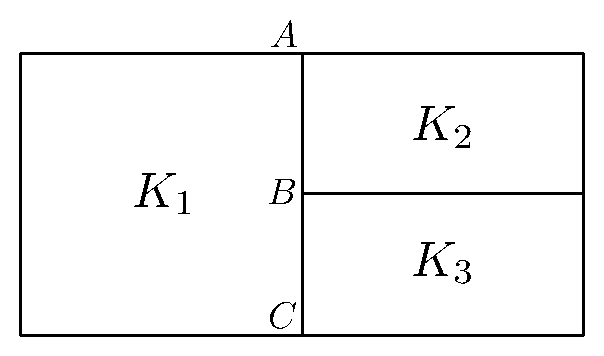
\includegraphics[scale=0.75]{./fig/hangingNode.eps}
\caption{Schematic of a hanging node: the element on the right has been refined, resulting in a ``broken'' edge along the right side of the coarse element $K_{1}$.
}
\label{fig:hangingNode}
\end{figure}

Because we focus on implementing DPG solvers, we can make certain simplifying assumptions.  We can assume a first-order system with all derivatives moved onto test functions.  We can assume that trial space variables defined on element interiors are discontinuous across element boundaries; the inter-element ``connectivity'' is limited to fluxes and traces, which are defined only on the element boundaries.  The latter allows some flexibility in dealing with hanging nodes.

Camellia aims at a higher level of abstraction than does \deal; for instance, Camellia does not require the user to write a loop over the elements in the mesh to compute the stiffness matrix.  In fact, the user need not be directly aware of the stiffness matrix at all.  There is a tradeoff here: while this has obvious advantages in that the code is generally simpler and easier to write, if the user wishes to do something special with the stiffness matrix, she might find that it is not as obvious how to do so in Camellia as it is in \deal.  In Camellia, specification of variational forms and test space inner products hews quite closely to the mathematics; for instance, the code snippet below specifies:
\begin{itemize}
\item a field trial variable $u \in L^{2}$,
\item a trace trial variable $\widehat{u} \in H^{1/2}$,
\item a test variable $\vect{v} \in \NVRHdiv$,
\item a bilinear form $b(u,v) = -\int_{\Omega} u \NVRdiv \vect{v} + \int_{\partial \Omega} \widehat{u} \vect{v} \cdot \vect{n} $, and
\item a test space norm $\norm{\vect{v}}_{V}^{2} = \norm{\vect{v}}_{L^{2}}^{2} + \norm{\NVRdiv \vect{v}}_{L^{2}}^{2}$.
 \end{itemize}

\begin{lstlisting}
  VarFactory varFactory; 
  // define field variable u
  VarPtr u = varFactory.fieldVar("u");
  // define flux variable u_hat
  VarPtr u_hat = varFactory.traceVar("\\widehat{u}");
  // define test function v
  VarPtr v = varFactory.testVar("v", HDIV); 
  // create bilinear form
  BFPtr bilinearForm = Teuchos::rcp( new BF(varFactory) );
  // specify field variable term
  bilinearForm->addTerm(-u, v->div());
  // specify flux variable term
  bilinearForm->addTerm(u_hat, v->dot_normal());
  // create test space inner product
  IPPtr innerProduct = Teuchos::rcp(new IP);
  // add L^2 term
  innerProduct->addTerm(v);
  // add divergence term
  innerProduct->addTerm(v->div());
\end{lstlisting}

Our approach in Camellia can perhaps be seen as falling somewhere between \deal and FEniCS---the specification of variational forms is at least vaguely reminiscent of FEniCS's UFL, but we are not going so far as to provide a domain-specific language and C++ code generation for that language.  We do include some basic operator overloading to allow expressions in variational forms such as \code{sinx * u1 + cosy * u2}, where \code{sinx} and \code{cosy} are user-supplied pointers to a \code{Function} class instance.

At present, Camellia supports only two spatial dimensions, and has no direct support for a time domain.  We do hope to add support for one, two, and three space dimensions, as well as extrusion of any of these in a time dimension to create space-time elements.  In 2D, Camellia supports both quads and triangles; our hope is to support at least hexahedra and tetrahedra (and perhaps pyramids and prisms) in 3D.  This is in contrast to \deal, which for the sake of simplicity of the code supports only hypercube elements, and FEniCS, which supports only simplicial elements.

One of the great advantages of DPG is that we can \emph{measure}, not merely estimate, the error in the dual norm $\norm{\cdot}_{V'}$, which is exactly the natural norm from a mathematical point of view (of course it is up to the analyst to specify $\norm{\cdot}_{V}$ well).  We can use this to drive adaptivity, and because this depends simply on the choice of norm $\norm{\cdot}_{V}$, the user need not implement an error indicator.  At present, we support both $h$- and $p$-adaptivity; $hp$-refinements are also possible, although we do not yet have a general strategy for deciding between $h$ and $p$.  Similarly, the infrastructure for refinements could easily be extended to support anisotropic refinements, but we do not yet have a strategy for deciding the best refinement direction.  Some examples using adaptivity are discussed in Section \ref{sec:preliminaryResults} and Appendix \ref{sec:StokesNumericalResults}.

Camellia supports distributed computation of the stiffness matrix; because the computation of optimal test functions is a local problem, this scales perfectly.  We do not yet support distributed storage of the mesh or solution---a copy of each is stored on each processor---although we do hope to add both.  Currently, we use KLU and MUMPS solvers, which are both direct solvers; MUMPS is a parallel solver.  Camellia implements an abstract \code{Solver} interface, by which users can add linear solvers of their own choosing.  (Determining good preconditioners for DPG stiffness matrices is an area of active research.)  Detailed discussion of the distribution of the stiffness matrix and some measurements of the scalability of various parts of the code can be found in Appendix \ref{sec:CamelliaDetails}.

\paragraph{The Factory Design Pattern.}
Camellia represents each basis function that corresponds to a trial or test space variable on a given cell using an instance of Intrepid's \code{Basis} class.  If each cell in the mesh were to store a \code{Basis} object for each basis, that would be a waste both of memory and the time required to construct the objects.  For this reason, we make use of the \emph{Factory} design pattern, which encapsulates object construction---in this instance, we want only to create each basis once on each compute node (to be precise, this is the FlyWeightFactory design pattern \cite[p. 199]{GoFBook}).  When the \code{BasisFactory} receives a request for a basis belonging to a given function space (e.g. \NVRHdiv) on a given cell topology (e.g. a triangle) with a given polynomial order (e.g. 5), it looks up this combination of features in a hash map; if such a basis already exists, a pointer to it is returned; if it does not exist, it is created and stored, and a pointer to it is returned.

Discrete spaces in Camellia are represented by the \code{DofOrdering} class,\footnote{We are considering renaming this class \code{DiscreteSpace}.} and the combination of trial space and test space for an element comprise the \code{ElementType}.  Just as with \code{Basis}, the Factory pattern is applied in \code{DofOrderingFactory} and \code{ElementTypeFactory}.

It is worth noting that the Factory classes will not generally be used directly by users.  Creation of \code{DofOrdering}s and \code{ElementType}s is generally handled by the \code{Mesh} class; \code{Basis} instances are usually requested by the \code{DofOrderingFactory} and assigned to the \code{DofOrdering}.

\paragraph{Basis Values: \deal's \code{FEValues} compared with Camellia's \code{BasisCache}.}
Finite element computations often make use of a \emph{reference} cell; values of shape functions and derivatives are computed on the reference cell and  transformed to appropriate values in physical space.  The values of interest are usually at specific points; most commonly these are quadrature points.  Both \deal and Camellia include classes---\code{FEValues} and \code{BasisCache},\footnote{Because \code{BasisCache} has evolved somewhat to include additional features relating to the computational context---e.g., it can optionally store a list of the cell IDs currently being operated on---we are considering renaming it \code{ContextCache}.} respectively---that take advantage of this fact to reduce development effort and speed execution.

Both classes compute values in reference space and provide transformations into physical space.  Now, not all the basis function values will be of interest for a given computation---derivative values might not be required, for example, and it would be wasteful to compute them in such a case.  \deal allows the user to specify that such values are not required so that they will not be computed.  Camellia's approach is \emph{lazy} computation of all values: the first time, for example, the derivative values for a basis are requested, these will be computed at all the points of interest, and stored.

It is also worth noting that, while \deal's \code{FEValues} class is tied to a particular element type, \code{BasisCache} is a bit more flexible.  \code{BasisCache} will return values for any requested basis; it is possible to do so efficiently because all bases are created using the \code{BasisFactory}, as described above.  \code{BasisCache} uses the memory address of the \code{Basis} object as an index into its lookup tables.  Generally speaking, a \code{BasisCache} instance will be relatively short-lived in Camellia, but many methods do take a \code{BasisCache} pointer as an argument, so that basis values computed in one part of the code might easily be reused in a completely separate part of the code.

\begin{figure}[h!b!p!]
\centering
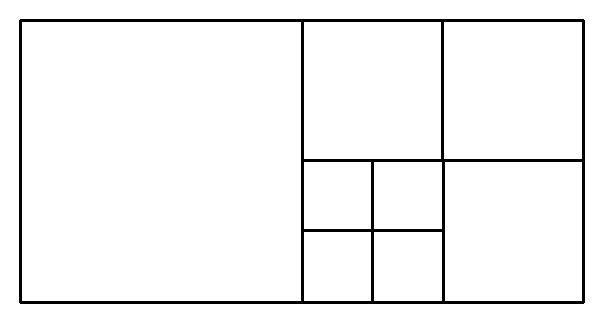
\includegraphics[scale=0.75]{./fig/hangingNode2irreg.eps}
\caption{Schematic of a 2-irregular mesh.
}
\label{fig:hangingNode2irreg}
\end{figure}

\paragraph{Treatment of Hanging Nodes: \code{MultiBasis}.}
As mentioned in the discussion of \deal in Section \ref{sec:litreviewFEM}, one of the usual complexities of finite element methods has to do with the treatment of \emph{hanging nodes}, element faces in the mesh where an element has been refined and its neighbor along that face has not, as shown in Figure \ref{fig:hangingNode}.  At issue is the relationship of the shape functions discretizing a variable on the coarse element to those discretizing the same variable on the finer neighboring elements.  (When neighboring elements are of the same coarseness and polynomial order, the relationship between shape functions on the neighbors is a simple identification.)

The usual way that hanging nodes are handled in finite elements is by imposing a constraint on the finer elements, so that their shape functions conform to the function space on the coarse element along the shared face.  Such constraints might become complicated to implement if arbitrary refinement patterns are allowed---for this reason, finite element codes sometimes limit the irregularity of the mesh;\footnote{\deal and libMesh both support meshes of arbitrary irregularity, although this is not the default option, and their mechanisms for implementing this necessarily differ from ours.} e.g., the mesh shown in Figure \ref{fig:hangingNode2irreg} is called \emph{2-irregular}, because the coarse neighbor on the right has been refined twice along the shared edge, while the one on the left has not been refined at all.  The usual practice is to enforce 1-irregularity by introducing additional refinements to coarse neighbors; usually this is implemented by means of constraints imposed on the appropriate degrees of freedom to ensure continuity.

Our approach in Camellia differs.  We observe that in DPG the discretizations on element interiors are entirely independent of each other, so that only the flux and trace variables---the ones that are defined along a shared edge---need to be reconciled.  We therefore allow the coarse element ($K_{1}$ in Figure \ref{fig:hangingNode}) to ``borrow'' the appropriate basis from its finer neighbors.  The result is that the coarse element has a basis that is only piecewise polynomial along the shared edge; in the case of fluxes, the basis even allows discontinuity at the hanging node.

To implement this, we define a general basis class, which we call \code{MultiBasis}, which allows a basis to be formed along a broken edge from two arbitrary sub-bases.  Clearly, to avoid introducing quadrature error, the quadrature points for the \code{MultiBasis} must be the union of those for its sub-bases; therefore, \code{MultiBasis} provides these to the \code{BasisCache} when the latter determines quadrature points for an edge.  Because a sub-basis can itself be a \code{MultiBasis}, we have an elegant recursive mechanism by which we can handle meshes of arbitrary irregularity.\footnote{Thus far in practice, we have usually continued to enforce 1-irregularity, but in the instances where we have not enforced it, we have not found any ill effects.}

Dual to the concept of \code{MultiBasis} is that of a \code{PatchBasis}, in which the finer elements ``borrow'' a patch of the coarse neighbor's basis.  An option for \code{PatchBasis} is under development.  The \code{PatchBasis} approach coincides exactly with the standard approach of imposing constraints on the finer elements.

\section{Summary of Preliminary Results}
\label{sec:preliminaryResults}
In this section, we summarize the results we have thus far achieved in the context of the Stokes problem.  The principal theoretical result is the proof of the well-posedness of the velocity-gradient-pressure Stokes formulation (specified below), which implies optimal convergence rates when the \emph{graph norm} is used as the norm on the test space.  Details are provided in Appendix \ref{sec:StokesAnalysis}.

As can be seen by the large body of research discussed in Section \ref{sec:litreviewflow}, finding good discrete spaces for the
Stokes problem is \emph{difficult}---this has been an area of ongoing
research for decades.  Through our analysis and numerical results, we demonstrate that DPG allows
solution of the Stokes problem without any special effort---that is,
the Stokes problem is approached and analyzed with exactly the same
DPG-theoretical tools that we use for other linear problems, and we
can use the same discrete spaces for velocity and pressure. In
particular, we use equal-order spaces for velocity and pressure, and
both pressure and velocity converge at the same rate, a contrast with
LDG \cite{CockburnKanschatSchotzauSchwab03}.  Indeed, one of our
numerical experiments demonstrates not only that the method delivers
the optimal convergence rate, but also that the method provides a solution
close to the $L^{2}$ projection of the exact solution.

Our Stokes work began in collaboration with Pavel Bochev and Denis
Ridzal in the summer of 2010 \cite{RobertsetAl10}, during an
internship at Sandia.  Bochev astutely suggested the Stokes problem as
a good example problem for DPG.  That summer, we were puzzled by the
poor performance of DPG using what we herein refer to as the
\emph{naive} test space norm; the present analysis serves (among other
things) to explain why the naive norm fails to achieve optimal
convergence rates, in contrast to the choice to which our analysis
leads us, which we here call the \emph{adjoint graph} norm.

Our numerical results fall into two categories: convergence studies performed on a manufactured solution to verify the theoretically predicted convergence rates, and adaptivity studies in the context of the lid-driven cavity flow problem.  Further details, including an exploration of how the method can go wrong if the test space norm is naively chosen, can be found in Appendix \ref{sec:StokesNumericalResults}.

\subsection{Velocity-Gradient-Pressure Formulation.} The classical strong form of the Stokes problem in $\Omega \subset
\mathbb{R}^{2}$ is given by
\begin{subequations}
\begin{align}
- \mu \Delta \vect{u} + \NVRgrad p &= \vect{f} & \text{ in } \Omega, \label{NVR:eq:StokesFirstIntro} \\
\NVRdiv \vect{u} &= g & \text{ in } \Omega, \\
\vect{u} &= \vect{u}_D & \text{ on } \partial\Omega,\label{NVR:eq:StokesLastIntro}
\end{align}
\end{subequations}
where $\mu$ is viscosity, $p$ pressure, $\vect{u}$ velocity, and
$\vect{f}$ a vector forcing function.  The first equation corresponds
to conservation of momentum, and the second to conservation of mass.
While the analysis will treat the case where mass can be added or removed
from the system ($g \neq 0$), in practice generally (and in our
numerical experiments) $g = 0$.  Since by appropriate
non-dimensionalization we can eliminate the constant $\mu$, we take
$\mu=1$ throughout.

In order to apply the DPG method, we need to cast the system
\eqref{NVR:eq:StokesFirstIntro}--\eqref{NVR:eq:StokesLastIntro} as a
first-order system.  We introduce $\NVRtensor{\sigma}= \NVRgrad
\vect{u}$:
\begin{subequations}
\begin{align}
- \NVRdiv \NVRtensor{\sigma} + \NVRgrad p &= \vect{f} & \text{ in } \Omega, \\
 \NVRdiv \vect{u} &= g & \text{ in } \Omega, \\
 \NVRtensor{\sigma} - \NVRgrad \vect{u} &= 0 & \text{ in } \Omega,\\ 
\vect{u} &= \vect{u}_D & \text{ on } \partial\Omega.
\end{align}
\end{subequations}

Clearly, the first-order formulation is by no means unique; we have chosen this one for convenience of mathematical analysis
and simplicity of presentation.  Previously, we have experimented with
other formulations; the velocity-stress-pressure (VSP) and the velocity-vorticity-pressure (VVP) formulations \cite{RobertsetAl10,RobertsetAl11}.\footnote{The VSP and VVP Stokes formulations are also detailed and used in Appendix \ref{sec:CamelliaDetails} as part of the verification of Camellia.}  Note also that $\NVRtensor{\sigma}$ in this formulation is \emph{not} the physical stress (the physical stress does enter the VSP formulation).

\subsection{Manufactured Solution.}
To test the method, we use a manufactured solution following Cockburn et al. \cite{CockburnKanschatSchotzauSchwab03}
\begin{align*}
u_{1} &=  -e^{x} ( y \cos y + \sin y )\\
u_{2} &=  e^{x}  y \sin y\\
p &= 2 \mu e^{x} \sin y
\end{align*}
on domain $\Omega = (-1,1)^2$, taking $\mu=1$, with uniform quadrilateral meshes of increasing granularity, and examine convergence rates.  The $L^{2}$ norm of the exact solution for $u_{1}$ is 2.53; for $u_{2}$, 1.07; for $p$, 2.81.

Figure \ref{fig:summary_graph_h} shows $h$-convergence results using the graph norm in the test space, for uniform quadrilateral meshes varying from $k=1$ to 4 in polynomial order, and from $1 \times 1$ to $16 \times 16$ elements.  The dashed lines in the plots show the error of an $L^{2}$ projection of the exact solution (the theoretical best we could achieve)---the lines lie nearly on top of each other.  We not only observe optimal convergence rates, but almost exactly achieve the best approximation error!

\begin{figure}[p]
\centering
\subfigure[$u_{1}$]{
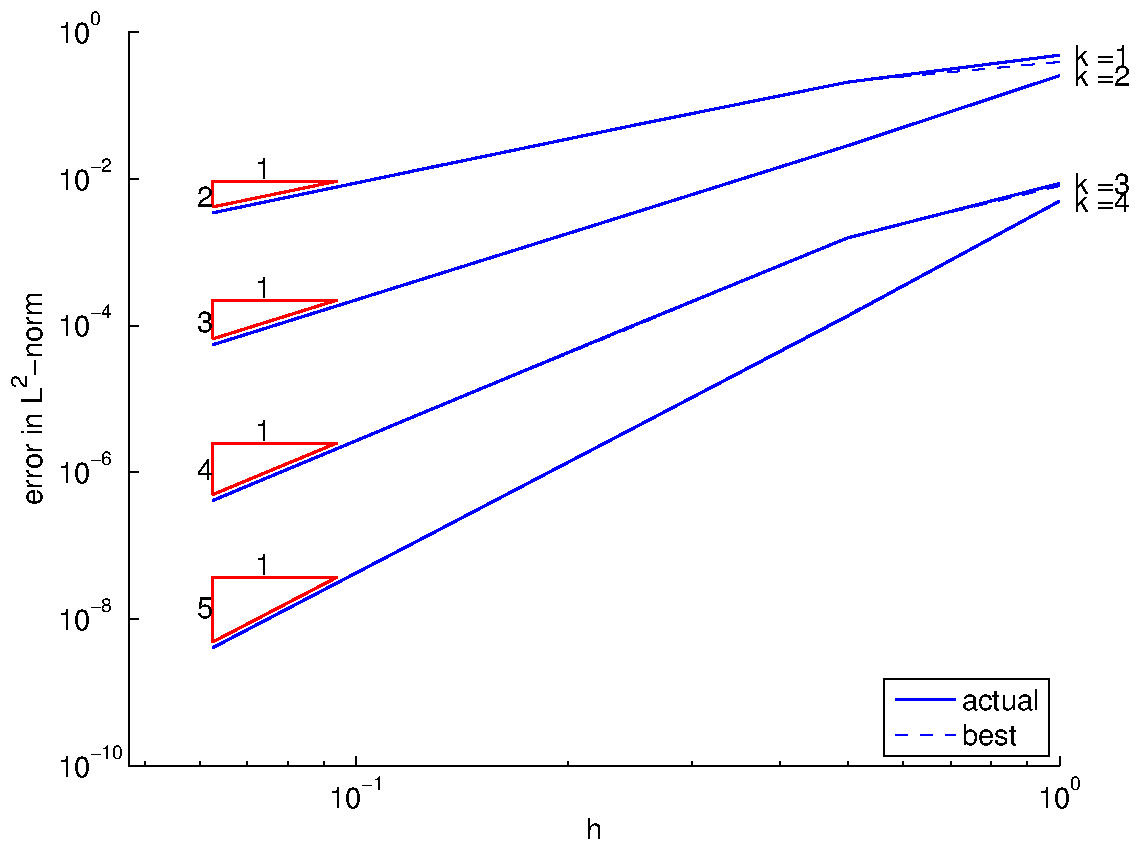
\includegraphics[scale=0.42]{./figures/u1_graph_h.pdf}
\label{fig:u1graph_h}
}
\subfigure[$u_{2}$]{
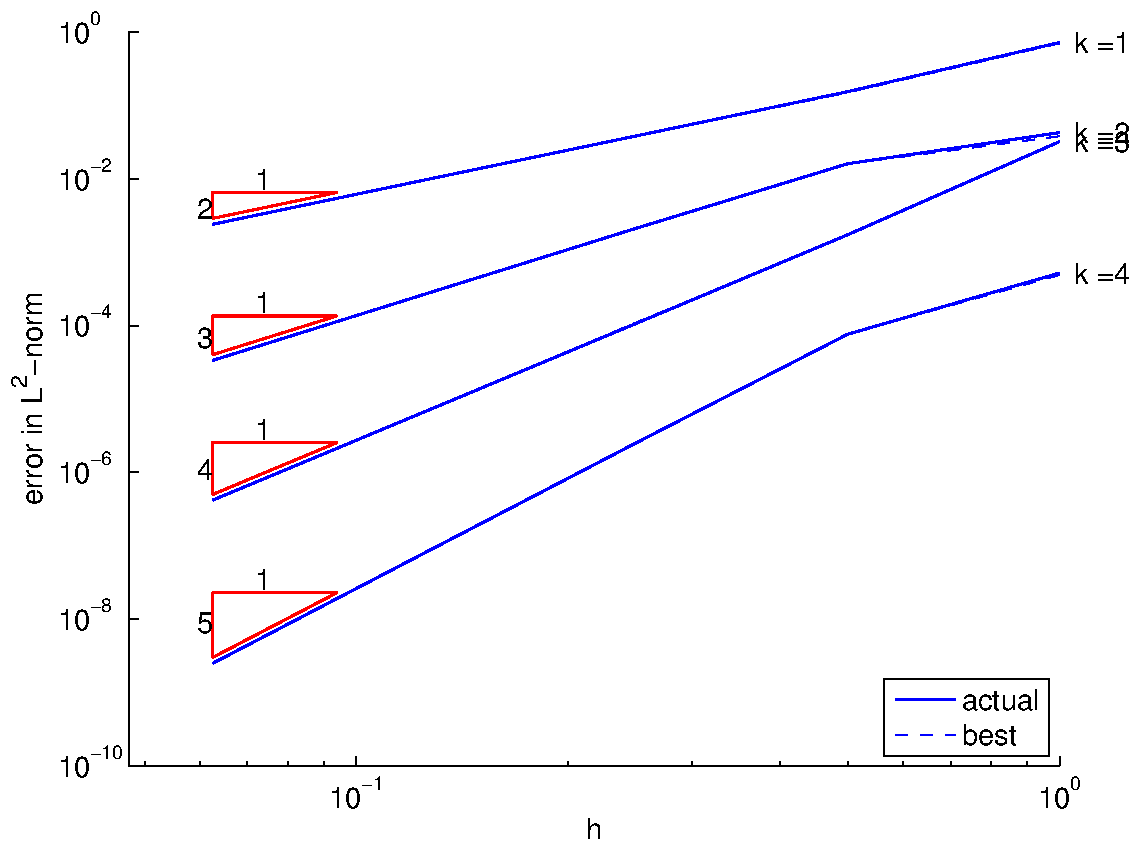
\includegraphics[scale=0.42]{./figures/u2_graph_h.pdf}
\label{fig:u2graph_h}
}
\subfigure[$p$]{
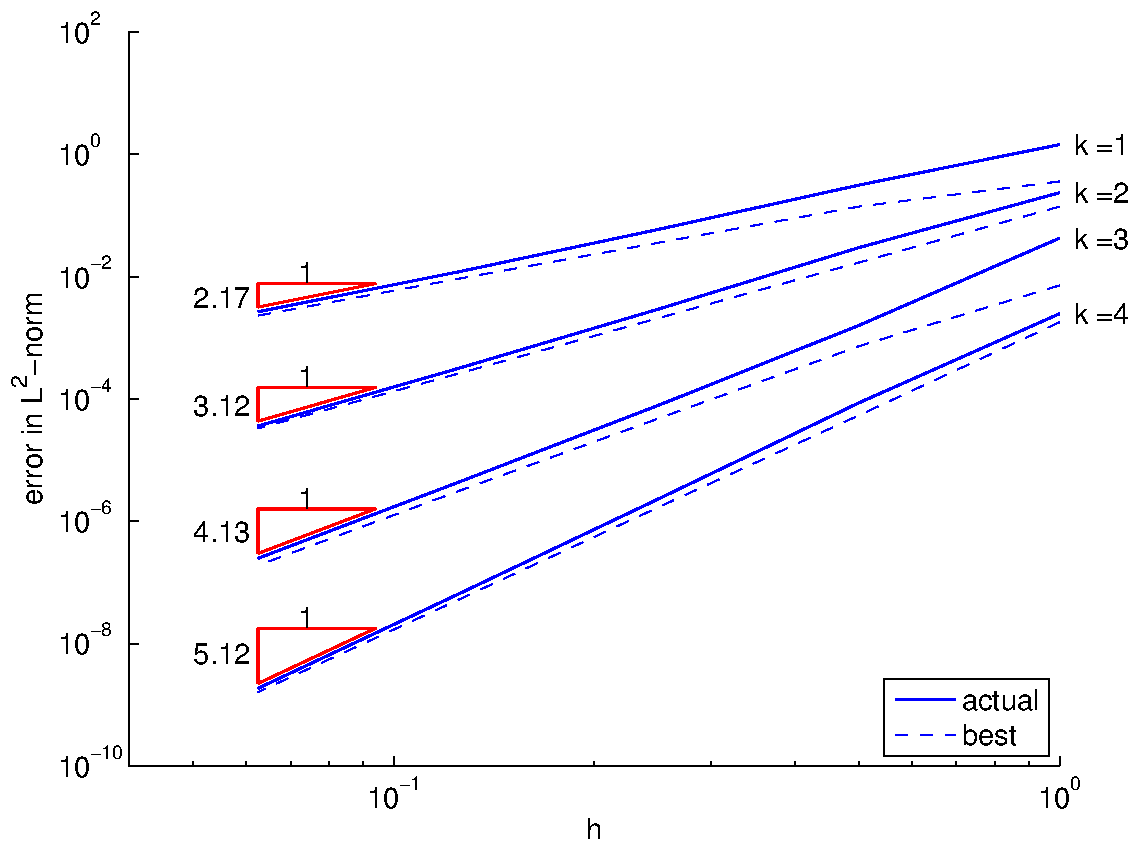
\includegraphics[scale=0.42]{./figures/pressure_graph_h.pdf}
\label{fig:pressuregraph_h}
}
\caption{$h$-convergence of $u_{1},u_{2}$ and $p$ when using the graph norm for the test space.  We observe optimal convergence rates, and nearly match the $L^{2}$-projection of the exact solution.
}
\label{fig:summary_graph_h}
\end{figure}

\subsection{Lid-Driven Cavity Flow.}\label{sec:lidDrivenCavityFlow}
\begin{figure}[h!b!p!]
\centering
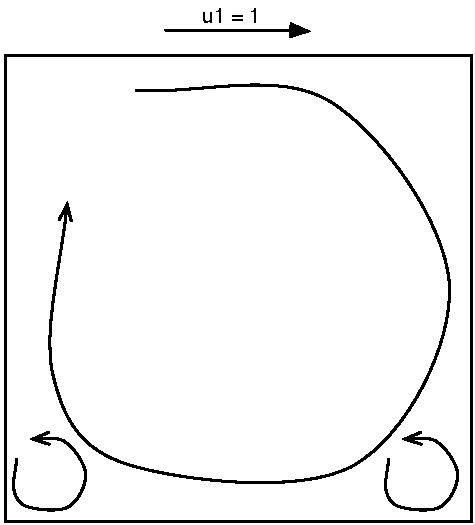
\includegraphics[scale=0.75]{./figures/cavity_flow_cartoon.pdf}
\caption{Sketch of lid-driven cavity flow.
}
\label{fig:summary_cavity_flow_cartoon}
\end{figure}
A classic test case for Stokes flow is the lid-driven cavity flow problem.  Consider a square cavity with an incompressible, viscous fluid, with a lid that moves at a constant rate.  The resulting flow will be vorticular; as sketched in Figure \ref{fig:summary_cavity_flow_cartoon}, there will also be so-called \emph{Moffat eddies} at the corners; in fact, the exact solution  will have an infinite number of such eddies, visible at progressively finer scales \cite{Moffat}.  Note that the problem as described will have a discontinuity in the fluid velocity at the top corners, and hence its solution will not conform to the spaces we used in our analysis; for this reason, in our experiment we approximate the problem by introducing a thin ramp in the boundary conditions---we have chosen a ramp of width $\frac{1}{64}$.  This makes the boundary conditions continuous,\footnote{It is worth noting that these boundary conditions are not exactly representable by many of the coarser meshes used in our experiments.  We interpolate the boundary conditions in the discrete space.} so that the solution conforms to the spaces used in the analysis.
\paragraph{$h$-adaptivity study.}
For $h$-refinements, our strategy---previously discussed in Section \ref{sec:proposedApproachDPG}---is very simple:
\begin{enumerate}
\item Loop through the elements, determining the maximum element error $\norm{e_{K{\rm max}}}_{V}$.
\item Refine all elements with error at least 20\% of the maximum $\norm{e_{K{\rm max}}}_{V}$.
\end{enumerate}

Because the exact solution is unknown, we first solve on an overkill mesh and compare our adaptive solution at each step to the overkill solution.  In this experiment, we used quadratic field variables ($k=2$), a test space enrichment of 1 relative to the $H^{1}$ order (that is, $k_{\rm test} = k + 2 = 4$) for both the adaptive and overkill solutions.  The overkill mesh was $256 \times 256$ elements, with 5,576,706 dofs.

The initial mesh was a $2 \times 2$ square mesh; we ran seven $h$-adaptive refinements.  We stopped after seven steps to ensure that the resulting mesh was nowhere finer than the overkill solution.  At each step, we computed the Euclidean ($\ell_{2}$) norm of the $L^{2}$ norm of each of the seven field variables.  The final adaptive mesh has 124 elements and 11,202 dofs, and combined $L^{2}$ error of $4.4 \times 10^{-4}$ compared with the overkill mesh.  We also ran a few uniform refinements and computed the $L^{2}$ error for these compared with the overkill mesh, to show the comparative efficiency of the adaptive refinements.  The results are plotted in Figure \ref{fig:summary_adaptive_cavity_flow_quadratic_vs_overkill}.
\begin{figure}[h!b!p!]
\centering
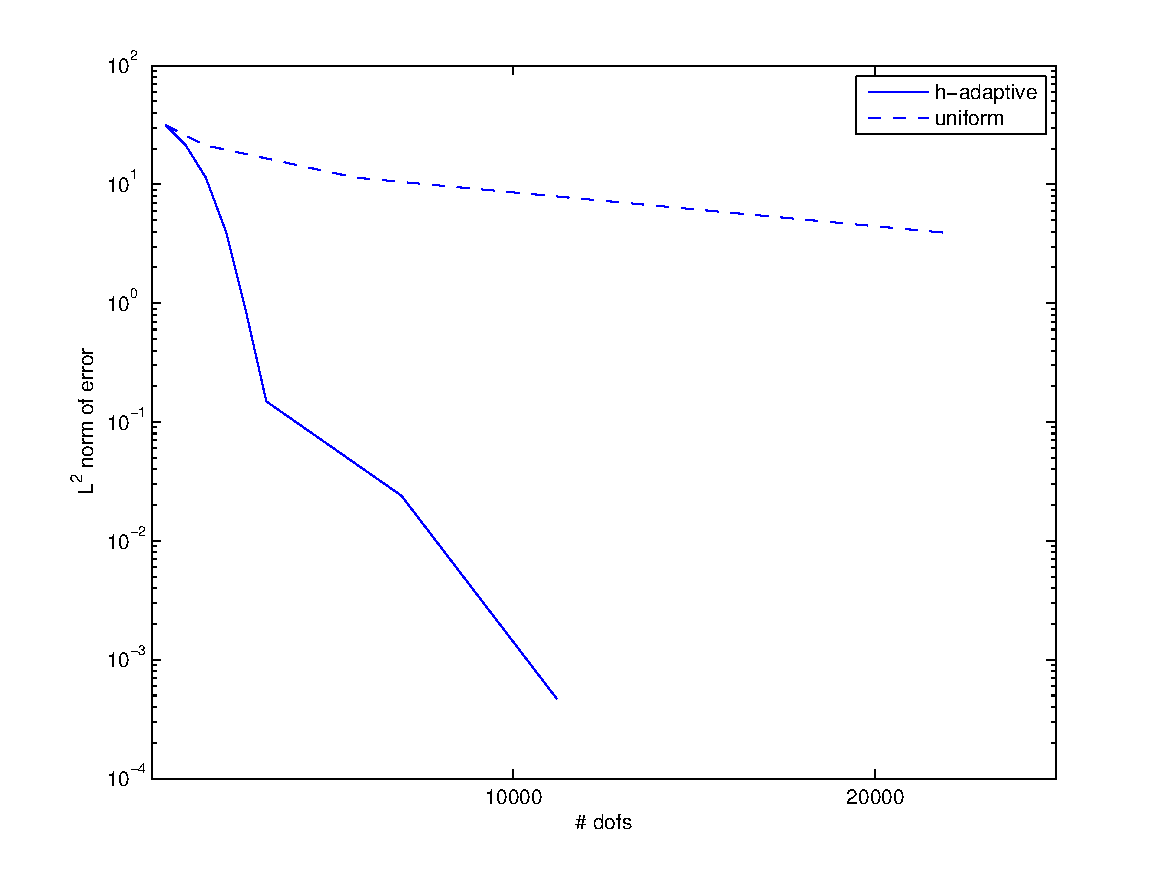
\includegraphics[scale=0.60]{./figures/adaptive_cavity_flow_quadratic_vs_overkill.pdf}
\caption{Euclidean norm of $L^{2}$ error in all field variables in $h$-adaptive mesh relative to an overkill mesh with $256 \times 256$ quadratic elements.  The Euclidean norm of all field variables in the exact solution is 6.73.
}
\label{fig:summary_adaptive_cavity_flow_quadratic_vs_overkill}
\end{figure}

We also post-processed the results to solve for the stream function $\phi$, where $\Delta \phi = \NVRcurl \vect{u}$.  The contours of $\phi$ are the streamlines of the flow.  These are plotted for the quadratic adaptive mesh described above in Figure \ref{fig:summary_streamlines_p2}; the first Moffat eddy can be seen clearly in the zoomed-in plot.  This quadratic mesh does not resolve the second Moffat eddy, but if we run 11 adaptive refinements on a cubic mesh, we can see it.  This is shown in Figure \ref{fig:summary_streamlines_p3_r11}.

\begin{figure}[p]
\centering
\subfigure[full cavity]{
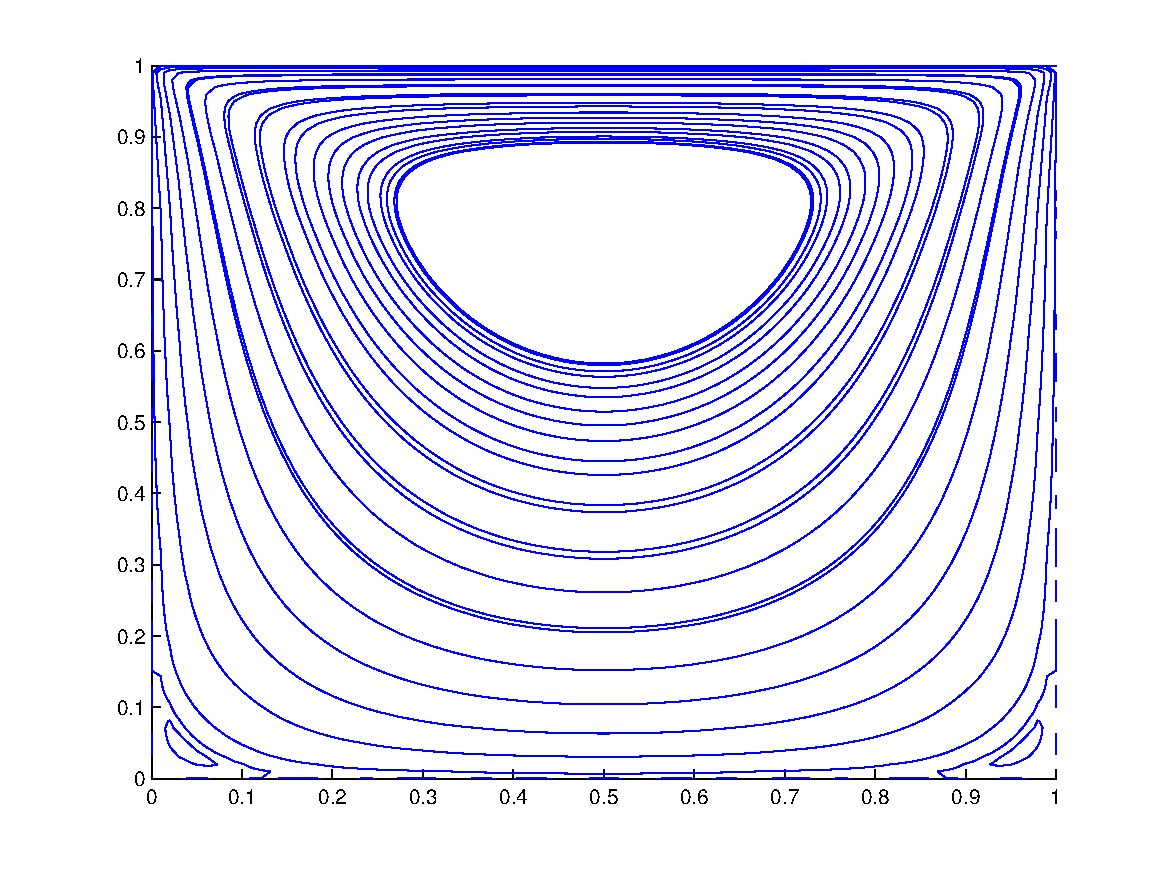
\includegraphics[scale=0.42]{./figures/streamlines_p2_r7.pdf}
\label{fig:summary_streamlines_p2_r7}
}
\subfigure[lower-left corner]{
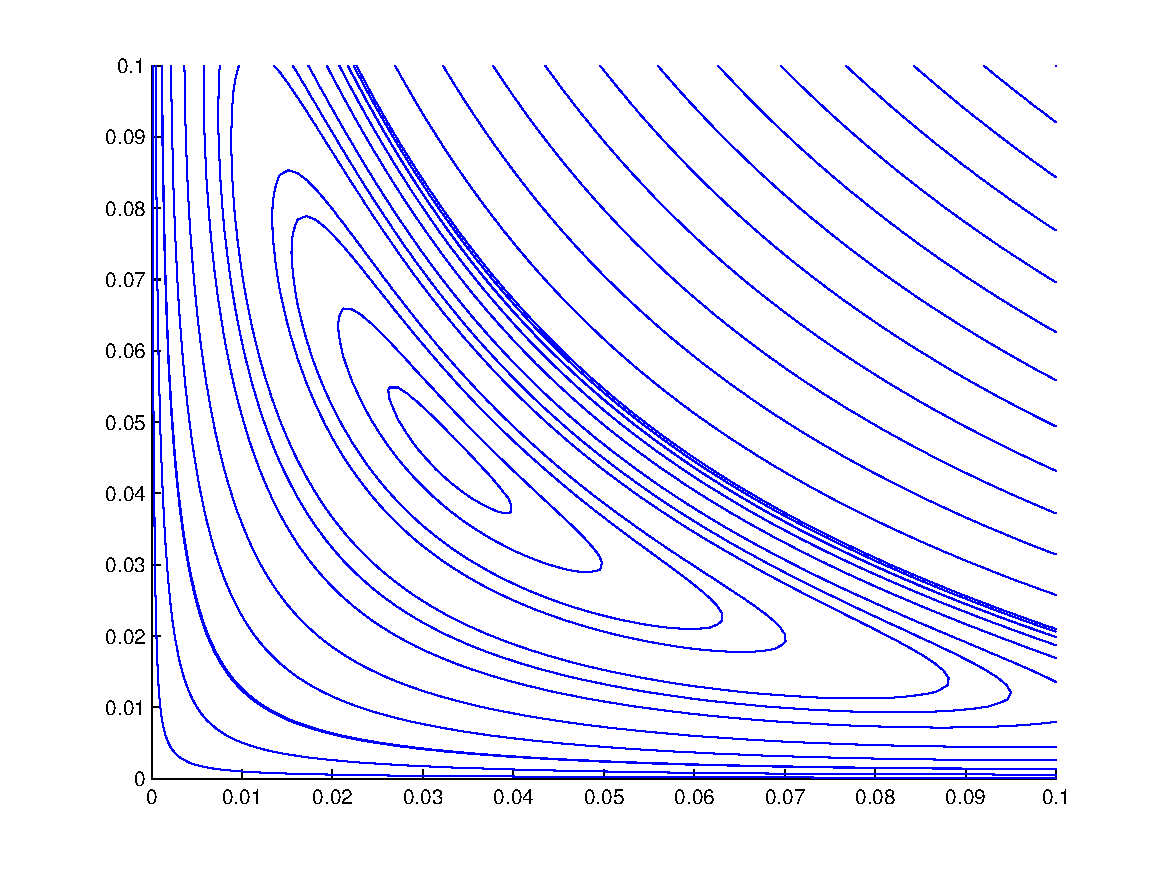
\includegraphics[scale=0.42]{./figures/streamlines_detail_p2_r7.pdf}
\label{fig:summary_streamlines_detail_p2_r7}
}
\caption{Streamlines for the full cavity and for the lower-left corner, on a quadratic mesh after 7 adaptive refinements.  The lower-left corner shows the first Moffat eddy.  The final mesh has 124 elements and 11,202 dofs.}
\label{fig:summary_streamlines_p2}
\end{figure}

\begin{figure}[p]
\centering
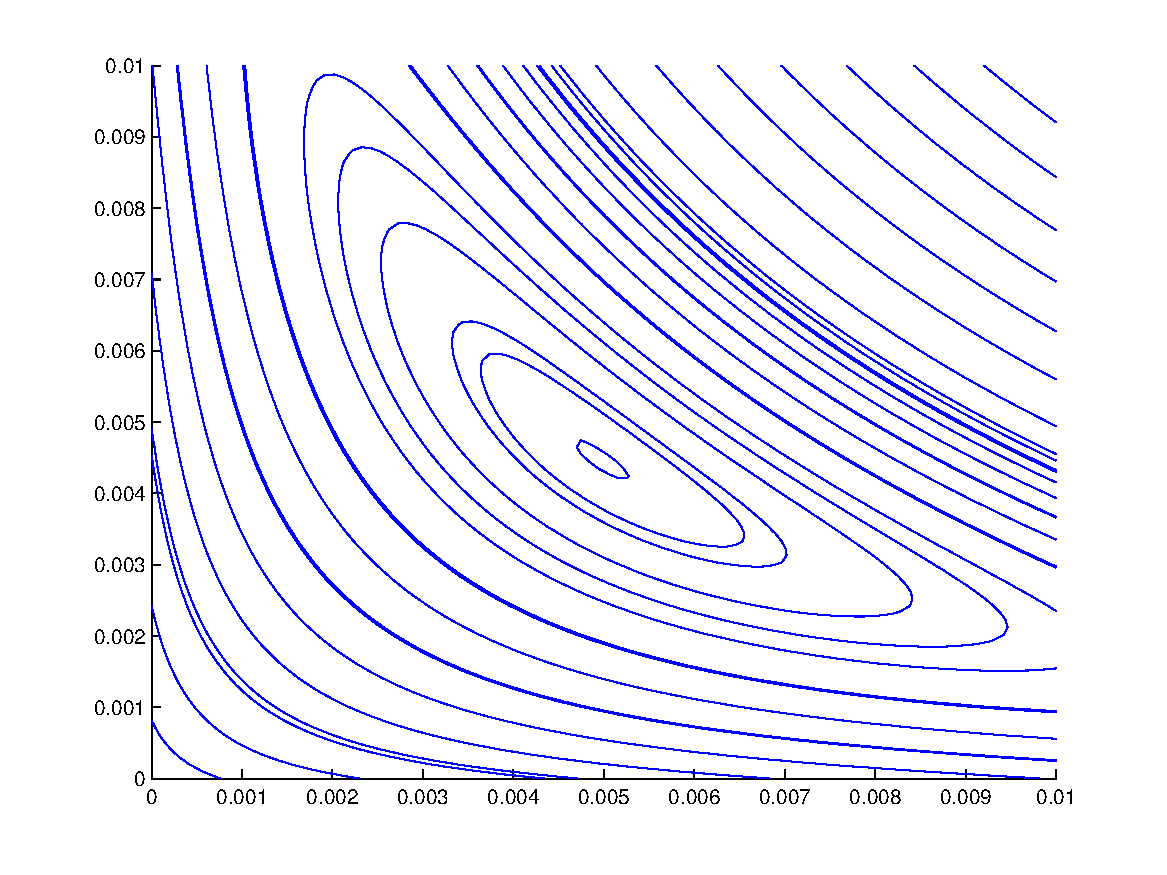
\includegraphics[scale=0.42]{./figures/streamlines_minute_detail_p3_r11.pdf}
\caption{Streamlines for the lower-left corner on a cubic mesh after 11 adaptive refinements: the second Moffat eddy.  The final mesh has 298 elements and 44,206 dofs.}
\label{fig:summary_streamlines_p3_r11}
\end{figure}

\paragraph{ad hoc $hp$-adaptivity study.}
\begin{figure}[h!b!p!]
\centering
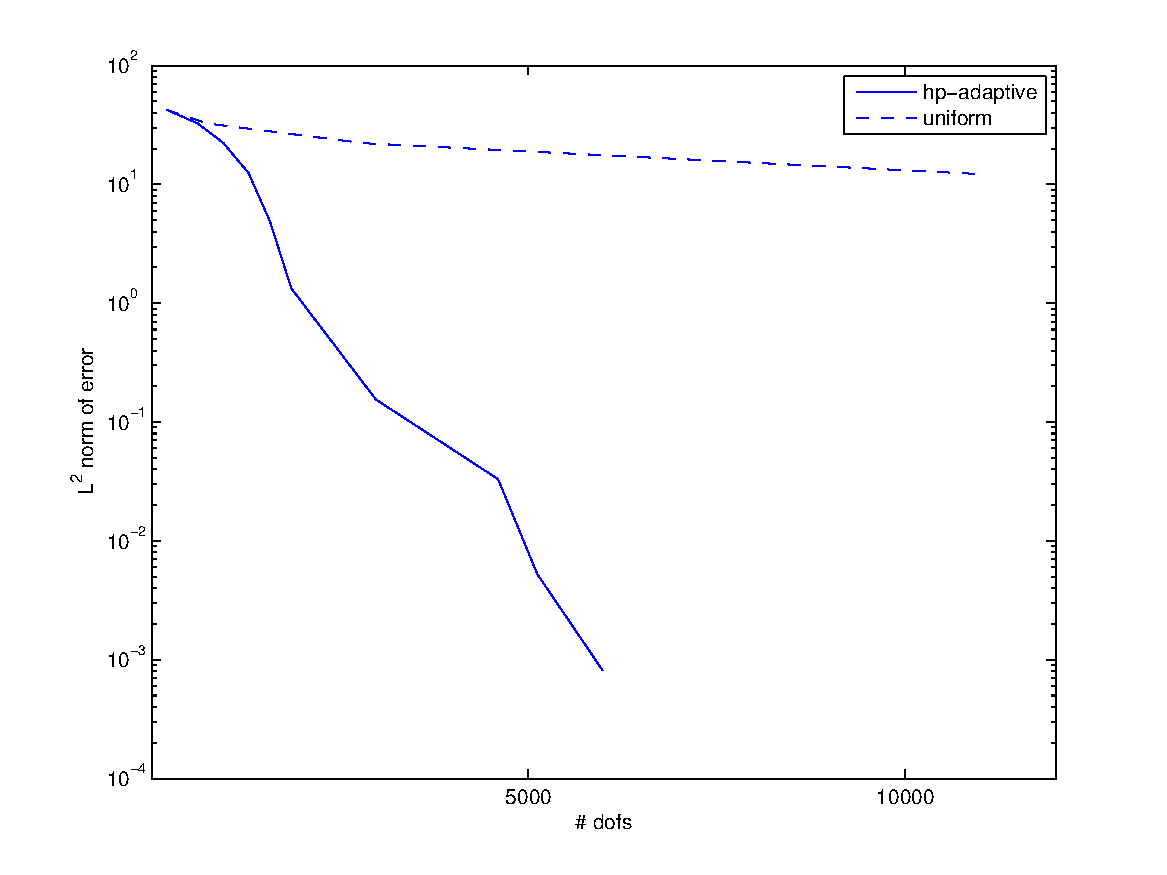
\includegraphics[scale=0.60]{./figures/hp_adaptive_cavity_flow_vs_overkill.pdf}
\caption{Euclidean norm of $L^{2}$ error in all field variables in (ad hoc) $hp$-adaptive mesh relative to an overkill mesh with $64 \times 64$ quintic elements.  The Euclidean norm of all field variables in the exact solution is 6.73; the final mesh has 46 elements and 5,986 dofs.
}
\label{fig:summary_hp_adaptive_cavity_flow_vs_overkill}
\end{figure}
For the $hp$ experiment, we adopt a similar strategy; this time, our overkill mesh contains $64 \times 64$ quintic elements, and our initial mesh has $2 \times 2$ linear elements.  We detail our ad hoc choice between $h$- and $p$-refinement in Appendix \ref{sec:StokesNumericalResults}; here, we simply note that our strategy for making this choice does depend on knowledge of the problem---we aim here simply to demonstrate that the method allows arbitrary meshes of arbitrary, variable polynomial order.

We ran 9 refinement steps.  The final mesh has 46 elements and 5,986 dofs, compared with 1,223,682 dofs in the overkill mesh.  The $L^{2}$ error of the adaptive solution compared with the overkill is $8.0 \times 10^{-4}$.  As in the previous experiment, we also tried running a few uniform $h$-refinements on the same initial mesh, as a baseline for comparison.  The results are plotted in Figure \ref{fig:summary_hp_adaptive_cavity_flow_vs_overkill}.

%pagebreaks provide a ``honeypot'' to keep too many figures from spilling into the conclusion
%\pagebreak

\section{Conclusion and Proposed Contributions}
\label{sec:conclusion}
The central contribution of the dissertation will be the design and development of mathematical techniques and software, based on the DPG method, for solving the 2D incompressible Navier-Stokes equations in the laminar regime (Reynolds numbers up to about 1000).  Along the way, we will investigate approximations to these equations---the Stokes equations and the Oseen equations---followed by the steady-state Navier-Stokes equations.  If time allows, we will also solve the transient Navier-Stokes equations.

The study of DPG applied to a system of PDEs has several aspects.  A first-order variational formulation must be derived, including the selection of appropriate test and trial space norms.  The well-posedness of the formulation might be proved.  The formulation can be investigated numerically by means of test problems: convergence can be studied by means of manufactured solutions, and ``real-world'' performance can be studied by means of more physically realistic test problems.  In terms of the CSEM program areas, the derivation of variational formulations and any proofs of their well-posedness belong to Area A, Applicable Mathematics.  The design and development of software for numerical investigations belong to Area B, Numerical Analysis and Scientific Computation.  The study of test problems belongs to Area C, Mathematical Modeling and Applications.  We will briefly describe the specific proposed contributions of this dissertation to each of these in turn.

\paragraph{Area A.}  We will pose several DPG formulations of the Stokes equations---the velocity-gradient-pressure (VGP), velocity-stress-pressure (VSP), and velocity-vorticity-pressure (VVP) formulations.  We will pose DPG formulations of the Oseen equations and the 2D incompressible Navier-Stokes equations.

We will prove the well-posedness of the VGP Stokes formulation for DPG, which has as consequence a guarantee of optimal convergence rates \cite{DPGStokes}; we plan to complete similar proofs for the VSP and VVP formulations.  Time permitting, we would like to prove a similar result for the Oseen equations.  The work on the Oseen equations will include the study of \emph{robustness} for the small-viscosity (high Reynolds number) case, with reference to previous work on convection-dominated diffusion \cite{DPG2,DemkowiczHeuer}.

\paragraph{Area B.} We will design and develop a software toolbox (\emph{Camellia}) for the investigation of DPG problems.  This will support 2D meshes of triangles and quads of variable polynomial order, provide mechanisms for easy specification of DPG variational forms, support $h$- and $p$- refinements, and support distributed computation of the stiffness matrix, among other features.

Time permitting, we hope to add support for meshes of arbitrary spatial dimension, support for space-time elements, and support for distributed mesh and solution representation.

\paragraph{Area C.} We will verify convergence rates for the Stokes, Oseen, and Navier-Stokes equations using manufactured solutions.

We will simulate the classical lid-driven cavity flow and backward-facing step problems using, in turn, the Stokes, Oseen, and Navier-Stokes equations.

We will simulate flow past a cylinder using the steady-state Navier-Stokes equations.  Time permitting, we will do so with the transient equations as well.

\pagebreak
\appendix
\section{Analysis of the Velocity-Gradient-Pressure Stokes Formulation}
\label{sec:StokesAnalysis}

The purpose of this appendix is to present a general theory for the DPG
method for linear PDEs and immediately specialize it to the Stokes
problem. The presented theory summarizes results obtained in
\cite{DPG6,BramwellDemkowiczGopalakrishnanQiu11,DemkowiczGopalakrishnanMugaZitelli12}
for particular boundary-value problems and specializes the
general theory for Friedrichs systems, presented in
\cite{Bui-ThanhDemkowiczGhattas11b}, for cases in which the traces of the graph spaces
are available.  As most of the technical results here are classical,
we have chosen a somewhat informal format of presentation.


\subsection{Notation and Definitions\label{section:notation}}


Let $\Omega$ denote a bounded Lipschitz domain in $\doubleIR^n, n=2,3$,\: with boundary
$\Gamma = \ptl \Omega$. We shall use the following standard energy spaces:
\[
\begin{array}{rl}
H^1(\Omega) & := \{ u \in L^2(\Omega) \: : \: \bfnab u \in \bfL^2(\Omega) \}, \\[8pt]
\bfH(\text{div},\Omega) & := \{ \bfsig \in \bfL^2(\Omega) \: : \: \text{div} \bfsig \in L^2(\Omega) \}, 
\end{array}
\]
with the corresponding trace spaces on $\Gamma$:
\[
\begin{array}{rl}
H^{1/2}(\Gamma) & := \{ 
{\hat{u} =} u\vert_{\Gamma}, \: u \in H^1(\Omega) \},
\\[8pt] H^{-1/2}(\Gamma) & := \{ {\hat{\sigma}_{n}} = (\bfsig \cdot
\bfn)\vert_{\Gamma} ,\: \bfsig \in \bfH(\text{div},\Omega) \},
\end{array}
\] 
where $\bfn$ denotes the outward normal unit vector to the boundary
$\Gamma$.  The definition of trace space $H^{1/2}(\Gamma)$ is
classical but far from trivial, see e.g.  \cite[pp. 96]{McLean}.  The
assumption on the regularity of the domain (being Lipschitz) is
essential; domains with ``cracks'' require a special and
non-classical treatment. When necessary, we will formalize the use of
the trace operator by identifying it with a separate symbol, 
\[
\text{tr} \: : \: H^1(\Omega) \ni u \to \text{tr } u = {\hat{u} =} u\vert_{\Gamma}
\in H^{1/2}(\Gamma).  
\] 
The space $H^{-1/2}(\Gamma)$ is the topological
dual of $H^{1/2}(\Gamma)$ and a second trace operator corresponding to it,
\[ \text{tr} \: : \: \bfH(\text{div},\Omega) \ni \bfsig \to \text{tr
} \bfsig = {\hat{\sigma}_n} = (\bfsig \cdot \bfn)\vert_{\Gamma} \in
H^{-1/2}(\Gamma),
\] 
is usually defined by the {\em generalized Green
  Formula}; see e.g. \cite[pp. 61]{Showalter} or
\cite[pp. 530]{FAbook}. Note that, unless otherwise stated, in this
paper we use the same trace notation ``tr'' for functions in both
$H^1(\Omega)$ and $\bfH(\text{div},\Omega)$.

We shall also use group variables consisting of multiple copies of functions from $H^1(\Omega),\bfH(\text{div},\Omega)$, and $H^{1/2}(\Gamma)$ or distributions from $H^{-1/2}(\Gamma)$. We will then switch to boldface notation:
\[
\begin{array}{rl}
\bfH^1(\Omega) & = H^1(\Omega) \times \ldots \times H^1(\Omega),\\[8pt]
\bfH^{1/2}(\Gamma) & = H^{1/2}(\Gamma) \times \ldots \times H^{1/2}(\Gamma), \\[8pt]
\bfH^{-1/2}(\Gamma) & = H^{-1/2}(\Gamma) \times \ldots \times H^{-1/2}(\Gamma),
\end{array}
\]
etc. In the case of tensors, the definitions will be applied row-wise:
$$
\bfsig = (\sigma_{ij}) \in \bfH(\text{\bf div},\Omega) \quad \Longleftrightarrow \quad
(\sigma_{i1},\ldots,\sigma_{in}) \in \bfH(\text{div},\Omega),\: i=1,\ldots,n.
$$

\paragraph*{Broken energy spaces.}

Let $\Omega$ be partitioned into finite elements $K$ such that
\[
  \overline{\Omega} = \bigcup_K  \bar{K},\: \quad K \text { open},
\]
with corresponding {\em skeleton} $\Gamma_h$ and {\em interior
  skeleton} $\Gamma_h^0$,
\[
\Gamma_h := \bigcup_K \ptl K\qquad \Gamma_h^0 := \Gamma_h - \Gamma.
\]
The usual regularity assumptions for the elements can essentially be relaxed. 
The elements may be general polygons in 2D, or polyhedra\footnote{Possibly curvilinear polyhedra.}
 in 3D (with triangular and quadrilateral
faces). Meshes may be {\em irregular}, i.e. with hanging nodes (see e.g. \cite[pp. 211]{hpbook}).
Also, at this point, we do not make any shape regularity assumptions.
By {\em broken} energy spaces we simply mean standard energy spaces defined element-wise:
\[
\begin{array}{rl}
H^1(\Omega_h) & := \prod_K H^1(K), \\[8pt]
\bfH(\text{div},\Omega_h) & := \prod_K \bfH(\text{div},K).
\end{array}
\]
With broken energy spaces, integration by parts is performed element-wise. 
For $\bfsig \in \bfH(\text{div},\Omega_h)$ and $v \in H^1(\Omega)$, we have
\[
\begin{array}{rl}
(\text{div}_h \bfsig, v)_{\Omega_h}  := &\ds \sum_K (\text{div} \bfsig, v)_K \\[8pt]
 = &\ds \sum_K \left( -(\bfsig, \bfnab v)_K 
+ {\langle\hat{\sigma}_n,\hat{v}\rangle _{\ptl K}} \right) \\[8pt]
 = &\ds - (\bfsig, \bfnab v) + {\underbrace{\sum_K 
\langle\hat{\sigma}_n,\hat{v}\rangle_{\ptl K}}
_{=: \langle\hat{\sigma}_n,\hat{v}\rangle_{\Gamma_h}}.}
\end{array}
\]
Here $(\cdot,\cdot)$ and $(\cdot,\cdot)_K$ denote the $L^2$-product over
the whole domain and element $K$, resp., and $\langle\cdot,\cdot\rangle_{\ptl K}$
stands for the duality pairing between $H^{-1/2}(\ptl K)$ and
$H^{1/2}(\ptl K)$.


Integration by parts leads naturally to the concept of the trace space over the skeleton $\Gamma_h$,
\[
H^{1/2}(\Gamma_h) := 
{
\left\{ \hat{v} = \{\hat{v}_K \} \in \prod_K H^{1/2}(\ptl K) \: :
\: \exists v \in H^1(\Omega) : v\vert_{\ptl K} = \hat{v}_K \right\}.}
\]
This is not a trivial definition. First of all, to be more precise, by
${v}\vert_{\ptl K}$ we mean the trace (for element $K)$
of the restriction of ${v}$ to $K$. Secondly,
$H^{1/2}(\Gamma_h)$ is a {\em closed} subspace of $\prod_K
H^{1/2}(\ptl K)$, as we shall show momentarily. For convenience, we
assume that all trace spaces are endowed with {\em minimum-energy
  extension norms}, i.e.,
\[
 \Vert {\hat{u}}\Vert_{H^{1/2}(\ptl K)} :=
\inf_{\substack{
E{\hat{u}} \in H^1(K)\\ 
E{\hat{u}}\vert_{\ptl K} = {\hat{u}}}}
\Vert E{\hat{u}} \Vert_{H^1(K)},
\]
etc. Let 
${\hat{u}}^n = \{ {\hat{u}}^n_K \} $ be a sequence of functions in
$H^{1/2}(\Gamma_h)$ converging in the product space to a limit ${\hat{u}} =
\{{\hat{u}}_K \} $. For each element $K$, ${\hat{u}}^n_K$ 
is the trace of restriction
${u}^n\vert_K$ for some ${u}^n \in H^1(\Omega)$.  By the definition of
norms, ${u}^n\vert_K \stackrel{n \to \infty}{\longrightarrow} 
{u}_K$ in $H^1(K)$, for
each element $K$. The delicate question is whether we can claim that
the union ${u}$ of ${u}_K$ is in $H^1(\Omega)$. But this follows from the
definition of distributional derivatives. Indeed, given a test function $\phi
\in \mathcal{D}(\Omega)$, we have for each $n$,
\[
 \int_\Omega {u}^n \frac{\ptl \phi}{\ptl x_i} = - \int_{\Omega}
\frac{\ptl {u}^n}{\ptl x_i} \phi 
\] 
or 
\[ \sum_K \int_K {u}^n \frac{\ptl
  \phi}{\ptl x_i} = - \sum_K \int_K \frac{\ptl {u}^n}{\ptl x_i} \phi.
\]
Passing to the limit with $n \to \infty$, we get 
\[ \int_\Omega {u}
\frac{\ptl \phi}{\ptl x_i} = - \sum_K \int_K \frac{\ptl {u}_K}{\ptl x_i}
\phi, 
\] 
which proves that the union of element-wise derivatives
$\frac{\ptl {u}_K}{\ptl x_i}$, a function in $L^2(\Omega)$, {\em is} the
distributional derivative of ${u}$. Consequently, ${u} \in H^1(\Omega)$.

Notice that we have not attempted to extend the classical definition
of the trace space $H^{1/2}(\Gamma)$ for Lipschitz boundary $\Gamma$
to a non-Lipschitz skeleton $\Gamma_h$.\footnote{The definition of a
  Lipschitz domain includes the assumption that the domain is on one
  side of its boundary, see \cite[pp. 89]{McLean}.}  This is not
impossible but much more technical (like for domains with cracks).

A similar construction holds for globally conforming $\bfsig \in \bfH(\text{div},\Omega)$
but broken $v \in H^1(\Omega_h)$:
\[
\begin{array}{ll}
(\bfsig, \bfnab_h v)_{\Omega_h} & := \ds \sum_K (\bfsig, \bfnab v)_K \\[8pt]
& \ds = \sum_K \left( - (\text{div} \bfsig, v)_K + \langle{\hat{\sigma}}_n,{\hat{v}}\rangle_{\ptl K} \right) \\[8pt]
& \ds = -(\text{div} \bfsig,v) + \underbrace{\sum_K \langle{\hat{\sigma}}_n,{\hat{v}}\rangle_{\ptl K}}_{=: \langle{\hat{\sigma}}_n, {\hat{v}}\rangle_{\Gamma_h}}.
\end{array}
\]
In this case, we are led to the definition of the trace space $H^{-1/2}(\Gamma_h)$:
\[
H^{-1/2}(\Gamma_h) := \left\{ {\hat{\sigma}}_n = \{ {\hat{\sigma}}_{Kn} \}\in \prod_K H^{-1/2}(\ptl K) \: : \: \exists \bfsig \in \bfH(\text{div},\Omega)
: {\hat{\sigma}}_{Kn} = (\bfsig \cdot \bfn)\vert_{\ptl K} \right\}.
\]
We equip both trace spaces over the mesh skeleton with minimum energy extension norms
\[
\begin{array}{rl}
\Vert {\hat{v}} \Vert_{H^{1/2}(\Gamma_h)} := \ds &\inf_{\substack{{u} \in H^1(\Omega)\\ {u}\vert_{\Gamma_h} = u}} 
\Vert {u} \Vert_{H^1(\Omega)} \quad \text{ and} \\[24pt]
\Vert {\hat{\sigma}}_n \Vert_{H^{-1/2}(\Gamma_h)} := \ds &\inf_{\substack{\text{\bfsig} \in \text{\bfH}(\text{div},\Omega)\\
(\text{\bfsig} \cdot \text{\bfn})\vert_{\Gamma_h} = {\hat{\sigma}}_n}}
\Vert \bfsig \Vert_{\text{$\bfH$}(\text{div},\Omega)}.
\end{array}
\]
We will also need the space of traces on the internal skeleton
\[
\tilde{H}^{1/2}(\Gamma_h) := \left\{ {\hat{v}} = \{{\hat{v}}_K \} \in  \prod_K H^{1/2}(\ptl K) \: : \: \exists {v} \in H^1_0(\Omega) : {v}\vert_{\ptl K} = {\hat{v}}_K \right\},
\]
which we likewise equip with the minimum energy extension norm.



To summarize, we have defined the term $\langle{\hat{\sigma}}_n,{\hat{v}}\rangle_{\Gamma_h}$ when
one of the variables is a trace over the whole skeleton and
the other is the trace of a function from the broken energy
space. Also notice that, for sufficiently regular functions, 
$\langle{\hat{\sigma}}_n,{\hat{v}}\rangle_{\Gamma_h}$ represents either the $L^2(\Gamma_h)$-product
of trace of a conforming $\bfsig$ and inter-element jumps of $v$, or the product
of jumps in $\sigma_n$ and the trace of a globally conforming $v$. This
can be seen by switching from the summation over elements to the
summation over element faces (edges in 2D).


\subsection{Strong and Ultra-Weak Formulations}




\paragraph*{Integration by parts.}

Let $u$ now represent a group variable consisting of functions defined
on the domain $\Omega$, and $A$ be a linear differential operator
corresponding to a system of first order PDEs. We start with an abstract
integration by parts formula,
\be
(Au,v) = (u,A^\ast v) + \langle C u, v\rangle
\label{eq:integration_by_parts_classical}.
\ee
Here $(\cdot,\cdot)$ denotes the $L^2(\Omega)$-inner product, $A^\ast$ is the formal
adjoint operator, $C$ is  a  boundary operator and at this point $\langle\cdot,\cdot\rangle$ 
stands for just the $L^2(\Gamma)$-inner
product on boundary $\Gamma = \ptl \Omega$. Obviously, the formula holds under
appropriate regularity assumptions, e.g. $u,v \in C^1(\overline{\Omega})$, if all
derivatives are understood in the classical sense.

If we assume $u,v \in L^2(\Omega)$ and interpret the derivatives in a distributional sense,
we arrive naturally at the graph energy spaces
\[
\begin{array}{rl}
\ds H_A(\Omega) & \ds := \{ u \in L^2(\Omega) \: : \: A u \in L^2(\Omega) \} \quad \text{ and }\\[8pt]
\ds H_{A^\ast}(\Omega) & \ds := \{ u \in L^2(\Omega) \: : \: A^\ast u \in L^2(\Omega) \}.
\end{array}
\]
{ {\bf Assumption 1:} We take operators $A$ and $A^\ast$ to be surjections; i.e. given $f \in L^2(\Omega)$, we
  can always find $u \in H_A(\Omega)$ and $v \in H_{A^\ast}(\Omega)$
  such that $Au = f$ and $A^\ast v = f$.  Roughly speaking, this
  corresponds to an assumption  that neither $A$ nor $A^\ast$ are, in a sense,
  degenerate.\footnote{Ivo Babu\v{s}ka, private communication.}}

With $u$ and $v$ coming from the energy spaces, the domain integrals $(Au,v)$ and $(u, A^\ast v)$
are well-defined.  We now assume that the graph spaces admit
trace operators
\[
\begin{array}{rlll}
\text{tr}_A &\ds : \: H_A(\Omega) & \twoheadrightarrow  \widehat{H}_A(\Gamma) \quad \text{ and }\\[8pt]
\text{tr}_{A^\ast} &\ds : \: H_{A^\ast}(\Omega) & \twoheadrightarrow  \widehat{H}_{A^\ast}(\Gamma).
\end{array}
\]
The double arrowheads indicate that the trace operators are surjective. We equip the trace
spaces with the minimum energy extension norms
\[
\Vert \hat{u} \Vert_{\widehat{H}_A(\Gamma)} = \inf_{\substack{u \in H_A(\Omega)\\ \text{tr}_A u = \hat{u} }} \Vert u \Vert_{H_A(\Omega)} \quad \text{ and } \quad 
\Vert \hat{v} \Vert_{\widehat{H}_{A^*}(\Gamma)} = \inf_{\substack{v \in H_{A^*}(\Omega)\\ \text{tr}_{A^*} v = \hat{v} }} \Vert v \Vert_{H_{A^*}(\Omega)}.
\]

We now generalize the classical integration by parts 
formula~(\ref{eq:integration_by_parts_classical}) to a more general, distributional case:
\[
(Au,v) = (u,A^\ast v) + c(\text{tr}_A u, \text{tr}_{A^\ast} v),
\label{eq:integration_by_parts}
\]
with $u \in H_A(\Omega), v \in H_{A^\ast}(\Omega)$, and 
\[
c(\hat{u},\hat{v}), \quad \hat{u} \in \widehat{H}_A(\Gamma), \hat{v} \in \widehat{H}_{A^\ast}(\Gamma) 
\]
being a duality
pairing,\footnote{This notion extends the definition of the ``usual'' duality pairing between a space and its
dual.} i.e. a {\em definite} continuous bilinear (sesquilinear) form. Recall that form $c(\hat{u},\hat{v})$
is definite if
\begin{align*}
\left(c(\hat{u},\hat{v})\right. &= \left.0\quad \forall \hat{v} \right) \implies \hat{u} = 0 \quad \text{ and} \\[8pt]
\left(c(\hat{u},\hat{v})\right. &= \left.0\quad \forall \hat{u} \right) \implies \hat{v} = 0.
\end{align*}
Equivalently, the corresponding boundary operator
\[
C \: : \: \widehat{H}_A(\Gamma) \to (\widehat{H}_{A^\ast}(\Gamma))^\prime,\quad
\langle C\hat{u},\hat{v} \rangle = c(\hat{u},\hat{v})
\]
and its adjoint $C'$ are injective and
therefore both $C$
and $C'$ are isomorphisms.\footnote{$\mathcal{R}(A) = \mathcal{N}(C')^\perp$.} Above and in what follows, $\langle \cdot,\cdot\rangle$
denotes the usual duality pairing between a space and its dual.



\paragraph*{Integration by parts for the Stokes problem.}

We verify (and illustrate) our general assumptions for the Stokes problem.
Multiplying equations~(\ref{NVR:eq:StokesFirstIntro}-\ref{NVR:eq:StokesLastIntro}) with test functions $\bfv,q,\bftau$, integrating by parts
and summing up the equations, we obtain
\begin{align*}
(- \text{\bf div} ( \bfsig - p \bfI ),\bfv)+
(\text{div} \bfu,q)+
(\bfsig  - \bfnab \bfu,\bftau)
=& \quad ( \bfsig - p \bfI, \bfnab \bfv) + \langle  (- \bfsig + p \bfI) \bfn, \bfv\rangle\\[8pt] 
&+ (\bfu, - \bfnab q) + \langle  \bfu \cdot \bfn,q\rangle\\[8pt]
&+ (\bfsig,\bftau) + (\bfu, \text{\bf div} \bftau) + \langle \bfu, - \bftau \bfn\rangle\\[8pt] 
=& \quad (\bfu, {\bf div} (\bftau - q \bfI)) + (p, - \text{div} \bfv) + (\bfsig, \bftau + \bfnab \bfv) \\[8pt]
&+ \langle  (- \bfsig + p \bfI) \bfn, \bfv\rangle + \langle \bfu, (-\bftau + q\bfI) \bfn\rangle.
\end{align*}
Thus, comparing with the abstract theory, we have
\[
\begin{array}{rl}
u & = (\bfu,p,\bfsig), \\[8pt]
v & = (\bfv,q,\bftau), \\[8pt]
Au & = (- \text{\bf div} ( \bfsig - p \bfI ),\text{div} \bfu,\bfsig  - \bfnab \bfu), \\[8pt]
A^\ast v & = (\text{\bf div} (\bftau - q \bfI) ,- \text{div} \bfv,\bftau + \bfnab \bfv ).
\end{array}
\]
The operator is not (formally) self-adjoint but the corresponding energy graph spaces are identical,
$H_A(\Omega) = H_{A^\ast}(\Omega)$, where
\[
H_A(\Omega) = \{ (\bfu,p,\bfsig) \: : \: \bfsig - p\bfI \in
\bfH(\text{\bf div},\Omega), \bfu \in \bfH^1(\Omega) \}.
\]
The traces are also the same; that is, $\text{tr}_A = \text{tr}_{A^\ast}$, where 
\[
\text{tr}_A : H_A(\Omega) \ni (\bfu,p,\bfsig) \to ((-\bfsig + p \bfI)
\bfn, \bfu) \in \bfH^{-1/2}(\Gamma) \times \bfH^{1/2}(\Gamma).
\]
The
boundary term, being the sum of standard duality pairings for
respective components of the traces, is definite. 

\begin{remark}
The Stokes problem can be framed into a general abstract case
discussed in \cite[Section 6.6]{FAbook}.  The boundary term is
identified as a {\em concominant} of the corresponding
traces. Moreover, the Stokes equation can be cast into a Friedrichs'
system \cite{ErnGuermond08}, and hence can be studied using the
unified DPG framework \cite{Bui-ThanhDemkowiczGhattas11b} which uses
boundary operator and graph spaces. Here, inspired by our previous work
\cite{Bui-ThanhDemkowiczGhattas11b}, we develop an abstract
DPG theory using the trace operators and graph spaces, assuming the existence of
traces, and study the Stokes equation using this framework.
\end{remark}


\paragraph*{Strong formulation with homogeneous BC.}
We now return to our abstract setting and assume that the boundary operator $C$ can be split into two operators $C_1$ and $C_2$ such that
\[
\begin{array}{ll}
\langle C u,v\rangle &= \langle C_1 u,v\rangle + \langle C_2 u,v\rangle \\[5pt]
& = \langle C_1 u,v\rangle + \langle u, C_2^\prime v\rangle;\\[5pt]
\end{array}
\]
we also take $C_{1}$ and $C_{2}$ to be ``reasonable'' in the sense that both have closed range. It should be pointed out that this is analogous to boundary operator splitting due to Friedrichs \cite{Friedrichs58, ErnGuermondCaplain07}.

We are interested in solving a non-homogeneous boundary-value problem
\be
\left\{
\begin{array}{rll}
A u & = f \quad & \mbox{in } \Omega,\\
C_1 u & = f_D & \mbox{on } \Gamma,
\end{array}
\right.
\label{eq:nonhom_BVP}
\ee
with $f \in L^2(\Omega)$ and $ f_D \in \mathcal{R}(C_1)$.


We begin with the homogeneous BC case:
\be
\left\{
\begin{array}{rll}
A u & = f \quad & \mbox{in } \Omega,\\
C_1 u & = 0 & \mbox{on } \Gamma.
\end{array}
\right.
\label{eq:hom_BVP}
\ee
Introducing the spaces
\[
\begin{array}{ll}
U := \{ u \in H_A(\Omega) : & C_1 \: \text{tr}_A u = 0 \} \quad \text{ and } \\[8pt]
V := \{ v \in H_{A^\ast}(\Omega) : & C_2^\prime \: \text{tr}_{A^\ast} v = 0 \},
\end{array}
\]
we see that, if we restrict operators $A$ and $A^\ast$ to $U$ and $V$, the
boundary term vanishes. However, for $A$ and $A^\ast$ to be
$L^2$-adjoint, we have to make an additional technical
assumption.\footnote{The domain of the adjoint operator has to be maximal in the
  sense that it includes {\em all} $v$ for which the boundary term
  vanishes.}\\
{{\bf Assumption 2:} 
\be \left( \langle u,
  C_2^\prime v\rangle = 0 \quad \forall u \: : C_1 u = 0 \right) \implies
  C_2^\prime v = 0.
\label{eq:adjoint_assumption}
\ee } 
The following lemma allows us to use this condition to establish a decomposition of the trace space.
\begin{lemma}
Assume that $C: X \to
Y$ is an isomorphism from Hilbert space $X$ onto a Hilbert space
$Y$. Assume $C$ has been split into $C_1$ and $C_2$ that satisfy
condition~(\ref{eq:adjoint_assumption}).  Each of following conditions is then equivalent to~(\ref{eq:adjoint_assumption}).
\[
\begin{array}{c}
\mathcal{N}(C_1)^\perp \cap \mathcal{R}(C_2^\prime) = \{ 0 \},  \\[8pt]
\mathcal{N}(C_1)^\perp \cap \mathcal{N}(C_2)^\perp = \{ 0 \},  \\[8pt]
\mathcal{N}(C_2) \cap \mathcal{N}(C_1)  = \{ 0 \},  \\[8pt]
X = \mathcal{N}(C_2) \oplus \mathcal{N}(C_1).
\end{array}
%\label{eq:adjoint_assumption_equivalent}
\]
\end{lemma}
\begin{proof} Elementary with an application of the Closed Range Theorem that we recall below. \end{proof}
Condition~(\ref{eq:adjoint_assumption}) thus decomposes the trace
space $\widehat{H}_A(\Gamma)$ into the direct sum of the nullspaces of
operators $C_1$ and $C_2$; \be \widehat{H}_A(\Gamma) = \widehat{H}_A^1(\Gamma)
\oplus \widehat{H}_A^2(\Gamma),
\label{eq:trace_split}
\ee where $\widehat{H}_A^1(\Gamma) = \mathcal{N}(C_2)$ and
$\widehat{H}_A^2(\Gamma) = \mathcal{N}(C_1)$. In other words, for each
$\hat{u} \in \widehat{H}_A(\Gamma)$, there exist unique $ \hat{u}_1 \in
\widehat{H}_A^1(\Gamma)$ and $ \hat{u}_2 \in \widehat{H}_A^2(\Gamma)$ such that
\[
\hat{u} = \hat{u}_1 + \hat{u}_2,
\]
which is analogous to the condition introduced by Friedrichs \cite{Friedrichs58} on his boundary
operator $M$, subsequently generalized in \cite{ErnGuermondCaplain07}, and first used
in the DPG context in \cite{Bui-ThanhDemkowiczGhattas11b}.

Having reduced the problem with homogeneous BCs to the classical theory of
$L^2$-adjoint operators, we now recall the Banach Closed Range
Theorem. Let $T : X \to Y$ be a linear, continuous operator from a
Hilbert space $X$ into a Hilbert space $Y$. Let $\check{T}$ be the
corresponding operator defined on the quotient space
$X/\mathcal{N}(T)$ or, equivalently, the restriction of $T$ to the
$X$-orthogonal complement of null space of operator $T$,
$\mathcal{N}(T)^\perp \subset X$. Let $\check{T}^\ast$ denote the
analogous operator for the adjoint $T^\ast$.  The following
conditions are then equivalent to each other.  
\[
\begin{array}{c}
T \text{ has a closed range }, \\[8pt]
T^\ast \text{ has a closed range }, \\[8pt]
\check{T} \text{ is bounded below, i.e. } 
\Vert T u \Vert \ge \gamma \Vert u \Vert \quad \forall u \in \mathcal{N}(T)^\perp,\\[8pt]
\check{T}^\ast \text{ is bounded below, i.e. } 
\Vert T^\ast v \Vert \ge \gamma \Vert v \Vert \quad \forall v \in \mathcal{N}(T^\ast)^\perp.
\end{array}
%\label{eq:closed_range_conditions}
\]
Note that the (maximal) constant $\gamma$ is the same for $T$ and $T^\ast$.

{{\bf Assumption 3:} The operator $A\vert_U$, restricted to the
  $L^2$-orthogonal complement $\mathcal{N}(A)^\perp$, is bounded
  below.}

The homogeneous problem~(\ref{eq:hom_BVP}) and its adjoint counterpart
are thus well-posed. More precisely, for each data function $f$ which is
$L^2$-orthogonal to the null space of the adjoint operator, a solution
exists, is unique in the orthogonal complement of the null space
of the operator (equivalently, in the quotient space), and
depends continuously on $f$.  The inverse of the maximal constant $\gamma$ is precisely the norm of the inverse
operator from $\mathcal{R}(A)$ into $\mathcal{N}(A)^\perp$ (which is equal to the norm of the solution operator from $\mathcal{R}(A^{\ast})$ into $\mathcal{N}(A^{\ast})^\perp$).


\paragraph*{Strong formulation with homogeneous BC for the Stokes problem.}
We have 
\[
C_1 u = C_1(\bfu,p,\bfsig) = \text{tr } \bfu \quad \text{and} \quad  
C_2^\prime v = C_2^\prime(\bfv,q,\bftau) = \text{tr } \bfv.
\]
Condition~(\ref{eq:adjoint_assumption}) is easily satisfied.
We have $U=V$, where
\[
U = \{ (\bfu,p,\bfsig) \in (\bfL^2(\Omega) \times L^2(\Omega) \times
\bfL^2(\Omega)) \: : \: \bfsig - p\bfI \in \bfH(\text{\bf
  div},\Omega), \bfu \in \bfH^1_0(\Omega) \}.
\]
Both $A$ and $A^\ast$ have non-trivial null space consisting
of constant pressures.  To ensure uniqueness, we have to
restrict ourselves to pressures $p$ and $q$ with zero average;
\[ p,q \in
L^2_{0} := \left\{ q \in L^2(\Omega) \; : \: \int_\Omega q = 0 \right\}.
\]
The proof that $A$ and $A^\ast$ are bounded below involves the
Ladyzenskaya inf-sup condition; for the reader's convenience we reproduce
the classical reasoning in Appendix \ref{sec:boundedness_below}.


\paragraph*{Strong formulation with non-homogeneous BC.}


We are now ready to tackle the case with a non-homogeneous boundary
condition. We have
\[ (Au,v) - \langle C_1 u,v\rangle = (u,A^\ast v) +
\langle u,C_2^\prime v\rangle \quad u \in H_A(\Omega), v \in H_{A^\ast}(\Omega) .
\]
We are interested in the operators 
\[
\begin{array}{rrl}
H_A(\Omega) \ni u \to & (Au,C_1 u) \in & L^2(\Omega) \times (\widehat{H}_{A^\ast}(\Gamma))^\prime \quad \text{ and } \\[8pt]
H_{A^\ast}(\Omega) \ni v \to & (A^\ast v,C_2^\prime v) \in & L^2(\Omega) \times (\widehat{H}_{A}(\Gamma))^\prime.
\end{array}
\label{eq:bounded_below_nhom}
\]
We have the following classical result.
\begin{theorem}
Assume
that data $f \in L^2(\Omega)$ and 
$f_D \in \mathcal{R}(C_1)$ satisfy the compatibility condition
\[
(f,v) - \langle f_D,v\rangle = 0 \quad \forall v : A^\ast v = 0, C_2^\prime v = 0.
\]
Problem~(\ref{eq:nonhom_BVP}) has a unique solution $u$ in $\mathcal{N}(A)^\perp$ that depends
continuously upon the data; i.e. there exists a constant $\tilde{\gamma}>0$, independent of the data, such that
\[
\tilde{\gamma} \Vert u \Vert_{H_A(\Omega)} \leq \left( \Vert f \Vert^2 + \Vert  f_D \Vert^2 \right)^{1/2}.
\]
The analogous result holds for the adjoint operator $(A^\ast, C_2^\prime)$.
%% \tanbui{Same result holds for adjoint operator $A^\ast$}{Here we mean the pair $(A^\ast v,C_2^\prime v)$, should we say ``Similar results hold for the adjoint equation given by $(A^\ast v,C_2^\prime v)$ since the compatibility condition and the operators are different?}.
\label{theorem:strong_nonhom_formulation}
\end{theorem}
\begin{proof}
Let $\bar{C}_1$ denote the restriction of $C_1$ to $\widehat{H}_A^1(\Gamma)$. Since $\bar{C}_1$ is then
injective and has closed range,
it admits a continuous inverse:
\[
\norm{ \hat{u}_1 }_{\widehat{H}_A(\Gamma)} = \norm{ \bar{C}_1^{-1} f_D }_{\widehat{H}_A(\Gamma)} \leq \frac{1}{\delta} \norm{ f_D }_{(\widehat{H}_{A^\ast}(\Gamma))^\prime}.
\]
Let $\hat{u} = \LRp{\hat{u}_1,0}$ and let $\tilde{\hat{u}}$ be the
minimum-energy extension of $\hat{u}$ in $H_A(\Omega)$.  We seek a solution $u$
of the form 
\[ u = u_0 + \tilde{\hat{u}},
\]
where $u_0 \in
\mathcal{N}(A\vert_U)^\perp$ solves the homogeneous BVP~(\ref{eq:hom_BVP})
with the modified right-hand side $f - A \tilde{\hat{u}}$. The load $f - A
\tilde{\hat{u}}$ satisfies the compatibility condition for the
homogeneous case. Indeed, 
\[
\begin{array}{rl}
(f - A \tilde{\hat{u}}, v) & = (f,v) - (A \tilde{\hat{u}},v) \\[8pt]
& = (f,v) - \left( (\tilde{\hat{u}},A^\ast v) - \langle f_D,v\rangle - \langle \tilde{\hat{u}},C_2^\prime v\rangle \right) \\[8pt]
& = (f,v) - \langle f_D,v\rangle = 0,
\end{array}
\]
for each $v$ such that $A^\ast v = 0$ and $C_2^\prime v = 0$.

We now have
\[
\begin{array}{ll}
\Vert u \Vert^2_{H_A} & = \Vert u_0 + \tilde{\hat{u}} \Vert^2_{H_A}\\[8pt]
& \le 2\LRp{\Vert u_0 \Vert^2_{H_A} + \Vert  \tilde{\hat{u}} \Vert^2_{H_A}}.
\end{array}
\]
Now, observe that
\[ \Vert \tilde{\hat{u}} \Vert_{H_A(\Omega)} =
\Vert \hat{u} \Vert_{\widehat{H}_A(\Gamma)} \leq \frac{1}{\delta} \Vert f_D
\Vert_{(\widehat{H}_{A^\ast}(\Gamma))^\prime}
\] 
and that
\[
\begin{array}{ll}
\Vert u_0 \Vert^2_{H_A} & = \Vert u_0 \Vert^2 + \Vert A u_0 \Vert^2 \\[8pt]
&\leq \ds \left(\frac{1}{\gamma^2} + 1 \right) \Vert A u_0 \Vert^2 \\[12pt]
& \ds \leq 2 \left(\frac{1}{\gamma^2} + 1 \right) \left[ \Vert f \Vert^2 + \frac{1}{\delta^2} \Vert f_D \Vert^2 \right].
\end{array}
\]
Combining these results ends the proof with
\[
\frac{1}{\tilde{\gamma}} \le 2\max\LRc{\sqrt{\frac{1}{\gamma^2} + 1}, \frac{1}{\delta}\sqrt{\frac{1}{\gamma^2} + \frac{3}{2}}}.
\]

\end{proof}

%% \begin{corollary}
%% Operators~(\ref{eq:bounded_below_nhom})
%% are bounded below with common constant 
%% \[
%% \tilde{\gamma} \geq (2 (\frac{1}{\gamma^2} + 1 )\max \{ 1, \frac{1}{\delta^2}\} )^{-1/2}.
%% \]
%% \end{corollary}

\paragraph*{Strong formulation with non-homogeneous BCs for the Stokes problem.}
The ranges of operators $C_1$ and $C'_2$ coincide exactly with
$\bfH^{1/2}(\Gamma)$.  The strong formulation for the non-homogeneous
Stokes problem is well-posed, provided the data $g$ and $\bfu_D$ satisfy the
compatibility condition
\[ 
\int_\Omega g = \int_{\Gamma} \bfu_D \cdot
\bfn.
\] 
The analogous conclusion holds for the adjoint operator.


\paragraph{Ultra-weak (variational) formulation.}


We are now ready to formulate the {\em ultra-weak variational
  formulation} for problem~(\ref{eq:nonhom_BVP}).  The steps are as
follows.
\begin{enumerate}
  \item Integrate by parts:
\[
(u,A^\ast v) + \langle C \text{tr}_A u, v\rangle = (f,v).
\]
  \item Split the boundary operator $C$ into $C_1$ and $C_2$ according to the decomposition in ~(\ref{eq:trace_split}):
\[
(u,A^\ast v) + \langle C_1 (\text{tr}_A u)_1, v\rangle   +  \langle C_2 (\text{tr}_A u)_2, v\rangle = (f,v). 
\]
  \item Apply the BC, moving the known term $C_1 (\text{tr}_A u)_1 = f_{D} $ to the right-hand side:
\[
(u,A^\ast v) + \langle (\text{tr}_A u)_2, C_2^\prime v\rangle = (f,v) - \langle f_D,v\rangle.
\]
\item Declare $\hat{u}_2 = (\text{tr}_A u)_2$ to be an independent unknown.  The problem then becomes
\be
\left\{
\begin{array}{ll}
\text{Find } u \in L^2(\Omega), \hat{u}_2 \in \widehat{H}_A^2(\Gamma) \text{ such that} \\[8pt]
(u,A^\ast v) + \langle \hat{u}_2, C_2^\prime v\rangle = (f,v) - \langle f_D,v\rangle \quad \forall v \in H_{A^\ast}(\Omega).
\end{array}
\right.
\label{eq:ultraweak_formulation}
\ee
\end{enumerate}
The bilinear form
\be
b((u,\hat{u}_2),v) := (u,A^\ast v) + \langle \hat{u}_2, C_2^\prime v\rangle
= (u,A^\ast v) + c(\hat{u}_2, v)
\label{eq:bilinear_form_ultraweak_formulation}
\ee
generates two associated operators $B$ and $B^{\prime}$, where
\[
b((u,\hat{u}_2),v) = \langle  B(u,\hat{u}_2),v\rangle = \langle (u,\hat{u}_2),B^\prime v\rangle.
\]
Operator $B'$ corresponds to the strong setting for the adjoint $A^\ast$ with non-homogeneous
BCs;
\[
B' v = (A^\ast v, C_2^\prime v) \in L^2(\Omega) \times
(\widehat{H}_A(\Gamma))^\prime.
\]
In order to determine the null-space of operator $B$, assume that
\[
 b((u,\hat{u}_2),v) = 0 \quad \forall v \in H_{A^\ast}(\Omega).
\]
Testing first with $v \in \mathcal{D}(\Omega)$, we deduce that $A u =
0$. Integrating the first term by parts, and testing with arbitrary
$v$, we learn that $\hat{u}_2 = u$ on $\Gamma$ and
  $C_1 u = 0$.

\begin{theorem}
Problem~(\ref{eq:ultraweak_formulation}) is well-posed. In particular,
for each $f$ and $f_D$ which satisfy the compatibility condition
\be
(f,v) - \langle f_D,v\rangle =0 \quad \forall v \in \mathcal{N}(A^\ast\vert_V),
\label{eq:compatibility_condition_ultraweak}
\ee a solution of (\ref{eq:ultraweak_formulation}) exists which is
unique up to $u \in \mathcal{N}(A\vert_U)$ and corresponding
$\hat{u}_2 \in \widehat{H}_A^2(\Gamma)$ such that $u_2 - \hat{u}_2 \in
{\mathcal{N}(C_1)}$ where $u_2$ is the corresponding component of trace
of $u$ in $\widehat{H}_A^2(\Gamma)$.

The inf-sup constant for bilinear
form~(\ref{eq:bilinear_form_ultraweak_formulation}) is equal to the
inf-sup constant of the adjoint operator  $(A^\ast, C_2^\prime)$ from
Theorem~\ref{theorem:strong_nonhom_formulation}.
\end{theorem}
\begin{proof}
We observe that the conjugate
$B^\prime$ of operator $B$ corresponding to the bilinear
form~(\ref{eq:bilinear_form_ultraweak_formulation}) coincides with the
strong form of operator $(A^\ast, C_2^\prime)$. The result is then a direct consequence of Theorem \ref{theorem:strong_nonhom_formulation}.
\end{proof}



\paragraph{Ultra-weak formulation for the Stokes problem.} 
The Stokes formulation is now just a matter of interpretation. The solution consists of $u = (\bfu,p,\bfsig)$
and unknown traction
\[
\hat{\bft} = (-\bfsig + p \bfI) \bfn
\]
Remember that only for a sufficiently regular\footnote{That is, $u \in H_A(\Omega)$.}
 solution $u$ will $\hat{\bft}$ coincide with
the trace $(-\bfsig + p \bfI) \bfn$. In the ultra-weak formulation, the traction $\hat{\bft}$
appears as an {\em independent} unknown. 
With homogeneous incompressibility constraint, the variational problem reads as follows.
\[
\left\{
\begin{array}{ll}
\text{Find }\bfu \in \bfL^2(\Omega), p \in L^2(\Omega), \bfsig \in \bfL^2(\Omega),
\hat{\bft} \in H^{-1/2}(\Gamma) \text{ such that} \\[8pt]
(\bfu, {\bf div} (\bftau - q \bfI)) + (p, - \text{div} q) + (\bfsig, \bftau + \bfnab \bfv) 
+ \langle \hat{\bft},\bfv\rangle = (\bff,\bfv) - \langle \bfu_D,(-\bftau + q\bfI) \bfn\rangle \\[8pt]
\hfill \forall (\bfv,q,\bftau) \text{ such that } 
\bftau - q\bfI \in \bfH(\text{\bf div},\Omega), \bfv \in \bfH^1(\Omega).
\end{array}
\right.
\]
The load is specified by a body force $\bff \in \bfL^2(\Omega)$ and a velocity $\bfu_D \in \bfH^{1/2}(\Gamma)$
on the boundary with vanishing normal component:
\[
\int_{\Gamma} \bfu_D \cdot \bfn = 0.
\]
The solution is determined up to a constant pressure $p_{0}$
{and corresponding constant traction $\hat{\vect{t}}_{0} = p_{0} \bfn$.}


Notice that there are no boundary conditions imposed on the test functions. This is important
from a practical point of view.

{
\begin{remark}
{\bf Strong versus weak imposition of boundary conditions.}
In classical variational formulations for second order PDEs, we distinguish between {\em strong}
(Dirichlet) BCs and weak (Neumann) BCs. Dirichlet BCs are accounted for by coming up
with a finite-energy lift of the BC data, and looking for a solution to the 
problem with homogeneous BCs and a modified ``load vector'' that includes the action
of the bilinear form on the lift \cite[p. 34]{hpbook}. In practice, the Dirichlet data is first projected
(interpolated) into the trace of FE space and then lifted with FE shape functions.
By contrast to the Dirichlet BC case, Neumann BCs only contribute to the load vector. 
The terms ``strong'' and ``weak'' refer to the fact that, with Dirichlet data in the
FE space, Dirichlet BCs are enforced pointwise, whereas Neumann BCs, in general, are satisfied
only in the limit.
}

{ In an ultra-weak variational formulation, each BC may
  be specified either in a ``strong'' or ``weak'' way. The formulation
  discussed above corresponds to a weak imposition of the BC. Data
  $f_D$ contributes to the load vector and is accounted for on the
  element level, in the integration for the load vector. An alternate,
  strong imposition of the same BC, starts with finding a trace lift
  $\hat{u}_0$ of the BC,
$$
C_1 \hat{u}_0 = f_D.
$$
Notice that the lift may have a non-zero $\widehat{H}_A^2$-component but the final trace will
be equal to the sum of the lift and an unknown component $\hat{u}_2 \in \widehat{H}_A^2$,
$$
\hat{u} = \hat{u}_0 + \hat{u}_2.
$$
The term $\langle f_D,v \rangle$ on the right-hand side of~(\ref{eq:bilinear_form_ultraweak_formulation})
is simply replaced with $c(u_0,v)$. 
The rest of the formulation remains unchanged.
The difference between the two formulations becomes
more visible in context of discontinuous test functions discussed next.
\label{remark:strong_vs_weak_BC}
\end{remark}
}


\subsection{DPG formulation}\label{sec:AnalysisDPGFormulation}

The essence of the DPG formulation lies in extending the concept of the ultra-weak variational
formulation to broken test spaces. We begin by partitioning domain $\Omega$ into finite elements $K$
and integrating by parts on each element:
\[
(Au,v)_{K} = (u,A^\ast v)_{K} + c_{\ptl K}(u,v) \quad u \in H_A(K), v \in H_{A^\ast}(K).
\]
Next, we sum over all elements to obtain
\[
\underbrace{\sum_K (Au,v)_{K}}_{ = (Au,v)}
 = \underbrace{\sum_K (u,A^\ast v)_{K}}_{=: (u,A_h^\ast v)_{h}}
 + \underbrace{\sum_K c_{\ptl K}(u,v)}_{=: c_h(u,v)}
 \quad u \in H_A(\Omega), v \in H_{A^\ast}(\Omega_h).
\]
Here we take $u$ to be globally conforming but allow $v$ to come from the broken graph space
\[
H_{A^\ast}(\Omega_h) := \left\{ v \in L^2(\Omega) \: : \: A^\ast v\vert_K \in L^2(K) \: \forall K\right\}.
\]
The index $h$ on the domain
indicates that the formal adjoint operator is to be
understood element-wise. The boundary term $c_{h}$ now extends to the whole skeleton $\Gamma_h = \cup_K \ptl K$.
For the internal skeleton $\Gamma_h^0 = \Gamma_h - \Gamma$, this term represents the action of traces $\hat{u}$
on the jumps of traces $\hat{v}$. As with $H^{1/2}(\Gamma_h)$ and $H^{-1/2}(\Gamma_h)$,
we introduce a general, abstract space of traces on the skeleton,
\[
\widehat{H}_A(\Gamma_h) := \left\{
\hat{u} = \{ \hat{u}_K \} \in \prod_K \widehat{H}_A(\ptl K) \: : \: \exists u \in H_A(\Omega) : 
\text{tr}_A u\vert_K =  \hat{u}_K \right\},
\]
and the corresponding subspace of traces that vanish on $\Gamma = \ptl \Omega$,
\[
\hat{\tilde{H}}_A(\Gamma_h) := \left\{
\hat{u} = \{ \hat{u}_K \} \in \prod_K \widehat{H}_A(\ptl K) \: : \: \exists u \in \tilde{H}_A(\Omega)
 : 
\text{tr}_A u\vert_K =  \hat{u}_K \right\},
\]
where
\[
\tilde{H}_A(\Omega) = \left\{ u \in H_A(\Omega) \: : \: \text{tr }u = 0 \text{ on } \Gamma \right\}.
\]
As usual, we equip the trace space with the minimum energy extension norm.

Any function $u \in H_A(\Omega)$ can be decomposed into an extension of its trace to $\Gamma$
and a component that vanishes on $\Gamma$:
\[
u = E(\text{tr } u ) + \tilde{u},\quad \tilde{u} \in \tilde{H}_A(\Omega).
\]
If the extension $E(\text{tr } u )$ is the minimum-energy extension, the decomposition above
is $H_A$-orthogonal. This implies a corresponding decomposition for traces $\hat{u}
\in \widehat{H}_A(\Gamma_h)$:
\[
\hat{u} = 
{\hat{E}}\hat{u}_0 + \hat{\tilde{u}},\quad \hat{\tilde{u}} \in \hat{\tilde{H}}_A(\Gamma_h).
\]
Here {
$\hat{u}_0 \in \widehat{H}_A(\Gamma)$ is the restriction of $\hat{u}$ to $\Gamma$ and  
$\hat{E}\hat{u}_0 \in \widehat{H}_A(\Gamma_h)$ is any extension of $\hat{u}_0$ back to the whole
skeleton $\Gamma_h$.}
Again, if we use the minimum-energy extension, the decomposition
is $\widehat{H}_A(\Gamma_h)$-orthogonal. We have
\be
\widehat{H}_A(\Gamma_h) = {\hat{E}} \widehat{H}_A(\Gamma) \oplus \hat{\tilde{H}}_A(\Gamma_h).
\label{eq:trace_decomposition}
\ee








By construction, we have a generalization of the trace operator to the whole skeleton,
\[
\text{tr} : H_A(\Omega) \twoheadrightarrow \widehat{H}_A(\Gamma_h).
\]
The skeleton term
$c_h(\hat{u},\hat{v})$ is well-defined for 
$\hat{u} \in \widehat{H}_A(\Gamma_h)$ and $\hat{v} = \{\hat{v}_K \} \in \prod_K H_{A^\ast}(\ptl K)$.
We also have the condition
\[
\begin{array}{c}
\left((c_h(\hat{u},\hat{v}) = 0 \: \forall \hat{u} \in \hat{\tilde{H}}_A(\Gamma_h) \right)
\Longleftrightarrow v \in H_{A^\ast}(\Omega). \\[8pt]
\end{array}
\]
Indeed, if we restrict ourselves to a globally conforming test function, the skeleton term reduces
to a term that involves only the domain boundary $\Gamma$, where the trace $\hat{u}$ vanishes. The converse follows
from the definition of distributional derivatives. 
Indeed, for any test function $\phi \in \mathcal{D}(\Omega)$,
we have
\[
c_h (\text{tr} \phi, v) = (A \phi,v) - (\phi,A^\ast_h v)_h = 0,
\]
which proves that the union of element-wise values $A^\ast_h v$ (which lives in $L^2(\Omega)$) is
equal to $A^\ast v$ in the sense of distributions.

We now use the decomposition of traces~(\ref{eq:trace_decomposition})
to set up the boundary operators. 
{
Recall that condition~(\ref{eq:adjoint_assumption}) decomposed the
trace space $\widehat{H}_A(\Gamma)$
into  the direct sum of the nullspaces of operators $C_2$ and $C_1$:
\[
\widehat{H}_A(\Gamma) = \widehat{H}_A^1(\Gamma) \oplus \widehat{H}_A^2(\Gamma),
\quad \hat{u} = \hat{u}_1 + \hat{u}_2.
%\label{eq:trace_split_h}
\]
The first term is known from the boundary condition; the second remains as an additional
unknown.
We have
\be
\begin{array}{ll}
c_h(\hat{u},\hat{v}) & = c_h(\hat{E}\hat{u}_0,\hat{v}) + c_h(\hat{\tilde{u}},\hat{v}) \\[8pt]
& 
= c_h(\hat{E} \hat{u}_0^1, \hat{v}) + c_h(\hat{E} \hat{u}_0^2, \hat{v}) 
+  c_h(\hat{\tilde{u}},\hat{v}).
\end{array}
\label{eq:split_ch}
\ee
For conforming test functions $\hat{v} \in \widehat{H}_{A^\ast}(\Gamma_h)$, 
the bilinear form on the skeleton reduces to the
bilinear form on the domain boundary,
$$
c_h(\hat{u},\hat{v}) = c(\hat{u},\hat{v}) = c(\hat{u}_0^1,\hat{v}) + c(\hat{u}_0^2,\hat{v}) 
= \langle f_D, \hat{v} \rangle + c(\hat{u}_0^2,\hat{v}).
$$
In particular, this is independent of the choice of lift $\hat{E}$.
To impose the BC strongly, we need to find a trace lift of the BC data $f_D$,
$$
C_1 \hat{u}_0 = f_D,
$$
move the term with the lift to the right-hand side, and look for the unknown component $\hat{u}_2$
of the trace on $\Gamma$. The final formulation reads as follows.
\[
\left\{
\begin{array}{ll}
u \in L^2(\Omega), \hat{u} \in \hat{E} \widehat{H}_A^2(\Gamma) \oplus \hat{\tilde{H}}_A(\Gamma_h)  \\[8pt]
(u,A^\ast_h v)_h +  c_h(\hat{u},v) = (f,v) - c_h(\hat{E}\hat{u}_0,v)
\quad \forall v \in H_{A^\ast}(\Omega_h)
\end{array}
\right.
%\label{eq:abstract_DPG_formulation_strong}
\]
However, if we decide to enforce the BC in a weak way, we need to replace the first
term on the right-hand side of ~(\ref{eq:split_ch}) with an extension of
known BC data $\langle f,v\rangle$ to discontinuous test functions.
This is always possible as the term $c_h(\hat{E} \hat{u}_0,v)$ provides an example of such an extension.
}

{
The final abstract DPG formulation\footnote{That is, the ultra-weak variational formulation with broken test functions.}
is then
\be
\left\{
\begin{array}{ll}
u \in L^2(\Omega), \hat{u} \in \hat{E} \widehat{H}_A^2(\Gamma) \oplus \hat{\tilde{H}}_A(\Gamma_h)  \\[8pt]
(u,A^\ast_h v)_h +  c_h(\hat{u},v) = (f,v) - \langle f_D, v\rangle_{\Gamma_h} 
\quad \forall v \in H_{A^\ast}(\Omega_h).
\end{array}
\right.
\label{eq:abstract_DPG_formulation}
\ee
}


The bilinear\footnote{Sesquilinear for complex-valued problems.} form corresponding to the formulation 
\[
b((u,\hat{u}),v) := (u,A^\ast_h v)_h  + c_h(\hat{u},v)
\]
generates operators $B$ and $B'$, where
\[
 b((u,\hat{u}),v) = \langle B(u,\hat{u}),v\rangle 
= \langle (u,\hat{u}),B'v\rangle.
\]
The null space of conjugate operator $B'$ coincides with the null space of $A^\ast\vert_V$. Indeed, let
\[
b((u,\hat{u}),v) = 0 \quad \forall (u,\hat{u}).
\label{eq:null_space_conjugate_operator}
\]
Taking arbitrary
$\hat{u} \in \hat{\tilde{H}}_A(\Gamma_h)$, we conclude that $v$ must be globally conforming, 
so the bilinear form in~(\ref{eq:null_space_conjugate_operator}) reduces to 
the bilinear form~(\ref{eq:bilinear_form_ultraweak_formulation}).

The null space of DPG operator $B$ consists of all $(u,\hat{u})$ such that
\[
 b((u,\hat{u}),v) = 0 \quad \forall v \in H_{A^\ast}(\Omega_h).
\]
As with the ultra-weak variational formulation, we first test with
$v \in \mathcal{D}(\Omega)$ to conclude that $A u = 0$. Integrating the first term by parts
and testing with arbitrary $v$, we conclude that $\hat{u} = u$ on $\Gamma_h$. In particular, as
$\hat{u}\vert_\Gamma \in \widehat{H}^2_A(\Gamma)$, this implies that $C_1 u = 0$ on $\Gamma$.


We are in a position to state our main abstract result.
\begin{theorem}
Problem~(\ref{eq:abstract_DPG_formulation}) is well-posed. More precisely, for any 
data $f$ and $f_{D}$ that satisfy the compatibility condition~(\ref{eq:compatibility_condition_ultraweak}), 
the problem has a solution $(u,\hat{u})$ such that $(u,\hat{u}\vert_\Gamma)$
coincides with the solution of~(\ref{eq:ultraweak_formulation}).
The bilinear form satisfies
the inf sup condition
\[
\sup_{v \in H_{A^\ast}(\Omega_h)} 
\frac{\vert (u,A^\ast_h v)_h + c_h(\hat{u},v) \vert}{\Vert v \Vert_{H_{A^\ast}(\Omega_h)}}
\geq \gamma_{DPG} 
\left( \Vert u \Vert_{L^2(\Omega)}^2 + \Vert \hat{u} \Vert_{\widehat{H}_A(\Gamma_h)}^2 \right)^{1/2}
%\sqrt{ \Vert u \Vert_{L^2(\Omega)}^2 + \Vert \hat{u} \Vert_{\widehat{H}_A(\Gamma_h)}^2 }
\]
for all $\hat{u} \in \hat{E} \widehat{H}_A^2(\Gamma) \oplus
 \hat{\tilde{H}}_A(\Gamma_h)$, and $u \in L^2(\Omega)$ {orthogonal to the null space:}
\[
\left\{ (u,\hat{u}) \: : \: u \in \mathcal{N}(A\vert_U) \text{ and } \hat{u} = u \text{ on }\Gamma_h \right\}
\]
The inf-sup constant $\gamma_{DPG}$ is mesh-independent and
$\gamma_{DPG}=$ {$O(\gamma)$ and $O(\tilde{\gamma})$ for the adjoint operator.}
\end{theorem}
\begin{proof}
We will switch the order of spaces in the inf-sup condition and prove that
\be
\sup_{\substack{u \in L^2(\Omega)\\ \hat{u} \in E \widehat{H}_A^2(\Gamma) \oplus
 \hat{\tilde{H}}_A(\Gamma_h)
}} 
\frac{\vert (u,A^\ast_h v)_h + c_h(\hat{u},v) \vert}
%{\sqrt{ \Vert u \Vert_{L^2(\Omega)}^2 + \Vert \hat{u} \Vert_{\widehat{H}_A(\Gamma_h)}^2 }
{\left( \Vert u \Vert_{L^2(\Omega)}^2 + \Vert \hat{u} \Vert_{\widehat{H}_A(\Gamma_h)}^2 \right)^{1/2}
}
\geq \gamma_{DPG} 
\Vert v \Vert_{H_{A^\ast}(\Omega_h)}
\label{eq:inverted_infsup}
\ee
for all $v$ $L^2$-orthogonal to $\mathcal{N}(A^\ast\vert_V)$.

{\bf Step 1:} Consider first a special case when $A^\ast_h v = 0$. Consider a conforming $u \in 
(\mathcal{N}(A\vert_U))^\perp \subset U$ such
that $A u = v$. Since $v \in (\mathcal{N}(A^\ast\vert_V))^\perp$, such a $u$ exists. We then have
\[
\begin{array}{ll}
\Vert v \Vert^2 & \ds = (A u, v) = \underbrace{(u,A^\ast_h v)}_{= 0} + c_h(\text{tr } u,v) \\[12pt]
& \ds \le \frac{\vert  c_h(\text{tr } u,v) \vert}{\Vert \text{tr } u \Vert } \: \Vert \text{tr } u \Vert \\[12pt]
&\ds \leq \sup_{\hat{u}} \frac{\vert  c_h(\hat{u},v) \vert}{\Vert \hat{u} \Vert } \: \Vert u \Vert_{H_A(\Omega)}
\\[12pt]
& \ds \leq \frac{1}{\gamma} \sup_{\hat{u}} \frac{\vert  c_h(\hat{u},v) \vert}{\Vert \hat{u} \Vert } \Vert v \Vert.
\end{array}
\]
Dividing both sides by $\Vert v \Vert$, we get the required inequality.

{\bf Step 2:} Now let $v$ be arbitrary. Consider a conforming $\tilde{v} \in H_{A^\ast}(\Omega)$ such that
$A^\ast \tilde{v} = \ A^\ast_h v$. By {Assumption 1}, such a function always exists and can
be interpreted as a solution to the strong adjoint problem with non-homogeneous BC data $f_{D} = C^\prime_2 \tilde{v}$:
\[
\left\{
\begin{array}{ll}
A^\ast \tilde{v}  = A^\ast_h v \\[8pt]
C^\prime_2 \tilde{v}  = f_{D}.
\end{array}
\right.
\]
To ensure uniqueness and boundedness in the $L^2$-norm, we assume that $\tilde{v}$ is $L^2$-orthogonal
to the null space $\mathcal{N}(A^\ast\vert_V)$.

Now, by construction, $A_h( v - \tilde{v}) = 0$ and 
$v - \tilde{v} \in (\mathcal{N}(A^\ast\vert_V))^\perp$
so, by the Step 1 result,
the difference $ v - \tilde{v}$ is bounded in both $L^2$ and 
$H_{A^\ast}$ norms by the supremum in~(\ref{eq:inverted_infsup}). We thus need only demonstrate that
we can control the norm of the conforming $\tilde{v}$. But, if we restrict ourselves
in~(\ref{eq:inverted_infsup}) to conforming test functions, the bilinear form collapses 
to~(\ref{eq:bilinear_form_ultraweak_formulation}).

This finishes the proof.
\end{proof}


\subsection{DPG formulation for the Stokes problem}

We begin by emphasizing the global character of decomposition of traces in~(\ref{eq:trace_decomposition}).
Velocity trace $\hat{\bfu} \in \bfH^{1/2}(\Gamma_h)$ can be decomposed into 
an extension of the velocity trace on the boundary $\Gamma$
and the trace on the internal skeleton $\Gamma_h^0$:
\[
\hat{\bfu} = \hat{E} \hat{\bfu}_0 + \hat{\tilde{\bfu}}
\]
In FE computations, traces are approximated with functions that are globally continuous
on the skeleton $\Gamma_h$.
The trace $\hat{\bfu}_0$, which is known from the boundary condition, has to be lifted to the whole skeleton.
In computations, we use FE shape functions and lift $\hat{\bfu}_0$ only into the
 layer of elements neighboring $\Gamma$.
The unknown part of velocity trace $\hat{\tilde{\bfu}} \in \tilde{\bfH}^{1/2}(\Gamma^0_h)$ 
lives on the internal skeleton only.

The unknown traction trace $\hat{\bft} \in \bfH^{-1/2}(\Gamma_h)$ lives on the whole skeleton.
On the continuous level, the decomposition of traction into 
a lift of its restriction to $\Gamma$ and the remaining component $\hat{\tilde{\bft}} 
\in \tilde{\bfH}^{-1/2}(\Gamma)$ that lives on the internal skeleton $\Gamma_h^0$ is also global.
In 2D for instance, 
for $\bft$ from a {\em standard} boundary space $\bfH^{-1/2}(\Gamma)$, the corresponding
restriction to an edge $e$ of an element $K$ adjacent to boundary $\Gamma$ lives only in $\bfH^{-1/2}(e)$
and {\em cannot} just be extended by zero to a functional in $\bfH^{-1/2}(\ptl K)$.
However, the conformity present in the definition of space $\bfH^{-1/2}(\Gamma_h)$ is so weak 
that it does
not translate into any global continuity conditions for the approximating polynomial spaces that
are discontinuous from edge to edge.

For the Stokes problem, the boundary operators represent exactly the velocity and traction components
of the solution trace;
\[
C_1 (\hat{\bft},\hat{\bfu}) = \bfu,\quad C_2 (\hat{\bft},\hat{\bfu}) = \hat{\bft}.
\]
{
The difference between the strong and weak imposition of BCs is, in our case, insignificant.
The abstract $\langle f_D,v \rangle$ term corresponds to $\langle\bfu_D,\bfr\rangle_\Gamma$,
where $\bfr$ is the traction component of the test function.
Its extension to discontinuous test functions $v$ is constructed by lifting Dirichlet data $\bfu_D$ to the
whole skeleton. The strong imposition of the BCs is essentially the same. The abstract lift $\hat{u}_0$
of $\bfu_D$ can be selected to be $(\bfu_D,{\bf 0})$ (zero traction) and, if we use the same extension
of $\bfu_D$ to the whole skeleton, the two formulations will be identical. A subtle difference
lies in the way we treat those lifts in FE computations. Assume, e.g., that we approximate
traces with quadratics.
Assume that we have a non-polynomial
data $u_D$. With the strong imposition of BCs, we first interpolate the data with quadratics
and use quadratic shape functions to lift it to the whole skeleton. The contributions
to the load vector will be computed by integrating the quadratic lifts against test functions.
With the weak imposition of the BCs, the non-polynomial $\bfu_D$ on $\Gamma$
will be integrated directly against the test functions and, in general, will yield different
values. Additionally, 
even if we lift the non-polynomial $\bfu_D$ to the whole skeleton
with the same quadratic shape functions, the lifts will differ on the internal skeleton and,
consequently, the resulting approximate traces will differ. In the limit, of course,
the difference will disappear.}



The null space of conjugate operator $B'$ coincides with the null space of adjoint $A^\ast$ with homogeneous
BC $\bfv = {\bf 0}$ on $\Gamma$ and consists of constant pressures
\[
\{ ({\bf 0},c,{\bf 0}) \: : \: c \in \doubleIR \}.
\]
The null space of operator $B$ is the same as that for the operator corresponding to the
ultra-weak formulation,
\[
\{ ((\bfu,p,\bfsig),\hat{\bft}) \: : \: \bfu = {\bf 0}, p = c , \bfsig = {\bf 0}, \hat{\bft} = c \bfn 
\text{ where } c \in \doubleIR \}.
\]
The non-trivial null spaces imply the compatibility condition for the load and non-uniqueness of the solution.
The compatibility condition for the load involves the right-hand side $g$
of the divergence equation\footnote{$g=0$ in practice.} and
the velocity trace BC data $\bfu_D$, and takes the form 
\[
\int_\Omega g = \int_{\Gamma} \bfu_D \cdot \bfn.
\]
This well-known condition can be obtained immediately by integrating the divergence equation
and using the boundary condition on $\bfu$:
\[
\int_\Omega g = \int_\Omega \text{div } \bfu = \int_\Gamma \bfu \cdot \bfn = \int_\Gamma \bfu_D \cdot \bfn.
\]
Assumption 1 thus reduces to the condition that the divergence operator is surjective, a well-known
fact.

With data satisfying the compatibility condition, the solution (pressure and tractions) is determined
up to a constant. In computations, the constant can be fixed by implementing an additional scaling
condition. We can enforce, for instance, zero average pressure in one particular element, or zero
average normal traction on a particular edge. The scaling will affect the ultimate values for pressure
and tractions, but has no effect on the velocity or on its gradient and trace.

\subsection{A summary}

We have presented a general theory on well-posedness for DPG variational formulation for an arbitrary
system of differential operators represented by an abstract operator $A$. 
We have made a number of assumptions, which we now summarize.
\begin{itemize}
  \item Operator $A$ and its formal adjoint $A^\ast$ are surjective ({Assumption 1}).
  \item Both energy graph spaces $H_A(\Omega)$ and $H_{A^\ast}(\Omega)$ admit corresponding
trace spaces $\widehat{H}_A(\ptl \Omega),\widehat{H}_{A^\ast}(\ptl \Omega)$.
  \item The boundary bilinear term $c(u,v)$ resulting from integration by parts is definite. 
  \item Boundary operator $C_1$ has been selected in such a way that {Assumption 2}
 is satisfied.
  \item With homogeneous boundary condition $C_1 u = 0$ in place, operator $A$ is bounded below
in the $L^2$-orthogonal complement of its null space ({Assumption 3}).
\end{itemize}
With these conditions satisfied, the DPG formulation is well-posed. The corresponding inf-sup constant
is mesh-independent.
Sweeping technical details under the carpet, this is the main
take-home message: {\em boundedness below of the strong operator with homogeneous BC implies
the inf-sup condition for the DPG formulation with a mesh-independent constant.}

The general theory is guiding us how to select unknown traces on the skeleton.
The energy setting involves graph norms for both operator $A$ and its formal adjoint $A^{\ast}$. The graph norm
in the test space is equivalent to the {\em optimal test norm} \cite{DPG4} with {\em mesh-independent} 
equivalence constants. The graph norm for $A$ implies the energy setting for unknown traces and
the minimum energy extension norm.

All these conditions are satisfied for the Stokes problem.

\subsection{Boundedness Below of the First-Order Stokes Operator with Homogeneous BCs}
\label{sec:boundedness_below}
Finally, for completeness we show that the operator corresponding to our first-order Stokes problem with homogeneous BCs is bounded below.  While in the above we have taken $\mu=1$, here we consider the more general case of constant $\mu > 0$.

Recall the classical strong form of the Stokes problem:

\begin{align}
- \mu \Delta \vect{u} + \NVRgrad p &= \vect{f} & \text{ in } \Omega, \label{NVR:eq:strongfirst1} \\
\NVRdiv \vect{u} &= 0 & \text{ in } \Omega, \\
\vect{u} &= \vect{u}_D & \text{ on } \partial\Omega.\label{NVR:eq:stronglast1}
\end{align}

Recall also our first-order system for the Stokes equations:
\begin{subequations}
\eqnlab{StokesFirstOrder}
\begin{align}
- \NVRdiv \NVRtensor{\sigma} + \NVRgrad p &= \vect{f} & \text{ in
} \Omega, \label{NVR:eq:strongfirst2} \\ \NVRdiv \vect{u} &=
\NVRtensor{0} & \text{ in } \Omega, \\ \frac{1}{\mu}\NVRtensor{\sigma} - \NVRgrad
\vect{u} &= 0 & \text{ in } \Omega,\\ \vect{u} &= \vect{u}_D & \text{ on
} \partial\Omega.\label{NVR:eq:stronglast2}
\end{align}
\end{subequations}

If we introduce $\A : \HA \rightarrow \L$
with group variable $u = (\vect{u},p,\NVRtensor{\sigma})$,  the Stokes equation in first order form \eqnref{StokesFirstOrder}, ignoring the boundary conditions,
can be written succinctly as
\begin{align}
\A u \NVReqdef \left[\begin{array}{c}
- \NVRdiv \NVRtensor{\sigma} + \NVRgrad p\\
\NVRdiv \vect{u}\\
\frac{1}{\mu}\NVRtensor{\sigma} - \NVRgrad \vect{u}\end{array}\right]
= \left[\begin{array}{c}
\vect{f} \\
0 \\
\NVRtensor{0}
\end{array}\right].\label{NVR:eq:operatorAdefined}
\end{align}

Considering linear operator $\A$ as defined in equation (\ref{NVR:eq:operatorAdefined}) operating on group variable $u = (\vect{u},p,\NVRtensor{\sigma})$, we seek to show that $||\A u||_{L^{2}} \geq \gamma ||u||_{\HA}$.\\

\subsubsection{$||\A u||_{\Omega} \geq \gamma ||u||_{\HA}$}
Adding right-hand sides $g$ and $\NVRtensor{h}$

\begin{align}
-\NVRdiv \NVRtensor{\sigma} + \NVRgrad p &= \vect{f} & \text{ in } \Omega, \label{NVR:eq:strongfirst3} \\
\NVRdiv \vect{u} &= g & \text{ in } \Omega, \\
\frac{1}{\mu}\NVRtensor{\sigma} - \NVRgrad \vect{u} &= \NVRtensor{h} & \text{ in } \Omega, \label{NVR:eq:strongsecondtolast3} \\
\vect{u} &= \vect{0} & \text{ on } \partial\Omega,\label{NVR:eq:stronglast3}
\end{align}
we have that $\A u = (\vect{f},g,\NVRtensor{h})$.  If we can establish bounds for the $L^{2}$ norms of each of the solution variables in terms of $L^{2}$ norms on $\vect{f},g,$ and $\NVRtensor{h}$, then we will have the required lower bound $|| \A u ||_{\Omega} \geq \gamma || u ||_{\HA}$, where $|| u ||_{\HA} \NVReqdef \left( || \A u ||_{\Omega}^{2} + || u ||_{\Omega}^{2}  \right)^{1/2}$.\\

Note that, by linearity of $\A$, it suffices to consider cases in which only one of $\vect{f},g,$ and $\NVRtensor{h}$ is non-zero.  We consider each of these cases in the following three subsections.\\

\subsubsection{$\vect{f} \neq \vect{0},g=0,\NVRtensor{h}=\NVRtensor{0}$}
In this case, we have exactly the system (\ref{NVR:eq:strongfirst2})-(\ref{NVR:eq:stronglast2}), which reduces (in a distributional sense) to (\ref{NVR:eq:strongfirst1})-(\ref{NVR:eq:stronglast1}).  Testing the first equation with the velocity $\vect{u} \in \vect{H}^{1}_{0}(\Omega)$, we have
\begin{align*}
- (\mu \Delta \vect{u}, \vect{u})_{\Omega} + (\NVRgrad p, \vect{u})_{\Omega} &= (\vect{f},\vect{u})_{\Omega}.\\
\end{align*}
Integrating by parts, we obtain:
\begin{align*}
(\mu \NVRgrad \vect{u}, \NVRgrad \vect{u})_{\Omega} - \langle \mu \NVRgrad \vect{u} \cdot \vect{n}, \vect{u} \rangle_{\partial \Omega} - (p, \NVRdiv u)_{\Omega} + \langle p, \vect{u} \cdot \vect{n} \rangle_{\partial \Omega} &= (\vect{f},\vect{u})_{\Omega}.
\end{align*}

Noting that $\vect{u} = 0$ on $\partial \Omega$ and that $\NVRdiv \vect{u} = 0 $ in $\Omega$, this reduces to:

\begin{align*}
\mu (\NVRgrad \vect{u}, \NVRgrad \vect{u})_{\Omega} = \mu ||\NVRgrad \vect{u}||^{2}_{\Omega} = \mu || \NVRtensor{ \sigma }||^{2}_{\Omega} &= (\vect{f},\vect{u})_{\Omega} \\
&\leq || f ||_{\Omega} || \vect{u} ||_{\Omega}\\
&\leq C_{P} || f ||_{\Omega} || \NVRgrad \vect{u} ||_{\Omega},
\end{align*}
where $C_{P}$ is the Poincar\'{e} constant.  Thus $ || \NVRtensor{ \sigma }||_{\Omega} \leq \frac{C_{P}}{\mu} || f ||_{\Omega}$, and $|| \vect{u} || \leq \frac{C_{P}^{2}}{\mu} || f ||_{\Omega}$.

To bound the pressure $p$, we require a result by Ladyzhenskaya \cite{Ladyzhenskaya} for $p \in L^{2}_{0} \NVReqdef \{w \in L^{2}(\Omega) : \int_{\Omega} w = 0 \}$:
\begin{align*}
\sup_{\vect{v} \in \vect{H}^{1}(\Omega)} \frac{(p, \NVRdiv \vect{v})_{\Omega}}{\norm{ \vect{v} }_{H^{1}(\Omega)} } \geq \beta \norm{p}_{\Omega}
\end{align*}
for some constant $\beta > 0$.  Testing equation (\ref{NVR:eq:strongfirst1}) with $\vect{v} \in \vect{H}^{1}_{0}(\Omega)$, we have
\begin{align*}
(\NVRgrad p, \vect{v})_{\Omega} = (\vect{f}, \vect{v})_{\Omega} + (\mu \Delta \vect{u}, \vect{v})_{\Omega}.
\end{align*}

Integrating by parts, dividing by $\norm{ \vect{v} }_{H^{1}(\Omega)}$ and taking the supremum:
\begin{align*}
\sup - \frac{(p, \NVRdiv \vect{v})}{\norm{ \vect{v} }_{H^{1}(\Omega)}} &= \sup \left\{\frac{(\vect{f}, \vect{v})}{\norm{ \vect{v} }_{H^{1}(\Omega)}} - \frac{\mu (\NVRgrad \vect{u}, \NVRgrad \vect{v})}{\norm{ \vect{v} }_{H^{1}(\Omega)}}\right\} \\
&\leq \frac{\norm{\vect{f}} \norm{\vect{v}}_{L^{2}}}{\norm{ \vect{v} }_{H^{1}(\Omega)}} + \mu \norm{\NVRgrad \vect{u}} \leq \norm{\vect{f} } + \mu \frac{C_{P}}{\mu} \norm{\vect{f}} = (1 + C_{P}) \norm{\vect{f}}.
\end{align*}
By the Ladyzhenskaya result, we then have $\norm{p} \leq \frac{1 + C_{P}}{\beta} \norm{\vect{f}}$, bounding $p$, as required.

\subsubsection{$\vect{f} = \vect{0}, g \neq 0,\NVRtensor{h}=\NVRtensor{0}$} In this case, we have
\begin{align}
- \NVRdiv \NVRtensor{\sigma} + \NVRgrad p &= \vect{0} & \text{ in } \Omega, \label{NVR:eq:gstrongfirst} \\
\NVRdiv \vect{u} &= g & \text{ in } \Omega, \\
\frac{1}{\mu} \NVRtensor{\sigma} - \NVRgrad \vect{u} &= 0 & \text{ in } \Omega, \label{NVR:eq:gstrongsigmadef}\\
\vect{u} &= \vect{0} & \text{ on } \partial\Omega.\label{NVR:eq:gstronglast}
\end{align}

We must also assume compatibility between $g$ and the boundary condition on $\vect{u}$; that is, that $g$ has zero average on $\Omega$:
\begin{align*}
\int_{\Omega} g = \int_{\partial \Omega} \vect{u} \cdot \vect{n} = 0.
\end{align*}

Now, by surjectivity of $\NVRdiv : \NVRHdiv \rightarrow L^{2}$, there exists $\vect{u}_{0}$ such that $\NVRdiv \vect{u}_{0} = g$.  By the Lax-Milgram theorem, we have $\exists ! \phi \in H^{1}_{0} : \vect{u}_{0} = \NVRgrad \phi$, so that $\Delta \phi = g$ and, assuming that $\Omega$ is convex, then by the Elliptic Regularity theorem (see \cite[p. 214]{Folland} for a proof), $\phi \in H^{2}$ and:
\begin{align*}
\norm{\phi}_{H^{2}} &\leq C \norm{g}\\ % SEE ARBOGAST/BONA, p. 223 (Elliptic Regularity, section 8.5.4, Theorem 8.13)---references [GT] or [Fo] for a proof
\implies \norm{\NVRgrad \phi}_{H^{1}} &\leq C \norm{g},
\end{align*}
for some $C > 0$ independent of $g$ and $\phi$.  That is, in fact $\vect{u}_{0} \in H^{1}$ and $\norm{ \vect{u}_{0} }_{H^{1}} \leq C \norm{g}$.

Setting $\vect{w} = \vect{u} - \vect{u}_{0}$, we have $\NVRdiv \vect{w} = 0$, and $\vect{w} = 0$ on $\partial \Omega$.  Note that we can recover $-\mu \Delta \vect{u} + \NVRgrad p = 0$ by substituting (\ref{NVR:eq:gstrongsigmadef}) into (\ref{NVR:eq:gstrongfirst}).  Testing this with $\vect{w}$ and integrating by parts, we obtain:
\begin{align*}
\mu (\NVRgrad \vect{u},\NVRgrad \vect{w})_{\Omega} &= 0\\
\mu (\NVRgrad \vect{w} + \NVRgrad \vect{u}_{0},\NVRgrad \vect{w})_{\Omega} &= 0\\
\implies \norm{\NVRgrad \vect{w}}^{2} &= -(\NVRgrad \vect{u}_{0}, \NVRgrad \vect{w}) \\
&\leq \norm{ \NVRgrad \vect{u}_{0} } \norm{ \NVRgrad \vect{w} } \\
&\leq C \norm{g} \norm{ \NVRgrad \vect{w} },
\end{align*}
so that $\norm{ \NVRgrad \vect{w} } \leq  C \norm{ g }$, and therefore as before we obtain a bound on $\norm{\NVRtensor{\sigma}} = \norm{\NVRgrad \vect{u}} \leq 2 C \norm{g}$, and again by means of the Poincar\'{e} inequality we may bound $\norm{\vect{u}} \leq C_{P} \norm{\NVRgrad \vect{u}} \leq 2 C C_{P} \norm{ g }$ as well.

The bound on $p$ is established exactly as before, except that now $\vect{f} = \vect{0}$, so that we obtain the bound $\norm{p} \leq \frac{\mu}{\beta} \norm{\NVRgrad \vect{u}} \leq \frac{2 \mu C C_{P}}{\beta} \norm{ g }$.


\subsubsection{$\vect{f} = \vect{0},g=0,\NVRtensor{h} \neq \NVRtensor{0}$}  In this case, we have
\begin{align}
- \NVRdiv \NVRtensor{\sigma} + \NVRgrad p &= \vect{0} & \text{ in } \Omega, \label{NVR:eq:hstrongfirst} \\
\NVRdiv \vect{u} &= 0 & \text{ in } \Omega, \\
\frac{1}{\mu} \NVRtensor{\sigma} - \NVRgrad \vect{u} &= \NVRtensor{h} & \text{ in } \Omega, \\
\vect{u} &= \vect{0} & \text{ on } \partial\Omega.\label{NVR:eq:hstronglast}
\end{align}
Then, $\NVRtensor{\sigma} = \mu(\NVRgrad \vect{u} + \NVRtensor{h})$, and we have:
\begin{align*}
- \NVRdiv \NVRtensor{\sigma} + \NVRgrad p = - \mu \Delta \vect{u} - \mu \NVRdiv \NVRtensor{h} + \NVRgrad p &= \vect{0},
\end{align*}
so that
\begin{align*} - \mu \Delta \vect{u} + \NVRgrad p &= - \mu  \NVRdiv \NVRtensor{h}
\end{align*}
in a distributional sense.  Testing with $\vect{u}$, and integrating the left hand side by parts, again the pressure term vanishes because $\NVRdiv \vect{u} = 0$, so that much as before, we obtain:
\begin{align*}
\mu (\NVRgrad \vect{u}, \NVRgrad \vect{u})_{\Omega} &= \mu (\NVRdiv \NVRtensor{h}, \vect{u} )_{\Omega}\\
&= - \mu(\NVRtensor{h}, \NVRgrad \vect{u})_{\Omega} \leq \mu \norm{\NVRtensor{h}}_{L^{2}(\Omega)} \norm{ \NVRgrad \vect{u} }_{L^{2}(\Omega)}.
\end{align*}
So $\norm{\NVRgrad \vect{u}} \leq \norm{\NVRtensor{h}}$, and the bounds $\norm{\vect{u} } \leq C_{P} \norm{\NVRtensor{h}}$ and $\norm{p} \leq \frac{\mu}{\beta}\left( \norm{ \NVRgrad \vect{u} } + \norm{\NVRtensor{h}} \right) \leq \frac{2 \mu}{\beta} || \NVRtensor{h} ||$ can be established in a similar fashion as above.


\pagebreak
\section{Camellia: Design, Implementation, and Verification of a Toolbox for DPG}
\label{sec:CamelliaDetails}

In this appendix, we describe some details of \emph{Camellia}, a C++ toolbox for rapid development of DPG solvers, implemented atop Sandia's Trilinos library of packages \cite{Trilinos}.  The essential design goal for Camellia is to make DPG research and experimentation as simple as possible, without sacrificing too much by way of performance.  Our ideal is to write code that expresses the DPG formulation---the variational form and the inner product on the test space---in a way that makes the mathematics transparent, and requires minimal overhead beyond this to specify and solve problems.  We aim at excellent software design, following software engineering principles such as encapsulation and using tests and parameter checking to verify the code on an ongoing basis.

Key features of Camellia include:
\begin{itemize}
\item simple implementation of systems of arbitrary first-order PDEs,
\item simple implementation of arbitrary test space inner products,
\item distributed stiffness matrix determination,
\item distributed solve (using MUMPS),
\item automatic $h$- and $p$-adaptivity (no $hp$ yet; we need a way to choose between $h$ and $p$),
\item support for meshes made up of quads and triangles,
\item support for meshes of arbitrary irregularity, and
\item \NVRHgrad-, \NVRHdiv-, and \NVRHcurl-conforming basis functions.
\end{itemize}

The structure of this appendix is as follows.  In Section \ref{sec:overallDesign}, we describe the broad design of Camellia.  To motivate and make concrete some of what follows, we demonstrate the implementation of the velocity-gradient-pressure Stokes formulation in Section \ref{sec:stokesVGP}.  We detail the facilities for simple specification of DPG formulations in Section \ref{sec:selectedDesignDetails}; for a discussion of our \code{BasisCache} class and its facilities for making basis function computations more efficient, as well as a discussion of our treatment of hanging nodes in Camellia, see Section \ref{sec:proposedApproachCamellia}.  In Section \ref{sec:CamelliaVerification}, we describe our approach to verification of the code.  Section \ref{sec:distributingStiffness} discusses our implementation of a distributed stiffness matrix computation, and some performance testing that attended that project.  Finally, we briefly mention Jesse Chan's use of Camellia to solve compressible Navier-Stokes, with some pictorial documentation, in Section \ref{sec:compressibleNS}.

\subsection{Overall Design}\label{sec:overallDesign}
In this subsection, we describe the overall design of the code.  We begin with an edited directory listing of the Camellia source code, followed by a short description of each class.  We then summarize Camellia's reliance on Trilinos, listing the features we use and the Trilinos packages which provide them.  Finally, we note our use of reference-counted pointers and our naming convention for these.

\paragraph{Code Overview.}
The directory layout in our code repository is as follows:
\begin{center}
\begin{minipage}{0.4\textwidth}
{\bf
\begin{lstlisting}[backgroundcolor=\color{lightlightgreen}]
 ||-Drivers
 ||---DPGTests
 ||---MultiOrderStudy
 ||---Poisson
 ||---Stokes
 ||-src
 ||---Basis
 ||---ConvergenceStudy
 ||---DiscreteSpace
 ||---Formulation
 ||---Mesh
 ||---Solution
 ||---visualization
\end{lstlisting}
}
\end{minipage}
\end{center}

The core code is in the \verb=src= directory.  Within this, \verb=Basis= contains classes related to basis functions.  \verb=ConvergenceStudy= contains the \code{HConvergenceStudy} class, which provides support for studying convergence rates.  The \verb=DiscreteSpace= directory contains the \verb=DiscreteSpace= class and a Factory class for creating \verb=DiscreteSpace= objects, which allow trial and test spaces to be defined, and maintain the ordering of coefficients related to the bases of interest.  \verb=Formulation= contains classes supporting the succinct specification of variational formulations, inner products, and boundary conditions; these are discussed in detail in Section \ref{NVR:sec:formulationClasses}.  \verb=Mesh= contains classes related to meshing and elements, including those responsible for mesh partitioning across MPI nodes; for an extended discussion of our partitioning approach, see Section \ref{sec:distributingStiffness}.  \verb=Solution= contains classes for solving a variational formulation on a mesh.  Finally, the \verb=visualization= directory contains some MATLAB scripts for plotting solutions.  (Recently, we have added facilities which output solutions in VTK format.\footnote{Thanks to Truman Ellis for implementing this.})   Section \ref{sec:stokesVGP} walks through an extended example, specifying the velocity-gradient-pressure (VGP) Stokes formulation, creating an initial mesh, specifying a refinement strategy, and solving adaptively.

Several sample drivers can be found in the \verb=Drivers= directory; \verb=DPGTests= runs a test suite against the core code, \verb=StokesStudy=, \verb=StokesStudyHybridMesh= and \verb=PoissonStudy= are drivers built with the \verb=HConvergenceStudy= class, used to produce the results in Section \ref{NVR:sec:numericalResults}.

%\todo{Write about the overall structure of the code, including some collaboration diagrams.  Refer to the early group meeting presentation for some possibilities.}

\paragraph{Reliance on Trilinos.}
In the table below, we list several features Camellia uses, alongside the Trilinos package that provides each.\\
\begin{center}
\begin{tabular}{| l | c |}
\hline
{Feature}			&{Trilinos Package} \\
\hline
OO interface to MUMPS 		&Amesos \\
KLU solver 				&Amesos \\
conforming basis functions	&Intrepid \\
pullbacks/Piola transforms 	&Intrepid \\
smart multidimensional arrays 	&Intrepid \\
distributed compressed row storage matrices and vectors	&Epetra \\
cell topologies 				&Shards \\
reference-counted pointers 				&Teuchos \\
space-filling curves for spatially local mesh partitioning 		&Zoltan \\
\hline
\end{tabular}
\end{center}

\paragraph{Reference-counted pointers.} Throughout the code, and in this appendix, we make liberal use of reference-counted pointers (RCPs, instances of the \code{Teuchos::RCP} template class), which allow us to create objects without much concern about reclaiming the memory allocated for them: when the last reference to the object goes out of scope, the memory will automatically be reclaimed.  Because \code{Teuchos::RCP<\emph{ClassName}>} can be a lot to type, in the code and in this chapter, we adopt a convention that \code{\emph{ClassName}Ptr} will mean the same thing.

%This chapter is organized as follows.  In Section \ref{sec:StokesExample}, we walk through an implementation of our Stokes formulation; this amounts to a brief user's guide for the code.  In Section \ref{sec:DesignOverview}, we discuss the high-level design of Camellia.  In Section \ref{sec:DesignDetails}, we highlight selected details of the design.  Section \ref{sec:Meshing} describes our approach to meshing, solving, and adaptivity.  We describe Camellia's support for nonlinear problems in Section \ref{sec:NonlinearProblems}.  In Section \ref{sec:Deal.II}, we compare our approach to that taken by deal.II \cite{Deal.II}, a popular academic finite element code.  We conclude the chapter in Section \ref{sec:CamelliaConclusion}.

\subsection{Example: Solving the Stokes Problem using Camellia}\label{sec:stokesVGP}
Recall our VGP Stokes formulation:
\begin{align*}
\left({\sigma_{11} - p \choose \sigma_{12}}, \NVRgrad v_{1} \right)_{\Omega} - \left\langle \widehat{t}_{1n}, v_{1} \right\rangle_{\partial \Omega} &= (f_{1}, v_{1} )\\
\left({\sigma_{21} \choose \sigma_{22} - p}, \NVRgrad v_{2} \right)_{\Omega} - \left\langle \widehat{t}_{2n}, v_{2} \right\rangle_{\partial \Omega} &= (f_{2}, v_{2} )\\
\left({u_{1}  \choose u_{2}}, \NVRgrad q \right)_{\Omega} -   \left\langle {\widehat{u}_{1}  \choose \widehat{u}_{2}} \cdot \vect{n}, q \right\rangle_{\partial \Omega} &= 0\\
(u_{1}, \NVRdiv \vect{\tau}_{1})_{\Omega} + \left(\frac{1}{\mu}{\sigma_{11} \choose \sigma_{12}}, \vect{\tau}_{1}\right)_{\Omega} - \langle \widehat{u}_{1}, \vect{\tau}_{1} \cdot \vect{n} \rangle_{\partial \Omega} &= 0 \\
(u_{2}, \NVRdiv \vect{\tau}_{2})_{\Omega} + \left(\frac{1}{\mu}{\sigma_{21} \choose \sigma_{22}}, \vect{\tau}_{2}\right)_{\Omega} - \langle \widehat{u}_{2}, \vect{\tau}_{2} \cdot \vect{n} \rangle_{\partial \Omega} &= 0, \\
\end{align*}
where traction $\widehat{t}_{1n}$ is the flux identified with ${\sigma_{11} - p \choose \sigma_{12}} \cdot \vect{n}$, and $\widehat{t}_{2n}$ is identified with ${\sigma_{21}  \choose \sigma_{22} - p} \cdot \vect{n}$.

The steps to implementing a solver for such a formulation are as follows:
\begin{enumerate}
\item Identify the variables involved: fields, traces, fluxes, and test functions.
\item Implement functions (by extending the \code{Function} class) for any spatially varying material data in the formulation (in our Stokes case, there are none, save possibly for the forcing function $\vect{f}$).
\item Create an instance of \code{BF} (the bilinear form), and add bilinear terms for each of the equations.
\item Create an instance of \code{RHS}, and add linear terms for each of the equations with nonzero right-hand side.
\item Create an instance of \code{IP} (the inner product), and add terms representing the test-space inner product.
\item Create an instance of \code{BC}, and specify boundary conditions and zero-mean constraints.
\item Create an instance of \code{Mesh}, the initial mesh.
\item Create an instance of \code{Solution}, and solve.
\item Optionally, create an instance of \code{RefinementStrategy}, and use this to adaptively refine the mesh.
\end{enumerate}

We treat each of these in turn.
\paragraph{Identify variables involved.}
The Stokes formulation has scalar field variables $u_{1},u_{2},p,\sigma_{11},\sigma_{12},\sigma_{21},\sigma_{22}$, traces $\widehat{u}_{1},\widehat{u}_{2}$, and fluxes $\widehat{t}_{1n}, \widehat{t}_{2n}$.  The test functions are $v_{1},v_{2},q \in H^{1}$ and $\vect{\tau}_{1},\vect{\tau}_{2} \in \NVRHdiv$.  Thus, we create an instance of the \code{VarFactory} class, and ask it to create \code{VarPtr}s corresponding to each of these variables:

\begin{lstlisting}
  VarFactory varFactory; 
  // traces
  VarPtr u1hat = varFactory.traceVar("\\widehat{u}_1");
  VarPtr u2hat = varFactory.traceVar("\\widehat{u}_2");
  // fluxes
  VarPtr t1n = varFactory.fluxVar("\\widehat{t}_{1n}");
  VarPtr t2n = varFactory.fluxVar("\\widehat{t}_{2n}");
  // fields
  VarPtr u1 = varFactory.fieldVar("u_1");
  VarPtr u2 = varFactory.fieldVar("u_2");
  VarPtr sigma11 = varFactory.fieldVar("\\sigma_11");
  VarPtr sigma12 = varFactory.fieldVar("\\sigma_12");
  VarPtr sigma21 = varFactory.fieldVar("\\sigma_21");
  VarPtr sigma22 = varFactory.fieldVar("\\sigma_22");
  VarPtr p = varFactory.fieldVar("p");
  // test functions
  VarPtr tau1 = varFactory.testVar("\\tau_1", HDIV);  // tau_1
  VarPtr tau2 = varFactory.testVar("\\tau_2", HDIV);  // tau_2
  VarPtr v1 = varFactory.testVar("v_1", HGRAD); // v_1
  VarPtr v2 = varFactory.testVar("v_2", HGRAD); // v_2
  VarPtr q = varFactory.testVar("q", HGRAD); // q
\end{lstlisting}

The strings in each variable definition are human- and/or TeX-readable identifiers for each variable, which can be used in debugging output, or to generate, say, TeX tabulations of numerical results.  The \code{Var} class includes a unique ID for each variable, the function space for the variable, and allows various operators to be applied to the variable (first order differential operators and operators involving the unit normal along the element boundary).

\paragraph{Implement functions for spatially-varying data.}
The bilinear form for our Stokes formulation doesn't have any spatially-varying parameters, but the forcing function $\vect{f}$ might vary in space.  Suppose that $\vect{f}= {x \choose y}$.  We can implement functions like this one---functions that depend only on space, and not on mesh-dependent parameters like the element diameter---by extending \code{SimpleFunction}, and overriding its \code{values()} method.  In this case, we implement $\vect{f}$ as two scalar functions, $f_{1}$ and $f_{2}$.
\begin{lstlisting}
class F1 : public SimpleFunction {
public:
  double value(double x, double y) {
    return x;
  }
};
class F2 : public SimpleFunction {
public:
  double value(double x, double y) {
    return y;
  }
};
\end{lstlisting}

\paragraph{Add bilinear terms for each equation.}
When implementing a bilinear form involving vector quantities, the simplest thing is to break it into scalar components.  Thus we consider $(\sigma_{11} - p) \NVRpd{v_{1}}{x} + \sigma_{12} \NVRpd{v_{1}}{y}$ in place of ${\sigma_{11} - p \choose \sigma_{12}} \cdot \NVRgrad v_{1}$.

Notice that bilinear forms can generally be expressed as a sum of $L^{2}$ inner products of linear terms involving the trial space variables in the first argument and test space variables in the second argument.  Because we limit ourselves to first-order ultra-weak formulations, we know that all the derivatives will be first order (and, less importantly for the implementation, that they will all be on the test variables).  Thus Camellia uses a \code{LinearTerm} class as the building block for bilinear forms, test space inner products, and right-hand sides.  \code{LinearTerm}s can involve test or trial space variables with optional first-order differential operators applied, possibly multiplied by a functional weight, a \code{FunctionPtr}.  By means of operator overloading, Camellia makes it possible to express things quite succinctly, and in a way that makes the mathematics transparent.  For example, if we have a scalar weight \code{mu} $= \mu$ and we want a \code{LinearTermPtr} that represents $\mu \nabla v$, we can simply write \code{mu * v->grad()}.

Here, then, is the code for the Stokes bilinear form:
\begin{lstlisting}
  BFPtr stokesBF = Teuchos::rcp( new BF(varFactory) );
  double mu = 1.0;
  // v1 terms:
  stokesBF->addTerm(sigma11 - p, v1->dx()); // (sigma1 - (p,0), grad v1) 
  stokesBF->addTerm(sigma12, v1->dy());
  stokesBF->addTerm( sigma1n, v1);
  
  // v2:
  stokesBF->addTerm(sigma21, v2->dx());     // (sigma2 - (0,p), grad v2)
  stokesBF->addTerm(sigma22 - p, v2->dy());
  stokesBF->addTerm( sigma2n, v2);
  
  // q:
  stokesBF->addTerm(-u1, q->dx()); // (-u, grad q)
  stokesBF->addTerm(-u2, q->dy());
  stokesBF->addTerm(u1hat->times_normal_x() + u2hat->times_normal_y(), q);
  
  // tau1:
  stokesBF->addTerm(u1, tau1->div());
  stokesBF->addTerm(sigma11 / mu, tau1->x()); // (sigma1 / mu, tau1)
  stokesBF->addTerm(sigma12 / mu, tau1->y());
  stokesBF->addTerm(-u1hat, tau1->dot_normal());
  
  // tau2:
  stokesBF->addTerm(u2, tau2->div());
  stokesBF->addTerm(sigma21 / mu, tau2->x()); // (sigma2 / mu, tau2)
  stokesBF->addTerm(sigma22 / mu, tau2->y());
  stokesBF->addTerm(-u2hat, tau2->dot_normal());
\end{lstlisting} 
Thus, in 23 lines of code, we have implemented the entire bilinear form.  By way of contrast, an earlier version of Camellia---prior to the introduction of \code{LinearTerm}---required over 300 lines of code for the same purpose.

\paragraph{Add linear terms for each nonzero right-hand side.}
Our scalar equations have two nonzero right-hand sides, $(f_{1},v_{1})$ and $(f_{2},v_{2})$.  We need to define $f_{1}$ and $f_{2}$ as instances of \code{F1} and \code{F2}, and add $(f_{1},v_{1}) + (f_{2},v_{2})$ to a new instance of \code{RHS}.

\begin{lstlisting}
  FunctionPtr f1 = Teuchos::rcp( new F1 );
  FunctionPtr f2 = Teuchos::rcp( new F2 );
  RHSPtr rhs = Teuchos::rcp( new RHS );
  rhs->addTerm( f1 * v1 );
  rhs->addTerm( f2 * v2 );
\end{lstlisting}

\paragraph{Define the inner product.}
Camellia's \code{IP} class allows simple definition of inner products, typically used for specifying the test space inner product which is key to the DPG formulation.  Recall that the graph norm for the Stokes VGP formulation is:
\begin{align*}
\norm{(\NVRtensor{\tau},\vect{v}, q)}_{\rm graph}^{2} =& \norm{\NVRdiv \NVRtensor{\tau} - \NVRgrad q}^{2} + \norm{\NVRdiv \vect{v}}^{2} + \norm{ \NVRtensor{\tau} + \NVRgrad{\vect{v}}}^{2} + \norm{\NVRtensor{\tau}}^{2} + \norm{\vect{v}}^{2} + \norm{q}^{2}.
\end{align*}
The \code{IP} class squares each of the terms supplied to it; thus \code{ip->addTerm(q)} adds the term $\norm{q}^{2}$ to the inner product.  Our implementation is thus:

\begin{lstlisting}
  IPPtr ip = Teuchos::rcp(new IP());
  ip->addTerm( tau1->div() - q->dx() ); // u1
  ip->addTerm( tau2->div() - q->dy() ); // u2
  ip->addTerm( v1->dx() + v2->dy() );   // pressure
  ip->addTerm( v1->dx() + tau1->x() );  // sigma11
  ip->addTerm( v1->dy() + tau1->y() );  // sigma12
  ip->addTerm( v2->dx() + tau2->x() );  // sigma21
  ip->addTerm( v2->dy() + tau2->y() );  // sigma22
  ip->addTerm( v1 );
  ip->addTerm( v2 );
  ip->addTerm( q );
  ip->addTerm( tau1 );
  ip->addTerm( tau2 );
\end{lstlisting}

\paragraph{Specify boundary conditions and zero-mean constraints.}
Let us specify boundary conditions for the lid-driven cavity flow problem described in Section \ref{sec:lidDrivenCavityFlow}.  Recall that our implementation of the problem approximates the boundary conditions to make them continuous, introducing a ``ramp'' of width $\epsilon=\frac{1}{64}$.  We require:

\begin{itemize}
\item along the top boundary, $u_{1} = \left\{
\begin{array}{cl}
\frac{x}{\epsilon} 		& \quad x \leq \epsilon \\
1					& \quad \epsilon < x < 1 - \epsilon, \\
\frac{1 - x}{\epsilon}		& \quad 1 - \epsilon \leq x
\end{array}
\right.
$
\item along the left, right, and bottom walls of the cavity, $u_{1} = 0$, and
\item along the entire boundary, $u_{2} = 0$.
\end{itemize}
Furthermore, because the pressure $p$ only enters the formulation through a gradient, it will only be determined up to a constant.  To fix its value, we impose a zero-mean constraint, $\int_{\Omega} p = 0$.

To specify the velocity BCs, we begin by implementing functions defined on the boundary.  Camellia provides a \code{SimpleFunction} class, which is itself a subclass of \code{Function}: both classes define spatially varying functions; \code{SimpleFunction} presents a simpler interface that assumes the functions depend \emph{only} on spatial coordinates.  We define subclasses of \code{SimpleFunction} for the BCs on $u_{1}$ and $u_{2}$.

\begin{lstlisting}
class U1_0 : public SimpleFunction {
  double _eps;
public:
  U1_0(double eps) {
    _eps = eps;
  }
  double value(double x, double y) {
    double tol = 1e-14;
    if (abs(y-1.0) < tol) { // top boundary
      if ( (abs(x) < _eps) ) { // top left
        return x / _eps;
      } else if ( abs(1.0-x) < _eps) { // top right
        return (1.0-x) / _eps;
      } else { // top middle
        return 1;
      }
    } else { // not top boundary: 0.0
      return 0.0;
    }
  }
};

class U2_0 : public SimpleFunction {
public:
  double value(double x, double y) {
    return 0.0;
  }
};
\end{lstlisting}

Next, we need a mechanism to specify the portion of the boundary along which each BC is imposed---for example, some BCs might be imposed along an inflow boundary, while others are imposed only along the outflow boundary.  Camellia allows the boundary to be restricted by means of a \code{SpatialFilter} subclass.  In the case of lid-driven cavity flow, all our BCs are imposed along the entire boundary, so our \code{SpatialFilter} subclass simply matches the entire boundary.

\begin{lstlisting}
class UnitSquareBoundary : public SpatialFilter {
public:
  bool matchesPoint(double x, double y) {
    double tol = 1e-14;
    bool xMatch = (abs(x) < tol) || (abs(x-1.0) < tol);
    bool yMatch = (abs(y) < tol) || (abs(y-1.0) < tol);
    return xMatch || yMatch;
  }
};
\end{lstlisting}

Now, in the main body of the code, we need to create instances of our \code{Function} and \code{SpatialFilter} subclasses, as well as a new \code{BC} object.\footnote{The class we are here, for simplicity of exposition, calling \code{BC} is in fact implemented as \code{BCEasy}, because an earlier abstract superclass already has the name \code{BC}.  We expect to rename the classes to match the exposition at some point in the future; the present \code{BC} class might become \code{AbstractBC}, for example.}  We then add Dirichlet conditions for $\widehat{u}_{1}$ and $\widehat{u}_{2}$, as well as the zero-mean constraint on $p$.

\begin{lstlisting}
  double eps = 1.0 / 64.0;
  BCPtr bc = Teuchos::rcp( new BC );
  SpatialFilterPtr entireBoundary = Teuchos::rcp( new UnitSquareBoundary );
  FunctionPtr u1_0 = Teuchos::rcp( new U1_0(eps) );
  FunctionPtr u2_0 = Teuchos::rcp( new U2_0 );
    
  bc->addDirichlet(u1hat, entireBoundary, u1_0);
  bc->addDirichlet(u2hat, entireBoundary, u2_0);
  bc->addZeroMeanConstraint(p);
\end{lstlisting}

\paragraph{Create the initial mesh.}
Our philosophy in DPG is to start with a coarse mesh, and allow adaptivity to refine in regions of largest error.  Camellia provides a simple constructor for creating a uniform rectangular, axis-aligned mesh, such as the one we need for lid-driven cavity flow.  There is also a constructor which allows an arbitrary 2D mesh to be specified through element vertices.  (Truman Ellis has also recently added facilities for importing triangular meshes created by the Triangle mesh generator \cite{shewchuk96b}.)  For lid-driven cavity flow, we create a $2 \times 2$ initial quadrilateral mesh with quadratic field variables and quartic test functions using the simple constructor:

\begin{lstlisting}
  int H1Order = 3; // L^2 order plus 1
  int pToAdd = 1;  // enrichment for test function approximation
  
  // define the problem domain using Intrepid's FieldContainer
  FieldContainer<double> quadPoints(4,2);
  quadPoints(0,0) = 0.0; // x1
  quadPoints(0,1) = 0.0; // y1
  quadPoints(1,0) = 1.0;
  quadPoints(1,1) = 0.0;
  quadPoints(2,0) = 1.0;
  quadPoints(2,1) = 1.0;
  quadPoints(3,0) = 0.0;
  quadPoints(3,1) = 1.0;
  
  bool useTriangles = false; // don't split quads into triangles
  int horizontalCells = 2, verticalCells = 2;
  MeshPtr mesh = Mesh::buildQuadMesh(quadPoints, horizontalCells, verticalCells,
                                     stokesBF, H1Order, H1Order+pToAdd, useTriangles);
\end{lstlisting}
It is perhaps worth noting that the \code{Mesh} class defines the entire discretization: the geometry, element boundaries, \emph{and} the discrete trial and test spaces on each element.  This is the reason why the \code{stokesBF} argument is required here.  This is something we hope to change in a redesign, as there are many situations in which it is desirable to solve multiple problems on a single mesh, which the present design makes inconvenient.  In lid-driven cavity flow, for example, we solve for streamlines using the solution to the \code{stokesBF} variational form as data.

\paragraph{Solve.}
We now create a \code{Solution} object, which depends on the mesh \code{mesh} (and through it on the bilinear form \code{stokesBF}), the boundary conditions \code{bc}, the right-hand side \code{rhs}, and the test space inner product \code{ip}.  Once this is created, solving using MUMPS is then as simple as calling \code{solve()}:

\begin{lstlisting}
  SolutionPtr solution = Teuchos::rcp( new Solution(mesh, bc, rhs, ip) );
  solution->solve();
\end{lstlisting}

\paragraph{Adaptively refine the mesh.}
As previously discussed in Sections \ref{sec:proposedApproachDPG} and \ref{sec:lidDrivenCavityFlow}, our $h$-refinement strategy is very simple:
\begin{enumerate}
\item Loop through the elements, determining the maximum element error $\norm{e_{K{\rm max}}}_{V}$.
\item Refine all elements with error at least 20\% of the maximum $\norm{e_{K{\rm max}}}_{V}$.
\end{enumerate}
The \code{RefinementStrategy} class implements this strategy, taking the $20\%$ threshold as a construction parameter.  The code to execute seven refinement steps is then simply

\begin{lstlisting}
  double energyThreshold = 0.20; // for mesh refinements
  RefinementStrategyPtr refinementStrategy;
  refinementStrategy = Teuchos::rcp( new RefinementStrategy( solution, 
                                                             energyThreshold ));
  for (int i=0; i<7; i++) {
    refinementStrategy->refine();
    solution->solve();
  }
\end{lstlisting}

\subsection{Selected Design Details}\label{sec:selectedDesignDetails}
\subsubsection{Building Blocks for DPG Formulations: Var, LinearTerm, Function, IP, BF}
\label{NVR:sec:formulationClasses}
In Section \ref{sec:stokesVGP}, we demonstrated Camellia's facilities for rapidly specifying DPG formulations in the context of the VGP Stokes formulation.  Here, we describe in more detail the various components that allow this.

\paragraph{\code{Var}.}  The \code{Var} class identifies a trial or test space variable.  The \code{VarFactory} class manages creation of \code{Var}s, ensuring unique identifiers for each variable, which in turn are used in the ordering of corresponding degree of freedom coefficients in the \code{DiscreteSpace} class.  The \code{Var} class also keeps track of a linear operator applied to the variables---the default is a value operator; first-order differential operators, operators involving unit normals, and operators to select a component of a vector function are also available.  \code{Var}s also have \emph{types}: field, trace, flux, and test types are defined.  Each \code{Var} has a \emph{rank}---0 for scalar, 1 for vector, and so on.

\paragraph{\code{Function}.}  The \code{Function} class defines a function that may vary in space.  The \code{values()} method takes a \code{BasisCache} as an argument; the \code{BasisCache} in turn defines points of interest.  We adopt this approach for several reasons.  First, by operating on batches of points, computations may be more efficient than if we required a function call for each point.  Second, the \code{BasisCache} may contain other contextual information (for example, identifiers for the mesh elements being operated on) on which the \code{Function} instance depends---compared with adding arguments to the \code{values()} for such information, this allows a simple, unified interface for all \code{Function} instances.  Finally, as its name suggests, the \code{BasisCache} caches previously computed basis values, which allows some \code{Function} instances to compute their values more quickly---for instance, \code{PreviousSolutionFunction} uses computed solution coefficients to determine solution values, and this requires summing over various basis functions.  As with \code{Var}, \code{Function} has a rank.

There are many \code{Function} subclasses provided, and each of these can be used for visualization output; here, we name a few representative examples.  The \code{PreviousSolutionFunction} takes as its argument a \code{LinearTermPtr} (see below), so that solution variables may be combined in an arbitrary fashion and used elsewhere.  This is exactly the mechanism by which nonlinear problems are solved in Camellia.  The \code{hFunction} allows simple definition of functions that depend on the diameter of mesh cells.  \code{MeshPolyOrderFunction} has as its value the polynomial order trial space on each cell of the mesh; this is particularly useful for visualization of variable-order meshes.

\paragraph{\code{LinearTerm}.}  The \code{LinearTerm} class represents variational terms that are linear in either trial or test variables.  As such, \code{LinearTerm}s are defined as the product of a \code{Function} and a \code{Var}.  \code{LinearTerm}s have types and ranks determined by their component functions and variables.  Operator overloading allows simple syntax for some commonly used patterns---if \code{f1, f2} are \code{FunctionPtr}s and \code{v1, v2} are test variables, for example, each of the following expressions returns a corresponding \code{LinearTermPtr}:
\begin{itemize}
\item \code{f1 * v1},
\item \code{v1 / f1},
\item \code{f1 / f2 * v1},
\item \code{v1 + v2},
\item \code{ f1 * v1 + f2 * v2},
\item \code{3 * v1 + v2 / 5}, and
\item \code{ - v1}.
\end{itemize}
Moreover, application of differential operators to variables is just a matter of calling the appropriate method on the \code{VarPtr}s; e.g. \code{v1->grad()} means $\NVRgrad v_{1}$.

\paragraph{\code{IP}.}  The \code{IP} class represents an inner product; its primary purpose is to define the test space inner product.  Its \code{addTerm()} method takes a \code{LinearTermPtr} as argument.  The square of the norm generated by the inner product is the sum of the squares of its terms.  For example, the following code will specify an inner product that generates the norm $\left(\norm{v}^{2} + \norm{\NVRgrad v}^{2}\right)^{1/2}$.

\begin{lstlisting}
IPPtr ip =  = Teuchos::rcp(new IP());
ip->addTerm(v);
ip->addTerm(v->grad());
\end{lstlisting}

\paragraph{\code{BF}.} The \code{BF} class represents a bilinear form; its \code{addTerm()} method takes as arguments trial and test space \code{LinearTermPtr}s.  Each term is the $L^{2}$ inner product of its arguments, taken either on the interior of each element (for field variables) or along the element boundary (for fluxes and traces).

%\subsubsection{Meshing and Solving}\label{NVR:sec:meshAndSolve}
%Once we have a bilinear form specified with a test space inner product, we are ready to produce a mesh on which to solve the variational problem, and examine the error of that solution.  There are four classes provided to support this:
%\begin{itemize}
%\item \verb=Mesh=: defines elements, vertices, and test and trial bases. 
%\item \verb=ExactSolution=: defines the exact solution values at a point.
%\item \verb=Solution=: solves the linear system and stores solution coefficients.
%\item \verb=HConvergenceStudy=: solves the variational problem on a series of meshes, and computes convergence rates for trial space variables.
%\end{itemize}
%In this section, we discuss each of these in turn.
%
%\paragraph{The Mesh Class}\label{NVR:sec:mesh}
%The \verb=Mesh= class represents a bilinear form together with a set of quadrilaterals and triangles on which polynomial bases are defined for each test and trial variable.  The basic \verb=Mesh= constructor takes arguments
%\begin{itemize}
%\item \verb=vector<FieldContainer<double> > &vertices=,
%\item \verb=vector< vector<int> > &elementVertices=,
%\item \verb=Teuchos::RCP< BilinearForm > bilinearForm=,
%\item \verb=int pTrial=, and
%\item \verb=int pToAddTest=.
%\end{itemize}
%
%The \verb=vertices= vector has FieldContainer entries with dimensions \verb=(spaceDim)=, the spatial dimension of the problem, each of which specifies the physical locations of an element vertex.  Each physical vertex should be listed exactly once.  (We do assume \verb=(spaceDim)= = 2 in a few places in the code, so that is a limitation for the moment.)
%
%The \verb=elementVertices= vector contains a vector of 3 or 4 vertex indices for each element---these are the indices of the element's vertices in the \verb=vertices=  vector, and they should be specified in counterclockwise order (clockwise will work as well, but all elements must be specified in the same order, clockwise or counterclockwise).  The \verb=Mesh= class will automatically determine which element edges lie along the boundary, as well as which edges are shared between elements.
%
%The \verb=bilinearForm= argument is a reference-counted pointer to the bilinear form for the variational problem to be solved.  
%
%\verb=pTrial= is the polynomial order of approximation to be used for trial space variables belonging to $H^{1}$ (that is, in function space \verb=FUNCTION_SPACE_HGRAD= --- typically, these are just the traces), and \verb=pToAddToTest= is the polynomial order to add to this to obtain the order for the test space.  Trial space variables in $L^{2}$ (function space \verb=FUNCTION_SPACE_HVOL=, typically field variables and fluxes), then these will have order \verb=pTrial-1=.
%
%In addition to the basic mesh constructor, there are two static constructors to build meshes within an axis-aligned rectangle.  These are \verb=buildQuadMesh= and \verb=buildQuadMeshHybrid=, with the following signatures:
%\begin{lstlisting}
%Teuchos::RCP<Mesh> buildQuadMesh(
%          const FieldContainer<double> &quadBoundaryPoints,
%          int horizontalElements, int verticalElements,
%          Teuchos::RCP< BilinearForm > bilinearForm, 
%          int pTrial, int pTest, bool triangulate=false);
%Teuchos::RCP<Mesh> buildQuadMeshHybrid(
%          const FieldContainer<double> &quadBoundaryPoints, 
%          int horizontalElements, int verticalElements,
%          Teuchos::RCP< BilinearForm > bilinearForm, 
%          int pTrial, int pTest);
%\end{lstlisting}
%
%Both methods will construct a regularly spaced grid of $horizontalElements \times verticalElements$ rectangular elements, with \verb=pToAddTest= = \verb=pTest - pTrial=.  \verb=quadBoundaryPoints= is a FieldContainer with dimensions (4,2) containing four axis-aligned vertices.  (We do hope to relax the axis-alignment constraint in the near future.)  In the first method, if \verb=triangulate= is true, these rectangles are cut along a diagonal to form triangular elements.  In the second method, half of the elements are split; the mesh is thus a ``hybrid'' of triangles and quads.
%
%\paragraph{The Solution Class}\label{NVR:sec:Solution} A \verb=Solution= object can be constructed and solved as follows:
%\begin{lstlisting}
%Solution solution(mesh, bc, rhs, innerProduct);
%solution.solve();
%\end{lstlisting}
%
%At present, the \verb=solve()= method solves using the KLU implementation provided by Trilinos.  The \verb=Solution= class also provides support for computing solution values at points (through the \verb=solutionValues()= methods), as well as outputting a data file representing the mesh solution for a given trial space variable (the \verb=writeToFile()= method).
%
%\paragraph{The HConvergenceStudy Class}\label{NVR:sec:HConvergenceStudy}  The \verb=HConvergenceStudy= class provides a simple mechanism for studying convergence rates on the meshes supported by the constructors \verb=buildQuadMesh()= and \verb=buildQuadMeshHybrid()=.  Its constructor interface is as follows:
%\begin{lstlisting}
%HConvergenceStudy(Teuchos::RCP<ExactSolution> exactSolution,
%                  Teuchos::RCP<BilinearForm> bilinearForm,
%                  Teuchos::RCP<RHS> rhs,
%                  Teuchos::RCP<BC> bc,
%                  Teuchos::RCP<DPGInnerProduct> ip, 
%                  int minLogElements, int maxLogElements, 
%                  int H1Order, int pToAdd, 
%                  bool randomRefinements,
%                  bool useTriangles, bool useHybrid)
%\end{lstlisting}
%
%The logarithms in \verb=minLogElements= and \verb=maxLogElements= are base 2, and the number of elements is measured in one axis direction only --- for example, specifying 0 and 5 will compute solutions for meshes varying in size from $1 \times 1$ to $32 \times 32$.  \verb=H1Order= is the polynomial order for $H^{1}$ space, which is one higher than that used for $L^{2}$.  The \verb=randomRefinements= flag will vary the \verb=H1Order= throughout the mesh; these are not actually randomly chosen --- the flag is meant for exercising $p$-refinements.  The other arguments are self-explanatory.
%
%Calling \verb=solve(quadBoundaryPoints)=, where the \verb=quadBoundaryPoints= argument is such as was used in \verb=buildQuadMesh()=, will compute solutions on a series of meshes.  Calling \verb=writeToFiles(filePathPrefix, trialID)= will print error values and convergence rates for \verb=trialID= to console, and write both the error values and the visualization data for the solution to a set of files starting with \verb=filePathPrefix=.  Example drivers for \verb=HConvergenceStudy= can be found in \verb=PoissonStudy= and \verb=StokesStudy=.
%
%\paragraph{Visualization}\label{NVR:sec:visualization}
%For visualization in MATLAB, first call the \verb=Solution= object's \verb=writeToFile()= method, passing in the trial variable identifier and the file path as arguments.  Our toolbox provides a MATLAB script, \verb=plotSolution.m=, for displaying the solution.  Calling this is as simple as ensuring that the MATLAB script is in your MATLAB path, and then calling \verb=plotSolution(filePath)= from MATLAB.  The visualization is approximate: at present, we only write out solution values at vertices, and MATLAB is responsible for interpolating between these.  We do hope to provide higher-fidelity visualization soon.

\subsection{Verification of the Code}\label{sec:CamelliaVerification}
We adopt a multi-pronged approach to verification of the code.  The first line of defense is runtime parameter checking, some of which is provided by Trilinos (e.g. the \code{FieldContainer} multi-dimensional array class checks the rank and bounds of its arguments), and some by Camellia itself (e.g. summing \code{LinearTermPtr}s of unlike type---e.g. test and field variables---causes an exception to be thrown).  We have a growing suite of unit tests which we periodically run during code development.  We have run a variety of tests, documented below, to confirm expected convergence rates.  Finally, we use the code in a variety of research applications---we have used it to solve Poisson, convection-dominated diffusion, Stokes, Burgers, and compressible Navier-Stokes equations; the success of each of these applications acts as one more check of the code's correctness.

\subsubsection{DPG Formulations Used in Code Verification}\label{NVR:sec:stokesForm}
Here, we state a formulation of the Poisson problem, and develop two additional DPG formulations for the Stokes problem, which we use below as part of our verification of the code.

\paragraph{Poisson Formulation.}  The formulation of the Poisson problem used in our verification tests is as follows:
\begin{align*}
b(\cdot,\cdot) = &- \int_K \phi \nabla \cdot \bf{q} - \int_K \psi \cdot \bf{q} + \int_{\partial K} \widehat{\phi} \: \bf{q} \cdot \bf{n}\\
&- \int_K \psi \cdot \nabla v + \int_{\partial K} \widehat{\psi}_n \: v \,.
\end{align*}

\paragraph{Stokes VSP Formulation.}
We begin with the formulation we used in our original work with the Stokes problem, a velocity-stress-pressure (VSP) formulation.  Our original motivation for selecting this one over the velocity-vorticity-pressure (VVP) formulation which we discuss below had to do with details of implementation.  The VVP formulation requires considerably fewer solution variables, so now that it is implemented, we prefer it.

The strong form of the Stokes problem with which we begin is as follows:

\begin{align}
- 2 \mu \NVRdiv \NVRtensor{\epsilon} + \NVRgrad p &= \vect{f} & \text{ in } \Omega, \label{NVR:eq:strongfirst} \\
\NVRdiv \vect{u} &= 0 & \text{ in } \Omega, \\
\vect{u} &= \vect{g_{D}} & \text{ on } \partial\Omega,\label{NVR:eq:stronglast}
\end{align}
where $\Omega \subset \mathbb{R}^{2}$, $\mu$ is viscosity, $\NVRtensor{\epsilon}=\NVRgrad^{\text{sym}} \vect{u}$ is strain, $p$ is pressure, $u$ velocity, and $\vect{f}$ a vector forcing function.

We introduce stress $\sigma$ and vorticity $\omega$ by
\begin{align*}
\NVRtensor{\sigma} &= 2 \mu \NVRtensor{\epsilon} - p\NVRtensor{I}\\
\NVRtensor{\omega} &= \frac{1}{2}(\NVRgrad \vect{u} - \NVRgrad \vect{u}^{T})
\end{align*}
so that equation \eqref{NVR:eq:strongfirst} becomes simply $-\NVRdiv \NVRtensor{\sigma} = \vect{f}$.
We also have
\begin{align*}
\NVRtensor{\epsilon} &= \frac{1}{2 \mu}(\NVRtensor{\sigma} + p\NVRtensor{I}).
\end{align*}
Since $\NVRtensor{\epsilon} = \NVRgrad^{\text{sym}} \vect{u} = \NVRgrad \vect{u} - \NVRtensor{\omega}$, the entire system is

\begin{align*}
\frac{1}{2 \mu}(\NVRtensor{\sigma} + p\NVRtensor{I}) - \NVRgrad \vect{u} + \NVRtensor{\omega} &= \NVRtensor{0}  & \text{ in } \Omega, \\
- \NVRdiv \NVRtensor{\sigma} &= \vect{f} & \text{ in } \Omega, \\
\NVRdiv \vect{u} &= 0 & \text{ in } \Omega, \\
\vect{u} &= \vect{g_{D}} & \text{ on } \partial\Omega.
\end{align*}
Note that the antisymmetric part of the first equation recovers the definition of $\NVRtensor{\omega}$, so that it need not enter the system separately.
Define scalar $\omega = \omega_{21} = \frac{1}{2}(u_{1,2} - u_{2,1})$.  Our strong formulation is

\begin{align*}
\frac{1}{2 \mu}{\sigma_{11} + p \choose \sigma_{21}} - \NVRgrad u_{1} + {0 \choose \omega} &= \vect{0} & \text{ in } \Omega, \\
\frac{1}{2 \mu}{\sigma_{12} \choose \sigma_{22} + p} - \NVRgrad u_{2} - {\omega \choose 0} &= \vect{0}  & \text{ in } \Omega, \\
-\NVRdiv {\sigma_{11} \choose \sigma_{21}} &= f_{1} & \text{ in } \Omega, \\
-\NVRdiv {\sigma_{12} \choose \sigma_{22}} &= f_{2} & \text{ in } \Omega, \\
\NVRdiv \vect{u} &= 0 & \text{ in } \Omega, \\\
\vect{u} &= \vect{g_{D}} & \text{ on } \partial\Omega.
\end{align*}
Multiplying the first two equations by vector test functions $\vect{q}_{i}$ and the following three by scalar test functions $v_{i}$, and integrating by parts over an element $K$, we obtain

\begin{align*}
\int_{K} \left(\frac{1}{2 \mu}{\sigma_{11} + p \choose \sigma_{21}} + {0 \choose \omega} \right) \cdot \vect{q}_{1} &+ \int_{K} u_{1} \NVRdiv \vect{q_{1}} &-& \int_{\partial K} \widehat{u}_{1} \vect{q_{1}} \cdot n &&=\vect{0} \\
\int_{K} \left(\frac{1}{2 \mu}{\sigma_{12} \choose \sigma_{22} + p} - {\omega \choose 0}\right) \cdot \vect{q}_{2} &+ \int_{K} u_{2} \NVRdiv \vect{q_{2}} &-& \int_{\partial K} \widehat{u}_{2} \vect{q_{2}} \cdot n &&= \vect{0}\\
\int_{K}  {\sigma_{11} \choose \sigma_{21}} \cdot \NVRgrad v_{1} &&-& \int_{\partial K} \widehat{\vect{\sigma}}_{1n} v_{1} &&= \int_{K} f_{1} v_{1} \\
\int_{K} {\sigma_{12} \choose \sigma_{22}} \cdot \NVRgrad v_{2} &&-& \int_{\partial K} \widehat{\vect{\sigma}}_{2n} v_{2}  &&= \int_{K} f_{2} v_{2} \\
-\int_{K} \vect{u} \cdot \NVRgrad v_{3} &&+& \int_{\partial K} \widehat{\vect{u}} v_{3} \cdot n &&= 0,
\end{align*}
where the hatted variables ($\widehat{u}_{1}$, e.g.) are fluxes and traces introduced by relaxing the continuity requirement at element boundaries.  These differ from the \emph{numerical fluxes} that appear in other DG methods, in that they are not constructed a priori, but simply enter the variational problem as additional unknowns. We solve for them at the same time as we solve 
the rest of the unknowns.  As in other DG methods, the fluxes will approach the corresponding unhatted solution variables (which we call \emph{field} variables) as the latter approach the exact solution.

\paragraph{Stokes Formulation II: Velocity-Vorticity-Pressure Formulation}  The standard velocity-vorticity-pressure (VVP) Stokes formulation is:
\begin{align*}
\NVRcurl \omega + \NVRgrad p &= \vect{f}\\
\omega - \NVRcurl \vect{u} &= 0\\
\NVRdiv \vect{u} &= 0.
\end{align*}
(Note that the value of $\omega$ here differs by a factor of $-\frac{1}{2}$ from the $\omega$ as defined in the previous formulation.)  Multiplying by test functions, integrating by parts, and substituting fluxes and traces for boundary values, we obtain:

\begin{align*}
\int_{\partial K} \widehat{\omega} \vect{q} \cdot {n_{2} \choose -n_{1}} + \int_{\partial K} \widehat{p} q_{n} -  \int_{K}\omega \NVRcurl \vect{q} -  \int_{K} p \NVRdiv \vect{q} &= \int_{K} \vect{f} \cdot \vect{q}\\
\int_{\partial K} \widehat{u}_{\times \vect{n}}v_{1} -  \int_{K}\vect{u} \cdot (\NVRcurl v_{1}) +  \int_{K} \omega v_{1} &= 0\\
\int_{\partial K} \widehat{u}_{\vect{n}} v_{2} -  \int_{K}\vect{u} \cdot (\NVRgrad v_{2}) &= 0 \,.
\end{align*}
Whereas the original Stokes formulation required 7 field variables, 3 traces, and 2 fluxes, the VVP formulation requires just 4 field, 2 trace, and two flux variables.

\subsubsection{Verification Experiments}\label{NVR:sec:numericalResults}
For each of our three formulations --- Poisson, VSP Stokes, and VVP Stokes --- we have run a set of numerical experiments:
\begin{itemize}
\item For $L^{2}$ polynomial orders 1, 2, and 3, run convergence studies on meshes varying from $1 \times 1$ to $32 \times 32$.
\item For a $16 \times 16$ mesh, vary the polynomial orders of the elements across the mesh.
\item For $L^{2}$ polynomial orders 1, 2, and 3, run convergence studies on ``hybrid'' meshes (quads and triangles together) varying in size from $1 \times 1$ to $32 \times 32$.
\end{itemize}

The first two experiments we ran with triangles and quads.  For all of the experiments, we specified the domain $(-1,1) \times (-1,1)$, imposed a zero-mean constraint, and used the naive test space norm.  As will be clear from the discussion in Appendices \ref{sec:StokesAnalysis} and \ref{sec:StokesNumericalResults}, the naive norm is not likely the ideal norm for our Stokes formulations, as it leads to suboptimal convergence in the pressure; we performed these tests prior to performing that analysis, and in the future we hope to repeat these tests with the graph norms corresponding to the VSP and VVP formulations.  We used the Poisson manufactured solution
\begin{align*}
\phi = e^{x \sin y} - \frac{1}{4} \int_{-1}^{1} \int_{-1}^{1} e^{x \sin y} dx dy,
\end{align*}
where the subtracted integral is chosen to ensure that $\phi$ does indeed have a zero mean.  Following our previous work, the Stokes experiments used a manufactured solution
\begin{align*}
u_{1} &=  -e^{x} ( y \cos y + \sin y )\\
u_{2} &=  e^{x}  y \sin y\\
p &= 2 \mu e^{x} \sin y.
\end{align*}

\paragraph{Convergence Studies on Uniform Meshes}
For polynomial order $k$, we expect a convergence rate of $k+1$.  This is indeed what we see in our experiments.  The Poisson convergence studies with triangular elements can be found in Table \ref{NVR:table:poissonTriRates}; with quads, in Table \ref{NVR:table:poissonQuadRates}.  The Stokes VSP studies with triangles can be found in Table \ref{NVR:table:VSPTriRates}; with quads, in Table \ref{NVR:table:VSPQuadRates}.  The VVP studies with triangles are shown in Table \ref{NVR:table:VVPTriRates}; with quads, in Table \ref{NVR:table:VVPQuadRates}.  It is worth noting that the convergence rates we see with the naive test space norm for the VSP and VVP are better than the rates we saw when using the naive norm with the VGP formulation (see Appendix \ref{sec:StokesNumericalResults}); however, the $L^{2}$ errors in pressure remain significantly larger than the best approximation error.

\paragraph{Meshes of Multiple Polynomial Orders}\label{NVR:sec:mixedMeshes}
To confirm that our code works well with meshes that include elements of varying degree, we took a $16 \times 16$ mesh with $L^{2}$ polynomial degree assigned according to the following pattern, repeated 4 times:
\\
\begin{center}
\begin{tabular}{| c | c | c | c || c | c | c | c || c | c | c | c || c | c | c | c |}
\hline
4 &4 &4 &4  &1 &1 &1 &1  &2 &2 &2 &2  &3 &3 &3 &3 \\
\hline
3 &3 &3 &3  &4 &4 &4 &4  &1 &1 &1 &1  &2 &2 &2 &2 \\
\hline
2 &2 &2 &2  &3 &3 &3 &3  &4 &4 &4 &4  &1 &1 &1 &1 \\
\hline
1 &1 &1 &1  &2 &2 &2 &2  &3 &3 &3 &3  &4 &4 &4 &4 \\
\hline
\end{tabular}
\end{center}
\vspace{0.1in}
We hope to see errors as good as, or better than, our first-order $16 \times 16$ mesh for the same problem, although we can perhaps explain a small amount of increased error as due to worse conditioning of the matrices for higher-order polynomials.

The results for Poisson are:
\\
\begin{center}
\begin{tabular}{| c | c | c | c | c | c |}
\hline
\multicolumn{6}{| c |}{Triangles} \\
\hline
\multicolumn{2}{| c |}{$\phi$} & \multicolumn{2}{| c |}{$\psi_{1}$} & \multicolumn{2}{| c |}{$\psi_{2}$} \\
\hline
$k=1$ & mixed $k$ & $k=1$ & mixed $k$ & $k=1$ & mixed $k$ \\
\hline
2.0e-3 & 9.1e-4 & 3.4e-3 & 1.7e-3 & 2.4e-3 & 1.1e-3\\
\hline
\hline
\multicolumn{6}{| c |}{Quads} \\
\hline
\multicolumn{2}{| c |}{$\phi$} & \multicolumn{2}{| c |}{$\psi_{1}$} & \multicolumn{2}{| c |}{$\psi_{2}$} \\
\hline
$k=1$ & mixed $k$ & $k=1$ & mixed $k$ & $k=1$ & mixed $k$ \\
\hline
1.0e-3 & 3.7e-4 & 2.3e-3 & 6.6e-4 & 2.9e-3 &1.2e-3\\
\hline
\end{tabular}
\end{center}
\vspace{0.1in}
For Poisson, the multi-order mesh has lower error than the first-order mesh in every variable, just as we would like.

The results for Stokes VSP are:
\\
\begin{center}
\begin{tabular}{| c | c | c | c | c | c |}
\hline
\multicolumn{6}{| c |}{Triangles} \\
\hline
\multicolumn{2}{| c |}{$p$} & \multicolumn{2}{| c |}{$u_{1}$} & \multicolumn{2}{| c |}{$u_{2}$} \\
\hline
$k=1$ & mixed $k$ & $k=1$ & mixed $k$ & $k=1$ & mixed $k$ \\
\hline
1.6e-2 & 1.4e-2 & 5.1e-3 & 2.4e-3 & 4.4e-3 & 2.1e-3\\
\hline
\hline
\multicolumn{6}{| c |}{Quads} \\
\hline
\multicolumn{2}{| c |}{$p$} & \multicolumn{2}{| c |}{$u_{1}$} & \multicolumn{2}{| c |}{$u_{2}$} \\
\hline
$k=1$ & mixed $k$ & $k=1$ & mixed $k$ & $k=1$ & mixed $k$ \\
\hline
5.3e-3 & 1.0e-2 & 4.9e-3 & 1.6e-3 & 2.5e-3 & 1.3e-3\\
\hline
\end{tabular}
\end{center}
\vspace{0.1in}
For Stokes VSP, the multi-order mesh has lower error than the first-order mesh in every variable, except for pressure in the quad mesh, where the first-order mesh does better by about a factor of 2.

The results for Stokes VVP are:
\\
\begin{center}
\begin{tabular}{| c | c | c | c | c | c |}
\hline
\multicolumn{6}{| c |}{Triangles} \\
\hline
\multicolumn{2}{| c |}{$p$} & \multicolumn{2}{| c |}{$u_{1}$} & \multicolumn{2}{| c |}{$u_{2}$} \\
\hline
$k=1$ & mixed $k$ & $k=1$ & mixed $k$ & $k=1$ & mixed $k$ \\
\hline
6.9e-2 & 5.8e-2 & 6.9e-3 & 3.1e-3 & 6.8e-3 & 2.7e-3\\
\hline
\hline
\multicolumn{6}{| c |}{Quads} \\
\hline
\multicolumn{2}{| c |}{$p$} & \multicolumn{2}{| c |}{$u_{1}$} & \multicolumn{2}{| c |}{$u_{2}$} \\
\hline
$k=1$ & mixed $k$ & $k=1$ & mixed $k$ & $k=1$ & mixed $k$ \\
\hline
8.0e-3 & 2.1e-2 & 3.9e-3 & 1.7e-3 & 3.8e-3 & 1.4e-3\\
\hline
\end{tabular}
\end{center}
\vspace{0.1in}
Again, the behavior is just as we would like, except in the case of pressure for quads, where the error in the first-order mesh is better than that for the multi-order, this time by a factor of about 2.5.  We believe that this is due to round-off error, but we do not at present have a precise explanation.

\paragraph{``Hybrid'' Mesh Convergence Studies}

We studied the convergence of the Poisson solution for ``hybrid'' meshes, containing half triangles and half quads, ranging from $1 \times 1$ to $32 \times 32$, with $L^{2}$ polynomial orders $k=1,2,3$.  The results can be seen in Table \ref{NVR:table:PoissonHybridRates}; again, the convergence rates for all variables are optimal. Plots of $\phi$, $\psi_{1}$ and $\psi_{2}$ for the $16 \times 16$ mesh can be found in Figure \ref{NVR:fig:Poisson}.

We studied the same for the VSP and VVP Stokes formulations.  VSP results can be found in Table \ref{NVR:table:VSPHybridRates}; VVP, Table \ref{NVR:table:VVPHybridRates} --- the rates are optimal for $u_{1}$ and $u_{2}$ across the board, but for reasons unknown the $k=1$ VVP pressure is somewhat sub-optimal, while for $k=2$ and 3, the rate is somewhat super-optimal.  Something similar happens in the VSP pressure, although there the effect is considerably less pronounced.  Plots of $P$, $u_{1}$ and $u_{2}$ for the $16 \times 16$ mesh can be found in Figure \ref{NVR:fig:Stokes}.  These were generated using the VVP formulation; the VSP plots are visually identical.

\clearpage
\subsubsection{Results of Convergence Studies on Uniform Meshes}

\vspace{1.59in}

\begin{table}[h!b!p!]
\begin{center}
\begin{tabular}{| c | c | c | c | c | c | c | c | c |}
\hline
\multicolumn{7}{| c |}{k=1} \\
\hline
Mesh Size & $\phi$ & rate & $\psi_{1}$ & rate &  $\psi_{2}$ & rate \\
\hline
1 $\times$ 1		&4.2e-1	&-	&5.2e-1	&-		&3.4e-1	&-	\\
2 $\times$ 2         	&1.3e-1	&1.71	&2.0e-1	&1.38		&1.5e-1     	&1.24	\\
4 $\times$ 4	        	&3.2e-2	&2.00	&5.2e-2	&1.93		&3.9e-2     	&1.92	\\
8 $\times$ 8         	&8.0e-3	&2.01	&1.3e-2	&1.96		&9.6e-3     	&2.00	\\
16 $\times$ 16         	&2.0e-3	&2.00	&3.4e-3	&1.99		&2.4e-3     	&2.01	\\
32 $\times$ 32         	&5.0e-4	&2.00	&8.4e-4	&1.99		&6.0e-4      	&2.00	\\
\hline
\multicolumn{7}{| c |}{k=2} \\
\hline
Mesh Size & $\phi$ & rate & $\psi_{1}$ & rate &  $\psi_{2}$ & rate \\
\hline
1 $\times$ 1		&7.9e-2	&-	&2.5e-1	&-	&1.4e-1	&-	\\
2 $\times$ 2         	&1.2e-2	&2.77	&3.1e-2	&2.97	&3.6e-2     	&1.96	\\
4 $\times$ 4       	&1.4e-3	&3.00	&4.1e-3	&2.95	&4.9e-3     	&2.86	\\
8 $\times$ 8         	&1.8e-4	&2.99	&5.1e-4	&2.98	&6.0e-4     	&3.02	\\
16 $\times$ 16         	&2.3e-5	&3.00	&6.5e-5	&2.99	&7.5e-5     	&3.01	\\
32 $\times$ 32         	&2.8e-6	&3.00	&8.1e-6	&3.00	&9.3e-6      	&3.01	\\
\hline
\multicolumn{7}{| c |}{k=3} \\
\hline
Mesh Size & $\phi$ & rate & $\psi_{1}$ & rate &  $\psi_{2}$ & rate \\
\hline
1 $\times$ 1		&2.5e-2	&-	&2.9e-2	&-	&4.3e-2	&-	\\
2 $\times$ 2         	&1.5e-3	&3.99	&3.4e-3	&3.09	&5.2e-3     	&3.06	\\
4 $\times$ 4        	&1.1e-4	&3.82	&2.3e-4	&3.92	&3.4e-4     	&3.95	\\
8 $\times$ 8         	&7.1e-6	&3.94	&1.5e-5	&3.99	&2.1e-5     	&3.98	\\
16 $\times$ 16         	&4.5e-7	&3.99	&9.2e-7	&3.99	&1.3e-6     	&4.00	\\
32 $\times$ 32         	&2.8e-8	&4.00	&5.8e-8	&4.00	&8.4e-8      	&4.00	\\
\hline
\end{tabular}
\end{center} 
\caption{Poisson: Triangles, $L^{2}$ Error and $h$-Convergence Rates.  We observe optimal convergence.}
\label{NVR:table:poissonTriRates}
\end{table}

\begin{table}[h!b!p!]
\begin{center}
\begin{tabular}{| c | c | c | c | c | c | c | c | c |}
\hline
\multicolumn{7}{| c |}{k=1} \\
\hline
Mesh Size & $\phi$ & rate & $\psi_{1}$ & rate &  $\psi_{2}$ & rate \\
\hline
1 $\times$ 1		&1.4e-1	&-	&5.4e-1	&-	&3.8e-1	&-	\\
2 $\times$ 2         	&5.2e-2	&1.41	&1.3e-1	&2.00	&1.4e-1     	&1.41	\\
4 $\times$ 4        	&1.5e-2	&1.77	&3.5e-2	&1.92	&4.3e-2     	&1.70	\\
8 $\times$ 8         	&4.1e-3	&1.93	&9.1e-3	&1.97	&1.2e-2     	&1.91	\\
16 $\times$ 16         	&1.0e-3	&1.98	&2.3e-3	&2.00	&2.9e-3     	&1.98	\\
32 $\times$ 32         	&2.6e-4	&2.00	&5.7e-4	&2.00	&7.3e-4      	&2.00	\\
\hline
\multicolumn{7}{| c |}{k=2} \\
\hline
Mesh Size & $\phi$ & rate & $\psi_{1}$ & rate &  $\psi_{2}$ & rate \\
\hline
1 $\times$ 1		&4.9e-2	&-	&8.5e-2	&-	&1.1e-1	&-	\\
2 $\times$ 2         	&6.6e-3	&2.91	&1.7e-2	&2.34	&1.6e-2     	&2.78	\\
4 $\times$ 4        	&7.8e-4	&3.08	&2.2e-3	&2.90	&1.8e-3     	&3.12	\\
8 $\times$ 8         	&9.3e-5	&3.05	&2.6e-4	&3.11	&2.0e-4     	&3.20	\\
16 $\times$ 16         	&1.2e-5	&3.01	&3.1e-5	&3.06	&2.3e-5     	&3.11	\\
32 $\times$ 32         	&1.4e-6	&3.00	&3.8e-6	&3.03	&2.8e-6      	&3.05	\\
\hline
\multicolumn{7}{| c |}{k=3} \\
\hline
Mesh Size & $\phi$ & rate & $\psi_{1}$ & rate &  $\psi_{2}$ & rate \\
\hline
1 $\times$ 1		&1.2e-2	&-	&3.0e-2	&-	&2.6e-2	&-	\\
2 $\times$ 2         	&6.6e-4	&4.16	&2.6e-3	&3.54	&2.0e-3     	&3.66	\\
4 $\times$ 4        	&3.3e-5	&4.33	&1.2e-4	&4.39	&1.1e-4     	&4.18	\\
8 $\times$ 8         	&2.1e-6	&3.99	&7.3e-6	&4.09	&6.6e-6     	&4.10	\\
16 $\times$ 16         	&1.3e-7	&3.99	&4.4e-7	&4.04	&3.9e-7     	&4.07	\\
32 $\times$ 32         	&8.1e-9	&4.00	&2.7e-8	&4.02	&2.4e-8      	&4.04	\\
\hline
\end{tabular}
\end{center} 
\caption{Poisson: Quads, $L^{2}$ Error and $h$-Convergence Rates.  We observe optimal convergence.}
\label{NVR:table:poissonQuadRates}
\end{table}

\begin{table}[h!b!p!]
\begin{center}
\begin{tabular}{| c | c | c | c | c | c | c | c | c |}
\hline
\multicolumn{7}{| c |}{k=1} \\
\hline
Mesh Size & $p$ & rate & $u_{1}$ & rate &  $u_{2}$ & rate \\
\hline
1 $\times$ 1		&3.2e-0	&-	&9.4e-1	&-	&1.6e-0	&-	\\
2 $\times$ 2         	&1.1e-0	& 1.53	&3.1e-1	&1.62	&2.8e-1     	&2.05	\\
4 $\times$ 4        	&3.0e-1	& 1.89	&8.0e-2	&1.94	&7.0e-2     	&1.99	\\
8 $\times$ 8         	&6.9e-2	& 2.11	&2.0e-2	&1.99	&1.8e-2     	&2.00	\\
16 $\times$ 16         	&1.6e-2	& 2.12	&5.1e-3	&2.00	&4.4e-3     	&2.00	\\
32 $\times$ 32         	&3.8e-3	& 2.08	&1.3e-3	&2.00	&1.1e-3      	&2.00	\\
\hline
\multicolumn{7}{| c |}{k=2} \\
\hline
Mesh Size & $p$ & rate & $u_{1}$ & rate &  $u_{2}$ & rate \\
\hline
1 $\times$ 1		&2.3e-0	&-	&2.6e-1	&-	&4.3e-1	&-	\\
2 $\times$ 2         	&2.8e-1	&3.02	&4.3e-2	&2.63	&5.1e-2     	&3.05	\\
4 $\times$ 4        	&3.4e-2	&3.06	&5.8e-3	&2.88	&6.6e-3     	&2.97	\\
8 $\times$ 8         	&4.0e-3	&3.10	&7.4e-4	&2.97	&8.3e-4     	&2.99	\\
16 $\times$ 16         	&4.7e-4	&3.06	&9.3e-4	&2.99	&1.0e-4     	&3.00	\\
32 $\times$ 32         	&5.8e-5	&3.03	&1.2e-5	&3.00	&1.3e-5      	&3.00	\\
\hline
\multicolumn{7}{| c |}{k=3} \\
\hline
Mesh Size & $p$ & rate & $u_{1}$ & rate &  $u_{2}$ & rate \\
\hline
1 $\times$ 1		&3.7e-1	&-	&5.0e-2	&-	&3.7e-2	&-	\\
2 $\times$ 2         	&3.4e-2	&3.46	&4.0e-3	&3.66	&3.4e-3     	&3.44	\\
4 $\times$ 4        	&2.6e-3	&3.70	&2.6e-4	&3.95	&2.2e-4     	&3.94	\\
8 $\times$ 8         	&1.9e-4	&3.82	&1.6e-5	&3.99	&1.4e-5     	&4.00	\\
16 $\times$ 16         	&1.1e-5	&4.06	&1.0e-6	&4.00	&8.8e-7     	&4.00	\\
32 $\times$ 32         	&5.8e-7	&4.27	&6.4e-8	&4.00	&5.5e-8      	&4.00	\\
\hline
\end{tabular}
\end{center} 
\caption{Stokes VSP: Triangles, $L^{2}$ Error and $h$-Convergence Rates.  We observe optimal convergence rates for the velocity.  The pressure rates are \emph{super}-optimal, which demonstrates that these cannot be the asymptotic values.  We believe the error in the pressure remains larger than the best approximation error due to our poor choice of test space norm (the naive norm).}
\label{NVR:table:VSPTriRates}
\end{table}


\begin{table}[h!b!p!]
\begin{center}
\begin{tabular}{| c | c | c | c | c | c | c | c | c |}
\hline
\multicolumn{7}{| c |}{k=1} \\
\hline
Mesh Size & $p$ & rate & $u_{1}$ & rate &  $u_{2}$ & rate \\
\hline
1 $\times$ 1		&1.1e-0	&-	&4.7e-1	&-	&8.3e-1	&-	\\
2 $\times$ 2         	&6.1e-1	&0.84	&3.0e-1	&0.65	&1.7e-1     	&2.33	\\
4 $\times$ 4        	&1.4e-1	&2.07	&7.8e-2	&1.94	&4.0e-2     	&2.03	\\
8 $\times$ 8         	&2.9e-2	&2.33	&2.0e-2	&1.99	&1.0e-2     	&2.01	\\
16 $\times$ 16         	&5.4e-3	&2.41	&4.9e-3	&2.00	&2.5e-3     	&2.00	\\
32 $\times$ 32         	&1.0e-3	&2.38	&1.2e-3	&2.00	&6.3e-4      	&2.00	\\
\hline
\multicolumn{7}{| c |}{k=2} \\
\hline
Mesh Size & $p$ & rate & $u_{1}$ & rate &  $u_{2}$ & rate \\
\hline
1 $\times$ 1		&3.3e-1	&-	&3.0e-1	&-	&1.7e-1	&-	\\
2 $\times$ 2         	&1.8e-1	&0.82	&3.2e-2	&3.22	&2.0e-2     	&3.06	\\
4 $\times$ 4        	&1.5e-2	&3.67	&3.9e-3	&3.04	&2.5e-3     	&3.02	\\
8 $\times$ 8         	&1.2e-3	&3.58	&4.8e-4	&3.01	&3.1e-4     	&3.01	\\
16 $\times$ 16         	&1.0e-4	&3.54	&6.0e-5	&3.00	&3.9e-5     	&3.00	\\
32 $\times$ 32         	&9.5e-6	&3.46	&7.6e-6	&3.00	&4.9e-6      	&3.00	\\
\hline
\multicolumn{7}{| c |}{k=3} \\
\hline
Mesh Size & $p$ & rate & $u_{1}$ & rate &  $u_{2}$ & rate \\
\hline
1 $\times$ 1		&2.7e-1	&-	&1.3e-2	&-	&3.3e-2	&-	\\
2 $\times$ 2         	&2.0e-2	&3.74	&1.7e-3	&2.91	&1.8e-3     	&4.17	\\
4 $\times$ 4       	&1.3e-3	&4.02	&1.1e-4	&3.96	&1.1e-4     	&4.05	\\
8 $\times$ 8         	&7.0e-5	&4.16	&6.8e-6	&3.99	&6.9e-6     	&4.02	\\
16 $\times$ 16         	&3.6e-6	&4.29	&4.3e-7	&4.00	&4.3e-7     	&4.00	\\
32 $\times$ 32         	&1.6e-7	&4.52	&2.7e-8	&4.00	&2.7e-8      	&4.00	\\
\hline
\end{tabular}
\end{center} 
\caption{Stokes VSP: Quads, $L^{2}$ Error and $h$-Convergence Rates.  We observe optimal convergence rates for the velocity.  The pressure rates are \emph{super}-optimal, which demonstrates that these cannot be the asymptotic values.  Comparison with the best approximation values determined in our VGP experiments verifies that the error in the pressure is considerably larger than the best approximation error in the discrete space (e.g. for $k=3$ and a $16 \times 16$ mesh, the best approximation error is 6.8e-8, vs. 3.6e-6 here); the larger error in the pressure is almost certainly due to our use of the naive test space norm.}
\label{NVR:table:VSPQuadRates}
\end{table}



\begin{table}[h!b!p!]
\begin{center}
\begin{tabular}{| c | c | c | c | c | c | c | c | c |}
\hline
\multicolumn{7}{| c |}{k=1} \\
\hline
Mesh Size & $p$ & rate & $u_{1}$ & rate &  $u_{2}$ & rate \\
\hline
1 $\times$ 1		&3.0e-0	&-	&1.6e-0	&-	&2.0e-0	&-	\\
2 $\times$ 2         	&1.5e-0	&1.00	&4.9e-1	&1.72	&4.2e-1     	&2.23	\\
4 $\times$ 4        	&6.4e-1	&1.23	&1.1e-1	&2.14	&1.1e-1     	&1.90	\\
8 $\times$ 8         	&2.3e-1	&1.51	&2.8e-2	&2.00	&2.8e-2     	&2.02	\\
16 $\times$ 16         	&6.9e-2	&1.70	&6.9e-3	&2.00	&6.8e-3     	&2.02	\\
32 $\times$ 32         	&2.0e-2	&1.77	&1.7e-3	&2.00	&1.7e-3      	&2.01	\\
\hline
\multicolumn{7}{| c |}{k=2} \\
\hline
Mesh Size & $p$ & rate & $u_{1}$ & rate &  $u_{2}$ & rate \\
\hline
1 $\times$ 1		&2.1e-0	&-	&3.3e-1	&-	&4.6e-1	&-	\\
2 $\times$ 2         	&8.5e-2	&4.65	&5.5e-2	&2.58	&5.6e-2     	&3.04	\\
4 $\times$ 4        	&8.3e-3	&3.35	&7.3e-3	&2.90	&7.7e-3     	&2.85	\\
8 $\times$ 8         	&7.7e-4	&3.44	&9.3e-4	&2.97	&1.0e-3     	&2.96	\\
16 $\times$ 16         	&6.8e-5	&3.51	&1.2e-4	&2.99	&1.3e-4     	&2.99	\\
32 $\times$ 32         	&6.9e-6	&3.30	&1.5e-5	&3.00	&1.6e-5      	&3.00	\\
\hline
\multicolumn{7}{| c |}{k=3} \\
\hline
Mesh Size & $p$ & rate & $u_{1}$ & rate &  $u_{2}$ & rate \\
\hline
1 $\times$ 1		&1.7e-1	&-	&5.9e-2	&-	&5.4e-2	&-	\\
2 $\times$ 2         	&1.3e-2	&3.74	&4.4e-3	&3.74	&4.2e-3     	&3.68	\\
4 $\times$ 4        	&8.9e-4	&3.83	&2.9e-4	&3.93	&2.7e-4     	&3.96	\\
8 $\times$ 8         	&4.8e-5	&4.22	&1.8e-5	&3.99	&1.7e-5     	&3.99	\\
16 $\times$ 16         	&2.0e-6	&4.60	&1.1e-6	&4.00	&1.1e-6     	&4.00	\\
32 $\times$ 32         	&6.7e-8	&4.89	&7.2e-8	&4.00	&6.4e-8      	&4.00	\\
\hline
\end{tabular}
\end{center} 
\caption{Stokes VVP: Triangles, $L^{2}$ Error and $h$-Convergence Rates.  We observe optimal convergence rates for the velocity.  The pressure rates are \emph{super}-optimal, which demonstrates that these cannot be the asymptotic values.  We believe the error in the pressure remains larger than the best approximation error due to our poor choice of test space norm (the naive norm).}
\label{NVR:table:VVPTriRates}
\end{table}


\begin{table}[h!b!p!]
\begin{center}
\begin{tabular}{| c | c | c | c | c | c | c | c | c |}
\hline
\multicolumn{7}{| c |}{k=1} \\
\hline
Mesh Size & $p$ & rate & $u_{1}$ & rate &  $u_{2}$ & rate \\
\hline
1 $\times$ 1		&1.5e-0	&-	&4.9e-1	&-	&1.5e-0	&-	\\
2 $\times$ 2         	&1.5e-0	&0.02	&3.6e-1	&0.45	&3.1e-1     	&2.26	\\
4 $\times$ 4        	&1.0e-1	&3.90	&6.5e-2	&2.45	&6.3e-2     	&2.28	\\
8 $\times$ 8         	&3.0e-2	&1.74	&1.6e-2	&2.05	&1.5e-2     	&2.04	\\
16 $\times$ 16         	&8.0e-3	&1.91	&3.9e-3	&2.01	&3.8e-3     	&2.01	\\
32 $\times$ 32         	&2.0e-3	&1.97	&9.8e-4	&2.00	&9.6e-4      	&2.00	\\
\hline
\multicolumn{7}{| c |}{k=2} \\
\hline
Mesh Size & $p$ & rate & $u_{1}$ & rate &  $u_{2}$ & rate \\
\hline
1 $\times$ 1		& 2.1e-0	&-	&3.9e-1	&-	&2.7e-1	&-	\\
2 $\times$ 2         	& 5.1e-2	&5.33	&3.3e-2	&3.56	&2.2e-2     	&3.60	\\
4 $\times$ 4        	& 3.7e-3	&3.80	&3.9e-3	&3.07	&2.6e-3     	&3.06	\\
8 $\times$ 8         	& 3.5e-4	&3.41	&4.9e-4	&3.02	&3.3e-4     	&3.01	\\
16 $\times$ 16         	& 3.8e-5	&3.18	&6.1e-5	&3.00	&4.1e-5     	&3.00	\\
32 $\times$ 32         	& 4.4e-6	&3.12	&7.6e-6	&3.00	&5.1e-6      	&3.00	\\
\hline
\multicolumn{7}{| c |}{k=3} \\
\hline
Mesh Size & $p$ & rate & $u_{1}$ & rate &  $u_{2}$ & rate \\
\hline
1 $\times$ 1		&1.9e-1	&-	&1.3e-2	&-	&3.7e-2	&-	\\
2 $\times$ 2         	&1.3e-2	&3.82	&1.8e-3	&2.85	&2.0e-3     	&4.23	\\
4 $\times$ 4        	&4.7e-4	&4.83	&1.1e-4	&3.97	&1.1e-4     	&4.11	\\
8 $\times$ 8         	&1.9e-5	&4.59	&7.1e-6	&4.00	&7.1e-6     	&4.02	\\
16 $\times$ 16         	&1.0e-6	&4.24	&4.4e-7	&4.00	&4.4e-7     	&4.00	\\
32 $\times$ 32         	&6.3e-8	&4.04	&2.8e-8	&4.00	&2.8e-8      	&4.00	\\
\hline
\end{tabular}
\end{center} 
\caption{Stokes VVP: Quads, $L^{2}$ Error and $h$-Convergence Rates.  We observe optimal convergence rates for the velocity.  The pressure rates are \emph{super}-optimal, which demonstrates that these cannot be the asymptotic values.  Comparison with the best approximation values determined in our VGP experiments verifies that the error in the pressure is considerably larger than the best approximation error in the discrete space (e.g. for $k=3$ and a $16 \times 16$ mesh, the best approximation error is 6.8e-8, vs. 1.0e-6 here); the larger error in the pressure is almost certainly due to our use of the naive test space norm.}
\label{NVR:table:VVPQuadRates}
\end{table}




\clearpage
\subsubsection{Results of Convergence Studies on Hybrid Meshes}

\vspace{1.59in}

\begin{table}[h!b!p!]
\begin{center}
\begin{tabular}{| c | c | c | c | c | c | c | c | c |}
\hline
\multicolumn{7}{| c |}{k=1} \\
\hline
Mesh Size & $\phi$ & rate & $\psi_{1}$ & rate &  $\psi_{2}$ & rate \\
\hline
1 $\times$ 1		&4.2e-1	&-		&5.2e-1	&-		&3.4e-1	&-		\\
2 $\times$ 2         	&9.6e-2	&2.12	&1.7e-1	&1.58	&1.4e-1     	&1.27	\\
4 $\times$ 4        	&2.4e-2	&1.99	&4.5e-2	&1.93	&4.0e-2     	&1.84	\\
8 $\times$ 8         	&6.1e-3	&2.00	&1.2e-2	&1.97	&1.0e-2     	&1.96	\\
16 $\times$ 16         	&1.5e-3	&2.00	&2.9e-3	&1.99	&2.6e-3     	&1.99	\\
32 $\times$ 32         	&3.8e-4	&2.00	&7.3e-4	&2.00	&6.4e-4      	&2.00	\\
\hline
\multicolumn{7}{| c |}{k=2} \\
\hline
Mesh Size & $\phi$ & rate & $\psi_{1}$ & rate &  $\psi_{2}$ & rate \\
\hline
1 $\times$ 1		&7.9e-2	&-	&2.5e-1	&-	&1.4e-1	&-	\\
2 $\times$ 2         	&9.5e-3	&3.06	&2.5e-2	&3.29	&2.8e-2     	&2.33	\\
4 $\times$ 4        	&1.2e-3	&3.03	&3.3e-3	&2.94	&3.7e-3     	&2.90	\\
8 $\times$ 8         	&1.4e-4	&3.01	&4.1e-4	&3.01	&4.5e-4     	&3.04	\\
16 $\times$ 16         	&1.8e-5	&3.00	&5.1e-5	&3.01	&5.5e-5     	&3.02	\\
32 $\times$ 32         	&2.3e-6	&3.00	&6.3e-6	&3.00	&6.9e-6      	&3.01	\\
\hline
\multicolumn{7}{| c |}{k=3} \\
\hline
Mesh Size & $\phi$ & rate & $\psi_{1}$ & rate &  $\psi_{2}$ & rate \\
\hline
1 $\times$ 1		&2.5e-2	&-	&2.9e-2	&-	&4.3e-2		&-		\\
2 $\times$ 2         	&1.2e-3	&4.37	&3.0e-3	&3.27	&4.0e-3     	&3.45	\\
4 $\times$ 4        	&8.1e-5	&3.88	&1.8e-4	&4.05	&2.5e-4     	&3.98	\\
8 $\times$ 8         	&5.2e-6	&3.95	&1.2e-5	&3.99	&1.6e-5     	&3.99	\\
16 $\times$ 16         	&3.3e-7	&3.99	&7.2e-7	&4.00	&9.9e-7     	&4.00	\\
32 $\times$ 32         	&2.1e-8	&4.00	&4.4e-8	&4.00	&6.2e-8      	&4.00	\\
\hline
\end{tabular}
\end{center} 
\caption{Poisson: ``Hybrid'' Mesh, $L^{2}$ Error and $h$-Convergence Rates.  We observe optimal convergence.}
\label{NVR:table:PoissonHybridRates}
\end{table}


\begin{table}[h!b!p!]
\begin{center}
\begin{tabular}{| c | c | c | c | c | c | c | c | c |}
\hline
\multicolumn{7}{| c |}{k=1} \\
\hline
Mesh Size & $p$ & rate & $u_{1}$ & rate &  $u_{2}$ & rate \\
\hline
1 $\times$ 1		&3.2e-0	&-	&9.4e-1	&-	&1.2e-0	&-	\\
2 $\times$ 2         	&1.1e-0	&1.58	&3.1e-1	&1.62	&2.7e-1     	&2.10	\\
4 $\times$ 4        	&2.9e-1	&1.88	&8.0e-2	&1.94	&6.8e-2     	&1.99	\\
8 $\times$ 8         	&6.7e-2	&2.12	&2.0e-2	&1.99	&1.7e-2     	&2.00	\\
16 $\times$ 16         	&1.5e-2	&2.14	&5.0e-3	&2.00	&4.2e-3     	&2.00	\\
32 $\times$ 32         	&3.6e-3	&2.09	&1.3e-3	&2.00	&1.1e-3      	&2.00	\\
\hline
\multicolumn{7}{| c |}{k=2} \\
\hline
Mesh Size & $p$ & rate & $u_{1}$ & rate &  $u_{2}$ & rate \\
\hline
1 $\times$ 1		&2.3e-0	&-	&2.6e-1	&-	&4.3e-1	&-	\\
2 $\times$ 2         	&2.8e-1	&3.02	&4.1e-2	&2.67	&4.9e-2     	&3.12	\\
4 $\times$ 4        	&3.2e-2	&3.13	&5.6e-3	&2.89	&6.3e-3     	&2.98	\\
8 $\times$ 8         	&3.8e-3	&3.11	&7.1e-4	&2.97	&7.9e-4     	&2.99	\\
16 $\times$ 16         	&4.5e-4	&3.07	&9.0e-6	&2.99	&9.9e-5     	&3.00	\\
32 $\times$ 32         	&5.5e-5	&3.03	&1.1e-5	&3.00	&1.2e-5      	&3.00	\\
\hline
\multicolumn{7}{| c |}{k=3} \\
\hline
Mesh Size & $p$ & rate & $u_{1}$ & rate &  $u_{2}$ & rate \\
\hline
1 $\times$ 1		&3.7e-1	&-	&5.0e-2	&-	&3.7e-2	&-	\\
2 $\times$ 2         	&3.3e-2	&3.51	&3.8e-3	&3.73	&3.3e-3     	&3.50	\\
4 $\times$ 4        	&2.5e-3	&3.69	&2.5e-4	&3.95	&2.1e-4     	&3.94	\\
8 $\times$ 8         	&1.8e-4	&3.80	&1.6e-5	&3.99	&1.3e-5     	&4.00	\\
16 $\times$ 16         	&1.1e-5	&4.06	&9.7e-7	&4.00	&8.4e-7     	&4.00	\\
32 $\times$ 32         	&5.5e-7	&4.30	&6.1e-8	&4.00	&5.2e-8      	&4.00	\\
\hline
\end{tabular}
\end{center} 
\caption{Stokes VSP: ``Hybrid'' Mesh, $L^{2}$ Error and $h$-Convergence Rates.  Rates are
close to optimal.}
\label{NVR:table:VSPHybridRates}
\end{table}



\begin{table}[h!b!p!]
\begin{center}
\begin{tabular}{| c | c | c | c | c | c | c | c | c |}
\hline
\multicolumn{7}{| c |}{k=1} \\
\hline
Mesh Size & $p$ & rate & $u_{1}$ & rate &  $u_{2}$ & rate \\
\hline
1 $\times$ 1		&3.0e-0	&-	&1.6e-0	&-	&2.0e-0	&-	\\
2 $\times$ 2         	&1.2e-0	&1.30	&4.6e-1	&1.80	&4.1e-1     	&2.25	\\
4 $\times$ 4        	&6.2e-1	&0.97	&1.1e-1	&2.12	&1.1e-1     	&1.93	\\
8 $\times$ 8         	&2.2e-1	&1.48	&2.7e-2	&1.99	&2.7e-2     	&2.03	\\
16 $\times$ 16         	&6.9e-2	&1.70	&6.6e-3	&2.00	&6.6e-3     	&2.02	\\
32 $\times$ 32         	&2.0e-2	&1.77	&1.7e-3	&2.00	&1.6e-3      	&2.01	\\
\hline
\multicolumn{7}{| c |}{k=2} \\
\hline
Mesh Size & $p$ & rate & $u_{1}$ & rate &  $u_{2}$ & rate \\
\hline
1 $\times$ 1		&2.1e-0	&-	&3.3e-1	&-	&4.6e-1	&-	\\
2 $\times$ 2         	&8.8e-2	&4.60	&5.2e-2	&2.64	&5.3e-2     	&3.12	\\
4 $\times$ 4        	&8.6e-3	&3.35	&7.0e-3	&2.91	&7.3e-3     	&2.85	\\
8 $\times$ 8         	&7.7e-4	&3.48	&8.9e-4	&2.98	&9.4e-4     	&2.96	\\
16 $\times$ 16         	&6.7e-5	&3.53	&1.1e-4	&2.99	&1.2e-4     	&2.99	\\
32 $\times$ 32         	&6.7e-6	&3.32	&1.4e-5	&3.00	&1.5e-5      	&3.00	\\
\hline
\multicolumn{7}{| c |}{k=3} \\
\hline
Mesh Size & $p$ & rate & $u_{1}$ & rate &  $u_{2}$ & rate \\
\hline
1 $\times$ 1		&1.7e-1	&-	&5.9e-2	&-	&5.4e-2	&-	\\
2 $\times$ 2         	&1.3e-2	&3.74	&4.2e-3	&3.81	&4.0e-3     	&3.75	\\
4 $\times$ 4        	&8.9e-4	&3.83	&2.8e-4	&3.93	&2.6e-4     	&3.97	\\
8 $\times$ 8         	&4.8e-5	&4.22	&1.7e-5	&3.99	&1.6e-5     	&4.00	\\
16 $\times$ 16         	&2.0e-6	&4.59	&1.1e-6	&4.00	&1.0e-6     	&4.00	\\
32 $\times$ 32         	&6.7e-8	&4.89	&6.8e-8	&4.00	&6.3e-8      	&4.00	\\
\hline
\end{tabular}
\end{center} 
\caption{Stokes VVP: ``Hybrid'' Mesh, $L^{2}$ Error and $h$-Convergence Rates.  Rates are close to optimal.}
\label{NVR:table:VVPHybridRates}
\end{table}

\pagebreak

\subsubsection{Solution Plots}

\begin{figure}[h!b!h!]
\begin{center}
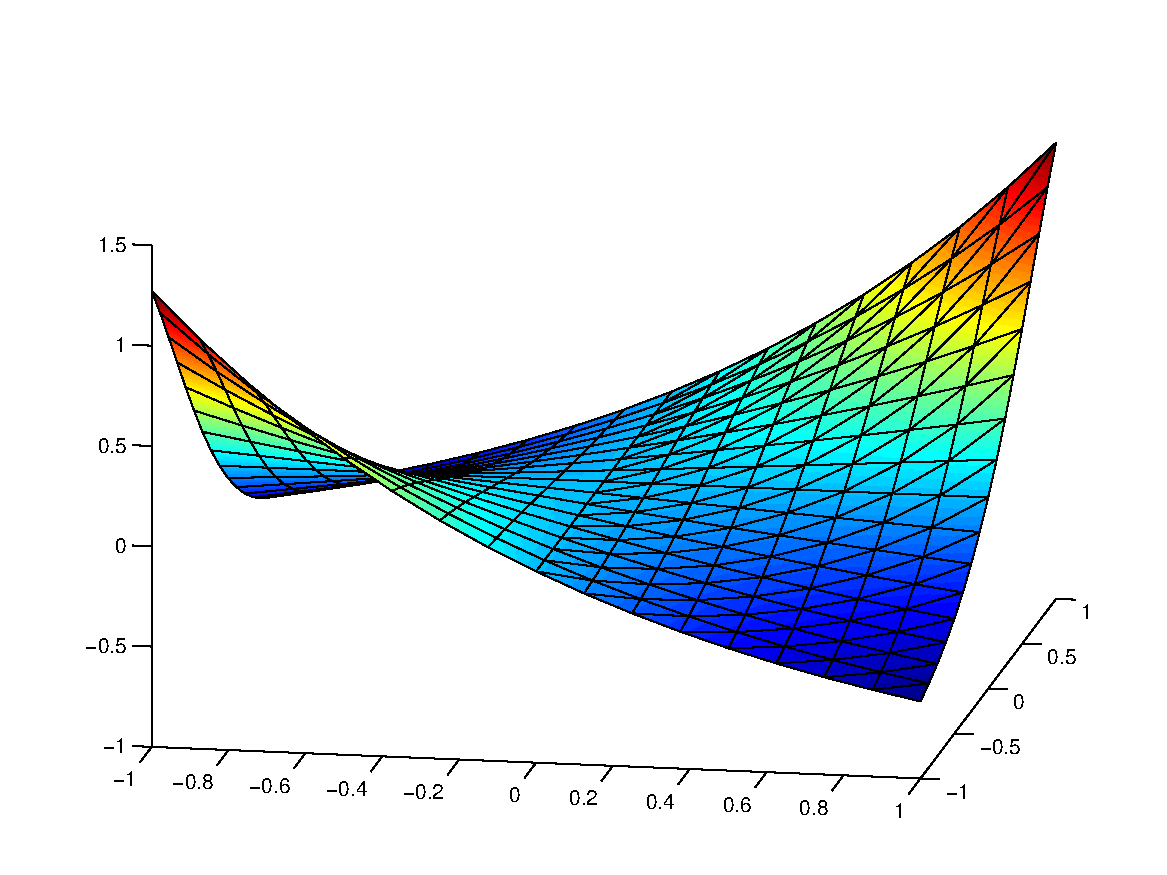
\includegraphics[height=0.27\textheight]{plots/poissonHybrid/phicubic16x16.pdf}\\
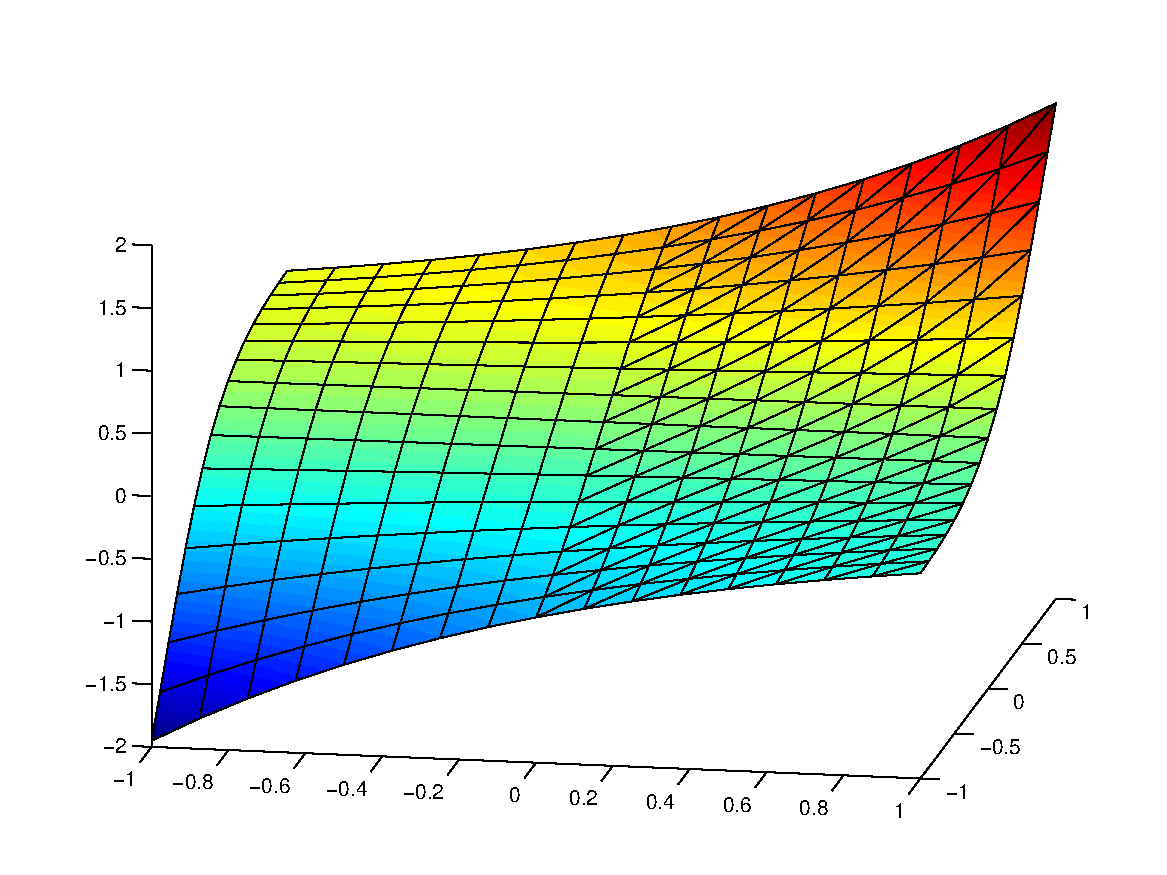
\includegraphics[height=0.27\textheight]{plots/poissonHybrid/psi1cubic16x16.pdf}\\
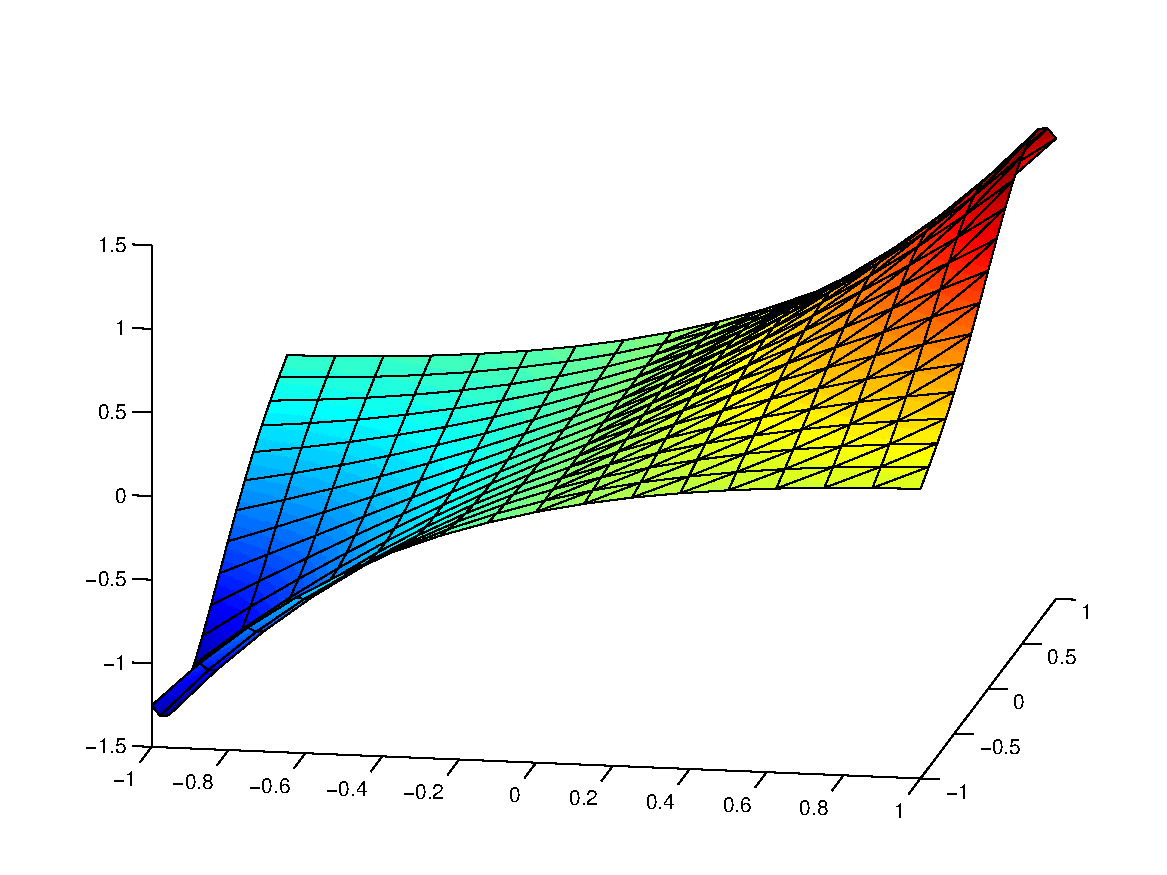
\includegraphics[height=0.27\textheight]{plots/poissonHybrid/psi2cubic16x16.pdf}
\caption{Solution of Poisson with quads and triangles (cubic elements, $16 \times 16$ mesh):
$\phi$ (top pane),
$\psi_{1}$ (middle pane)
$\psi_{2}$ (bottom pane).}
\label{NVR:fig:Poisson}
\end{center}\end{figure}

\begin{figure}[h!b!h!]
\begin{center}
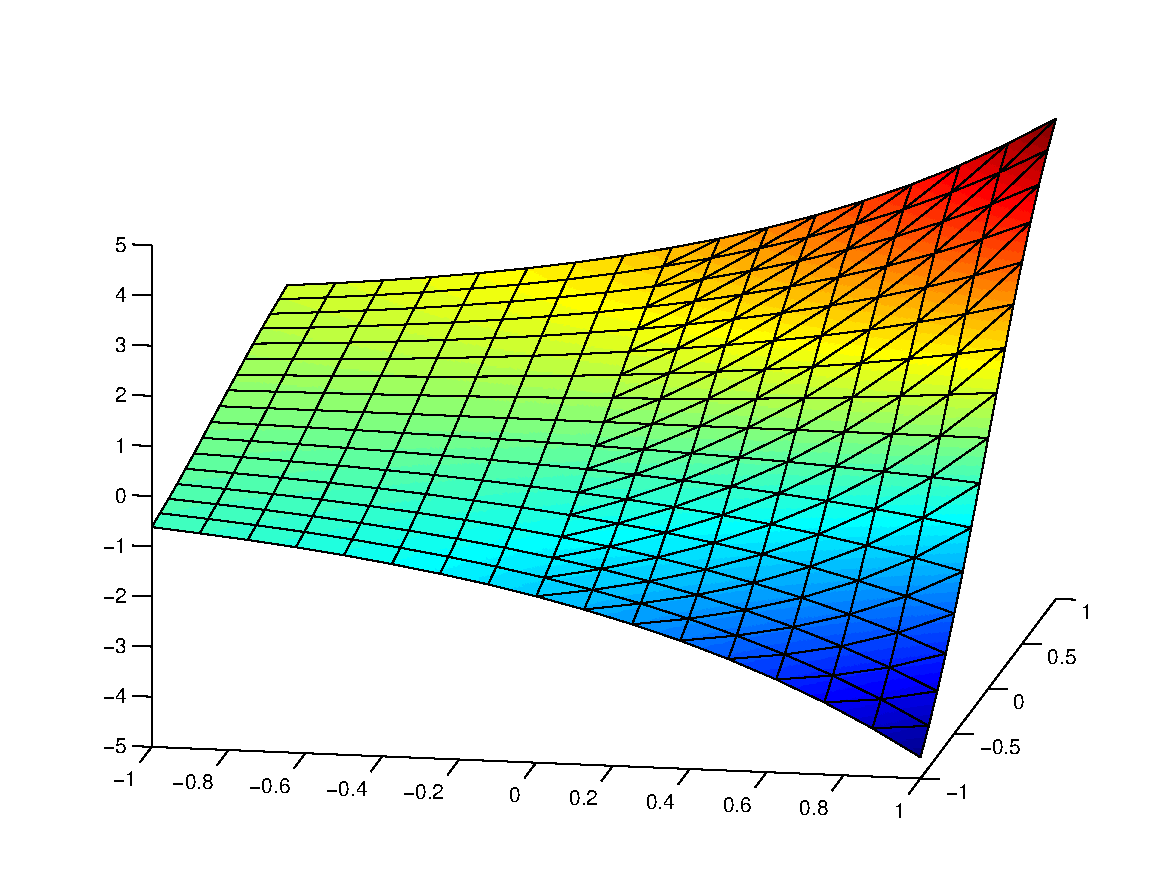
\includegraphics[height=0.27\textheight]{plots/stokesVVPHybrid/pressurecubic16x16.pdf}
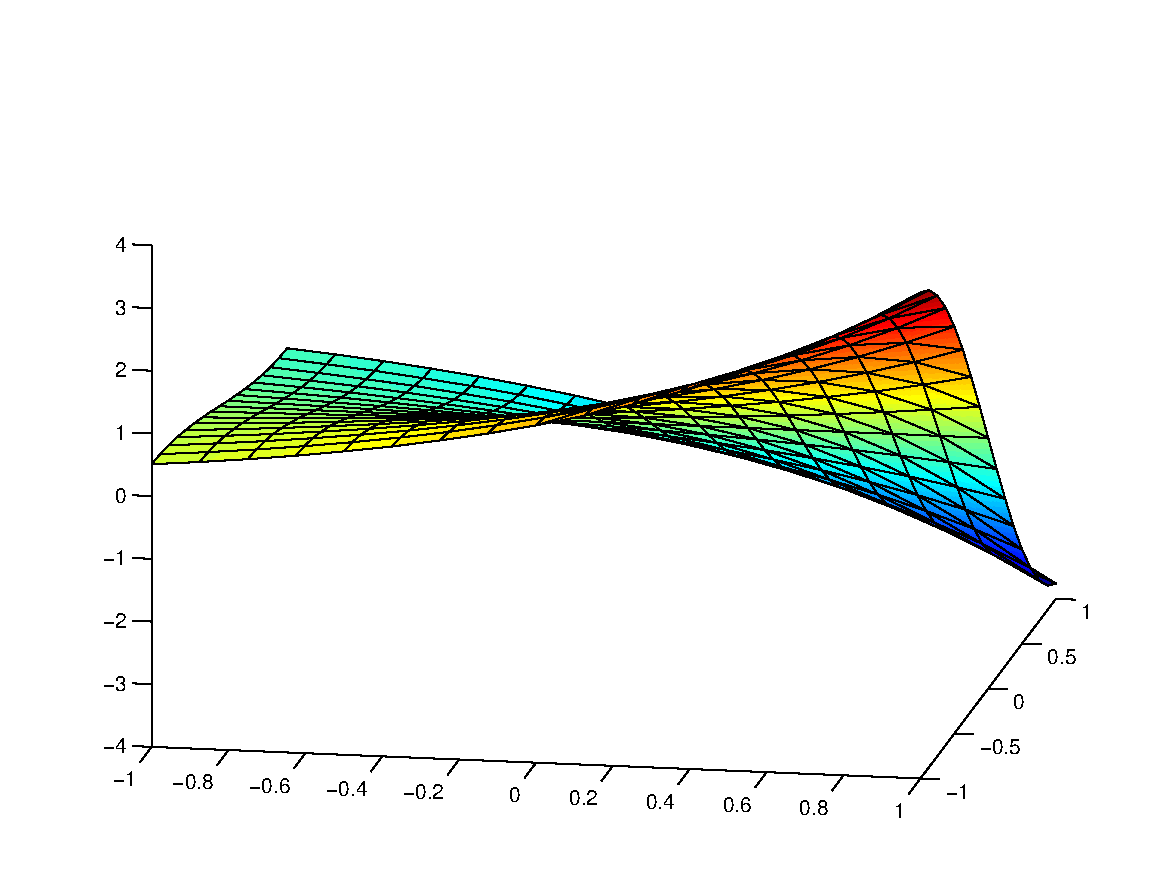
\includegraphics[height=0.27\textheight]{plots/stokesVVPHybrid/u1cubic16x16.pdf}
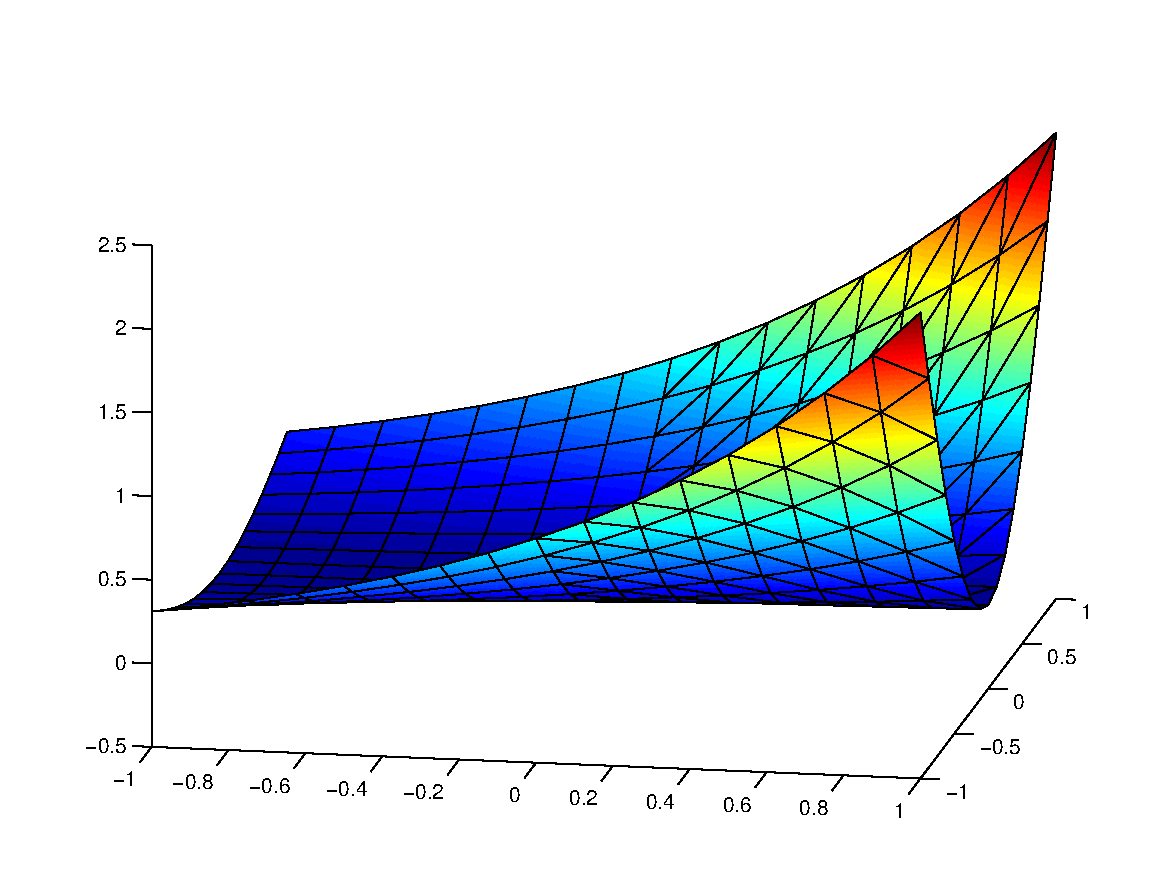
\includegraphics[height=0.27\textheight]{plots/stokesVVPHybrid/u2cubic16x16.pdf}
\caption{Solution of Stokes (VVP) with quads and triangles (cubic elements, $16 \times 16$ mesh):
$p$ (top pane),
$u_{1}$ (middle pane),
$u_{2}$ (bottom pane).}
\label{NVR:fig:Stokes}
\end{center}\end{figure}

\clearpage

\subsection{Extending Camellia for Distributed Stiffness Matrix Determination}\label{sec:distributingStiffness}
Here, we describe the changes that we implemented within Camellia to allow the stiffness matrix determination to be executed efficiently within an MPI environment.

Camellia was originally written to run in serial, so a number of changes were required to allow MPI execution---the most significant of these had to do with element partitioning and partitioning the degree-of-freedom coefficients.  Trilinos's Intrepid routines are designed to execute on batches of cells that are alike in topology and polynomial order.  We allow meshes of non-uniform topology and polynomial order; thus we had implemented an ElementType class which allowed us to identify elements that could be batched.  Our Mesh class maintained data structures such that information pertaining to a particular ElementType could be accessed quickly---for example, Mesh stored a data structure that contained the vertex coordinates belonging to elements of a given ElementType.

The upshot of this design is that mesh information is already, in a sense, partitioned.  However, there is no reason to expect that this will be a good partitioning for dividing up the work of stiffness matrix computation across MPI nodes---for this, we want our mesh partitioning to keep spatially adjacent elements together within a partition to minimize the amount of data that needs to be communicated during global stiffness matrix assembly.

Thus, to maintain both of our desired design features---batching by ElementType and spatially contiguous partitioning across MPI nodes---we require a two-level partitioning; we first divide the elements spatially (the MPI partitions), and then batch together elements of like ElementType within each of these partitions.  (Unfortunately, this is not quite the whole story; because other classes depend on the ElementType division of the whole mesh, we have had to maintain the old lookup tables as well.  We do hope to eliminate these dependencies in the end.)

To facilitate experiments with multiple partitioning strategies (and to maintain separation of concerns), we designed an abstract MeshPartitionPolicy class which, given a Mesh and the number of partitions desired, returns a partition of the elements in the mesh.  The Mesh then uses this to generate a partition of the degree-of-freedom coefficients, which induces a partition of the rows in the stiffness matrix.  The latter partition is used in conjunction with an Epetra FECrsMatrix, a distributed stiffness matrix class within Trilinos.  The FECrsMatrix allows storage of data not owned by the current MPI node; this data is communicated to the owning MPI node during global assembly of the stiffness matrix.  A convenient consequence of this is that we can separate the cost of global assembly from the cost of local stiffness matrix computations; the latter are independent across MPI nodes, and therefore we expect to see perfect scaling for these.  The scaling of the global assembly will depend on the quality of the partition and the cost of communication between MPI nodes.  We do not hope for perfect scaling here, but we do hope to see a cost per degree of freedom per node that does not grow too quickly in the total number of nodes.

The MeshPartitionPolicy partitions the mesh into sets of elements assigned to an MPI node; for the interface to Epetra, we need a partition of rows of the global stiffness matrix (each of which corresponds to a degree of freedom).  Degrees of freedom corresponding to numerical fluxes are shared by the elements along whose boundaries they lie.  We adopt a simple greedy policy for assignment of these d.o.f.s: shared d.o.f.s are assigned to the element with the smallest global identifier.  This means that even if the element partitioning were perfectly balanced, some MPI nodes might still have more d.o.f.s assigned to them than others.  This will not affect the amount of work involved in local stiffness matrix computations, but it may affect MPI communication costs during global assembly.

\paragraph{Design Limitations: where Amdahl's law might come to haunt us.}
Here, we note a few features of the present design that may become bottlenecks as we scale up to larger problems and larger numbers of MPI nodes.

At present, our global solve is implemented using the KLU implementation provided by the Amesos package within Trilinos.  This is a direct solve, executed in serial.  Amesos gathers the global stiffness matrix to rank 0, solves, and then scatters the solution according to the partition we have defined.  For our serial computations prior to the present work, the cost of the global solve has been dominated by the cost of the local optimal test function determination; however, now that the latter cost has been distributed using MPI and the former has not, we expect the global solve to become a bottleneck, both in terms of overall execution time and in terms of the sizes of problems that can be solved, since the KLU solve must fit into a single node's memory to be practical.

Similarly, at present the entire mesh is determined and stored on every MPI node.  This has the advantage that no MPI communication is required during mesh construction, but for very large meshes it may become impractical, because the time cost of mesh construction may grow relative to the distributed parts of the computation, and perhaps (for \emph{extremely} large meshes) because the memory required for the mesh may grow too large for storage on a node.

Finally, certain features of the original code depend upon all the solution coefficients being available to the current processor, so for the time being we distribute the entire solution to every MPI node, after Amesos has scattered according to the original partitioning.  We hope to eliminate this dependence on having all solution coefficients available, allowing the solution to be distributed according to the same mapping as was used for the stiffness matrix.

\subsubsection{Partitioning}

Since Camellia is tightly integrated with the Trilinos library already, we use the Zoltan package in Trilinos to generate spatially local partitions of the mesh \cite{ZoltanOverviewArticle}. We interface specifically with the Hilbert Space-filling Curve and Reftree partitioning algorithms in Zoltan, both of which can include parallel implementations. 

The Hilbert space-filling curve (HSFC) algorithm works by drawing a curve through the geometric mesh in 2- or 3-dimensional space, then mapping that curve to the interval $[0,1]$. The partitioner then divides up this interval (in an even or weighted manner) into $n$ partitions, and uses this partitioning to induce a partition of the mesh. All that's required by the HSFC algorithm is a listing of elements and a geometric identifier associated with a given element. In this case, we use the element centroid as such an identifier. 

The Reftree algorithm \cite{REFTREE} adds complexity in that each processor must store information not only about the active nodes, but the ancestors as well. Reftree also requires that if you store an ancestor, you also store all its children as well, increasing the amount of redundancy between distributed refinement trees. However, since Reftree is not tuned to a particular element types (quad or triangle, tetrahedron or cube), the same algorithm performs similarly for many different types of refined meshes (as opposed to HSFC, which works best for quadrilateral grids, but not for triangular grids).  Additionally, Reftree's algorithm guarantees connected partitions for tetrahedral and triangular grids, and generally performs more robustly on other types of grids as well.

Currently, we have implemented and tested a Reftree MeshPartitionPolicy on our workstations. However, Reftree currently crashes during runs on Lonestar, our HPC architecture for this report. We used the HSFC partitioner for the scaling tests in this report, and hope to fix issues with Reftree in the near future. 

\subsubsection{Scaling tests}\label{sec:ScalingExperiments}

We tested the scalability of our code on the Lonestar machine at the Texas Advanced Computing Center (TACC), verifying whether or not we observe strong/weak scaling for various parts of the program.  We solve the convection-diffusion equation on a square mesh, with boundary conditions such that the solution develops a boundary layer (sharp gradient) near the north and east edges of the square.  The solution for a refined mesh is shown in Figure \ref{fig:solutionPlot}.

\begin{figure}[h!]
\centering
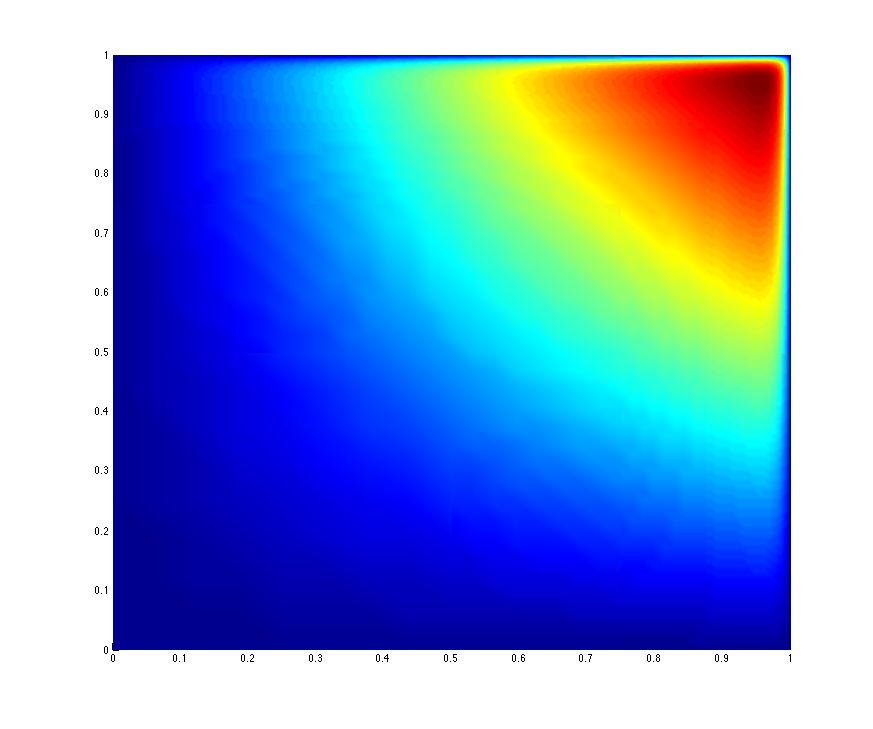
\includegraphics[scale=0.45]{figs/Solution12928nomesh.png}
\caption{Computed solution for $\epsilon=10^{-2}$ using a 12,928-element mesh.  $L^2$ error is $O(10^{-5})$.}
\label{fig:solutionPlot}
\end{figure}

We set up our computational experiments by first refining all cells that share an edge with the north and east sides, and repeating this process four times.   We then constructed three additional meshes, by uniformly refining every element in the mesh (quadrupling the number of elements each time).  For each of these meshes, we solved on Lonestar, using 1, 4, 16, and 64 nodes, tracking the timing of various portions of the code.  From this data, we extracted strong and weak scaling statistics, discussed below in Sections \ref{sec:strongScaling} and \ref{sec:weakScaling}.  The runtimes plotted in each of our figures are the mean of the times recorded at each MPI node.

We also used contiguous and discontiguous partitions of each mesh to measure the effect of partition quality on the communication costs in global stiffness matrix assembly.  We created contiguous partitions of the mesh using a HSFC partitioner.  To create the discontiguous partitioning, we used the Zoltan cyclic partitioner, which loops through the list of active elements, sending the first element to the first processor, the next to the next processor, and so on.  After reaching the last processor, the cyclic partitioner cycles back to the first processor and repeats this process.\footnote{Due to the nature of our refinements in this test, a blocked partitioner (equally partitioning the ordered list of active elements by element number) happened to produce nearly-contiguous partitions.  We therefore have omitted this partitioner from our analysis, since we do not believe that its performance here accurately predicts its performance in general.}  The cyclic partitioning is a ``worst case" scenario in the sense that each of the current MPI node's elements' neighbors are owned by some other MPI node, with the consequence that information concerning each element boundary must be sent via MPI.  An example cyclic partitioning can be seen in Figure \ref{fig:cyclicPartition}; Figure \ref{fig:HSFCPartition} shows an HSFC partitioning.

It's worth noting that the runtimes reported here do not represent Camellia running at peak efficiency.  A single Lonestar node contains 12 cores.  Because MPI communication has much higher bandwidth intra-node than inter-node, and for analysis we wanted approximately equal bandwidth between MPI processes, we use only one core per node.  Utilizing all 12 cores on a node would decrease communication costs.  Additionally, there is a parameter within Camellia that controls the batch size for the Trilinos Intrepid batching routines.  Tuning this parameter based on machine-specific cache sizes should further improve performance.

\begin{figure}[h!]
\centering
\subfigure[Cyclic partitioning]{\label{fig:cyclicPartition}
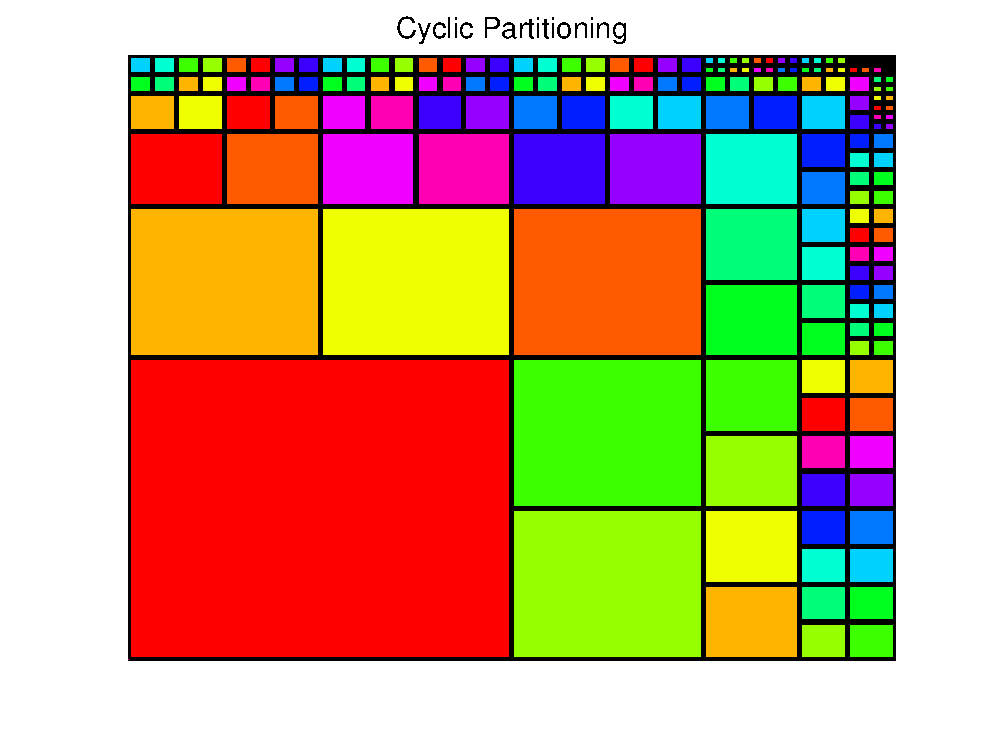
\includegraphics[scale = 0.42]{figs/cyclic.pdf}
}
\subfigure[HSFC partitioning]{\label{fig:HSFCPartition}
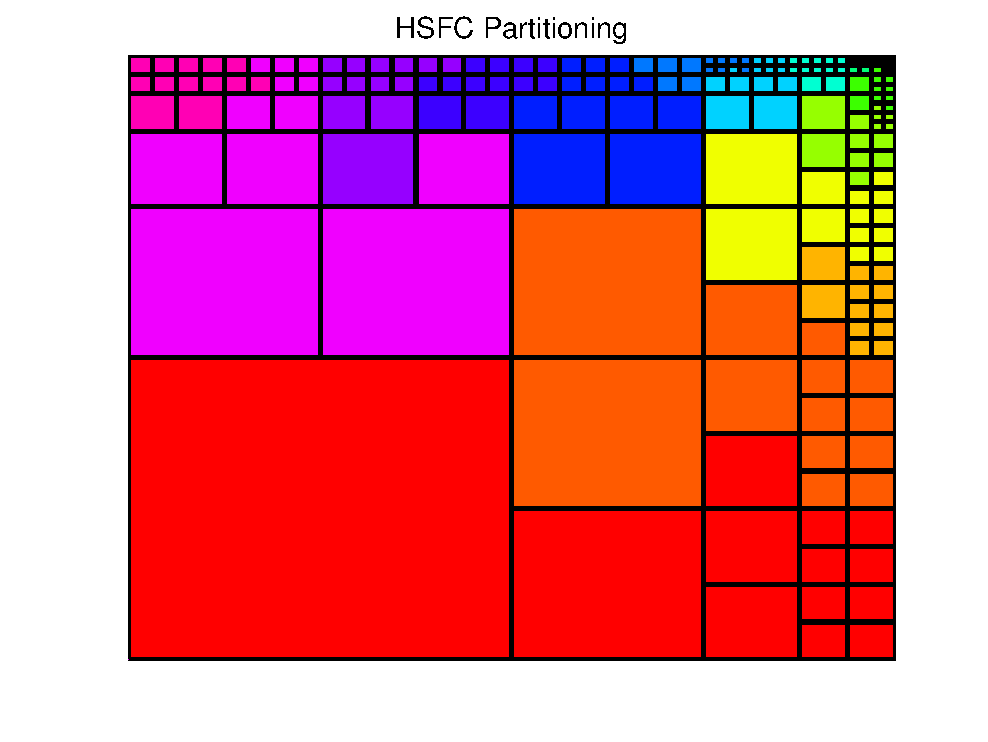
\includegraphics[scale = 0.42]{figs/hsfc.pdf}
}
\caption{Discontiguous and contiguous partitions of the mesh.}
\end{figure}

\subsubsection{Strong scaling}\label{sec:strongScaling}
In our strong scaling tests, we considered problems of fixed size, distributing the workload for each among increasing numbers of MPI nodes.  Here, we hope to see runtimes that decrease linearly in the number of MPI nodes---this is what we mean by achieving strong scalability.

Because the local stiffness computations are entirely independent of each other, requiring no communication among MPI nodes, we expect to see perfect scaling for these.  As can be seen in Figures \ref{fig:strongScalingLocalStiffnessCyclic} and \ref{fig:strongScalingLocalStiffnessHSFC}, we do achieve something very close to this, although the cyclic partitioning took longer in almost every case, for reasons that are unclear to us.  It may have something to do with data locality on each node---by the manner of our construction, data concerning contiguous mesh elements is more likely to be close together in memory than the data for mesh elements in the cyclic case.

It is less clear what we should expect for the global stiffness matrix assembly; we expect the HSFC partitioning to outperform the cyclic partitioning, and we would like to see the runtimes for assembly decrease as the number of MPI nodes increases.  As can be seen in Figures \ref{fig:strongScalingAssemblyCyclic} and \ref{fig:strongScalingAssemblyHSFC}, for the larger problems in both cases, we do have something approaching strong scalability.  For the 202- and 808-element problems, we see the time cost increase (or fail to decrease, in the case of the 808-element problem for the cyclic partitioner) between 16 and 64 nodes.  However, it's worth noting that in these cases, the real times involved are small: less than a second in each case.  If our concern is our ability to scale up to large problems on large numbers of processors, it does not appear that the global assembly will be a bottleneck.  The HSFC partitioning does show its strength here compared with the cyclic; for the 12,928 mesh on the 4-node run, the cyclic partitioning took an average of 49.1 seconds per node, compared with 1.63 seconds for the HSFC partitioning.

\begin{figure}[h!]
\centering
\subfigure[Cyclic Partitioning]{\label{fig:strongScalingLocalStiffnessCyclic}
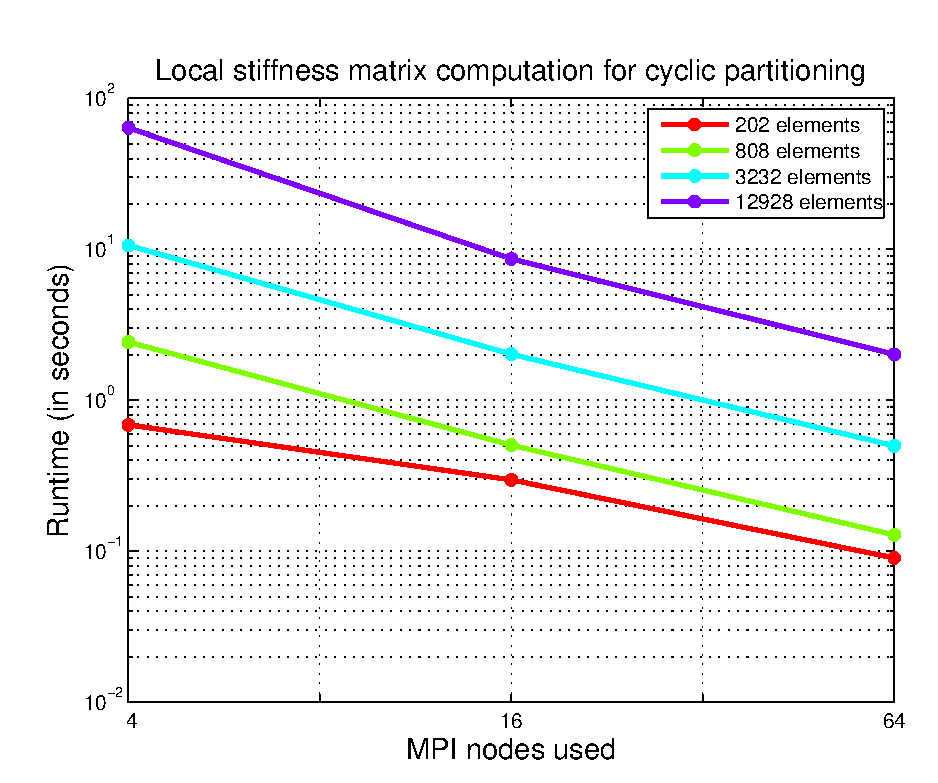
\includegraphics[scale = 0.42]{figs/scalingFigs/cyclicStrongScalingLocal.pdf}
}
\subfigure[HSFC Partitioning]{\label{fig:strongScalingLocalStiffnessHSFC}
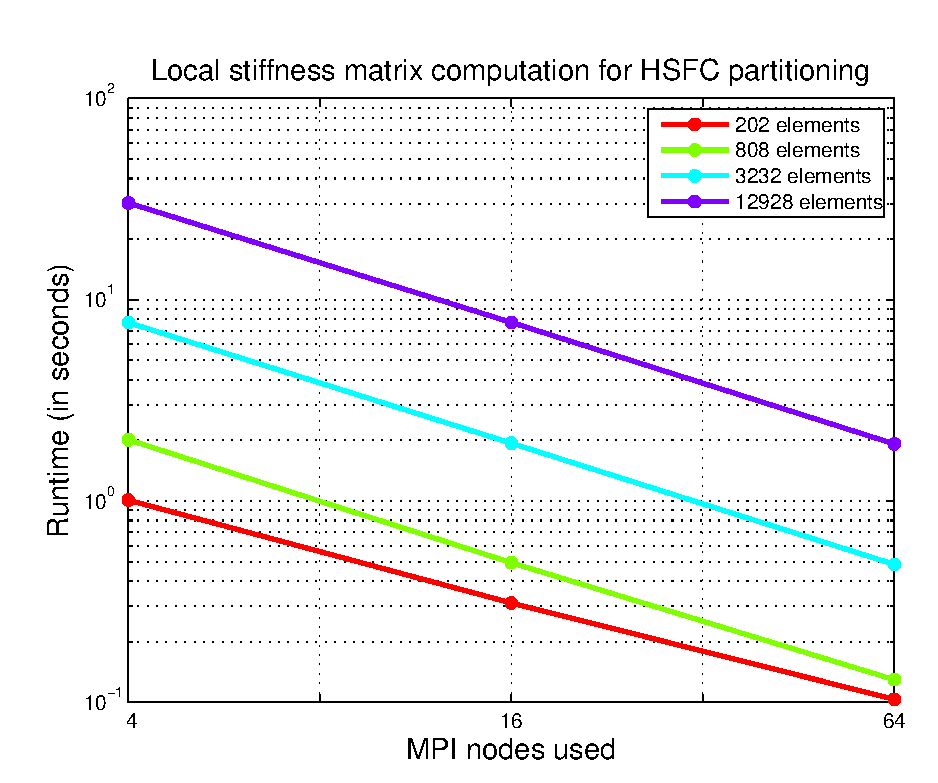
\includegraphics[scale = 0.42]{figs/scalingFigs/hsfcStrongScalingLocal.pdf}
}
\caption{Strong scaling plots for the local stiffness matrix computation.}
\end{figure}

\begin{figure}[h!]
\centering
\subfigure[Cyclic Partitioning]{\label{fig:strongScalingAssemblyCyclic}
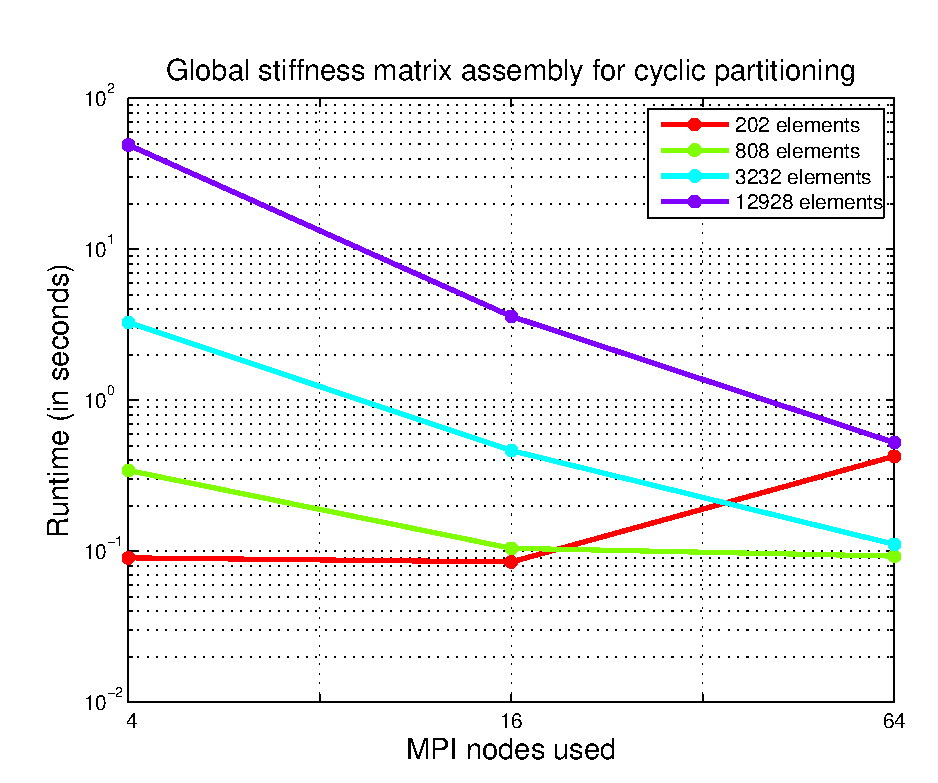
\includegraphics[scale = 0.42]{figs/scalingFigs/cyclicStrongScalingAssembly.pdf}
}
\subfigure[HSFC Partitioning]{\label{fig:strongScalingAssemblyHSFC}
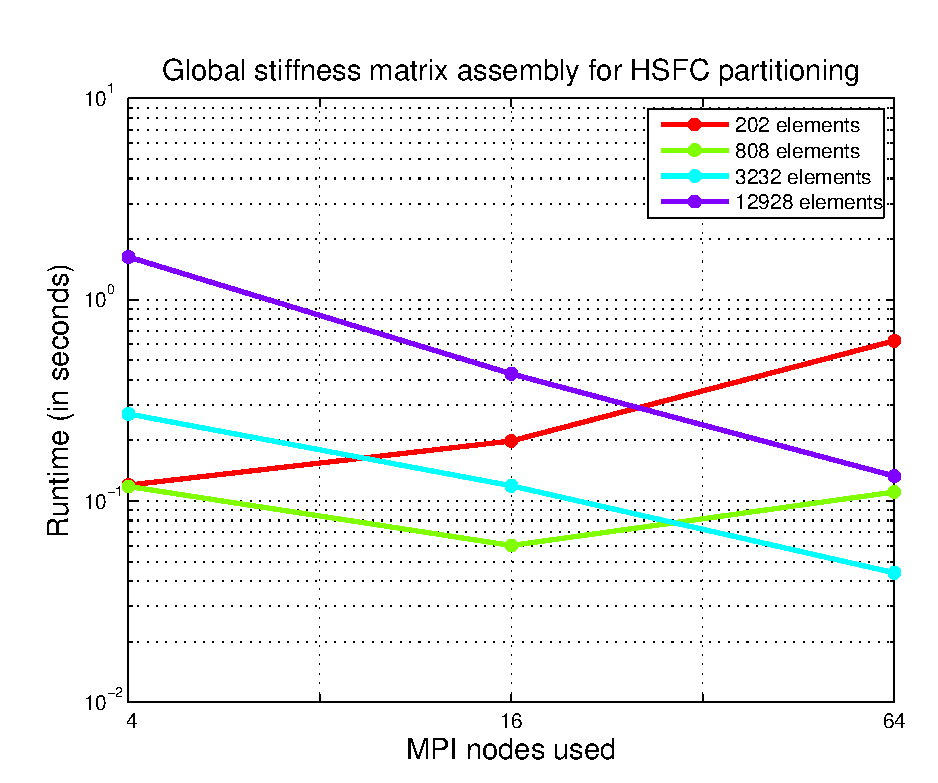
\includegraphics[scale = 0.42]{figs/scalingFigs/hsfcStrongScalingAssembly.pdf}
}
\caption{Strong scaling plots for global stiffness matrix assembly.  (Note the differing scales.) }
\end{figure}

\subsubsection{Weak scaling}\label{sec:weakScaling}
In our weak scaling tests, we aimed to fix the size of the problem \emph{per MPI node}, and examined the runtime of various portions of the execution---we hope to see a constant runtime as the problem size and number of processors increase, and this is what we mean by achieving weak scalability.

\begin{figure}[h!]
\centering
\subfigure[Local stiffness computation]{
\label{fig:weakScalingStiffness}
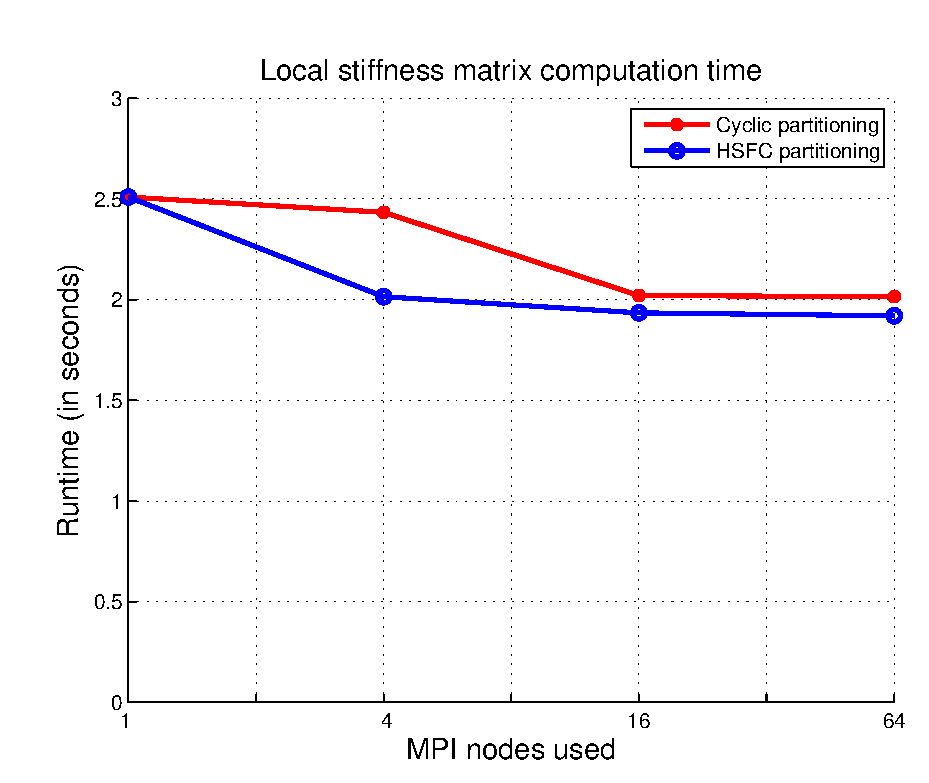
\includegraphics[scale = 0.42]{figs/scalingFigs/weakScalingLocal.pdf}
}
\subfigure[Global stiffness assembly]{
\label{fig:weakScalingAssembly}
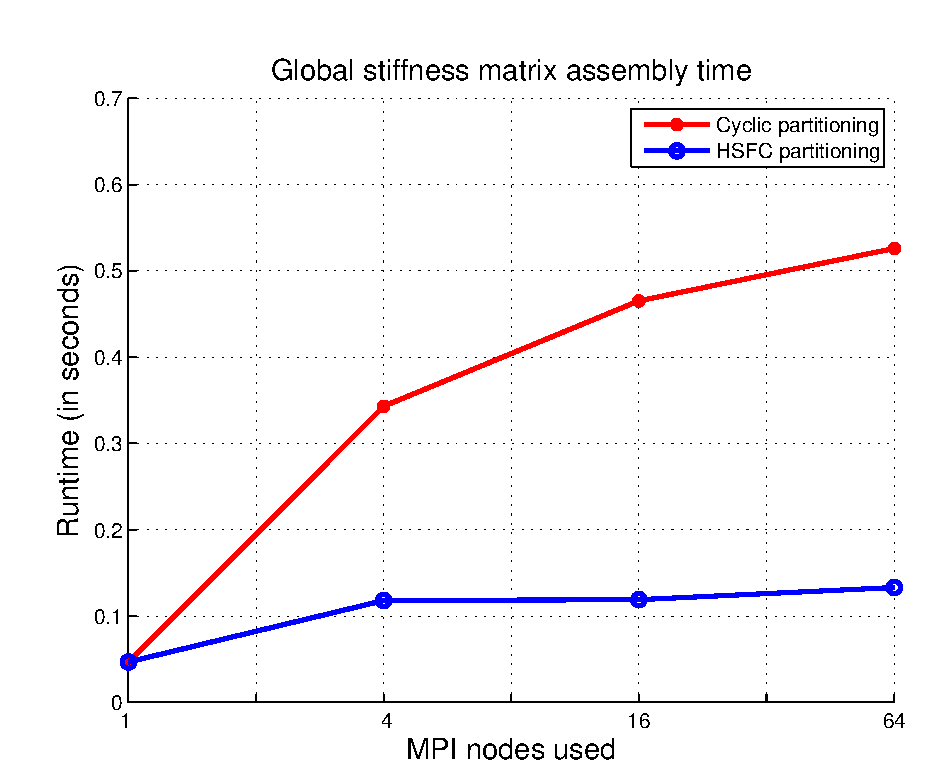
\includegraphics[scale = 0.42]{figs/scalingFigs/weakScalingAssembly.pdf}
}
\caption{Weak scaling results for computation of local stiffness matrices and global stiffness matrix assembly.  For each run, both the number of MPI nodes and the number of elements increased by a factor of four.}
\end{figure}

Both partition types achieve weak scalability in the local stiffness matrix computation, as can be seen in Figure \ref{fig:weakScalingStiffness}.  In fact, we see the total runtime \emph{decrease} slightly as the total workload and number of MPI nodes increase---we are unsure of the reason for this. Although we would not expect the partitioning to affect this portion of the computation at all (since no inter-node communication occurs at this stage), for some reason the HSFC partitioning slightly outperforms the cyclic on each of the multi-node runs.  As with the strong scaling, we speculate that this is due to locality of the owned element data in the case of the HSFC partitioning.

Assembly of the global stiffness matrix achieves weak scalability only for the contiguous case, as can be seen in Figure \ref{fig:weakScalingAssembly}. It's worth noting, however, that though the poor mesh partitioning imposes much higher communication costs than the HSFC partitioning, the maximum amount of time spent on assembly is still dominated by the time spent on computation of local stiffness matrices.

\subsubsection{Total runtime analysis}\label{sec:runtimeAnalysis}
As the final component of our performance analysis, we examine components of the total runtime for each of our four problems using 1, 4, 16, and 64 MPI nodes; here we use the HSFC partitioner.  This can be seen in Figure \ref{fig:timeBreakdown}.  We see that for the largest MPI runs the combined time spent on local stiffness computation and global assembly is a small fraction of the total time spent---since these were the targets of the present work, we can count it a success.  The graphs also show that the cost of the global solve dominates in each of these runs, making this the obvious next target for optimization.  In the ``Other'' category, the largest cost is the mesh determination.  In the 12,928-element case, this takes about 5 seconds.  Thus, a distributed mesh might be our next target after the solve is optimized.

\begin{figure}[h!]
\centering
\subfigure[202 elements, 13,343 dofs]{
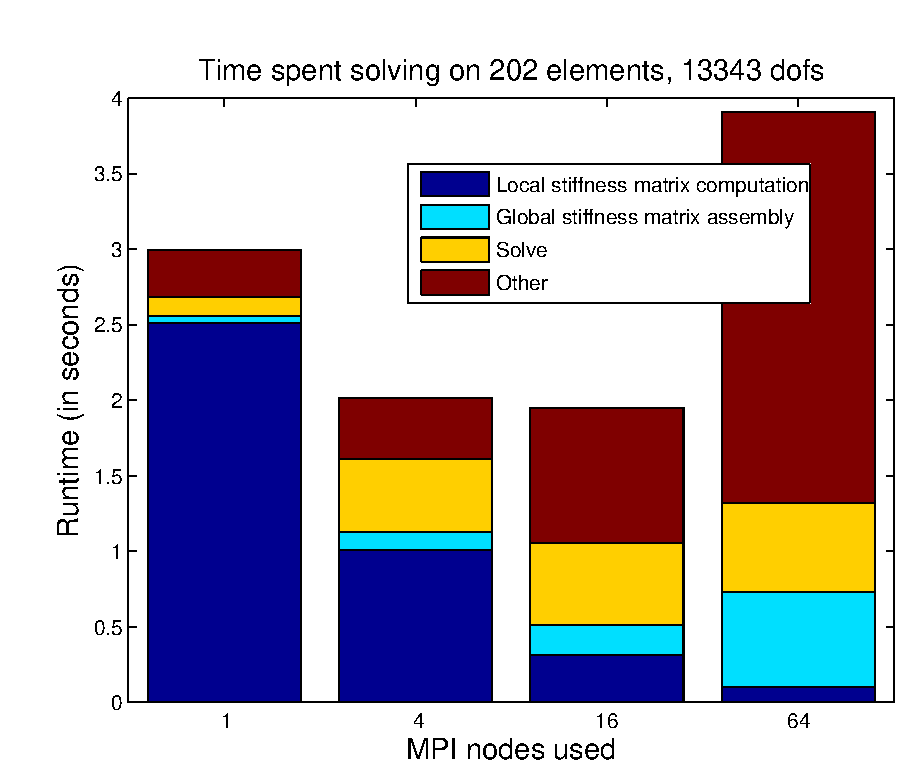
\includegraphics[scale = 0.42]{figs/scalingFigs/bar_ref0.pdf}
}
\subfigure[808 elements, 52,137 dofs ]{
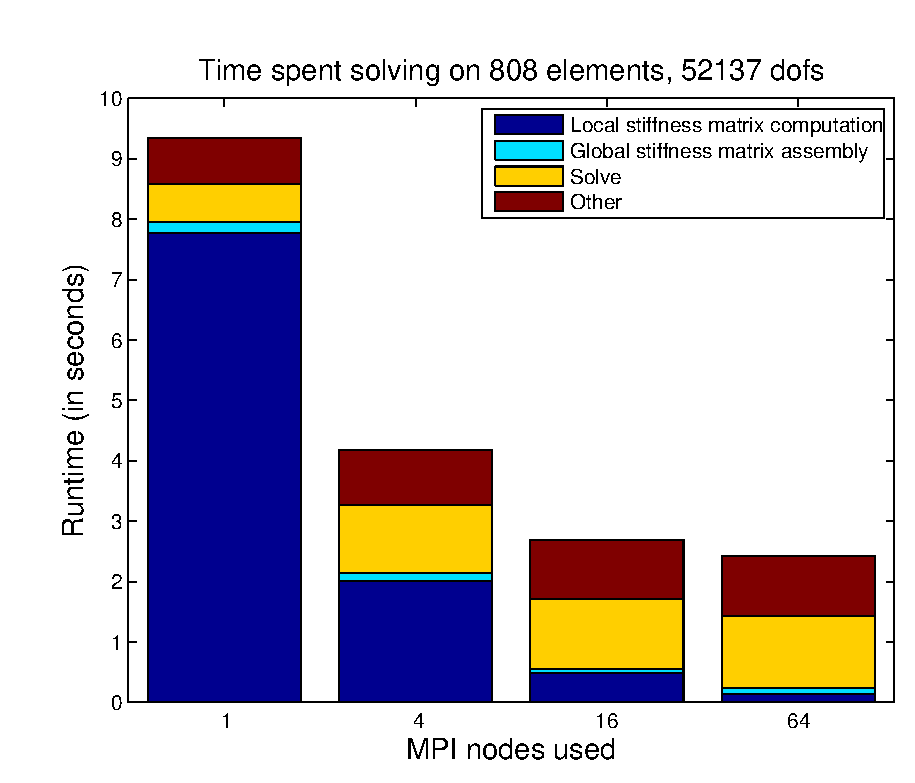
\includegraphics[scale = 0.42]{figs/scalingFigs/bar_ref1.pdf}
}
\subfigure[3,232 elements, 206,081 dofs]{
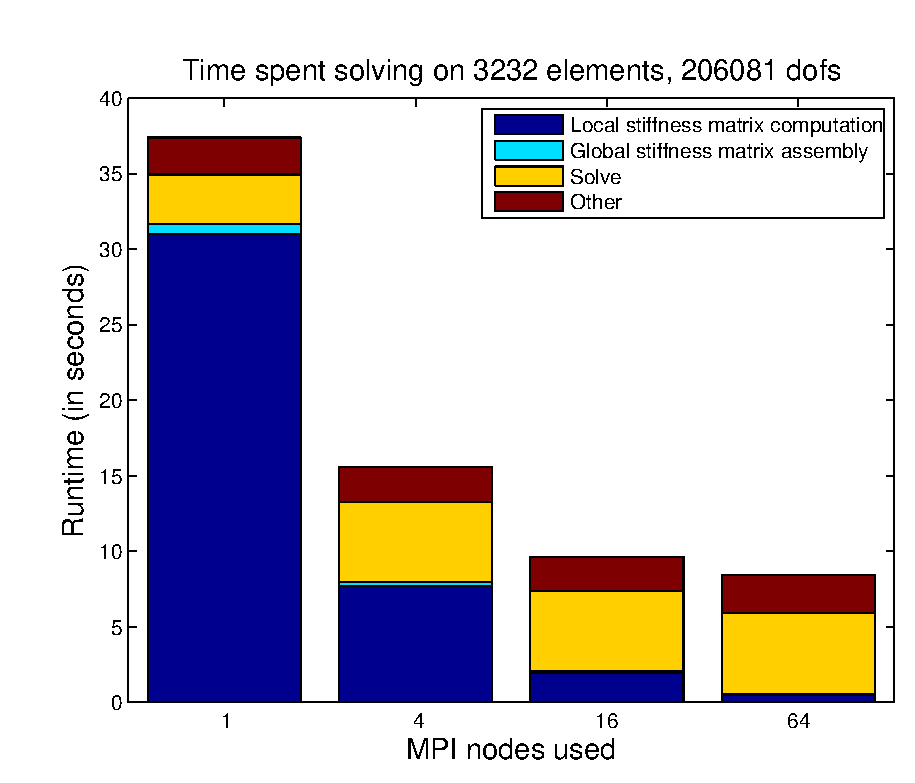
\includegraphics[scale = 0.42]{figs/scalingFigs/bar_ref2.pdf}
}
\subfigure[12,928 elements, 819,393 dofs]{
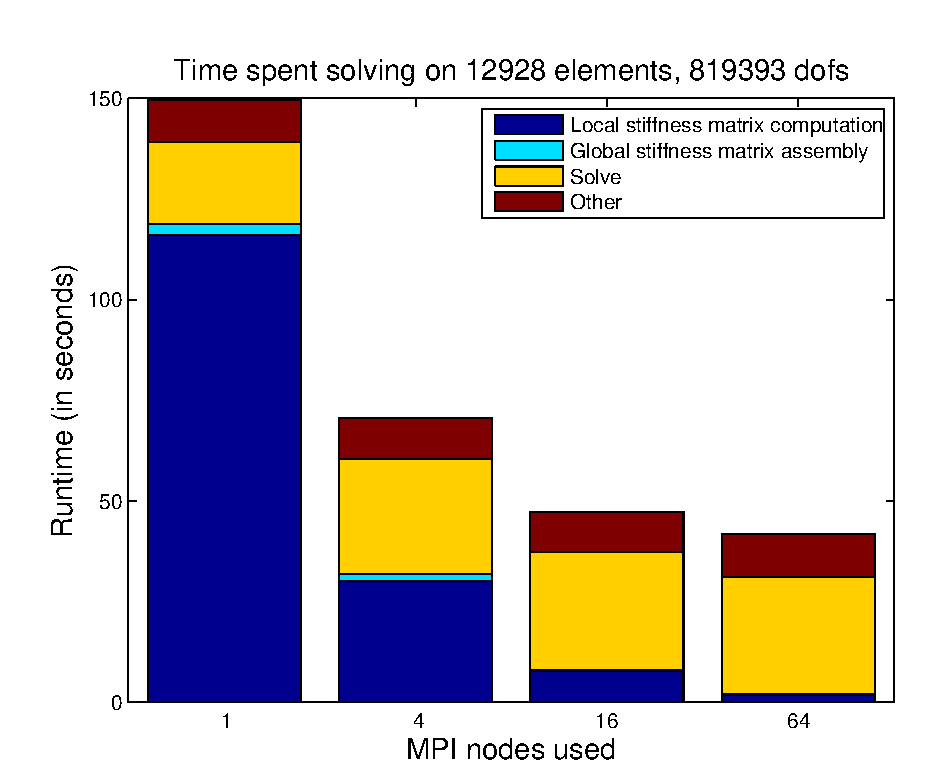
\includegraphics[scale = 0.42]{figs/scalingFigs/bar_ref3.pdf}
}
\caption{Breakdown of time spent in a solve for a series of HSFC-partitioned meshes.}
\label{fig:timeBreakdown}
\end{figure}

\subsubsection{Future Work for Better Scaling}\label{sec:FutureWork}
There are several ways in which we hope to extend Camellia further to allow it to solve larger problems still; we hope to:
\begin{itemize}
\item distribute the solve, using MUMPS or an iterative solver,
\item improve the load balancing for meshes of variable polynomial order,
\item distribute mesh construction and storage, and
\item distribute solution storage.
\end{itemize}

As discussed in Section \ref{sec:runtimeAnalysis} above, the lowest-hanging fruit for further improving the performance for the experimental setup considered in the present work is distributing the solve.  We have already successfully interfaced with MUMPS---a parallel sparse direct solver---on one of our laptops; we expect that getting MUMPS to work on Lonestar will just be a matter of building Trilinos and Camellia with MUMPS there.  One of the advantages of DPG is that its stiffness matrices are guaranteed to be symmetric positive definite, which opens the door to using iterative methods such as conjugate gradient methods.  DPG also produces matrices whose entries are coupled only through the flux degrees of freedom; thus static condensation techniques can be used to reduce the size of the global system to be solved.  We believe that iterative solvers and static condensation would allow us to solve larger problems than MUMPS will allow---we have heard that MUMPS only scales to about 128 processors.

In the present work, we considered a mesh of uniform polynomial order and considered all elements to be of equal weight; Camellia supports meshes with variable order, and Zoltan provides facilities for weighting elements differently.  By taking advantage of this feature of Zoltan (using a weight corresponding to the number of degrees of freedom on each element), we can improve Camellia's load balancing for meshes of variable polynomial order.  In fact, in doing so, we expect to improve slightly the load balancing for the setup considered here, because elements with hanging nodes do have slightly more degrees of freedom than those without.

At present, the mesh is constructed and stored on each node, as is the solution.  It should be a relatively small extension to the present work to allow the solution to be distributed.  Allowing mesh construction to be distributed is a bigger challenge, largely because the nodes must agree on the global stiffness matrix row indices.  Given that we are working with an adaptive mesh, it will likely make sense to distribute the work of mesh refinement according to the partition of the previous mesh and use Zoltan to do the load rebalancing.

In summary, we have achieved good overall speedup for Camellia using a Hilbert space-filling curve partitioner, and have identified the next steps for improving its parallel performance further.

\subsection{Demonstration of Nonlinear Solution Capabilities: Compressible Navier-Stokes}\label{sec:compressibleNS}
Jesse Chan has applied Camellia's nonlinear solve capabilities to the compressible Navier-Stokes equations in the context of Carter's flat plate problem.  We include here some plots that demonstrate the success of the adaptive mesh (Figure \ref{fig:JCmeshRefinements}), as well as a plot of the final solution for the velocity in the $x$ direction (Figure \ref{fig:JCu1}).  This experiment was performed with a Reynolds number of 1000 and a Mach number of 3.

\begin{figure}[h!]
\centering
\subfigure[i=0]{
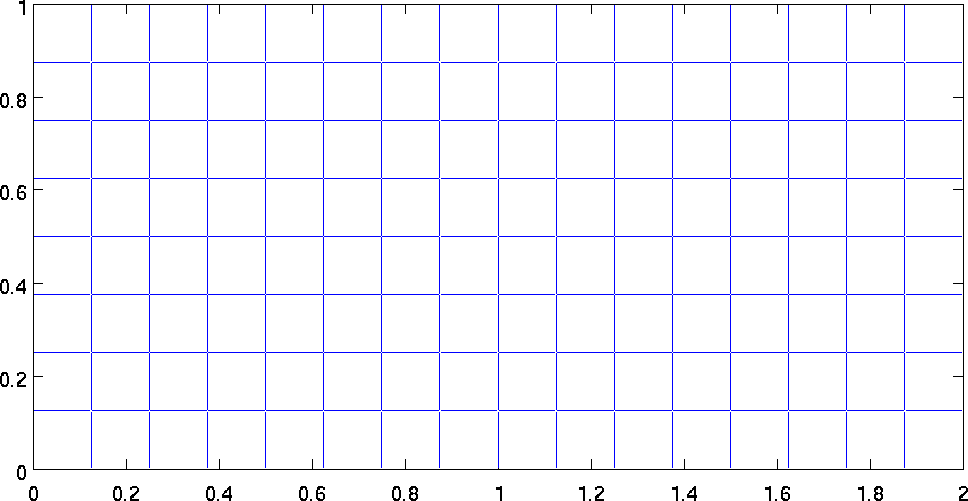
\includegraphics[scale = 0.45]{figures/mesh0.png}
}
\subfigure[i=1]{
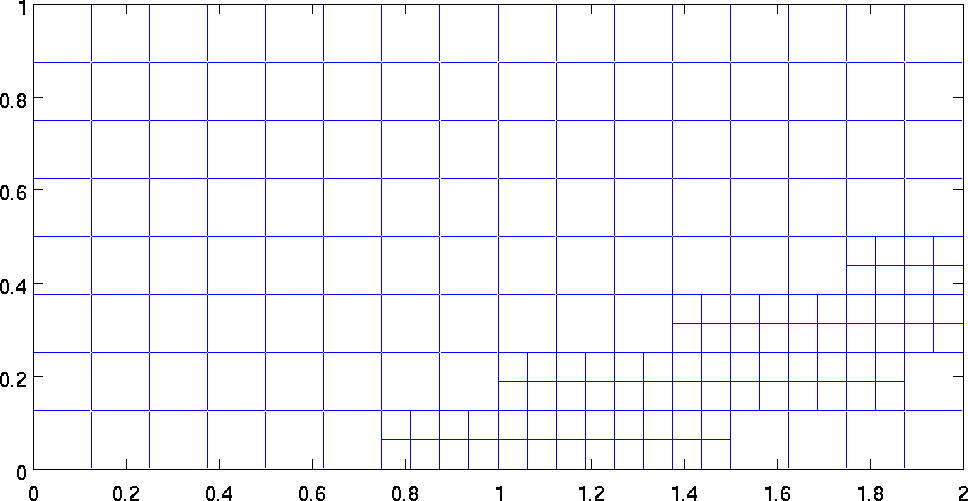
\includegraphics[scale = 0.45]{figures/mesh1.png}
}
\subfigure[i=2]{
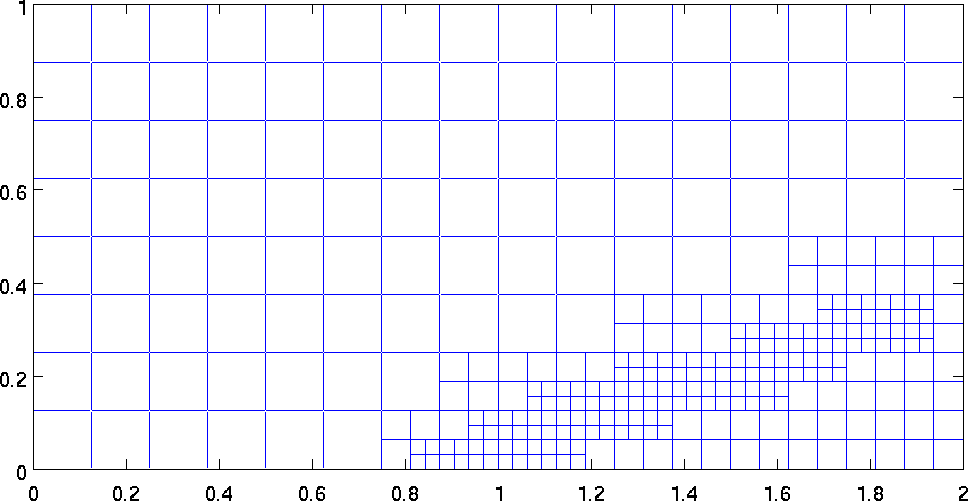
\includegraphics[scale = 0.45]{figures/mesh2.png}
}
\subfigure[i=4]{
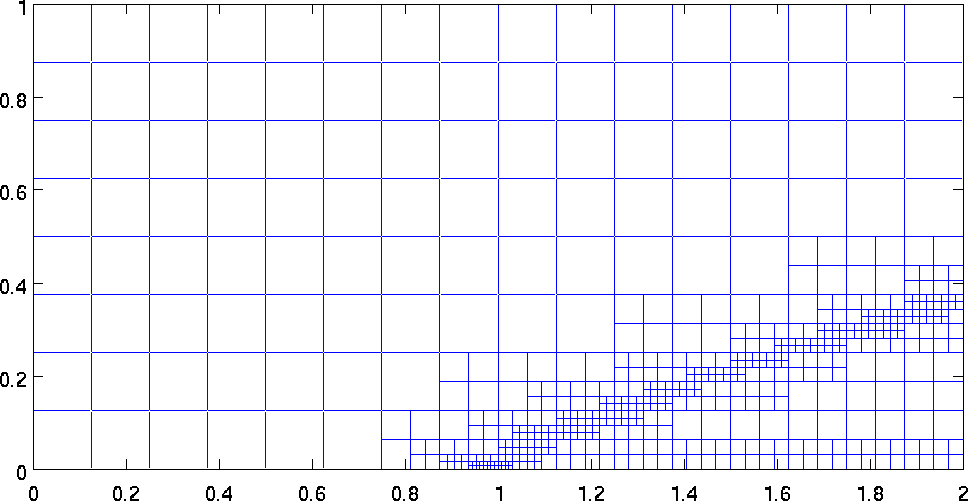
\includegraphics[scale = 0.45]{figures/mesh4.png}
}
\subfigure[i=5]{
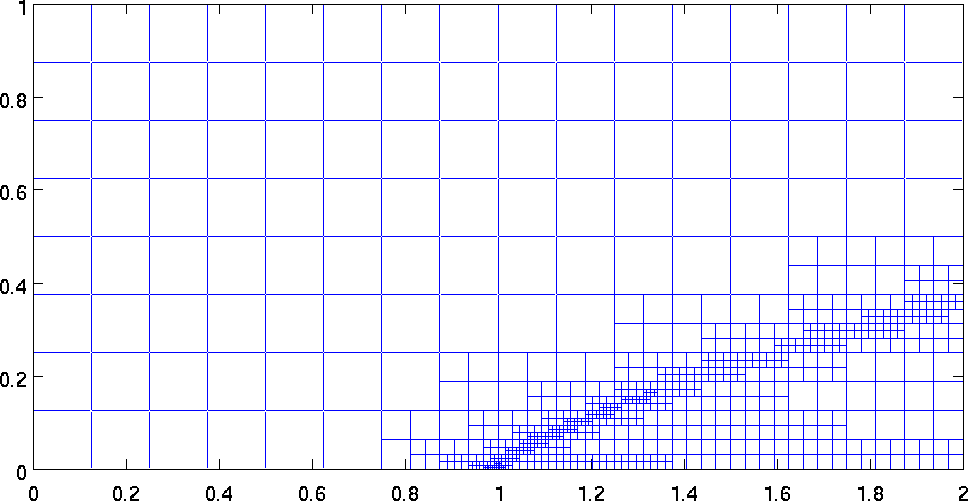
\includegraphics[scale = 0.45]{figures/mesh5.png}
}
\subfigure[i=6]{
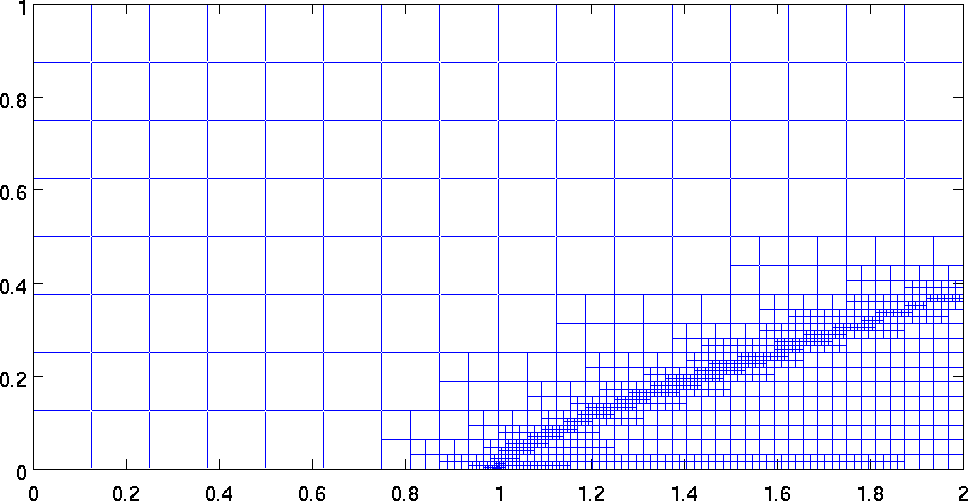
\includegraphics[scale = 0.45]{figures/mesh6.png}
}
\caption{Mesh refinements for compressible Navier-Stokes in Carter's flat plate problem.  The $i$ values are the refinement number (i.e. $i=0$ corresponds to the initial mesh).}
\label{fig:JCmeshRefinements}
\end{figure}

\begin{figure}[h!]
\centering
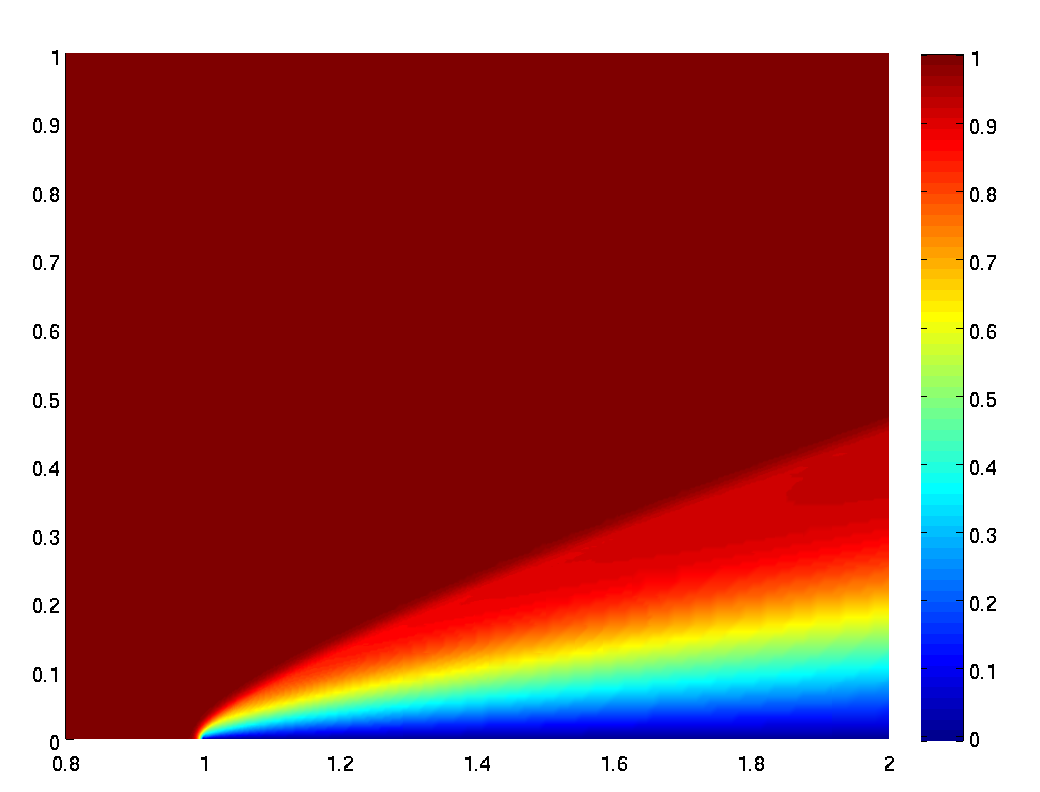
\includegraphics[scale = 0.90]{figures/u1.pdf}
\caption{Final solution for the $x$ component of the velocity in Carter's flat plate problem.}
\label{fig:JCu1}
\end{figure}

%\subsection{Meshing, Solving, and Adaptivity}\label{sec:Meshing}   both what's there now, and what we will eventually do.  This is where our idea for the $hp$-decision algorithm should go.
%\subsubsection{Handling Hanging Nodes: MultiBasis and PatchBasis}\label{sec:HangingNodes}
%\subsection{Nonlinear Problems}\label{sec:NonlinearProblems}
%\subsection{Comparison between Camellia and deal.II}\label{sec:Deal.II}
%\subsection{Summary}\label{sec:CamelliaConclusion}

\clearpage

\pagebreak
\section{Numerical Experiments for the Stokes Equations}
\label{sec:StokesNumericalResults}
To illustrate the theoretical results, we perform three numerical
experiments.  In the first two we use boundary conditions and forcing
function corresponding to a manufactured solution; first showing
optimal convergence using the graph norm arising from the analysis as
the test space norm, then showing sub-optimal convergence when a naive
norm is selected instead.  Finally, we examine the classic lid-driven
cavity flow problem.

We implemented the experiments described below using \emph{Camellia}, a toolbox for DPG developed by Roberts starting at Sandia in summer 2011, in collaboration with Denis Ridzal and Pavel Bochev \cite{RobertsEtAl11}.  Camellia supports 2D meshes of triangles and quads of variable polynomial order, provides mechanisms for easy specification of DPG variational forms, supports $h$- and $p$- refinements, and supports distributed computation of the stiffness matrix, among other features.

Recall that the pressure $p$ in the Stokes problem is only determined up to a constant.  Following a method described by Bochev and Lehoucq \cite{BochevLehoucq}, we add a constraint on the pressure that enforces
\[
\int_{\Omega} p = 0,
\]
thereby determining the solution uniquely.  This constraint is also satisfied by the manufactured solution used in our experiments.

Before turning to the experiments themselves, we briefly note the expected convergence properties and give a few implementation details.  When implementing DPG, we have several choices: what polynomial orders to use for the approximation of fields, traces, and fluxes; how to approximate the optimal test functions, and what norm to use on the test space.  We discuss each of these in turn.

\subsection{Convergence and orders of polynomial approximation}
For a DPG solution $(u_{h},\widehat{u}_{h})$ and exact solution $(u,\widehat{u})$, the analysis in Appendix \ref{sec:StokesAnalysis} gives us
\begin{align}\label{NVR:eqn:gammaBound}
\left(\norm{u-u_{h}}^{2} + \norm{\widehat{u}-\widehat{u}_{h}}_{\hat{H}_A(\Gamma_{h})}^{2}\right)^{1/2} \leq \frac{M}{\gamma_{DPG}} \inf_{(w_{h},\widehat{w}_{h})}\left(\norm{u-w_{h}}^{2} + \norm{\widehat{u}-\widehat{w}_{h}}_{\hat{H}_A(\Gamma_{h})}^{2}  \right)^{1/2},
\end{align}
where $M=O(1)$ and $\gamma_{DPG}=O(\gamma)$ (and for the Stokes problem, $\gamma=O(1)$), the salient point for convergence being that these are mesh-independent constants: for the graph norm presented in the analysis, the method is automatically stable.\footnote{As will be seen in what follows, if we use the naive test norm instead, we do \emph{not} get the optimal convergence rates in the pressure.  We hypothesize that if we performed a similar analysis for the naive norm, $\gamma$ would not be mesh-independent.}

Assuming $u$ is sufficiently smooth, for a discrete $L^2$ space comprised of polynomials of order $k$, we expect best $h$-convergence rates of $k+1$; that is, we have
\begin{align}
\inf_{w_{h} \in U_{h}} \norm{u-w_{h}} \leq C_{1} h^{k+1}.\label{NVR:eqn:hBound}
\end{align}
for some mesh-independent constant $C_{1}$.  It can be shown that, for traces $\widehat{w}_{h}$ whose $H^{-1/2}(\Gamma_{h})$ and $H^{1/2}(\Gamma_{h})$ components are approximated by polynomials of orders $k$ and $k+1$, respectively,
\[
\inf_{\widehat{w}_{h} \in \hat{H}_A(\Gamma_{h})} \norm{\widehat{u}-\widehat{w}_{h}}_{\hat{H}_A(\Gamma_{h})} \leq C_{2} h^{k+1}
\]
for some mesh-independent constant $C_{2}$.  For details and further references, see \cite[pp. 7-8]{DPG6}. Combining this with equations (\ref{NVR:eqn:gammaBound}) and (\ref{NVR:eqn:hBound}), we then have the bound
\[
\norm{u-u_{h}} \leq C h^{k+1}
\]
for $C = \min(C_{1}, C_{2})$.
Assuming negligible error in computing the optimal test functions, for these choices of polynomial order, we expect DPG solutions to converge in $h$ at the optimal rate of $k+1$ for all $L^{2}$ variables.

We can also motivate the choice of polynomial orders for the trial space intuitively from the exact sequence.  If we define $k$ as the polynomial order of approximation of field variables, because these belong to $L^{2}$, it is natural to choose $k+1$ as the $H^{1}$ order.  The traces of $H^{1}$ functions ($\widehat{u}_{1}$ and $\widehat{u}_{2}$) belong to $H^{1/2}$, a stronger space than $L^{2}$, so that $k+1$ is a natural order of approximation for these.  The traces of \NVRHdiv  functions $\left(\widehat{{\sigma_{11} - p \choose \sigma_{12}} \cdot \vect{n}}\right.$ and $\left.\widehat{{\sigma_{21}  \choose \sigma_{22} - p} \cdot \vect{n}}\right)$ belong to $H^{-1/2}$, a weaker space than $L^{2}$, so that $k$ is a natural order of approximation for these.

The exact optimal test functions will not in general be polynomials; we approximate them by using an ``enriched'' space of Lagrange and Raviart-Thomas elements approximating $H^{1}(\Omega_{h})$ and $\vect{H}(\text{\rm div},\Omega_{h})$ components of the test space.  In practice, we experiment with various levels of enrichment, and take the minimum enrichment that yields results nearly as good as higher levels of enrichment.  In the present work, we used 1 as the enrichment order; that is, $k_{\rm test} = k+2$.  As will be seen below, with this, we come extremely close to matching the best approximation error, so that there is no benefit to enriching the test space further.\footnote{For an analysis of the effect of the test space enrichment on rates of convergence in the Laplace problem and linear elasticity, see Gopalakrishnan and Qiu \cite{GopalakrishnanQiu11}.}

Note also that we have made no assumptions about the choice of basis functions.  The present work uses $H^{1}$- and \NVRHdiv-conforming nodal bases provided by the Intrepid package in Trilinos \cite{Trilinos}.

\subsection{Test space norm}
The choice of test norm arising from the above analysis is the (adjoint) graph norm:
\begin{align*}
\norm{(\NVRtensor{\tau},\vect{v}, q)}_{\rm graph}^{2} = \norm{\NVRdiv \NVRtensor{\tau} - \NVRgrad q}^{2} + \norm{\NVRdiv \vect{v}}^{2} + \norm{ \NVRtensor{\tau} + \NVRgrad{\vect{v}}}^{2} + \norm{\NVRtensor{\tau}}^{2} + \norm{\vect{v}}^{2} + \norm{q}^{2}
\end{align*}

We use this norm in our first experiment, and get the optimal convergence rates for the field variables.  In our second experiment, we consider another choice of test norm, which we refer to as the \emph{naive} test space norm:
\begin{align*}
\norm{(\NVRtensor{\tau},\vect{v}, q)}_{\rm naive}^{2} = \norm{\NVRtensor{\tau}}^{2} + \norm{\NVRdiv \NVRtensor{\tau}}^{2} + \norm{\vect{v}}^{2} + \norm{\NVRgrad \vect{v}}^{2} + \norm{q}^{2} + \norm{\NVRgrad q}^{2}.
\end{align*}
Note that this is a \emph{stronger} space than the one generated by the graph norm; that is, if we define
\begin{align*}
\V_{\rm graph} &= \{ (\NVRtensor{\tau},\vect{v}, q) : \norm{(\NVRtensor{\tau},\vect{v}, q)}_{\rm graph} < \infty \}, \text{and} \\
\V_{\rm naive} &= \{ (\NVRtensor{\tau},\vect{v}, q) : \norm{(\NVRtensor{\tau},\vect{v}, q)}_{\rm naive} < \infty \},
\end{align*}
then $V_{\rm naive} \subset V_{\rm graph}$.  Specifically, $V_{\rm graph}$ only requires $\NVRdiv \NVRtensor{\tau} - \NVRgrad q \in \vect{L}^{2}$, while $V_{\rm naive}$ requires $\NVRdiv \NVRtensor{\tau} \in \vect{L}^{2}$ \emph{and} $\NVRgrad q \in \vect{L}^{2}$.

\subsection{Manufactured Solution Experiment with Graph Test Space Norm}
To test the method, we use a manufactured solution following Cockburn et al. \cite{CockburnKanschatSchotzauSchwab03}
\begin{align*}
u_{1} &=  -e^{x} ( y \cos y + \sin y )\\
u_{2} &=  e^{x}  y \sin y\\
p &= 2 \mu e^{x} \sin y
\end{align*}
on domain $\Omega = (-1,1)^2$, taking $\mu=1$, with uniform quadrilateral meshes of increasing granularity, and examine convergence rates.  The $L^{2}$ norm of the exact solution for $u_{1}$ is 2.53; for $u_{2}$, 1.07; for $p$, 2.81.

Figures \ref{fig:graph_h} and \ref{fig:graph_p} show $h$- and $p$-convergence\footnote{In this context, by $p$ we mean polynomial refinements.  We mostly use $k$ for polynomial order, because $p$ is our pressure variable; but a few times in the following pages we will overload $p$ to mean polynomial order as well.} results using the graph norm in the test space, for uniform quadrilateral meshes varying from $k=1$ to 4 in polynomial order, and from $1 \times 1$ to $16 \times 16$ elements.  The dashed lines in the plots show the error of an $L^{2}$ projection of the exact solution (the theoretical best we could achieve)---the lines lie nearly on top of each other.  We not only observe optimal convergence rates, but almost exactly achieve the best approximation error!

\begin{figure}[h!b!p!]
\centering
\subfigure[$u_{1}$]{
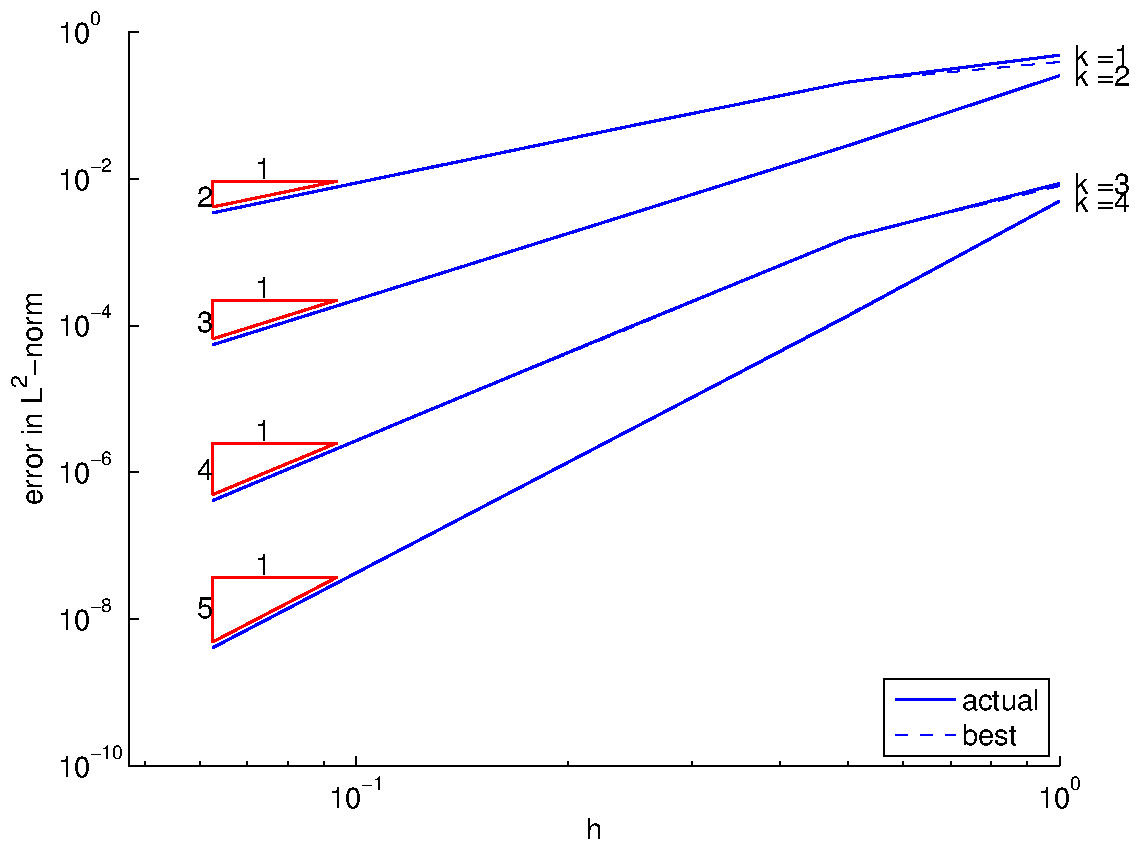
\includegraphics[scale=0.42]{./figures/u1_graph_h.pdf}
\label{fig:u1graph_h}
}
\subfigure[$u_{2}$]{
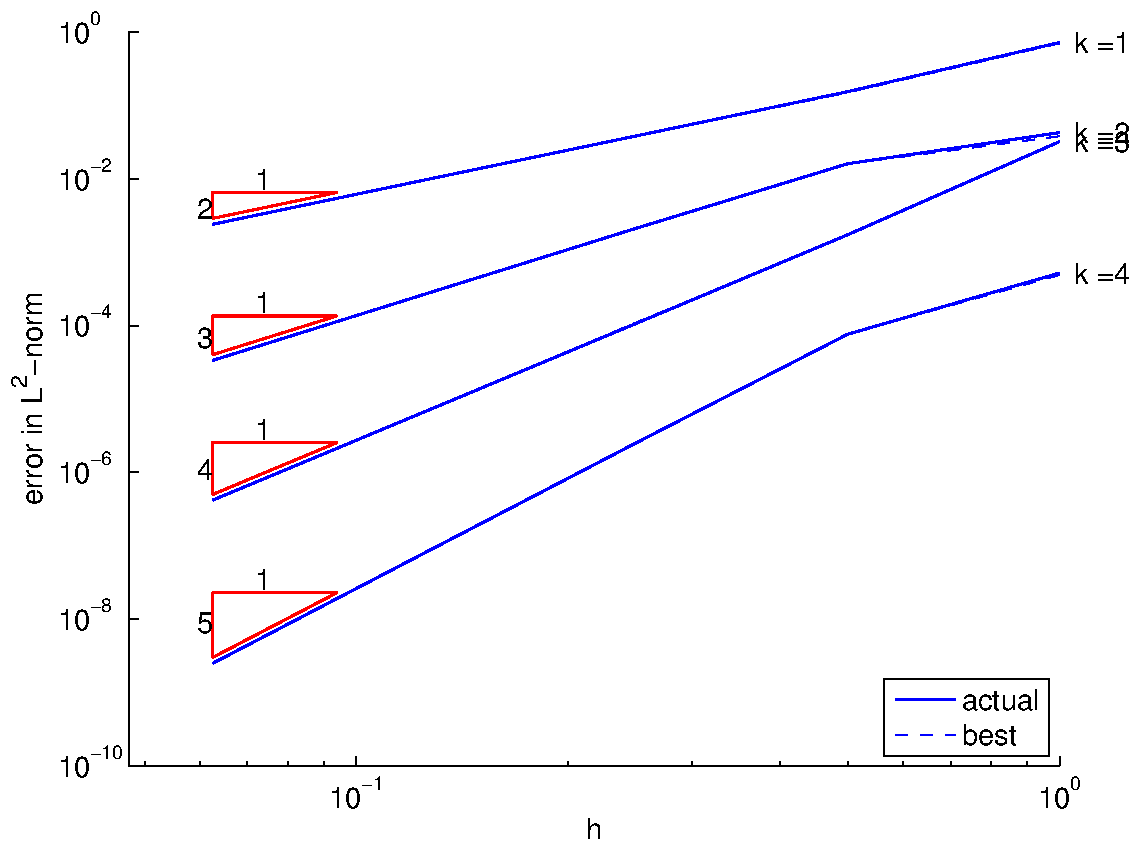
\includegraphics[scale=0.42]{./figures/u2_graph_h.pdf}
\label{fig:u2graph_h}
}
\subfigure[$p$]{
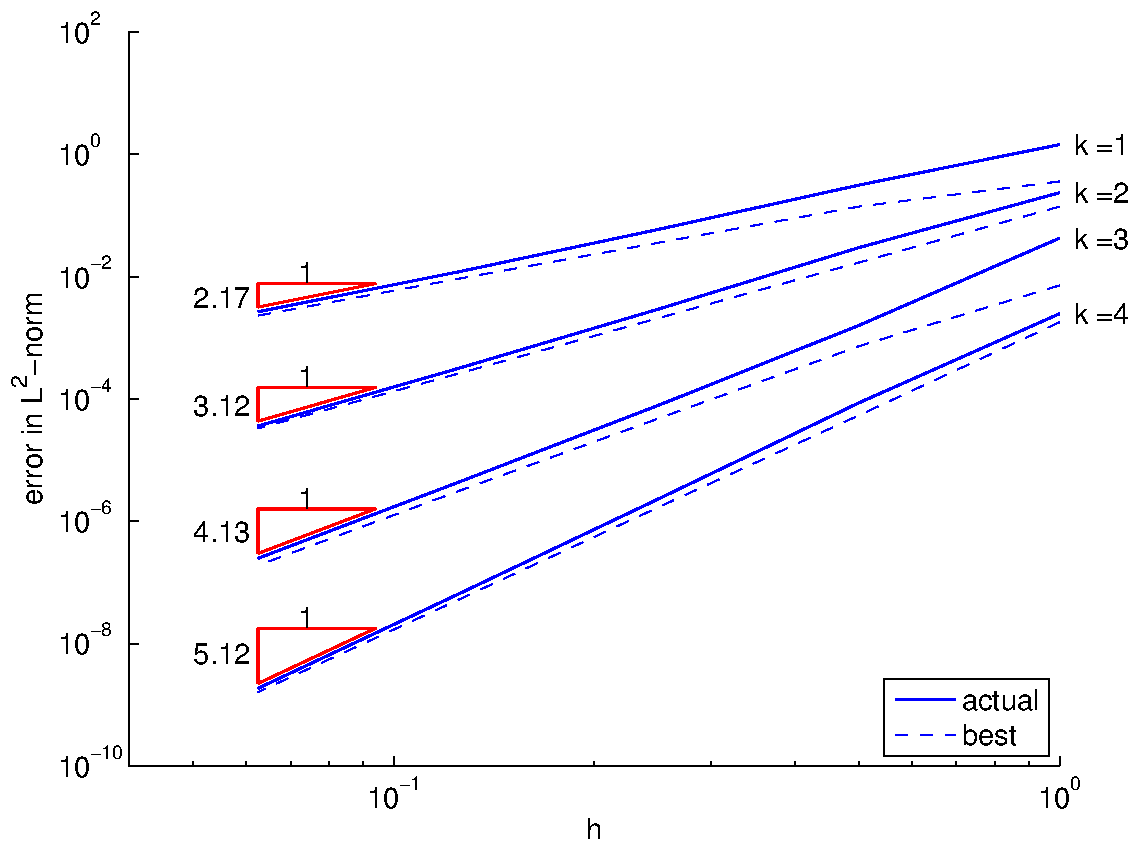
\includegraphics[scale=0.42]{./figures/pressure_graph_h.pdf}
\label{fig:pressuregraph_h}
}
\caption{$h$-convergence of $u_{1},u_{2}$ and $p$ when using the graph norm for the test space.  We observe optimal convergence rates, and nearly match the $L^{2}$-projection of the exact solution.
}
\label{fig:graph_h}
\end{figure}

\begin{figure}[h!b!p!]
\centering
\subfigure[$u_{1}$]{
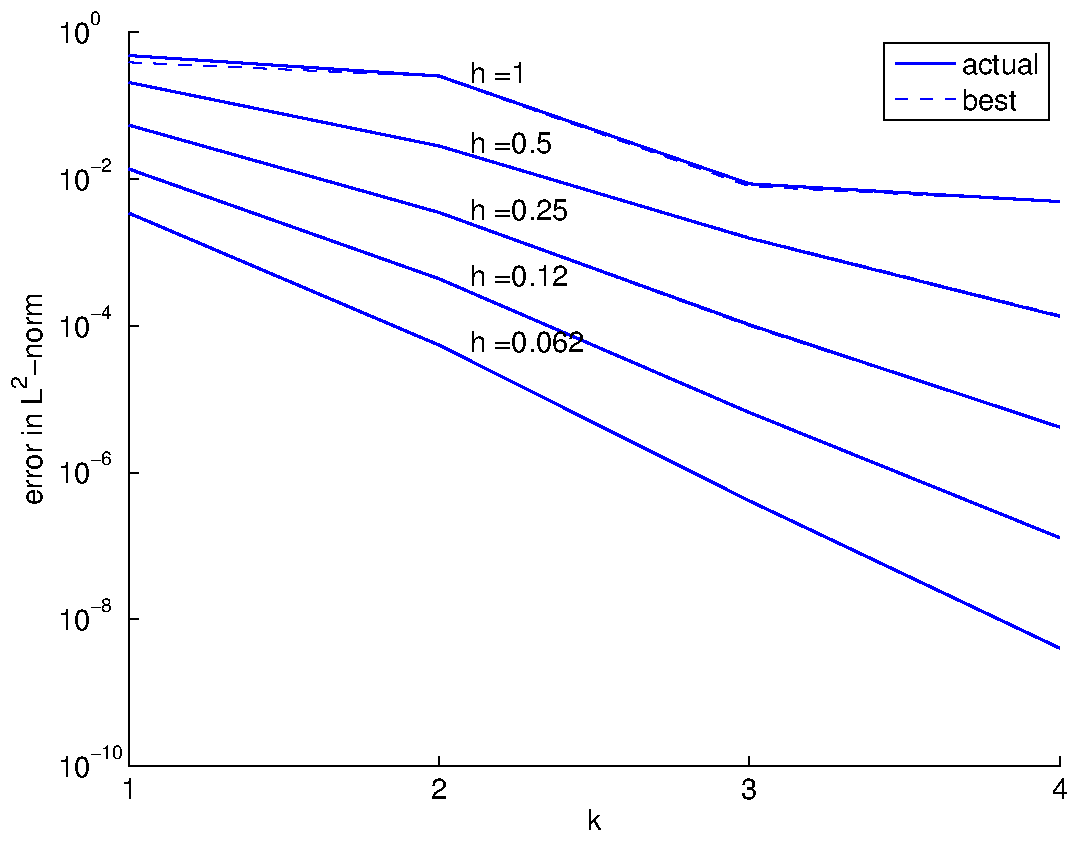
\includegraphics[scale=0.42]{./figures/u1_graph_p.pdf}
\label{fig:u1graph_p}
}
\subfigure[$u_{2}$]{
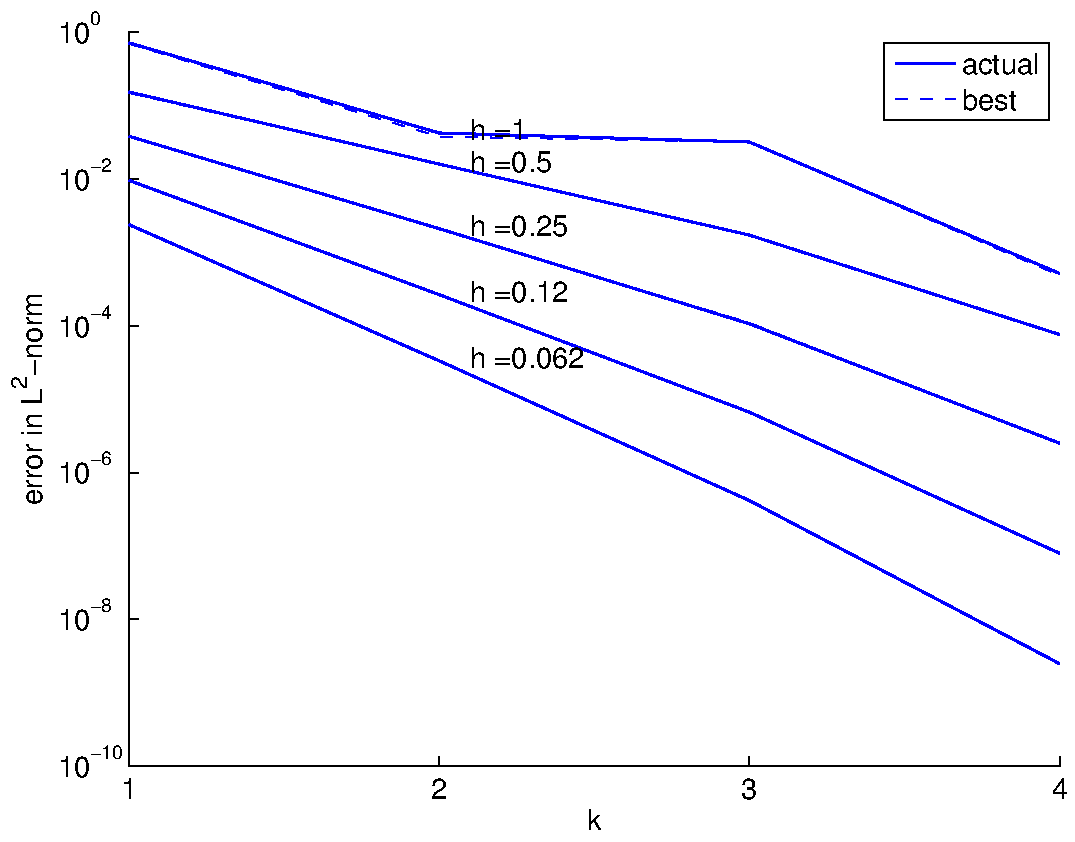
\includegraphics[scale=0.42]{./figures/u2_graph_p.pdf}
\label{fig:u2graph_p}
}
\subfigure[$p$]{
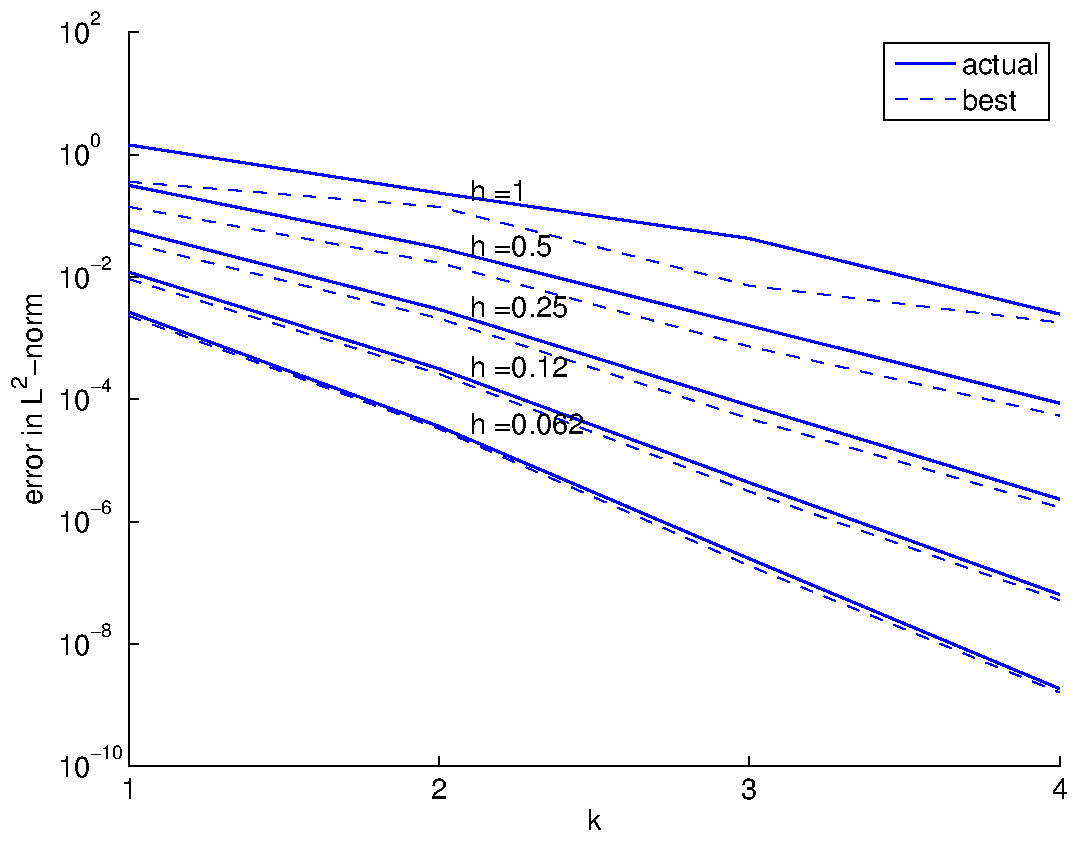
\includegraphics[scale=0.42]{./figures/pressure_graph_p.pdf}
\label{fig:pressuregraph_p}
}
\caption{p-convergence of $u_{1},u_{2}$ and $p$ when using the graph norm for the test space.  We observe exponential convergence for the finer meshes, and nearly match the $L^{2}$-projection of the exact solution.
}
\label{fig:graph_p}
\end{figure}

\subsection{Manufactured Solution Experiment with Naive Test Space Norm}
Our second manufactured solution experiment uses the naive norm on the test space.  This was the first norm we used when studying DPG formulations of Stokes \cite{RobertsetAl10}, before we had developed the analysis above, showing why the naive norm might not do as well as the graph norm does.

Figures \ref{fig:naive_h} and \ref{fig:naive_p} show $h$- and $p$-convergence results using the naive norm in the test space, for uniform quadrilateral meshes varying from $k=1$ to 4 in polynomial order, and from $1 \times 1$ to $16 \times 16$ elements; we have again plotted for comparison the error in the $L^{2}$ projection of the exact solution.  As with the graph norm, here we observe optimal convergence rates and almost exactly achieve the best approximation error in velocities $u_{1}$ and $u_{2}$, but in the pressure $p$ we are sub-optimal by up to two orders of magnitude.  

Why do we not see optimal convergence for the naive norm?  Recall that this is a stronger norm than the graph norm used in our analysis; thus the test functions that we seek---namely, the ones that will minimize the residual---may not reside within the continuous space represented by the naive norm.  By using the naive norm, we are searching for these test functions inside a smaller space, and we may not find them there.

\begin{figure}[h!b!p!]
\centering
\subfigure[$u_{1}$]{
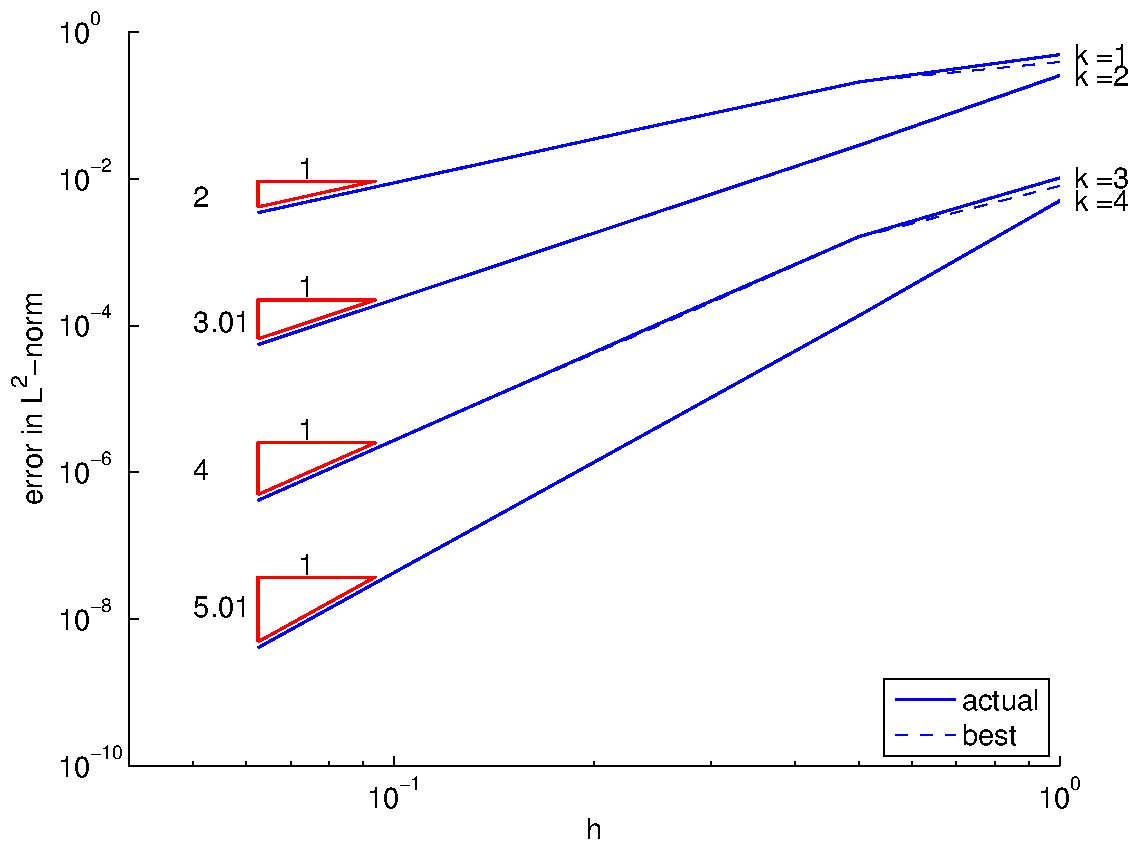
\includegraphics[scale=0.42]{./figures/u1_naive_h.pdf}
\label{fig:u1naive_h}
}
\subfigure[$u_{2}$]{
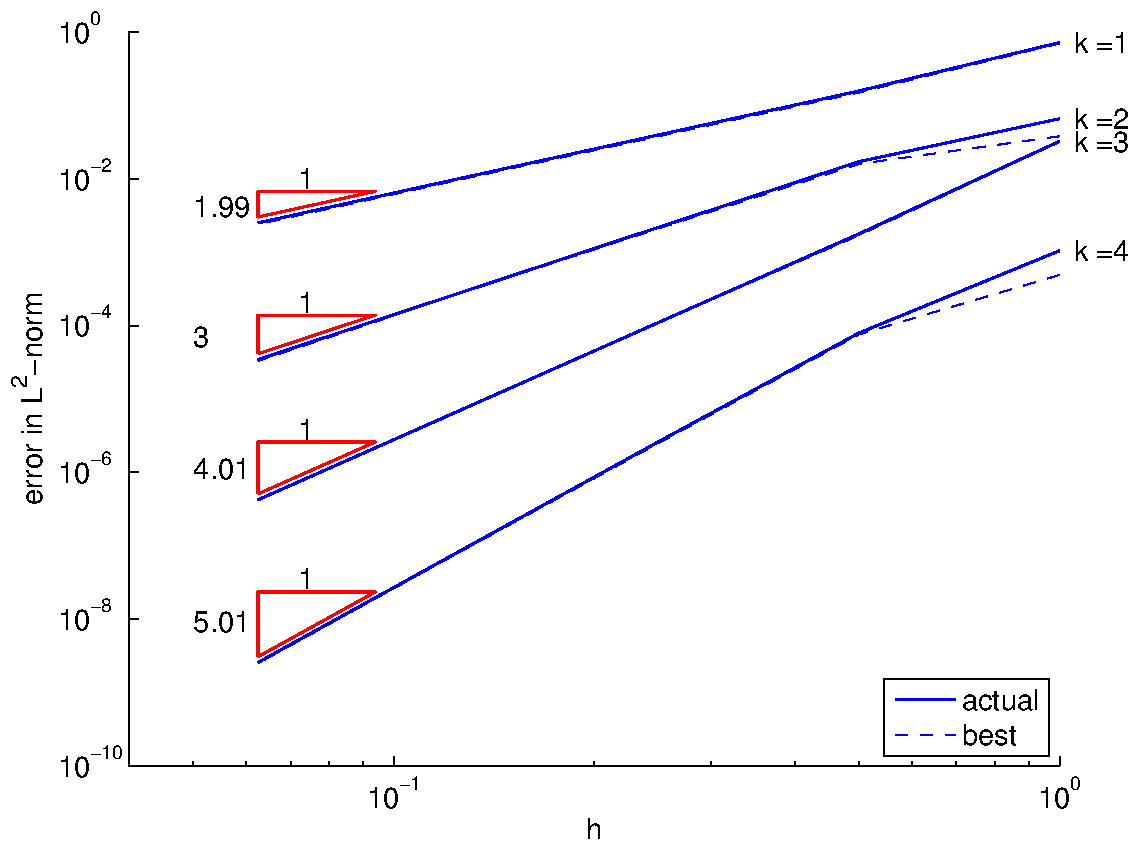
\includegraphics[scale=0.42]{./figures/u2_naive_h.pdf}
\label{fig:u2naive_h}
}
\subfigure[$p$]{
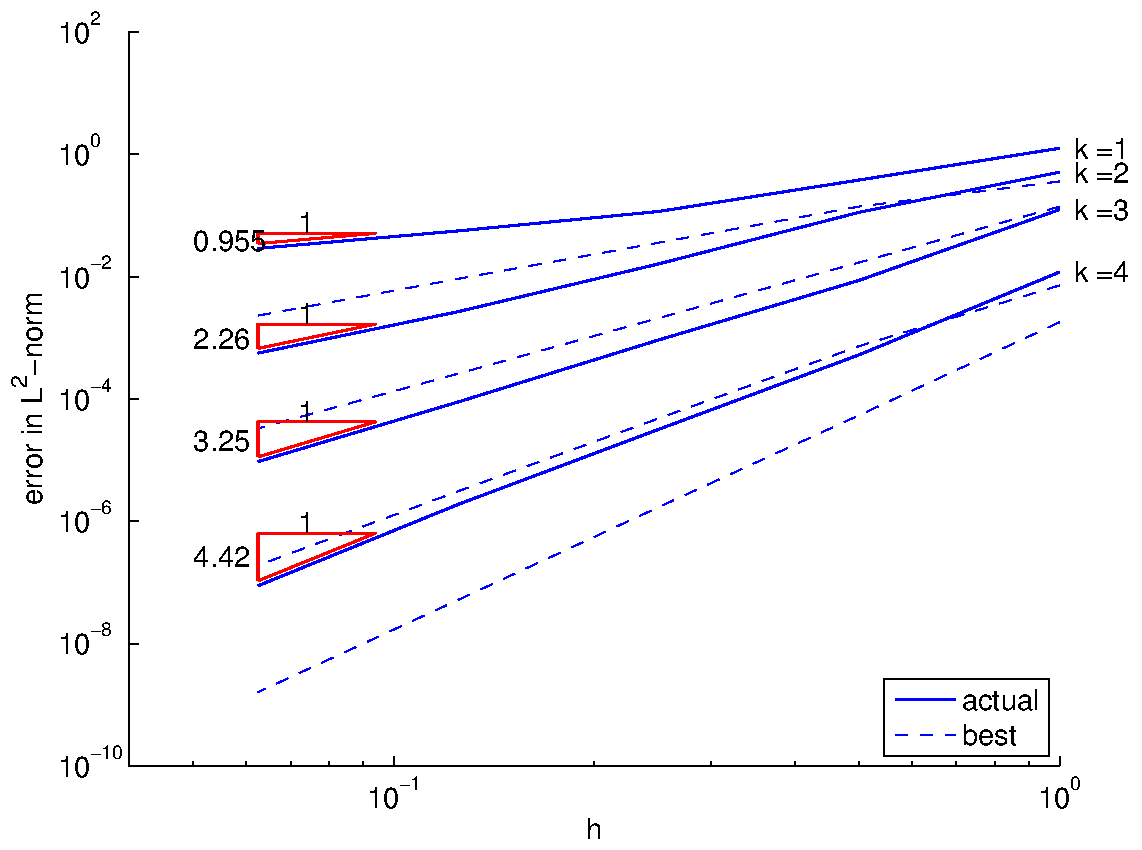
\includegraphics[scale=0.42]{./figures/pressure_naive_h.pdf}
\label{fig:pressurenaive_h}
}
\caption{$h$-convergence of $u_{1},u_{2}$ and $p$ when using the naive norm for the test space.  We observe optimal convergence rates (and nearly match the $L^{2}$-projection of the exact solution) for $u_{1}$ and $u_{2}$, but $p$ converges at suboptimal rates.
}
\label{fig:naive_h}
\end{figure}


\begin{figure}[h!b!p!]
\centering
\subfigure[$u_{1}$]{
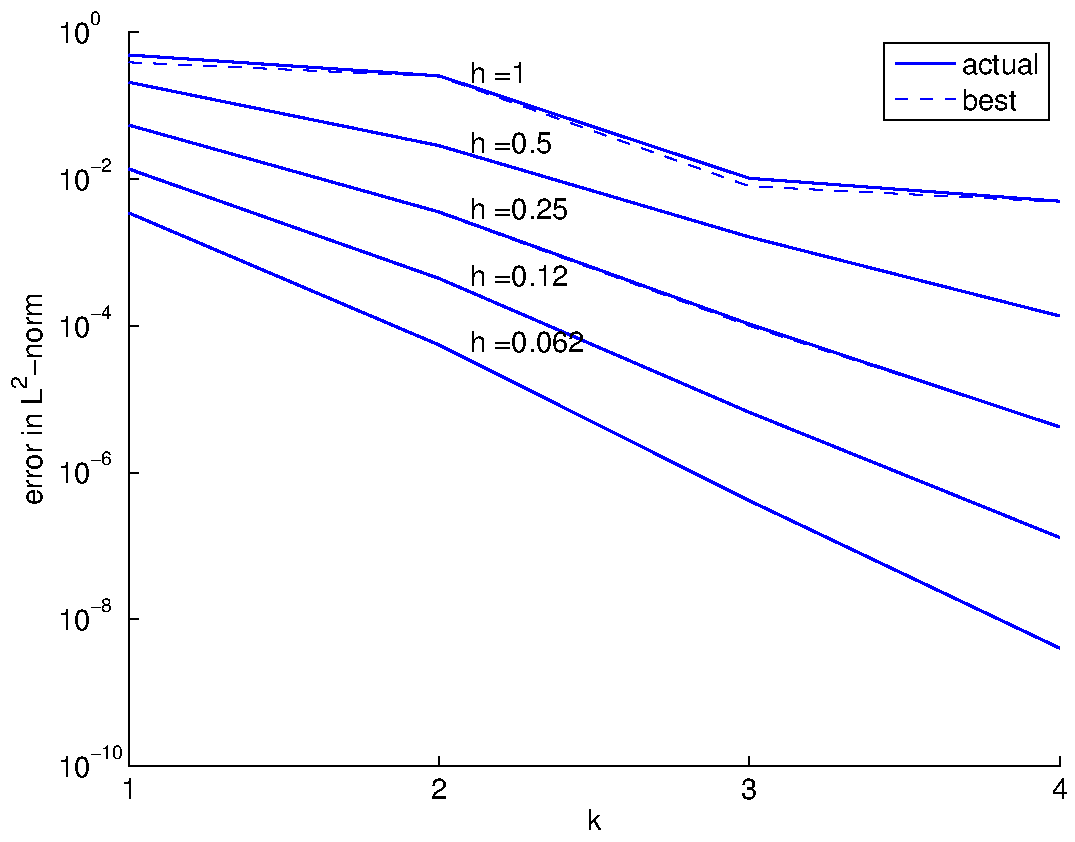
\includegraphics[scale=0.42]{./figures/u1_naive_p.pdf}
\label{fig:u1naive_p}
}
\subfigure[$u_{2}$]{
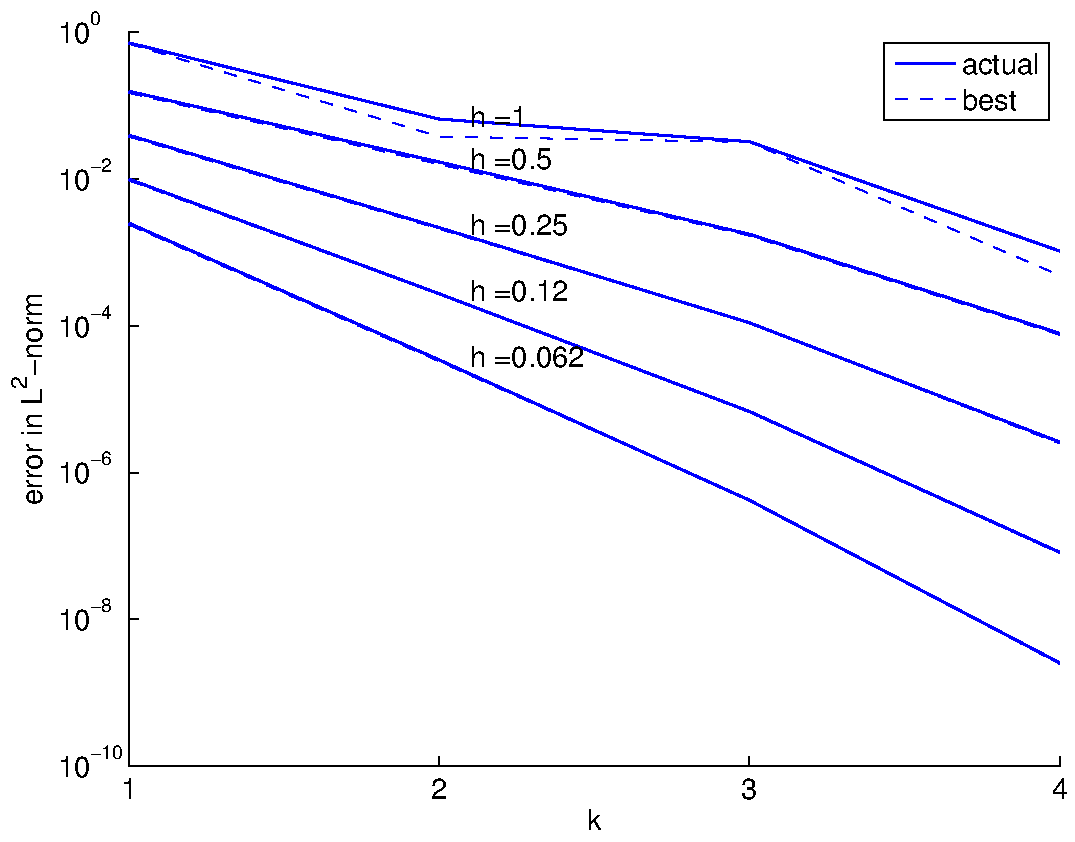
\includegraphics[scale=0.42]{./figures/u2_naive_p.pdf}
\label{fig:u2naive_p}
}
\subfigure[$p$]{
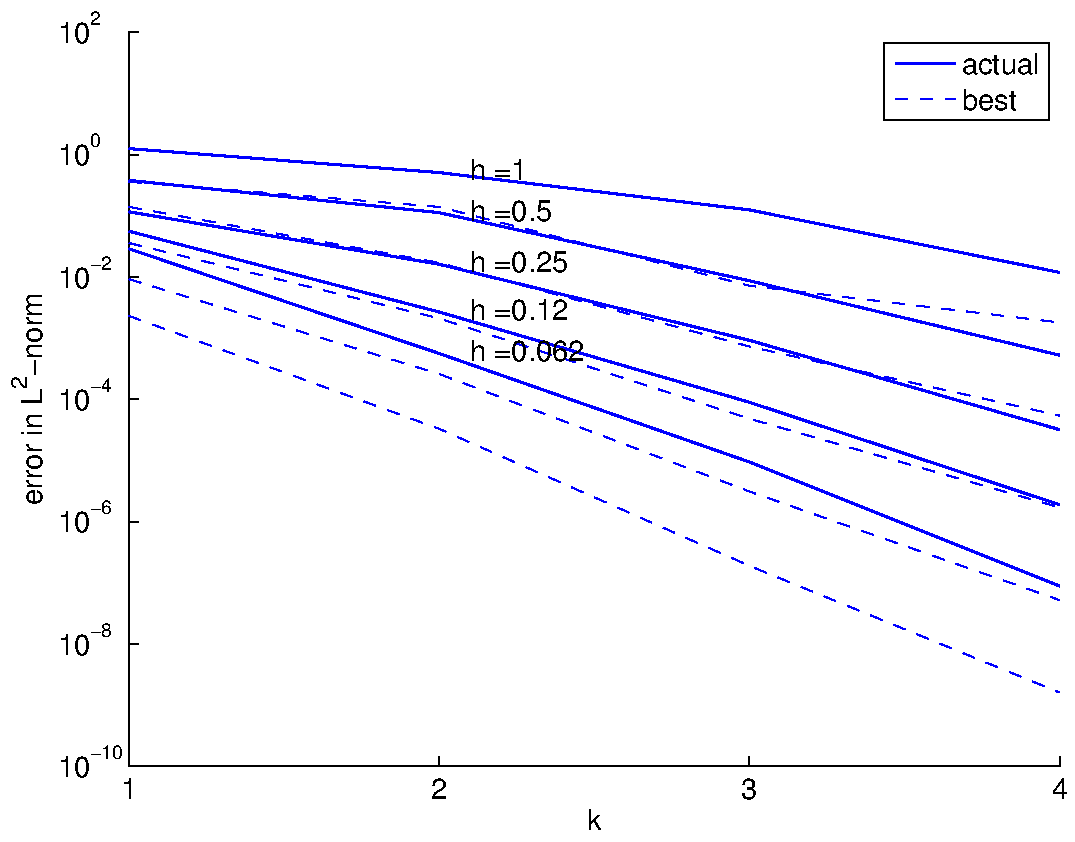
\includegraphics[scale=0.42]{./figures/pressure_naive_p.pdf}
\label{fig:pressurenaive_p}
}
\caption{p-convergence of $u_{1},u_{2}$ and $p$ when using the naive norm for the test space.  We observe exponential convergence for the finer meshes, and nearly match the $L^{2}$-projection of the exact solution for $u_{1}$ and $u_{2}$, but see significantly suboptimal solutions in $p$.
}
\label{fig:naive_p}
\end{figure}

\subsection{Lid-Driven Cavity Flow}
A classic test case for Stokes flow is the lid-driven cavity flow problem.  Consider a square cavity with an incompressible, viscous fluid, with a lid that moves at a constant rate.  The resulting flow will be vorticular; as sketched in Figure \ref{fig:cavity_flow_cartoon}, there will also be so-called \emph{Moffat eddies} at the corners; in fact, the exact solution  will have an infinite number of such eddies, visible at progressively finer scales \cite{Moffat}.  Note that the problem as described will have a discontinuity in the fluid velocity at the top corners, and hence its solution will not conform to the spaces we used in our analysis; for this reason, in our experiment we approximate the problem by introducing a thin ramp in the boundary conditions---we have chosen a ramp of width $\frac{1}{64}$.  This makes the boundary conditions continuous,\footnote{It is worth noting that these boundary conditions are not exactly representable by many of the coarser meshes used in our experiments.  We interpolate the boundary conditions in the discrete space.} so that the solution conforms to the spaces used in the analysis.
\begin{figure}[h!b!p!]
\centering
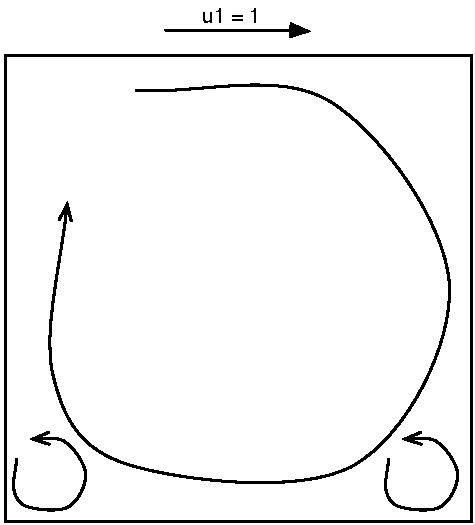
\includegraphics[scale=0.42]{./figures/cavity_flow_cartoon.pdf}
\caption{Sketch of lid-driven cavity flow.
}
\label{fig:cavity_flow_cartoon}
\end{figure}

As described in the introduction, DPG gives us a mechanism for measuring the residual error in the dual norm (the very error we seek to minimize) precisely, and we use this to drive adaptivity, by measuring the error $\norm{e_{K}}_{V}$ for each element $K$.  Both the method and our code allow refinements in $h$ or $p$ or in some combination of $h$ and $p$.  However, we do not yet have a general mechanism for deciding \emph{which} refinement to apply ($h$ or $p$), once we have decided that a given element should be refined.  We run two experiments, one with $h$-adaptivity and one using an ad hoc $hp$-adaptive strategy, described below.

Although it is not required by the code, we enforce \emph{1-irregularity} throughout---that is, before an element can be refined twice along an edge, its neighbor along that edge must be refined once.  In limited comparisons running the same experiments without enforcing 1-irregularity, this did not appear to make much practical difference.

\subsubsection{$h$-refinement strategy}
For $h$-refinements, our strategy is very simple:
\begin{enumerate}
\item Loop through the elements, determining the maximum element error $\norm{e_{K{\rm max}}}_{V}$.
\item Refine all elements with error at least 20\% of the maximum $\norm{e_{K{\rm max}}}_{V}$.
\end{enumerate}

Because the exact solution is unknown, we first solve on an overkill mesh and compare our adaptive solution at each step to the overkill solution.  In this experiment, we used quadratic field variables ($k=2$), a test space enrichment of 1 relative to the $H^{1}$ order (that is, $k_{\rm test} = k + 2 = 4$) for both the adaptive and overkill solutions.  The overkill mesh was $256 \times 256$ elements, with 5,576,706 dofs.

The initial mesh was a $2 \times 2$ square mesh; we ran seven $h$-adaptive refinements.  We stopped after seven steps to ensure that the resulting mesh was nowhere finer than the overkill solution.  At each step, we computed the Euclidean ($\ell_{2}$) norm of the $L^{2}$ norm of each of the seven field variables.  The final adaptive mesh has 124 elements and 11,202 dofs, and combined $L^{2}$ error of $4.4 \times 10^{-4}$ compared with the overkill mesh.  We also ran a few uniform refinements and computed the $L^{2}$ error for these compared with the overkill mesh, to show the comparative efficiency of the adaptive refinements.  The results are plotted in Figure \ref{fig:adaptive_cavity_flow_quadratic_vs_overkill}.
\begin{figure}[h!b!p!]
\centering
\includegraphics[scale=0.60]{./figures/adaptive_cavity_flow_quadratic_vs_overkill.pdf}
\caption{Euclidean norm of $L^{2}$ error in all field variables in $h$-adaptive mesh relative to an overkill mesh with $256 \times 256$ quadratic elements.  The Euclidean norm of all field variables in the exact solution is 6.73.
}
\label{fig:adaptive_cavity_flow_quadratic_vs_overkill}
\end{figure}

We also post-processed the results to solve for the stream function $\phi$, where $\Delta \phi = \NVRcurl \vect{u}$.  The contours of $\phi$ are the streamlines of the flow.  These are plotted for the quadratic adaptive mesh described above in Figure \ref{fig:streamlines_p2}; the first Moffat eddy can be seen clearly in the zoomed-in plot.  This quadratic mesh does not resolve the second Moffat eddy, but if we run 11 adaptive refinements on a cubic mesh, we can see it.  This is shown in Figure \ref{fig:streamlines_p3_r11}.

\begin{figure}[h!b!p!]
\centering
\subfigure[full cavity]{
\includegraphics[scale=0.42]{./figures/streamlines_p2_r7.pdf}
\label{fig:streamlines_p2_r7}
}
\subfigure[lower-left corner]{
\includegraphics[scale=0.42]{./figures/streamlines_detail_p2_r7.pdf}
\label{fig:streamlines_detail_p2_r7}
}
\caption{Streamlines for the full cavity and for the lower-left corner, on a quadratic mesh after 7 adaptive refinements.  The lower-left corner shows the first Moffat eddy.  The final mesh has 124 elements and 11,202 dofs.}
\label{fig:streamlines_p2}
\end{figure}

\begin{figure}[h!b!p!]
\centering
\includegraphics[scale=0.42]{./figures/streamlines_minute_detail_p3_r11.pdf}
\caption{Streamlines for the lower-left corner on a cubic mesh after 11 adaptive refinements: the second Moffat eddy.  The final mesh has 298 elements and 44,206 dofs.}
\label{fig:streamlines_p3_r11}
\end{figure}

\subsubsection{Ad hoc $hp$-refinement strategy}
For the $hp$ experiment, we adopt a similar strategy; this time, our overkill mesh contains $64 \times 64$ quintic elements, and our initial mesh has $2 \times 2$ linear elements.  We know {\it a priori} that we should refine in $h$ at the top corners---if only to fully resolve the boundary condition.  The strategy is again:
\begin{enumerate}
\item Loop through the elements, determining the maximum element error $\norm{e_{K{\rm max}}}_{V}$.
\item Refine all elements with error at least 20\% of the maximum $\norm{e_{K{\rm max}}}_{V}$.
\end{enumerate}
However, this time we must decide whether to refine in $h$ or $p$.  The basic constraints we would like to follow are:
\begin{itemize}
\item the adaptive mesh must be nowhere finer than the overkill mesh (in $h$ or $p$), and
\item prefer $h$-refinements at all corners (top and bottom).
\end{itemize}
So, once the corner elements are as small as the overkill mesh, then they refine in $p$, and all other elements refine in $p$ until they are quintic, after which they may refine in $h$.

The primary purpose of this experiment is to demonstrate that the method allows arbitrary meshes of arbitrary, variable polynomial order.  The strategy described above clearly depends on \emph{a priori} knowledge of the particular problem we are solving; we have yet to determine a good general strategy for deciding between $h$- and $p$-refinements.

We ran 9 refinement steps.  The final mesh has 46 elements and 5,986 dofs, compared with 1,223,682 dofs in the overkill mesh.  The $L^{2}$ error of the adaptive solution compared with the overkill is $8.0 \times 10^{-4}$.  As in the previous experiment, we also tried running a few uniform $h$-refinements on the same initial mesh, as a baseline for comparison.  The results are plotted in Figure \ref{fig:hp_adaptive_cavity_flow_vs_overkill}; the mesh can be seen in Figure \ref{fig:cavityFlowPolyOrder}.

\begin{figure}[h!b!p!]
\centering
\includegraphics[scale=0.60]{./figures/hp_adaptive_cavity_flow_vs_overkill.pdf}
\caption{Euclidean norm of $L^{2}$ error in all field variables in (ad hoc) $hp$-adaptive mesh relative to an overkill mesh with $64 \times 64$ quintic elements.  The Euclidean norm of all field variables in the exact solution is 6.73; the final mesh has 46 elements and 5,986 dofs.
}
\label{fig:hp_adaptive_cavity_flow_vs_overkill}
\end{figure}

\begin{figure}[h!b!p!]
\centering
\includegraphics[scale=0.60]{./figures/cavityFlowPolyOrder.pdf}
\caption{Adaptive mesh for ad hoc $hp$-adaptivity strategy after 9 refinement steps.  The scale represents the polynomial order of the $L^{2}$ variables in the solution.  The final mesh has 46 elements and 5,986 dofs.
}
\label{fig:cavityFlowPolyOrder}
\end{figure}

%\section{Overview of Incompressible Flow}
%Discussion of the full transient, nonlinear problem, plus simplified versions:
%\begin{itemize}
%\item full transient
%\item steady
%\item Oseen
%\item Stokes
%\end{itemize}

\bibliography{./DPG}
\bibliographystyle{plain}

%\pagebreak
%
%\section*{Appendix}
%\input{stokes_bounded_below}

%\input{detailedTables}




\end{document}
